\documentclass[11pt,a4paper]{report}
\newcommand{\volumetitle}{Reference}
% Shared preamble of the two volumes of the manual: user_manual.tex (Volume 1, User Manual) and reference.tex
% (Volume 2, Reference and Verification). Each volume loads the class (report, 11pt, a4paper) and
% defines \volumetitle before reading this file.
\usepackage[T1]{fontenc}
\usepackage{mathpazo}
\usepackage[scaled=0.92]{helvet}
\usepackage[varqu,varl,scaled=0.96]{zi4}   % Inconsolata: a narrower, clearer monospace than Courier
\usepackage[protrusion=true,expansion=true]{microtype}
\DisableLigatures[-]{encoding=T1,family=tt*}   % "--" in \cmd{} stays two hyphens (not an en dash)
\usepackage[a4paper,margin=2.5cm,headheight=14pt]{geometry}
\usepackage{amsmath,amssymb}
\usepackage{booktabs,longtable,array,tabularx,multirow}
\usepackage{graphicx}
\usepackage[table]{xcolor}
\definecolor{brand}{HTML}{1F4E79}
\definecolor{brandlight}{HTML}{E3ECF6}
\definecolor{rowgray}{gray}{0.965}
\usepackage{tikz}
\usetikzlibrary{arrows.meta,positioning,shapes.geometric,calc,fit,backgrounds,decorations.pathmorphing,patterns}
\usepackage{algorithm}
\usepackage{algpseudocode}
\usepackage{listings}
\usepackage{caption}
\captionsetup{font=small,labelfont={bf,color=brand},skip=6pt}
\captionsetup[table]{position=top}
\usepackage[most]{tcolorbox}
\usepackage{needspace}
\usepackage{float}
\usepackage{etoolbox}
\usepackage{titlesec}
\titleformat{\chapter}[display]{\normalfont\color{brand}}{\sffamily\large\bfseries\MakeUppercase{\chaptertitlename}\ \thechapter}{4pt}{\raggedright\sffamily\huge\bfseries}[\vspace{3pt}{\titlerule[0.8pt]}]
\titlespacing*{\chapter}{0pt}{0pt}{18pt}
\titleformat{\section}{\needspace{8\baselineskip}\raggedright\normalfont\sffamily\Large\bfseries\color{brand}}{\thesection}{0.7em}{}
\titleformat{\subsection}{\needspace{6\baselineskip}\raggedright\normalfont\sffamily\large\bfseries\color{brand!80!black}}{\thesubsection}{0.7em}{}
\titleformat{\subsubsection}{\needspace{6\baselineskip}\normalfont\sffamily\normalsize\bfseries}{\thesubsubsection}{0.7em}{}
\titlespacing*{\section}{0pt}{16pt plus 4pt minus 2pt}{6pt}
\titlespacing*{\subsection}{0pt}{12pt plus 3pt minus 2pt}{4pt}
\usepackage{fancyhdr}
\pagestyle{fancy}
\fancyhf{}
\fancyhead[L]{\small\sffamily\color{gray}\leftmark}
\fancyhead[R]{\small\sffamily\color{gray}Raven--MODFLOW~6 coupling: \volumetitle}
\fancyfoot[C]{\small\sffamily\thepage}
\renewcommand{\headrulewidth}{0.4pt}
\renewcommand{\chaptermark}[1]{\markboth{\thechapter\quad #1}{}}
\fancypagestyle{plain}{\fancyhf{}\fancyfoot[C]{\small\sffamily\thepage}\renewcommand{\headrulewidth}{0pt}}
\usepackage{xr-hyper}   % references into the other volume (\externaldocument)
\usepackage[colorlinks=true,linkcolor=brand,citecolor=brand,urlcolor=brand]{hyperref}
\emergencystretch=6em
\setcounter{secnumdepth}{3}
\setcounter{tocdepth}{1}
\makeatletter\patchcmd{\l@chapter}{\addvspace{1.0em \@plus\p@}}{\addvspace{0.45em \@plus\p@}}{}{}\makeatother
\makeatletter\renewcommand*\l@section{\@dottedtocline{1}{1.5em}{2.9em}}\makeatother   % room for section numbers such as 10.11 and A.15
% ---- tables: small type, ragged-right columns, air between rows, shaded header row
\renewcommand{\arraystretch}{1.25}
\setlength{\tabcolsep}{5pt}
\AtBeginEnvironment{tabular}{\small}
\AtBeginEnvironment{tabularx}{\small}
\AtBeginEnvironment{longtable}{\small}
\newcolumntype{P}[1]{>{\raggedright\arraybackslash}p{#1}}
\newcolumntype{Y}{>{\raggedright\arraybackslash}X}
\newcommand{\hdr}{\rowcolor{brandlight}}
% ---- diagrams: the manual's sans-serif font; no hyphenation inside boxes
\tikzset{every picture/.prefix style={execute at begin picture={\sffamily}},
         every node/.append style={execute at begin node={\sffamily\hyphenpenalty=10000\exhyphenpenalty=10000}}}
% ---- code listings
\lstset{basicstyle=\ttfamily\footnotesize,columns=fullflexible,frame=single,framerule=0.3pt,rulecolor=\color{gray!50},breaklines=true,
        xleftmargin=4pt,xrightmargin=4pt,backgroundcolor=\color{gray!5},aboveskip=6pt,belowskip=6pt}
\newcommand{\ubreak}{\textunderscore}  % code names are not broken at underscores; a long one moves to the next line
\DeclareRobustCommand{\cmd}[1]{\begingroup\ttfamily\let\_\ubreak #1\endgroup}
\newcommand{\dt}{\Delta t}
% ---- boxes
\tcbset{boxrule=0.6pt,arc=2pt,left=5pt,right=5pt,top=3pt,bottom=3pt,fonttitle=\bfseries\small\sffamily}
\newtcolorbox{plain}{colback=teal!4,colframe=teal!55!black,title=In plain words}
\newtcolorbox{example}[1][]{colback=orange!4,colframe=orange!70!black,title=Worked example#1}
\newtcolorbox{watch}{colback=red!3,colframe=red!55!black,title=Watch out}
\newtcolorbox{inpractice}{colback=green!4,colframe=green!45!black,title=In practice}
\newtcolorbox{whattowrite}{colback=brandlight!40,colframe=brand,title=What to write}
\newtcolorbox{refcard}[1]{colback=brandlight!40,colframe=brand,title={Reference card: #1},breakable,enhanced jigsaw,before skip=10pt,after skip=10pt}

\externaldocument[U-]{user_manual}[Raven_MF6_User_Manual.pdf]   % Volume 1: \ref{U-label}
\begin{document}
\pagenumbering{Alph}
\begin{titlepage}
\centering
\vspace*{3.5cm}
{\color{brand}\rule{\linewidth}{1.2pt}}\par\vspace{16pt}
{\sffamily\bfseries\fontsize{30}{38}\selectfont\color{brand}Raven--MODFLOW~6\\[4pt]Groundwater Coupling\par}
\vspace{10pt}
{\sffamily\bfseries\LARGE\color{brand}Volume 2: Reference and Verification\par}
\vspace{14pt}
{\color{brand}\rule{\linewidth}{1.2pt}}\par\vspace{24pt}
{\large Manual chapter for the Raven Hydrological Modelling Framework\\[2pt](based on Raven 4.15)\par}
\vfill
{\sffamily\Large\bfseries Rezgar Arabzadeh\par}
\vspace{4pt}
{\large Principal Scientist, Hazen and Sawyer\par}
\vspace{2cm}
{\large November 2026\par}
\vspace{1.2cm}
{\footnotesize\color{gray!70!black}\copyright\ 2026 Rezgar Arabzadeh. This manual is licensed under the Creative Commons Attribution 4.0
International License (CC BY 4.0), \url{https://creativecommons.org/licenses/by/4.0/}.\par}
\end{titlepage}
\pagenumbering{roman}
\begingroup\small\tableofcontents\endgroup
\cleardoublepage
\chapter*{About this volume}\addcontentsline{toc}{chapter}{About this volume}\markboth{About this volume}{}
The manual of the Raven--MODFLOW~6 coupling has two volumes. Volume~1, the \emph{User Manual}
(\cmd{Raven\_MF6\_User\_Manual.pdf}), is written for modellers who are new to the coupling: what it does, which option to
use, what to write in the input files, and how to read the results. This volume, \emph{Reference and Verification}
(\cmd{Raven\_MF6\_Reference.pdf}), holds the detail behind it: every rule, equation and safeguard, the full command and
message tables, the tests, and the developer guide.

It is meant for looking things up. Each chapter starts with a short note on what it covers and where the User Manual
treats the same subject in plain terms. References of the form ``User Manual, Chapter~2'' point to Volume~1.
\begin{table}[!htbp]\centering
\caption{Where to find what in this volume.}\label{tab:refguide}
\begin{tabularx}{\linewidth}{P{0.34\linewidth}Y}\toprule\hdr
If you want to\dots & Read\\\midrule
recall the groundwater ideas behind the equations & Chapter~\ref{ch:c2}\\
know exactly how Raven builds the grid and the layers & Chapter~\ref{ch:c3}\\
know what happens to an existing MODFLOW~6 model & Chapter~\ref{ch:existing}\\
see the equations and safeguards of each exchange & Chapter~\ref{ch:c4}\\
follow the water accounts, the time step and restarts & Chapter~\ref{ch:c5}\\
look up a command or an output column & Chapter~\ref{ch:c6} and Appendix~\ref{app:tables}\\
find a message & Sections~\ref{app:errors} and~\ref{app:warnings}\\
see how the code was tested & Chapter~\ref{ch:c8}\\
change the code & Chapter~\ref{ch:c9}\\\bottomrule
\end{tabularx}
\end{table}
\cleardoublepage
\pagenumbering{arabic}
\chapter{Groundwater concepts}\label{ch:c2}\label{ch:concepts}
\noindent\emph{About this chapter.} The User Manual introduces these ideas in plain words (User Manual,
Section~\ref{U-sec:newraven}). This chapter gives the physics and the few equations that the later chapters build on.

This chapter introduces the physical ideas and vocabulary used in the rest of the document. Readers familiar with
groundwater hydrology can skim it; everyone else will find every later equation built from the few ideas presented here.


\section{Head}
The \emph{head} $h$ at a point is the elevation to which water would rise in a small well drilled to that point, in
metres above a common datum (here, the same datum as the digital elevation model). Groundwater always flows from
higher head to lower head. In an unconfined aquifer the head is the elevation of the water table; the \emph{depth to
water} is land-surface elevation minus head.

\section{Darcy's law}
The flow of water through a porous material is proportional to the drop in head and to the cross-section, and
inversely proportional to the distance travelled:
\begin{equation}
Q = K\,A\,\frac{h_1-h_2}{L},
\end{equation}
where $Q$ is the flow [m$^3$/d], $K$ the hydraulic conductivity [m/d], $A$ the area the water passes through [m$^2$],
$h_1-h_2$ the head difference [m] and $L$ the distance [m].

\begin{example}[: Darcy's law]
Gravel with $K=50$ m/d, a 2\,000 m wide and 10 m thick strip ($A=20\,000$ m$^2$), heads 101 m and 100 m, 2\,000 m apart:
$Q=50\times20\,000\times1/2\,000=500$ m$^3$/d.
\end{example}

\section{Transmissivity and conductance}
Because $K$, $A$ and $L$ always appear together, it is convenient to combine them into a \emph{conductance}
$C = K A/L$ [m$^2$/d], so that $Q=C\,(h_1-h_2)$. Every exchange in this document --- between two grid cells, between an
aquifer and a river, a drain, a wetland --- is written in this form: \textbf{flow = conductance $\times$ head
difference}. For a layer of saturated thickness $b$, the \emph{transmissivity} is $T=Kb$ [m$^2$/d].

Between two neighbouring cells with different conductivities $K_1,K_2$, the conductance is the series combination
(harmonic mean), because water must pass through both halves in turn:
\begin{equation}
C_{12}=\frac{1}{\dfrac{L_1}{K_1A}+\dfrac{L_2}{K_2A}} .
\end{equation}
\begin{example}[: harmonic mean]
Two 2\,000 m cells, 10 m thick and 2\,000 m wide ($A=20\,000$ m$^2$, $L_1=L_2=1\,000$ m to the shared face), gravel
$K_1=50$ m/d next to till $K_2=0.2$ m/d:
$C_{12}=1/(1\,000/(50\cdot20\,000)+1\,000/(0.2\cdot20\,000)) = 1/(0.001+0.25)=3.98$ m$^2$/d. The low-conductivity
material controls the flow.
\end{example}

\section{Storage}
When the head in an aquifer falls, water is released from storage.
\begin{itemize}
\item In an \emph{unconfined} aquifer the water table drops and pores drain. The water released per square metre per
metre of fall is the \emph{specific yield} $S_y$ (typically 0.05--0.30).
\item In a \emph{confined} (full) aquifer, water is released only by the slight expansion of water and compression of
the grains; per cubic metre of aquifer per metre of head fall this is the \emph{specific storage} $S_s$
(typically $10^{-6}$--$10^{-4}$ 1/m).
\end{itemize}
\begin{example}[: storage change]
A 4 km$^2$ cell of gravel ($S_y=0.25$) whose water table falls 0.1 m in a day releases
$4\times10^6\times0.25\times0.1=100\,000$ m$^3$. The same fall in a 20 m thick confined sand ($S_s=10^{-5}$ 1/m)
releases $4\times10^6\times20\times10^{-5}\times0.1=80$ m$^3$ --- over a thousand times less.
\end{example}

\section{The groundwater flow equation}
Combining Darcy's law with conservation of water (what flows in, minus what flows out, equals the change in storage)
gives the equation MODFLOW solves. For one cell $i$ with neighbours $j$:
\begin{equation}
\sum_{j}C_{ij}\left(h_j-h_i\right) + \sum_{\beta}q_{\beta,i} = \mathcal{S}_i\,\frac{h_i^{\,t+\dt}-h_i^{\,t}}{\dt},
\end{equation}
where all heads are those at the end of the step, $t+\dt$ (MODFLOW's implicit scheme, which is stable for any step
length), the first sum is flow from the neighbours, $q_{\beta,i}$ are the boundary flows of the cell (recharge, rivers,
drains, wells, \dots; positive into the aquifer), and $\mathcal{S}_i$ [m$^2$] is the storage capacity of the cell ($S_y$ times area when
unconfined, $S_s$ times volume when confined). Writing this for every cell gives a large set of equations for the
unknown heads, which MODFLOW solves every time step.

\begin{plain}
Each cell is a small water account: inflows from neighbours and boundaries, minus outflows, equals the change of water
stored. MODFLOW finds the heads that make every cell's account balance at the same time.
\end{plain}

\section{Head-dependent boundaries}
Many exchanges depend on the head: a river gives water to the aquifer when the river is higher than the water table,
and receives water when it is lower. MODFLOW writes such a boundary as
\begin{equation}
q_b = C_b\left(h_b-h_i\right),
\end{equation}
where $h_b$ is the boundary's water level. Because $q_b$ depends on the unknown head $h_i$, MODFLOW solves for the
boundary flow together with the heads; this keeps the solution stable even with large conductances. In MODFLOW's
internal notation each boundary contributes two numbers per cell, HCOF and RHS, and its flow is
\begin{equation}
q_b = \mathrm{HCOF}\cdot h_i-\mathrm{RHS}.
\end{equation}
The coupling uses exactly this formula, with MODFLOW's own HCOF and RHS, to compute every exchanged flow. It is the same
formula MODFLOW uses for its own budget, so the numbers exchanged with Raven are exactly the numbers MODFLOW accounts for.

\section{Water table and potentiometric surface}
In an unconfined aquifer the head is the water-table elevation and the pores above it are partly empty. In a confined
aquifer, sealed above by a low-permeability layer, water rises in a well above the top of the aquifer; the imaginary
surface joining these levels is the \emph{potentiometric surface}. The same aquifer can be confined in one place and
unconfined in another, or change over time as heads fall; MODFLOW's \emph{convertible} layers handle this switch
automatically by using $S_s$ while full and $S_y$ once the head falls below the top of the layer.

\begin{figure}[!htbp]\centering
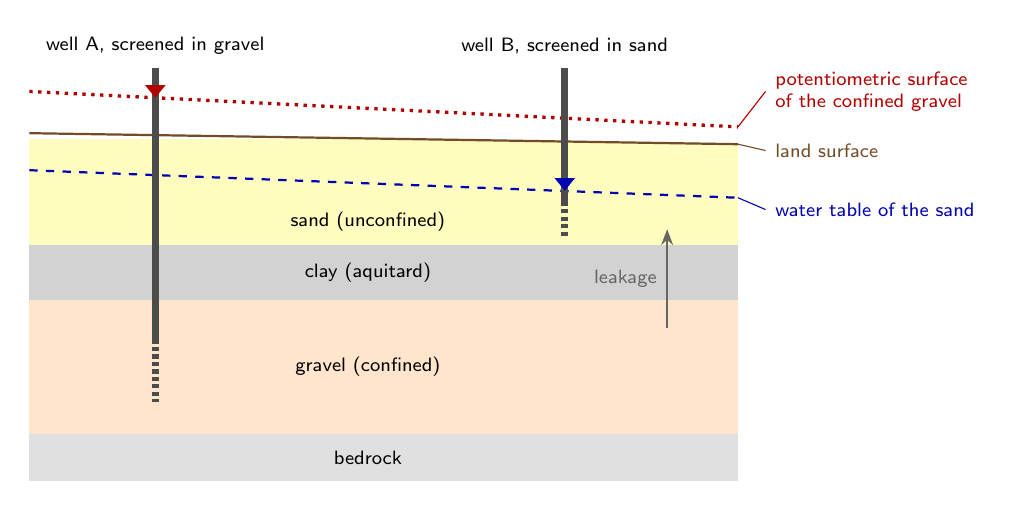
\begin{tikzpicture}[x=1cm,y=1cm,lab/.style={font=\scriptsize,align=center},leg/.style={font=\scriptsize,anchor=west,align=left}]
\fill[yellow!25] (0,3) rectangle (9,4.35); \fill[gray!35] (0,2.3) rectangle (9,3);
\fill[orange!20] (0,0.6) rectangle (9,2.3); \fill[black!12] (0,0) rectangle (9,0.6);
\fill[white] (0,4.42) -- (9,4.28) -- (9,4.4) -- (0,4.5) -- cycle;
\draw[thick,brown!60!black] (0,4.42) -- (9,4.28);
\draw[dotted,red!70!black,very thick] (0,4.95) -- (9,4.5);
\draw[dashed,blue!70!black,thick] (0,3.95) -- (9,3.6);
\node[lab] at (4.3,3.3) {sand (unconfined)}; \node[lab] at (4.3,2.65) {clay (aquitard)};
\node[lab] at (4.3,1.45) {gravel (confined)}; \node[lab] at (4.3,0.3) {bedrock};
\draw[line width=2.5pt,black!70] (1.6,5.25) -- (1.6,1.8); \draw[line width=2.5pt,black!70,dash pattern=on 1.5pt off 1.2pt] (1.6,1.8) -- (1.6,1.0);
\fill[red!70!black] (1.6,4.87) -- ++(-0.13,0.16) -- ++(0.26,0) -- cycle;
\node[lab,anchor=south] at (1.6,5.3) {well A, screened in gravel};
\draw[line width=2.5pt,black!70] (6.8,5.25) -- (6.8,3.55); \draw[line width=2.5pt,black!70,dash pattern=on 1.5pt off 1.2pt] (6.8,3.55) -- (6.8,3.1);
\fill[blue!70!black] (6.8,3.69) -- ++(-0.13,0.16) -- ++(0.26,0) -- cycle;
\node[lab,anchor=south] at (6.8,5.3) {well B, screened in sand};
\draw[-{Stealth[length=2mm]},thick,black!60] (8.1,1.95) -- node[lab,left]{leakage} (8.1,3.2);
\draw[red!70!black] (9,4.5) -- (9.35,4.95) node[leg] {potentiometric surface\\ of the confined gravel};
\draw[brown!60!black] (9,4.28) -- (9.35,4.2) node[leg] {land surface};
\draw[blue!70!black] (9,3.6) -- (9.35,3.45) node[leg] {water table of the sand};
\end{tikzpicture}

\caption{The same place can have two different heads: the water table of the upper sand and the higher potentiometric surface of
the confined gravel below the clay. Water leaks upward through the clay because the gravel head is higher.}\label{fig:potsurf}
\end{figure}
\section{Three kinds of boundary conditions}
\begin{table}[!htbp]\centering
\caption{Three kinds of boundary conditions.}
\begin{tabular}{P{0.22\linewidth}P{0.368\linewidth}P{0.34\linewidth}}\toprule\hdr
Kind & Meaning & In this coupling\\\midrule
Specified flow & the flow is known (it does not depend on the head) & recharge, wells, reservoir seepage\\
Specified head & the head is known; the flow is whatever is needed & fixed-head boundaries (CHD)\\
Head-dependent flow & flow = conductance $\times$ (boundary level $-$ head) & rivers, seepage drains, wetlands, lakes, general-head boundaries, water-table ET\\\bottomrule
\end{tabular}
\end{table}
Head-dependent boundaries are the heart of a coupled model: they let the aquifer and the surface water ``negotiate'' the
exchange according to the water levels on both sides.

\section{The Newton method in simple terms}
The flow equations are non-linear: in an unconfined layer, transmissivity depends on the saturated thickness, which
depends on the unknown head. MODFLOW therefore solves them iteratively: guess heads, compute the imbalance of every cell,
correct the heads, and repeat until the corrections are smaller than a tolerance (here 0.00001 m, i.e.\ 0.01 mm). The Newton--Raphson method
computes each correction from the slope of the imbalance with respect to the heads, which converges quickly even when cells
are nearly dry. Each repetition is an \emph{outer iteration}; \cmd{GWBudget.csv} reports how many were needed each step
(typically 3--10 in the Liard example).

\section{A cell's water account, with numbers}
\begin{example}[: one cell for one day]
A 4 km$^2$ gravel cell receives 8\,000 m$^3$ recharge; it gets 1\,500 m$^3$ from an up-gradient neighbour and passes
2\,500 m$^3$ to a down-gradient one; its drain removes 4\,000 m$^3$. Inflow $-$ outflow $=8\,000+1\,500-2\,500-4\,000=3\,000$
m$^3$ are stored, so with $S_y=0.25$ the water table rises by $3\,000/(4\times10^6\times0.25)=3$ mm. MODFLOW finds heads for
which every cell's account balances like this one at the same time.
\end{example}

\section{Units and conversions}
\begin{table}[!htbp]\centering
\caption{Units and conversions.}
\begin{tabular}{P{0.44\linewidth}P{0.5\linewidth}}\toprule\hdr
Quantity & Conversion\\\midrule
depth of water in an HRU to volume & $V\,[\mathrm{m}^3]=x\,[\mathrm{mm}]\times A\,[\mathrm{km}^2]\times1000$\\
flow & 1 m$^3$/s $=86\,400$ m$^3$/d\\
recharge rate & 1 mm/d over 1 km$^2$ $=1\,000$ m$^3$/d\\
hydraulic conductivity & 1 m/d $\approx1.16\times10^{-5}$ m/s\\
leakance & conductance per area, d$^{-1}$; $C=\Lambda\times$area\\\bottomrule
\end{tabular}
\end{table}

\chapter{Building the groundwater model}\label{ch:c3}
Raven's HRUs are irregular areas; MODFLOW needs a regular three-dimensional grid. This chapter follows the model builder step by step. It shows which HRUs are coupled, how their polygons are placed on a map
and covered with a grid, and how much of each HRU falls in each cell. It then shows how the layers are built from the land
surface down to bedrock, which MODFLOW files are written, and how MODFLOW solves each step.

\section{From HRUs to a groundwater grid}\label{ch:grid}
\subsection{Which HRUs are coupled}
An HRU is \emph{coupled} when its \cmd{AQUIFER\_PROFILE} in the \cmd{.rvh} file names a profile defined in the
\cmd{.rvp} file. HRUs with \cmd{[NONE]} (or an empty entry) keep Raven's usual behaviour. Disabled HRUs are never
coupled (Raven prints a warning). We write $\mathcal{K}$ for the set of coupled HRUs and $a(k)$ for the aquifer profile of HRU $k$.

Raven checks two rules at start-up:
\begin{itemize}
\item No Raven process may take water \emph{out of} \cmd{GROUNDWATER} in a coupled HRU (MODFLOW owns that water);
Raven stops with an error naming the process.
\item If a process sends water \emph{into} \cmd{GROUNDWATER} in an \emph{uncoupled} HRU, that water leaves the model;
Raven warns so the user can restrict the process with \cmd{:-->Conditional}.
\end{itemize}

\subsection{Map projection}
The HRU polygons are read from a GeoJSON file. GeoJSON coordinates are longitude $\mathrm{lon}$ and latitude $\mathrm{lat}$ in
degrees, which cannot be used directly for areas and distances. Raven converts them to metres with the
\emph{Lambert azimuthal equal-area} projection \cite{snyder1987map}, centred on the average centroid
$(\mathrm{lon}_0,\mathrm{lat}_0)$ of the coupled HRUs, on a sphere of radius $R_\oplus=6\,371\,007.181$ m:
\begin{align}
\kappa &= \sqrt{\frac{2}{1+\sin\mathrm{lat}_0\sin\mathrm{lat}+\cos\mathrm{lat}_0\cos\mathrm{lat}\cos(\mathrm{lon}-\mathrm{lon}_0)}},\\
x &= R_\oplus\,\kappa\cos\mathrm{lat}\,\sin(\mathrm{lon}-\mathrm{lon}_0),\\
y &= R_\oplus\,\kappa\left[\cos\mathrm{lat}_0\sin\mathrm{lat}-\sin\mathrm{lat}_0\cos\mathrm{lat}\cos(\mathrm{lon}-\mathrm{lon}_0)\right].
\end{align}
The reverse conversion (for looking up map values at cell locations) is
\begin{align}
\rho&=\sqrt{x^2+y^2},\qquad c=2\arcsin\frac{\rho}{2R_\oplus},\\
\mathrm{lat}&=\arcsin\!\left(\cos c\sin\mathrm{lat}_0+\frac{y\sin c\cos\mathrm{lat}_0}{\rho}\right),\\
\mathrm{lon}&=\mathrm{lon}_0+\operatorname{atan2}\!\left(x\sin c,\;\rho\cos\mathrm{lat}_0\cos c-y\sin\mathrm{lat}_0\sin c\right).
\end{align}
\begin{plain}
This projection keeps areas correct, which is what matters for water volumes: one square kilometre on the map is one
square kilometre on the ground, anywhere in the model area.
\end{plain}
When the centroid longitudes span more than 180$^\circ$ as written, they are averaged across the antimeridian if that
gives them a smaller span (those west of 0 count 360$^\circ$ more), so that a model across longitude 180$^\circ$ is centred on it (HRUs at 179.998$^\circ$ and
$-179.998^\circ$ give $\mathrm{lon}_0=180^\circ$); the longitudes Raven derives are within $\pm180^\circ$, and a
longitude/latitude raster written beyond $\pm180^\circ$ across the antimeridian is sampled 360$^\circ$ east or west.

\subsection{The grid}
By default a square grid with cell size $\Delta$ (\cmd{:GridCellSize}, default 1\,000 m) covers the rectangle around all
coupled HRUs. Rows are numbered from north to south and columns from west to east. The plan-view cell (a whole column of
layers) is indexed $i$; its lower-left corner is $(x_0+c\Delta,\;y_0+(n_r-1-r)\Delta)$ for row $r$ and column $c$. Rotated
grids, grids refined around rivers and wells, quadtree grids, meshes that follow HRU boundaries and imported cells are
described in Section~\ref{sec:gridtypes}; everything below applies to all of them, with cell $i$ a polygon $\Omega_i$ of area $|\Omega_i|$.

\subsection{Polygon areas}
The area of a polygon with $N_v$ corners $(x_1,y_1),\dots,(x_{N_v},y_{N_v})$ is given by the shoelace formula
\begin{equation}
A=\tfrac12\sum_{v=1}^{N_v}\left(x_vy_{v+1}-x_{v+1}y_v\right),\qquad (x_{N_v+1},y_{N_v+1})=(x_1,y_1).
\end{equation}
The result is positive when the corners run counter-clockwise. Raven orients outer boundaries counter-clockwise and
holes clockwise, so the area of a polygon with holes is simply the sum over all its rings.
\begin{example}[: shoelace formula]
A square from $(0,0)$ to $(2,2)$ km: $\tfrac12[(0\cdot0-2\cdot0)+(2\cdot2-2\cdot0)+(2\cdot2-0\cdot2)+(0\cdot0-0\cdot2)]=\tfrac12(0+4+4+0)=4$ km$^2$.
\end{example}

\subsection{How much of each HRU lies in each cell}\label{sec:linkage}
For every HRU polygon $P_k$ and every cell $\Omega_i$ it touches, Raven cuts the polygon to the cell rectangle with
the Sutherland--Hodgman clipping algorithm \cite{sutherland1974clip} and measures the area of what remains:
\begin{equation}
A_{k,i}=\left|P_k\cap\Omega_i\right| .
\end{equation}
For rectangular cells (regular and quadtree grids) the polygon is clipped by the cell rectangle; for convex cells (HRU
meshes) by the cell polygon; a concave imported cell is split into triangles and clipped by each. The clipping works one
cell edge at a time: walking around the polygon, it keeps the corners that are inside the edge
and adds a new corner wherever the polygon crosses the edge. After four edges, what is left is the part of the polygon
inside the cell; the shoelace formula gives its area. (This gives the correct area even for concave polygons.)

\begin{example}[: overlap areas]
An HRU of 10 km$^2$ lies over three 2~km cells, covering 4.0, 3.5 and 2.5 km$^2$ of them. Its overlaps are
$A_{k,1}=4.0$, $A_{k,2}=3.5$, $A_{k,3}=2.5$ km$^2$, and the fractions of the HRU in each cell are 0.40, 0.35 and 0.25.
Every flow from this HRU to the grid is split 40/35/25.
\end{example}

\subsection{Active cells and their profile}
A column is \emph{active} when the coupled HRUs cover at least a fraction $f_{\min}$ (\cmd{:MinCellCoverage}, default
0.25) of it:
\begin{equation}
A^{\mathrm{cov}}_i=\sum_{k\in\mathcal{K}}A_{k,i}\ \ge\ f_{\min}\,|\Omega_i| .
\end{equation}
An active column takes the profile of the HRU with the largest overlap (the \emph{dominant} HRU),
$a(i)=a\!\left(\arg\max_k A_{k,i}\right)$. Fluxes still use the exact overlaps, so a column shared by two HRUs receives
water from both.

The table of overlaps $A_{k,i}$ over active columns is called the \emph{linkage}. It is the single source of truth for
moving water between HRUs and cells in both directions (Sections~\ref{ch:recharge}--\ref{ch:stores}).

\begin{watch}
The polygon area of an HRU need not equal its \cmd{AREA} in the \cmd{.rvh} file (Raven prints a warning when they
differ by more than 5\%). This does not break the water balance: volumes are always computed from the \cmd{.rvh} area
and split by overlap \emph{fractions}.
\end{watch}

\subsection{The linkage cache}
Computing the linkage requires reading and clipping every polygon. The result is saved in \cmd{<output>/mf6/linkage.cache}
(or the file named by \cmd{:LinkageCache}). The cache is labelled with a fingerprint (an FNV-1a hash) of the GeoJSON
file together with the ID field, the cell size and the list of coupled HRUs; if any of these change, Raven recomputes
the linkage. Numbers are written with 17 significant digits, so a run that reads the cache gives exactly the same
results as one that computed it.

\begin{figure}[!htbp]\centering
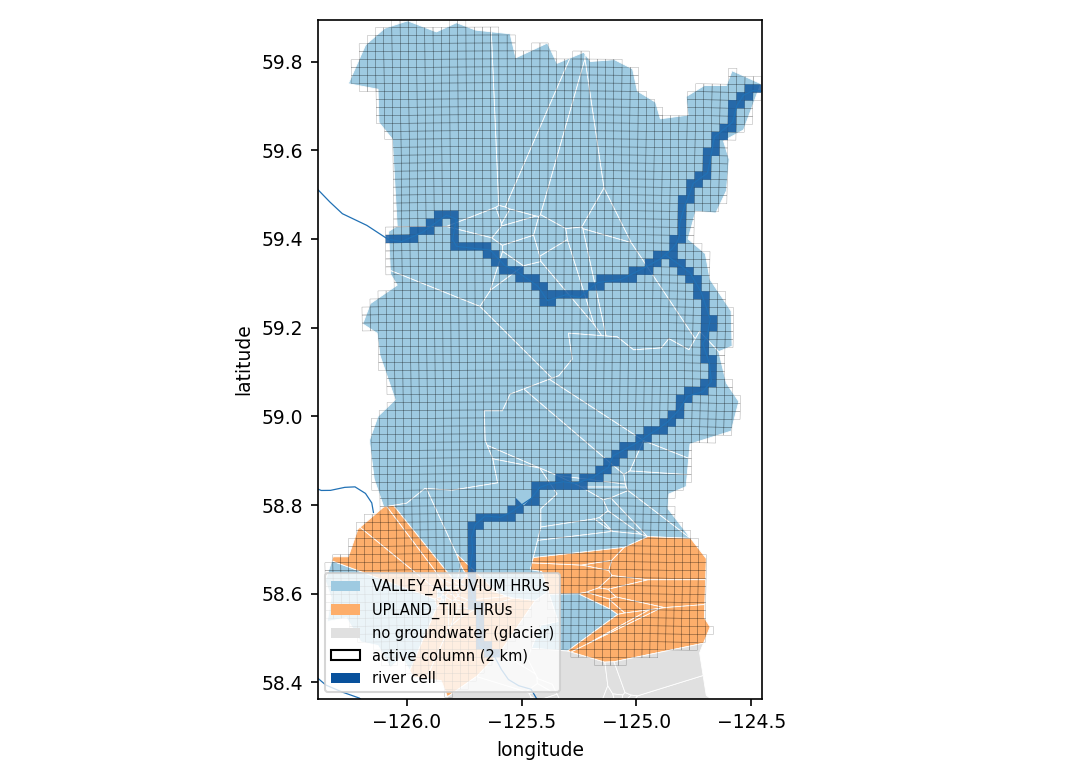
\includegraphics[width=0.9\linewidth]{figures/fig_grid_liard.png}
\caption{Liard example: coupled HRUs (colour = aquifer profile), active 2~km columns and river cells.}\label{fig:grid}
\end{figure}

\section{From one HRU to its cells: a complete example}
\begin{figure}[!htbp]\centering
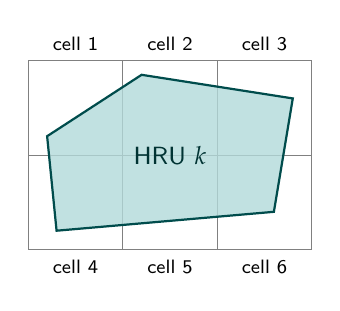
\begin{tikzpicture}[x=1.2cm,y=1.2cm]
\foreach \x in {0,1,2,3} \draw[gray] (\x,0) -- (\x,2);
\foreach \y in {0,1,2} \draw[gray] (0,\y) -- (3,\y);
\fill[teal!30,opacity=0.8] (0.3,0.2) -- (2.6,0.4) -- (2.8,1.6) -- (1.2,1.85) -- (0.2,1.2) -- cycle;
\draw[teal!60!black,thick] (0.3,0.2) -- (2.6,0.4) -- (2.8,1.6) -- (1.2,1.85) -- (0.2,1.2) -- cycle;
\node[font=\scriptsize] at (0.5,2.18) {cell 1}; \node[font=\scriptsize] at (1.5,2.18) {cell 2}; \node[font=\scriptsize] at (2.5,2.18) {cell 3};
\node[font=\scriptsize] at (0.5,-0.18) {cell 4}; \node[font=\scriptsize] at (1.5,-0.18) {cell 5}; \node[font=\scriptsize] at (2.5,-0.18) {cell 6};
\node[font=\small,teal!40!black] at (1.5,1.0) {HRU $k$};
\end{tikzpicture}
\caption{An HRU polygon over six grid cells. Clipping gives its area in each cell.}\label{fig:hrucells}
\end{figure}
\begin{example}[: an HRU through the whole chain]
Suppose the HRU in Figure~\ref{fig:hrucells} has an \cmd{.rvh} area of 3.2 km$^2$, 2 km cells, and clipping gives overlaps (km$^2$)
0.45, 0.55, 0.30 in cells 1--3 and 0.60, 0.85, 0.45 in cells 4--6 (sum 3.20).
\begin{enumerate}
\item \emph{Activation.} If other coupled HRUs fill the rest of these cells, all six have coverage above 25\% and are active.
\item \emph{Recharge.} Raven's percolation puts 1.5 mm into \cmd{GROUNDWATER}: $V=0.0015\times3.2\times10^6=4\,800$ m$^3$.
Cell 5 receives $4\,800\times0.85/3.20=1\,275$ m$^3$, i.e.\ $1\,275/4\times10^6=0.32$ mm over the whole cell (plus whatever other
HRUs deliver).
\item \emph{Seepage back.} If cell 5 seeps 10\,000 m$^3$ in the day and our HRU covers 0.85 of the 4 km$^2$ covered by all
HRUs in that cell, the HRU receives $10\,000\times0.85/4.0=2\,125$ m$^3$, i.e.\ $2\,125/3.2\times10^6\times1000=0.66$ mm in its lowest soil layer.
\item \emph{Water-table depth in the outputs.} \cmd{GWHRUState.csv} reports the overlap-weighted mean head of the six cells.
\end{enumerate}
\end{example}

\section{Preparing the geometry}
\subsection{What the HRU GeoJSON must contain}
A \cmd{FeatureCollection} of \cmd{Polygon} or \cmd{MultiPolygon} features in longitude/latitude (EPSG:4326), or in the
projection of \cmd{:InputCRS} (Section~\ref{sec:inputcrs}), each with a property holding the HRU ID of the \cmd{.rvh} file. Holes are allowed. Several features may share an ID (their areas add up).
\par\noindent\begin{minipage}{\linewidth}
\begin{lstlisting}
{"type":"FeatureCollection","features":[
 {"type":"Feature","properties":{"HRU_ID":2736},
  "geometry":{"type":"Polygon","coordinates":[[[-124.91,59.22],[-124.80,59.22],
              [-124.80,59.30],[-124.91,59.30],[-124.91,59.22]]]}} ]}
\end{lstlisting}
\end{minipage}\par\smallskip
Only HRUs with an \cmd{AQUIFER\_PROFILE} need polygons; others may be present and are ignored.
Every GeoJSON file Raven reads (HRUs, grids, boundaries, refinement features) is read as strict JSON: a coordinate must be a
finite JSON number: a string such as \cmd{"-124.91"}, \cmd{null}, \cmd{true}, \cmd{NaN} or \cmd{Infinity} stops the run,
naming the file, the feature, the ring and the vertex, and so does a position that is not an array of at least two
numbers (coordinates nested one level too deep or too shallow for the geometry type, a vertex \cmd{[1]}); hexadecimal
numbers and numbers with leading zeros are not JSON, and neither is text after the root object (the file is refused as
invalid JSON, naming the line and column). \cmd{NaN}, \cmd{Infinity} and \cmd{-Infinity} are read in the attributes, as
GDAL and Python's \cmd{json} write them, and \cmd{\textbackslash uXXXX} escapes are read as the characters they stand for,
so a field name such as \cmd{H\"ohe\_ID} matches. An ID field must hold a whole number, or a string that holds exactly
one (\cmd{7}, \cmd{7.0}, \cmd{"7"}, \cmd{" 7"}, \cmd{"7.0"}); \cmd{null}, \cmd{true}, a fraction or other text stops the run
(features of other geometry types than the file's are skipped before their ID is read), naming the file, the
feature and the value. A feature without a \cmd{"properties"} member stops the run where an ID field is read (a boundary
or refinement file needs none).
\subsection{Raster maps}\label{sec:rasters}
\cmd{:LandSurface} and \cmd{:BedrockSurface} take an ESRI ASCII grid or a GeoTIFF file (Section~\ref{sec:geotiff}), in
longitude/latitude or in the projection of \cmd{:InputCRS} (Section~\ref{sec:inputcrs}). An ESRI ASCII grid, for example:
\par\noindent\begin{minipage}{\linewidth}
\begin{lstlisting}
ncols 125
nrows 115
xllcorner -126.6
yllcorner 58.1
cellsize 0.02
NODATA_value -9999
 612.3 615.9 ...
\end{lstlisting}
\end{minipage}\par\smallskip
Values are interpolated bilinearly between raster cell centres, ignoring no-data cells; each model cell takes the mean of
$5\times5$ such samples. Points more than half a raster cell beyond the map's edge (one cell beyond the outermost cell centres) count as no-data. A grid without a
\cmd{NODATA\_value} line has no no-data value, as GDAL reads it: every number is an elevation (Raven warns when such a grid
holds $-9999$, which often marks missing data). The header keys may come in any order and case; \cmd{xllcenter} and
\cmd{yllcenter} give the centre of the lower-left cell instead of its corner; rectangular cells are given, as GDAL writes
them, by \cmd{dx} and \cmd{dy} instead of \cmd{cellsize}; \cmd{NODATA\_value nan} marks no-data cells written as
\cmd{nan}; a UTF-8 byte-order mark before the header and a DOS end-of-file mark (Ctrl-Z) after the values are ignored. The grid must hold exactly \cmd{ncols}$\times$\cmd{nrows} values: an unknown header key, a key given twice or both
\cmd{xllcorner} and \cmd{xllcenter} (or both \cmd{y} keys), a header value or a
cell value that is not a number, fewer values or more values (a wrong \cmd{ncols} would otherwise wrap the rows) stop
the run with a message naming the problem.

A raster that gives no value for any active column (all 25 samples of every column no-data or off the map) stops the run:
it is a map of another area, has a wrong corner, or is in another projection than \cmd{:InputCRS}. The message gives the
raster's extent and the extent of the active columns, both in the raster's coordinates. A raster that misses only some
columns gives a warning with their number; those columns take the area-weighted HRU \cmd{ELEVATION} (DEM) or lie
\cmd{DEFAULT\_BEDROCK\_DEPTH} below the land surface (bedrock). A raster may have at most 50 million cells: resample a
finer one (a few raster cells per model cell are enough).

\subsubsection{GeoTIFF files}\label{sec:geotiff}
A raster file whose name ends in \cmd{.tif}, \cmd{.tiff} or \cmd{.gtiff} (in any case) is read as GeoTIFF by Raven's own reader; no GDAL
or other library is needed. The values and their georeferencing are then sampled exactly as those of an ESRI ASCII grid:
a GeoTIFF and an ESRI ASCII grid with the same values give the same model.
\begin{center}
\begin{tabular}{P{0.25\linewidth}P{0.68\linewidth}}
\toprule\hdr Item & Supported\\\midrule
file & classic TIFF and BigTIFF, little- and big-endian; the first image of the file (overviews are ignored); at most 1~GB\\
units & coordinates in metres (projections) or degrees from Greenwich, elevations in metres: units keys, a projected code
in other units, a prime meridian (by code, by its longitude or by the datum), a vertical coordinate system in feet or a
band unit that is not a metre form (Table~\ref{tab:bandunits}) stop the run; a vertical system Raven does not know
gives a warning (read as metres)\\
scale and offset & GDAL's band \cmd{SCALE} and \cmd{OFFSET} (tag \cmd{GDAL\_METADATA}, items with GDAL's role
\cmd{scale}, \cmd{offset}, \cmd{unittype}; items of the same name without it are ordinary metadata, as for GDAL) are
applied, value $\times$ scale $+$ offset, as GDAL's \cmd{-unscale} and GIS programs show the values; no-data pixels, and
values beyond the range of a double, are no-data; a \cmd{GDAL\_METADATA} tag over 16~MB stops the run\\
side file & GDAL's side file \cmd{<raster>.aux.xml} (written for example with \cmd{-co PROFILE=GeoTIFF} or
\cmd{BASELINE}, or when metadata are set on a file opened read-only) is read as GDAL reads it, before the file's own
metadata: in its \cmd{PAMRasterBand band="1"}, a \cmd{Scale} or an \cmd{Offset} replaces both of the file's (the other
is then 1 or 0), a \cmd{UnitType} replaces the band unit, and a \cmd{NoDataValue} replaces \cmd{GDAL\_NODATA}. Raven reads
the side file, and \cmd{GDAL\_METADATA}, only in the form GDAL writes them (its layout, attributes in double quotes, one
\cmd{PAMRasterBand} per band, GDAL's escapes, and the comments, literals such as \cmd{<!DOCTYPE ...>}, processing
instructions and mixed text GDAL writes in an \cmd{xml:} metadata domain, which are read past); one in any other form that names a band or a band value (\cmd{PAMRasterBand},
\cmd{Scale}, \cmd{Offset}, \cmd{UnitType}, \cmd{NoDataValue}) stops the run (``rewrite it with GDAL'': \cmd{gdal\_translate}
or \cmd{gdal\_edit.py}), and one that names none is ignored, as GDAL takes no band value from it; a file with CRLF line ends is not
in that form (the message says so); a GeoTIFF's side file that holds georeferencing (\cmd{GeoTransform}, \cmd{SRS} or \cmd{GCPList},
which GDAL may take in place of the raster's own), a value that is not a number or a side file over 16~MB stops the run. An ESRI ASCII grid's side file is read the same way (its \cmd{Scale},
\cmd{Offset} and \cmd{UnitType}; GDAL keeps the grid's \cmd{NODATA\_value}, and ignores a \cmd{GeoTransform} or \cmd{SRS} there, taking
the grid's header and its \cmd{.prj}, as Raven does), so a GeoTIFF and the ESRI ASCII grid GDAL makes
of it give the same model. Georeferencing kept only in the side file (\cmd{BASELINE}) is not read: such a file stops as having no georeferencing\\
layout & strips or tiles\\
compression & none, LZW, DEFLATE (codes 8 and 32946) and PackBits\\
predictor & none, horizontal differencing (2) and floating-point (3), with LZW and DEFLATE\\
values & one band (one sample per pixel, grey scale); unsigned and signed integers of 8, 16, 32 and 64 bits, floating
point of 32 and 64 bits\\
georeferencing & north-up: \cmd{ModelPixelScale} with \cmd{ModelTiepoint}, or a \cmd{ModelTransformation} without rotation
or shear; pixels may be rectangular\\
pixel position & \cmd{PixelIsArea} (the default): the tie point is the corner of the pixel; \cmd{PixelIsPoint}: the tie
point is the centre of the pixel, so the raster's corner lies half a pixel up and left of it (as GDAL reads it)\\
no-data & the \cmd{GDAL\_NODATA} tag (a 32-bit float raster compares at 32-bit precision; \cmd{nan} allowed), and a GDAL
internal mask (1 or 8 bits; mask 0 is no-data; looked for among the first 4\,096 image directories; a damaged
chain of directories after the raster gives a warning and the raster without its mask); without either every value is valid, as GDAL reads it. NaN and infinite
values are always no-data\\
\bottomrule
\end{tabular}
\end{center}
The run stops with a message naming the file and the reason for: other compressions (JPEG, ZSTD, LZMA, LERC, WebP,
\dots), more than one band, a palette or colour image, other bit depths (1, 12 or 16-bit floating point, complex values),
a rotated, sheared or south-up raster, control points without a pixel size, no georeferencing, geocentric coordinates,
bits stored in reverse order (\cmd{FillOrder} 2), projected coordinates or elevations in other units than metres
(\cmd{ProjLinearUnitsGeoKey}, \cmd{GeogLinearUnitsGeoKey}, \cmd{VerticalUnitsGeoKey}) or longitude/latitude in other units
than degrees, a geographic code or key with a prime meridian other than Greenwich (for example EPSG:4801, Bern), also
when the prime meridian is given only by its longitude (\cmd{GeogPrimeMeridianLongGeoKey}, as GDAL writes a user-defined
longitude/latitude system such as \cmd{+pm=paris}) or by the datum (\cmd{GeogGeodeticDatumGeoKey}, for example 6801), a
projected code whose coordinates are in feet or other units when the file has no \cmd{ProjLinearUnitsGeoKey} (for example
EPSG:2227, California zone 3 in US survey feet), a band unit (\cmd{UNITTYPE} in \cmd{GDAL\_METADATA}, or
\cmd{UnitType} in the side file) that is not a metre form, a band \cmd{SCALE} of 0, a
vertical coordinate system in feet (for example EPSG:4269+6360, NAVD88 in US survey feet), an internal mask Raven cannot
read, a truncated or corrupt file or a decompression error, and a file over 1~GB, 50 million pixels, or strips or tiles
covering more than 200 million pixels. Raven is stricter than GDAL in a few rare cases: a negative pixel height
(\cmd{ModelPixelScale}, which GDAL reads north-up by default) is refused, a \cmd{ModelTiepoint} tag of more than 4\,096
values is taken as no georeferencing, and a \cmd{GDAL\_NODATA} text longer than 256 characters is ignored.

\paragraph{Band unit.} GDAL's band unit (\cmd{UNITTYPE} in \cmd{GDAL\_METADATA}, or \cmd{UnitType} in the side file;
set with \cmd{gdal\_edit.py -units}) is free text, so Raven's rule is closed: the raster is read as metres only when the
whole text, normalised, is a metre form of Table~\ref{tab:bandunits}: a metre word, symbol or abbreviation, alone or followed
by one listed vertical datum (\cmd{m MSL}, \cmd{m, AHD}, \cmd{m (NAVD88)}, \cmd{m(NAVD88)}, \cmd{m-NAVD88},
\cmd{m NAVD88 GEOID18}, \cmd{meters (EGM2008 geoid)}, \cmd{m above sea level}, fused \cmd{mAHD}, \cmd{msnm}, \cmd{m.s.n.m.}), a metre form in brackets after a metre word (\cmd{meter (m)},
\cmd{metre (EPSG:9001)}), or a metre form after a quantity, in brackets or after \cmd{in} (\cmd{elevation (m)},
\cmd{Elevation [m]}, \cmd{height in metres}, \cmd{height above ellipsoid (m)}, \cmd{H\"ohe (m)}, \cmd{Elevation\_m}). Normalising reads full-width characters as
ASCII and no-break and ideographic spaces as blanks, trims the blanks and reads a run of them as one, lowers the case (ASCII,
Latin-1, Latin Extended-A, Greek, whose accents are also removed, and Cyrillic) and removes surrounding brackets: \cmd{m},
\cmd{m.}, \cmd{(m)}, \cmd{[metres]}, \cmd{Meters}, \cmd{MASL}, \cmd{m a.s.l.}, \cmd{m\"uNN}, \cmd{Meter \"uber NN},
\cmd{$\mu\acute{\epsilon}\tau\rho\alpha$}, the same in capitals without accents, a full-width \cmd{m}, \cmd{EPSG:9001} are
metres. A raster without a band unit is read as metres (empty brackets, \cmd{()} or \cmd{[]}, are a text). Any other text
stops the run with a message that names the text (bytes that are not UTF-8 shown as \cmd{\textbackslash xNN}), of one of
three kinds:
\begin{itemize}
\item a text with another length unit and no metre (the second row of the table: \cmd{ft}, \cmd{US survey foot},
\cmd{Zentimeter}, \cmd{km}, \cmd{EPSG:9002}, also \cmd{EPSG 9002} and \cmd{EPSG: 9003}, feet fused with a datum such as
\cmd{ftMSL}, \cmd{ftNAVD88} or \cmd{usftNGVD29}, the ESRI unit names \cmd{Link\_Clarke} or \cmd{Rod\_US}), or another length named with its metre conversion (\cmd{ft (0.3048 m)}, \cmd{M (feet)}): ``its elevations are
in \dots''; convert the values to metres and set the unit
(\cmd{gdal\_calc.py}, then \cmd{gdal\_edit.py -units m});
\item a scaled metre: a part or multiple (\cmd{m (in thousands)}, \cmd{tenths of a metre}, \cmd{m (in 1000s)}), a number with a
factor sign or word (\cmd{m*0.1}, \cmd{Meter (x0.1)}, \cmd{m (scaled by 0.1)}, \cmd{0.1 of a metre}, \cmd{Meter (Faktor 0,1)},
\cmd{units of 0.1 m}, \cmd{m\^{}2}), a power of ten or an ordinal (\cmd{m 1e-2}, \cmd{m E-2}, \cmd{100ths of a metre}), or a number
and a metre form as the whole text (\cmd{0.1 m}, \cmd{1000 m}, \cmd{1e-2 m}, \cmd{.1 m}): the values are not plain metres; write them unscaled, or give
the scale as the band's scale and offset (\cmd{gdal\_edit.py -scale 0.1 -units m});
\item any other text (\cmd{m (Admiralty datum)}, \cmd{hydraulic head}, \cmd{m/s}, \cmd{5 km grid, elevation in m}, \cmd{m
(NAVD 1988)}): if the elevations are in metres (after the band scale and offset), state it by writing \cmd{METRES} (or
\cmd{METERS}) after the file name, otherwise convert as above:
\begin{verbatim}
:LandSurface   dem.tif   METRES
\end{verbatim}
(\cmd{:BedrockSurface} likewise).
\end{itemize}
\cmd{METRES} is the user's statement that the values are metres, for a text Raven cannot place: it does not lift the
first two kinds (a recognised other length or scaled metre stops also with it). With \cmd{METRES} every run writes a
warning that names the file's own unit text, also for a metre form or no unit (``read as metres because METRES follows the
file name \dots; the file's own band unit is \dots''), so that a wrong statement shows.
\begin{table}[!htbp]\centering
\caption{Band units: the metre forms read as metres (with their datums and quantities), and the other lengths named in the stop message.}\label{tab:bandunits}\small
\begin{tabularx}{\linewidth}{P{0.2\linewidth}Y}\toprule\hdr
Class & Forms (the whole text, normalised)\\\midrule
metre (read as metres) & the metre written out: \cmd{metre}, \cmd{metres}, \cmd{meter}, \cmd{meters}, \cmd{metern},
\cmd{m\`etre(s)}, \cmd{m\'eter}, \cmd{m\'eterben}, \cmd{metro(s)}, \cmd{metri}, \cmd{metr}, \cmd{metra}, \cmd{metry},
\cmd{metr\'ow}, \cmd{metrach}, \cmd{metrami}, \cmd{metrze}, \cmd{metrem}, \cmd{metr\r{u}}, \cmd{metrech}, \cmd{metru},
\cmd{metrin}, \cmd{metri\"a}, \cmd{metrit}, the metre in Cyrillic (with its endings), Greek, Chinese,
Japanese and Korean; the symbol \cmd{m} (also its Cyrillic letter); \cmd{masl}, \cmd{m asl},
\cmd{m a.s.l.}, \cmd{m.a.s.l.}, \cmd{mamsl}, \cmd{m amsl}, \cmd{m a.m.s.l.}, \cmd{moh}, \cmd{m.o.h.}, \cmd{m\"oh},
\cmd{m \"o.h.}, \cmd{m.\"o.h.}, \cmd{m o.h.}, \cmd{mt}, \cmd{mts}, \cmd{mtr}, \cmd{mtrs}, \cmd{m\"u}, \cmd{m\"uNN}, \cmd{m \"u. NN}, \cmd{m \"u.NN}, \cmd{m \"u. M.}, \cmd{m \"u.M.}, \cmd{m.}, and the Cyrillic metre of the
Baltic system (m BS, written together or apart); \cmd{EPSG:9001}, \cmd{EPSG::9001}, \cmd{EPSG 9001}, \cmd{urn:ogc:def:uom:EPSG::9001}, \cmd{http://www.opengis.net/def/uom/EPSG/0/9001}\\
vertical datums (after a metre form, also with a comma, \cmd{;}, \cmd{/}, \cmd{-} or \cmd{\_}, in brackets, or fused to \cmd{m} or \cmd{m.}) & \cmd{MSL}, \cmd{AMSL},
\cmd{ASL}, \cmd{a.s.l.}, \cmd{a.m.s.l.}, \cmd{above sea level}, \cmd{above mean sea level}, \cmd{AHD}, \cmd{AOD}, \cmd{ODN},
\cmd{NAP}, \cmd{+NAP}, \cmd{TAW}, \cmd{NN}, \cmd{NHN}, \cmd{\"u. NN}, \cmd{\"u.NN}, \cmd{\"uber NN}, \cmd{\"u. NHN},
\cmd{\"u.NHN}, \cmd{\"uber NHN}, \cmd{\"u. M.}, \cmd{NN2000}, \cmd{RH2000}, \cmd{DVR90}, \cmd{NAVD88}, \cmd{NAVD 88},
\cmd{NGVD29}, \cmd{NGVD 29}, \cmd{CGVD2013}, \cmd{CGVD28}, \cmd{EGM96}, \cmd{EGM2008}, \cmd{s.l.m.}, \cmd{slm},
\cmd{n.p.m.}, \cmd{npm}, \cmd{s.n.m.}, \cmd{snm}, \cmd{n. m.}, \cmd{n.m.}, \cmd{ellipsoidal}, \cmd{above (the) ellipsoid};
\cmd{s. n. m.}, \cmd{EGM08}, \cmd{OD}, \cmd{MLLW}, \cmd{MLW}, \cmd{MHW}, \cmd{MHHW}, \cmd{LAT}, \cmd{HAE}, \cmd{orthometric},
\cmd{NGF}, \cmd{IGN69}, \cmd{N2000}, \cmd{NZVD2016}, \cmd{T.P.}, \cmd{(the) WGS84 ellipsoid}; \cmd{NAVD}, \cmd{NGVD},
\cmd{EVRF2000}, \cmd{EVRF2007}, \cmd{DHHN92}, \cmd{DHHN2016}, \cmd{NHN2016}, \cmd{\"u. NHN2016}, \cmd{LN02}, \cmd{\"u. A.},
\cmd{Bpv}, \cmd{n. m. Bpv}, \cmd{NGF-IGN69}, \cmd{t.o.v. NAP}, \cmd{N60}, \cmd{DNN}, \cmd{AHD71}, \cmd{CD}, \cmd{chart datum},
\cmd{OSGM15}, \cmd{Ordnance Datum}, \cmd{geoid}, \cmd{WGS84}, \cmd{TP}; each may end in \cmd{geoid} or a geoid model
(\cmd{m NAVD88 GEOID18}, \cmd{m NAVD88 (GEOID12B)}), follow \cmd{above} or \cmd{over} (\cmd{m above MSL}) and have a blank before its year (\cmd{RH 2000}, \cmd{EGM 96}); a dotted abbreviation of a
metre form or datum may lack its final dot (\cmd{m a.s.l}, \cmd{moh.} with it)\\
quantities (before a metre form in brackets or after \cmd{in}) & \cmd{elevation(s)}, \cmd{height(s)}, \cmd{altitude},
\cmd{elevation / height above (mean) sea level}, \cmd{height above ellipsoid}, \cmd{height\_above\_ellipsoid},
\cmd{ellipsoidal height}, \cmd{orthometric height}, \cmd{elev}, \cmd{z}, \cmd{DEM}, \cmd{DTM}, \cmd{DSM}, and in the languages
of the metre words \cmd{H\"ohe}, \cmd{altitud}, \cmd{altura}, \cmd{cota}, \cmd{hauteur}, \cmd{\'el\'evation}, \cmd{quota},
\cmd{altezza}, \cmd{altitudine}, \cmd{hoogte}, \cmd{wysoko\'s\'c}, \cmd{v\'y\v{s}ka}, \cmd{nadmo\v{r}sk\'a v\'y\v{s}ka},
\cmd{magass\'ag}, \cmd{korkeus}, \cmd{h\"ojd}, \cmd{h\o{}yde}, \cmd{h\o{}jde}, \cmd{\^in\u{a}l\c{t}ime}, the height in Cyrillic and Greek;
also before a comma (\cmd{Elevation, m}) or joined by \cmd{\_} (\cmd{Elevation\_m})\\
another length (named in the message; \cmd{METRES} does not apply) & a text with one of these and no metre form among its
words: feet, inches, yards, miles, fathoms, chains and furlongs in English and other languages and case forms (\cmd{ft},
\cmd{foot}, \cmd{feet}, \cmd{fasl}, \cmd{inch(es)}, \cmd{yard(s)}, \cmd{mile(s)}, \cmd{pie(s)}, \cmd{pied(s)}, \cmd{voet},
\cmd{Fu\ss}, \cmd{F\"u\ss e}, \cmd{stopa}, \cmd{stopach}, \cmd{st\'op}, \cmd{jalka}, \cmd{l\'ab}, \cmd{l\'abban}, \cmd{Zoll},
\cmd{pulgada(s)}, \cmd{Meile(n)}, \cmd{polegada(s)}, \cmd{milha(s)}, \cmd{jarda(s)}, \cmd{cal}, \cmd{cale}, \cmd{mil},
\cmd{jardy}, \cmd{palce}, \cmd{m\'ile}, \cmd{h\"uvelyk}, \cmd{m\'erf\"old}, \cmd{tuuma}, \cmd{maili}, \cmd{jaardi}, \cmd{tum},
\cmd{tomme}, \cmd{picior}, \cmd{inci}, \cmd{yarzi}, \cmd{milles}, \cmd{verges}, \cmd{iarde}, \cmd{vara(s)}, the fathom as
\cmd{braza(s)}, \cmd{bra\c{c}a(s)}, \cmd{brasse(s)}, \cmd{toise(s)}, \cmd{Faden}, \cmd{Klafter}, \cmd{vadem}, \cmd{famn},
\cmd{favn}, and in Cyrillic, Greek, Chinese, Japanese and Korean, with the verst and arshin and the Chinese and Japanese
chi, shi chi, cun, zhang, li and ken); \cmd{micron(s)}, \cmd{rod(s)}, \cmd{perch(es)}, \cmd{league(s)},
\cmd{kft}; the ESRI unit names \cmd{Link\_}\dots, \cmd{Chain\_}\dots, \cmd{Rod\_}\dots; feet fused with a qualifier
(\cmd{ftUS}, \cmd{usft}, \cmd{SurveyFeet}) or a datum, its year kept (\cmd{ftMSL}, \cmd{ftNAVD88}, \cmd{ftNAVD 88},
\cmd{usftNGVD29}, also as a word of a longer text: \cmd{elevation (ftNAVD88)}); the metre's multiples and parts as symbols (\cmd{km}, \cmd{cm}, \cmd{mm},
\cmd{dm}, \cmd{nm}, \cmd{$\mu$m}, also Cyrillic) or with an SI prefix joined to a metre word or right before one
(\cmd{kilometres}, \cmd{Kilo Meter}, \cmd{Zentimeter}, \cmd{dec\'imetros}, \cmd{quil\'ometros}, \cmd{milli-metres}, and
the prefixed metres of Chinese, Japanese and Korean, also with a blank between the prefix and the metre);
\cmd{in}, \cmd{ch}, \cmd{mi}, \cmd{fath}, \cmd{link(s)}, \cmd{dam}, \cmd{hm} as the whole text (or after \cmd{us},
\cmd{ind}, \cmd{int}, \cmd{intl}); EPSG length codes other than 9001 as the whole text (\cmd{EPSG:9002},
\cmd{urn:ogc:def:uom:EPSG::9036}; as part of a longer text such codes, several of which also name coordinate systems,
are not read as units)\\\bottomrule
\end{tabularx}
\end{table}

A GeoTIFF without \cmd{GDAL\_NODATA} (for example one converted from an ESRI ASCII grid without its \cmd{NODATA\_value})
holds no no-data value: every value is an elevation, also $-9999$. When such a file holds $-9999$, the lowest or highest
32- or 64-bit float or, for signed integers, the type's minimum, Raven warns with the number of pixels of each value; if
they mark missing data, declare the no-data value (\cmd{gdal\_translate -a\_nodata -9999 in.tif out.tif}). A GeoTIFF that GDAL
writes with its default options (\cmd{gdal\_translate}, \cmd{gdalwarp}, QGIS export), uncompressed or with
\cmd{COMPRESS=LZW}, \cmd{DEFLATE} or \cmd{PACKBITS}, is read as it is; otherwise convert it, for example
\cmd{gdal\_translate -b 1 -co COMPRESS=DEFLATE in.tif dem.tif}.

\paragraph{Coordinate system of a GeoTIFF.} The EPSG code of the GeoTIFF keys (\cmd{ProjectedCSTypeGeoKey} of a projected
raster, \cmd{GeographicTypeGeoKey} of a geographic one) is checked against the run:
\begin{itemize}
\item a geographic code (longitude/latitude, any datum) is accepted without \cmd{:InputCRS} and refused with it;
\item a projected code needs \cmd{:InputCRS}: the same code, or a built-in code or parameters giving the same projection;
another built-in projection, or another EPSG code given as \cmd{:InputCRS}, is refused;
\item a projected code that is not built in cannot be compared with \cmd{:InputCRS} given by its parameters (\cmd{TMERC},
\cmd{ALBERS}, \cmd{LCC}): the file is read in the \cmd{:InputCRS} coordinates, with a warning; under \cmd{:InputCRS}
given as a code (\cmd{EPSG:}\emph{n} or \cmd{ESRI:102001}) it is refused. Without \cmd{:InputCRS} the message asks for
\cmd{:InputCRS EPSG:}\emph{n} when the code is built in, otherwise for the projection's parameters;
\item a user-defined coordinate system (code 32767) or none at all says nothing: the file is treated as an ESRI ASCII grid,
whose extent alone is checked (the longitude/latitude range without \cmd{:InputCRS}, ``looks like longitude/latitude''
with it).
\end{itemize}
The message of a refused file names the file, the code found and the coordinate system expected.
\subsection{Projected input files (\texttt{:InputCRS})}\label{sec:inputcrs}
Most GIS data are projected (UTM, Albers, Lambert). Instead of reprojecting them to longitude/latitude, give their
projection once in the \cmd{.rvg} file:
\begin{lstlisting}
:InputCRS EPSG:32610                                   # UTM zone 10 N (WGS84)
:InputCRS ALBERS 50 58.5 45 -126 1000000 0 GRS80       # or by parameters (here BC Albers, EPSG:3005)
\end{lstlisting}
The grammar is that of \cmd{:MF6CRS} (Section~\ref{sec:mf6crs}): the EPSG codes 326xx and 327xx (UTM, WGS84), 269xx (UTM, NAD83),
3005, 5070, 3978, 3347 and ESRI:102001, or \cmd{TMERC}, \cmd{ALBERS} and \cmd{LCC} by their parameters, on the WGS84 or GRS80
ellipsoid. The parameters are read strictly: each must be a plain number (\cmd{-ll7}, \cmd{O.9996} or \cmd{500km} stop
the run, naming the parameter), \cmd{TMERC} takes exactly five of them and \cmd{ALBERS} and \cmd{LCC} six, then at most
the ellipsoid, and an EPSG code takes nothing after it; latitudes must lie within $\pm90^\circ$ and $k_0$ must be
positive. \cmd{ALBERS} and \cmd{LCC} need a cone: standard parallels symmetric about the equator (\cmd{30 -30}, or
\cmd{0 0}) and, for \cmd{LCC}, a standard parallel at a pole stop the run, naming the parallels. The projection applies to every geometry and raster input file: \cmd{:HRUGeometry}, \cmd{:RiverGeometry},
\cmd{:GridFile}, the files of \cmd{:GridRefinement LINES} and \cmd{POLYGONS}, the boundary files of
\cmd{:GeneralHeadBoundary} and \cmd{:SpecifiedHeadBoundary}, \cmd{:LandSurface} and \cmd{:BedrockSurface} (also for the
soil zone's DEM samples), and for an existing model \cmd{:MF6GridFile}. Each vertex is converted to longitude/latitude as
it is read, and each raster is sampled in its own coordinates (the bilinear interpolation above, in metres), so a
projected DEM is used as it is, without resampling. Wells and monitoring wells may then be given by \cmd{X} and \cmd{Y}
(metres, in the same projection) instead of \cmd{LATITUDE} and \cmd{LONGITUDE}. Everything Raven writes stays in
longitude/latitude (\cmd{grid\_cells.geojson}, \cmd{GWHeads.nc}), and \cmd{GWModelSummary.txt} names the projection.

Input files whose coordinates do not match these settings are recognised where possible, and the run stops with a message:
\begin{itemize}
\item a GeoJSON file's \cmd{"crs"} member is read by the EPSG code that ends its name (\cmd{EPSG:32610}, as GDAL writes it
\cmd{urn:ogc:def:crs:EPSG::32610}, a versioned \cmd{urn:ogc:def:crs:EPSG:6.6:32610}, or
\cmd{http://www.opengis.net/def/crs/EPSG/0/32610}). A built-in projected code needs \cmd{:InputCRS} with that projection,
and a file whose code is another built-in projection than \cmd{:InputCRS} is refused. Geographic codes (longitude/latitude)
are accepted without \cmd{:InputCRS} and refused with it: the geographic 2D and 3D coordinate systems of the EPSG
registry, a table of 962 codes compiled into Raven (such as 4326 WGS\,84, 4979 WGS\,84 3D, 4269 NAD83, 4267 NAD27, 4617
NAD83(CSRS), 4258 ETRS89, 6318 NAD83(2011), 8255 NAD83(CSRS)v7, 7844 GDA2020), and OGC CRS84, CRS83 and CRS27. Codes
between 4000 and 4999 are not all geographic (4647, ETRS89 / UTM zone 32N, is a projection, as are 4087 and 4839). The
table also holds 69 geographic codes whose coordinates are not degrees from Greenwich (27 with another prime meridian,
such as 4801 Bern or 4807 NTF (Paris), and others in grads or degrees-minutes-seconds); a file in one of them is refused,
asking for a reprojection to EPSG:4326. A projected code whose coordinates are not metres (for example 2227, in US survey
feet; a table of 1\,016 codes) is refused too. A file that starts with a UTF-8 byte-order mark is read as any other. Any
other code cannot be classified: the file's coordinates decide, and without \cmd{:InputCRS} coordinates outside the
longitude/latitude range stop the run with a request for the projection's parameters (\cmd{TMERC}, \cmd{ALBERS} or
\cmd{LCC}); GeoTIFF rasters carry their code in their keys (Section~\ref{sec:geotiff});
\item without \cmd{:InputCRS}, a GeoJSON file with coordinates outside $\pm360^\circ$ / $\pm90^\circ$, or a raster whose
extent lies outside them, is refused (projected metres read as degrees);
\item with \cmd{:InputCRS}, a GeoJSON file or raster left in longitude/latitude is refused (``looks like
longitude/latitude''): its coordinates all lie within $\pm180^\circ$ / $\pm90^\circ$ and over the HRUs'
\cmd{LATITUDE}/\cmd{LONGITUDE} of the \cmd{.rvh} file, but not near the HRUs in the projection's coordinates (within
50~km plus half their extent);
\item a well given by \cmd{X} and \cmd{Y} needs \cmd{:InputCRS}.
\end{itemize}
A file without a \cmd{"crs"} member is taken to be in the projection of \cmd{:InputCRS} when it is given, so with
\cmd{:InputCRS} every input file must be projected (a projection given by its parameters, or a code not built in, cannot be
compared with a file's \cmd{"crs"} member and is accepted). The equal-area projection Raven lays its grid in
(Section~\ref{ch:grid}) is not changed by \cmd{:InputCRS}: the same HRU polygons given in longitude/latitude or in UTM give
the same grid and the same overlaps (within $10^{-9}$ of a cell area in the Liard test, Chapter~\ref{ch:verification}).
\subsection{Choosing the cell size}
The number of active columns is roughly the coupled area divided by $\Delta^2$: for the Liard example's 13\,000 km$^2$,
$\Delta=2$ km gives about 3\,300 columns, $\Delta=1$ km about 13\,000, $\Delta=500$ m about 52\,000. Run time grows roughly in
proportion. Choose $\Delta$ so that the narrowest valleys and the spacing of wells and monitoring wells span at least two or
three cells. The water balance is exact for any cell size (verified for 1, 2 and 4 km, Chapter~\ref{ch:verification}).

\section{Grid types}\label{sec:gridtypes}
\begin{plain}
The grid is the set of boxes (cells) in which MODFLOW calculates. By default Raven uses squares of one size. It can instead
turn the grid to follow a valley, use smaller cells near rivers and wells, shape the cells to follow your HRU boundaries, or
take cells made in another program. Smaller cells give more detail where it matters, at the cost of longer runs.
Figure~\ref{fig:grids} shows the same area on four grids.
\end{plain}
The grid need not be a regular array of squares. Five options cover most needs (Table~\ref{tab:gridtypes},
Figure~\ref{fig:grids}). All of them are built from the same inputs and keep the water accounts exact, and each can be
combined with every exchange, boundary, output and restart.

\begin{table}[!htbp]\centering
\caption{Grid options.}\label{tab:gridtypes}
\begin{tabularx}{\linewidth}{P{0.24\linewidth}P{0.13\linewidth}P{0.13\linewidth}Y}\toprule\hdr
Option & MODFLOW & XT3D default & Use it when\\\midrule
Regular (default) & DIS & no & a first model; uniform cells are enough\\
Regular, rotated and/or refined & DIS & no & a valley has a clear direction; finer cells near rivers or wells are wanted and whole rows and columns may be refined\\
\cmd{QUADTREE} & DISV & no & fine cells only where they matter (rivers, wells, areas of interest) with few cells elsewhere\\
\cmd{HRU\_MESH} & DISU & no & cells should follow HRU boundaries, so each cell belongs to one HRU\\
\cmd{FILE} (imported cells) & DISU & no & a grid made elsewhere (FloPy, gridgen, ModelMuse, QGIS) should be used\\
\cmd{:LayerConnection ELEVATION} (any grid) & DISU & no & layers of neighbouring profiles should connect where they are at the same elevation, not by layer number\\\bottomrule
\end{tabularx}
\end{table}

\begin{figure}[!htbp]\centering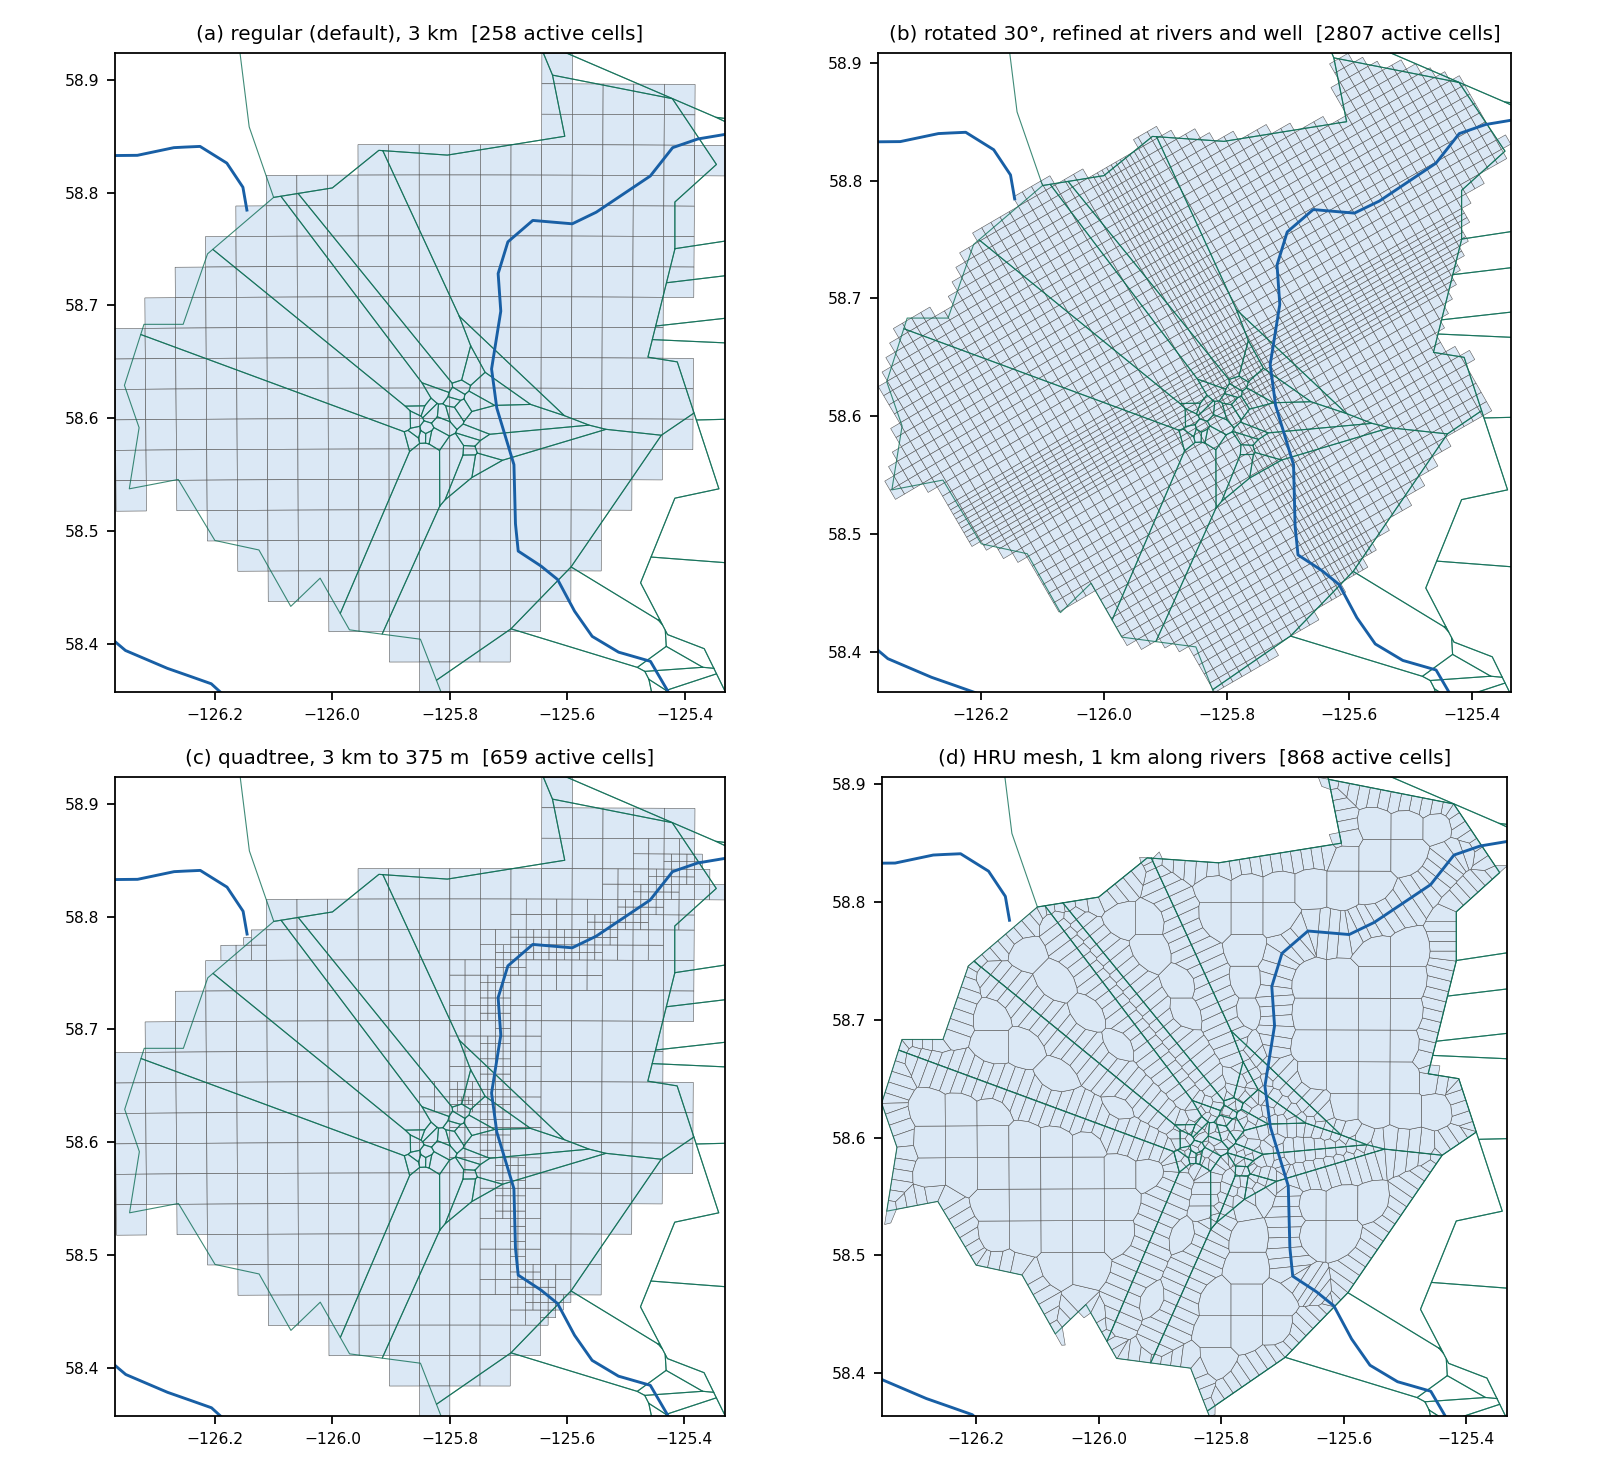
\includegraphics[width=0.78\linewidth]{figures/fig_grids.png}
\caption{The same model (Liard subbasin 52, HRU boundaries green, rivers blue) on four grids: (a) the default regular
grid; (b) rotated 30\textdegree{} and refined along rivers and around a well; (c) a quadtree refined along rivers and around the
well; (d) an HRU mesh whose cells follow HRU boundaries, with cells along the rivers.}\label{fig:grids}
\end{figure}

\subsection{Regular grids: rotation and variable spacing}
\cmd{:GridRotation} $\theta$ turns the grid $\theta$ degrees counterclockwise, for example to align columns with a valley.
The grid is built in its own rotated frame, in which every cell is still a rectangle; HRU polygons, rivers, wells and
boundaries are rotated into that frame, and MODFLOW receives the rotation as \cmd{ANGROT}. With \cmd{:GridRefinement} the grid gets variable spacing. Every base column and row that comes within the target size of a
refinement feature is divided into equal parts no larger than the target. Neighbouring columns and rows are then halved
until the widths change by at most a factor of two from one to the next. Refinement therefore always spans whole columns and rows.

\subsection{Quadtree grids}
A quadtree starts from large squares and cuts a square into four smaller ones wherever finer detail is wanted --- along a
river, say --- repeating until the cells are small enough. With \cmd{:GridType QUADTREE} a square is split into four while it is larger than the target size and a refinement feature
lies within half the target size of it. Splitting stops after \cmd{:QuadtreeMaxLevel} halvings (by default, enough to
reach the smallest target). The tree is then balanced so that neighbouring cells differ by one level at most. Where a large cell meets two
small ones its side carries the extra corner of the small cells (a hanging vertex), so MODFLOW's DISV input finds every
shared face. Because the line joining the centres of a large and a small cell is not perpendicular to their shared face,
MODFLOW's XT3D correction (the full conductance tensor) could be used. It is off by default, for two reasons found in the tests of Chapter~\ref{ch:verification}. The balanced quadtree was as
accurate without it (Thiem test). And XT3D --- even in its right-hand-side form --- slowed the Newton method badly where cells
dry and rewet: on the Liard model it took 32 instead of 7 iterations per day, and some days failed. \cmd{:FlowCorrection XT3D\_RHS} or \cmd{XT3D} switch it on.

\subsection{Meshes that follow HRU boundaries}
Picture a dot for every cell: each cell is the area closer to its own dot than to any other dot (a \emph{Voronoi} cell). If
two dots sit on opposite sides of an HRU boundary, at the same distance from it, the edge between their cells falls exactly
on that boundary. Raven places its dots this way, so the cells follow the HRU boundaries. In detail, with
\cmd{:GridType HRU\_MESH} the seed points are:
\begin{enumerate}
\item along every HRU boundary, pairs of seeds mirrored across the boundary at spacing $\delta_b=\min(\Delta/2,$ smallest
line refinement size (\cmd{RIVERS}, \cmd{LINES})$)$, or the \cmd{LAKES}/\cmd{POLYGONS} size where the boundary passes within
one such size of a refinement polygon, and $0.3\,\delta_b$ from it --- the face between the two seeds of a pair lies on the boundary;
\item seeds along refinement lines (rivers run through cell centres), in rings around refinement points (wells), and on a
staggered lattice of the target size inside and within one size around refinement polygons (lakes); seeds outside the
model's box (e.g.\ a monitoring well outside the model) are left out;
\item interior seeds on a lattice of spacing $\Delta$, kept only where no other seed is closer than about half the spacing.
\end{enumerate}
Each cell is the part of the plane closer to its seed than to any other. Raven builds it by cutting away, for each
neighbouring seed, the half of the plane that is closer to that neighbour. Each face remembers the seed on its other side, so
the connections between cells are exact. The line joining two seeds crosses their shared face at right angles, which is the
arrangement MODFLOW's standard method assumes, so no XT3D is needed. Where boundaries meet at sharp corners a cell may cover slivers of two HRUs. The overlaps are computed exactly, as for any
other grid, so the water accounts are unaffected. \cmd{GWModelSummary.txt} reports how much of each active cell's area lies
in its main HRU (typically above 99\%).

\subsection{Imported cells}
With \cmd{:GridType FILE} and \cmd{:GridFile cells.geojson ID\_FIELD} the cells are the polygons of a GeoJSON file in
longitude/latitude or in the projection of \cmd{:InputCRS}, one single-ring polygon per cell, numbered by the ID field (default \cmd{CELL\_ID}). Cells may be
concave, and a cell side may be shared with several smaller cells (T-junctions): neighbours are found wherever edges of two
cells lie on the same line --- within 0.1\% of the edge length, because a straight edge drawn in one map projection bends
slightly in another --- and overlap. A face made of several pieces gets their total length and their average position and
direction. Repeated vertices, which GIS exports often contain, are removed first. MODFLOW receives the grid as DISU with the
connection lengths, face widths and face directions computed from the polygons. Imported cells need not be orthogonal; for strongly non-orthogonal cells consider
\cmd{:FlowCorrection XT3D\_RHS} and check the convergence in \cmd{GWBudget.csv}.

\subsection{Connecting layers by elevation}\label{sec:layerconn}
In a layered grid a cell connects sideways only to the cell with the same layer number. When neighbouring columns have
different profiles --- a gravel layer thinning out next to a till, say --- the same layer number can mean different
materials at different elevations. \cmd{:LayerConnection ELEVATION} writes the grid as DISU and connects every pair of
cells of neighbouring columns whose vertical intervals overlap, as staggered horizontal connections (MODFLOW's \cmd{IHC}
2), so water flows between the layers that actually touch. Pass-through cells are removed and the cells above and below
them connected directly.

\subsection{Refinement}
\begin{lstlisting}
:GridRefinement RIVERS   250                     # along :RiverGeometry lines
:GridRefinement WELLS    100                     # around pumping and monitoring wells
:GridRefinement LAKES    250                     # in and around every reservoir's lake HRU
:GridRefinement LINES    faults.geojson    200   # along any lines
:GridRefinement POLYGONS wetlands.geojson  250   # inside and around polygons
\end{lstlisting}
Sizes must be smaller than \cmd{:GridCellSize}. Refinement applies to regular (variable spacing), quadtree and HRU-mesh
grids; an imported grid is used as it is. A grid is limited to 5 million cells per layer: a cell size or refinement that
gives more stops the run before the grid is built, naming the command and the number of cells. An imported grid
(\cmd{:GridType FILE}) with more cells stops naming the file, and an HRU mesh whose refinement makes more seeds stops
naming \cmd{:GridRefinement}; the cell size cannot help there. For a regular grid the
count is exact: the refined columns and rows are counted with the 2:1 smoothing that adds cells around each refined
strip, as the build makes them (test N24). For a quadtree it is estimated level by level from the squares the refinement features touch, each square
counted once however many features touch it (overlapping or adjacent features add no more), plus about a fifth for the
2:1 balance: 6\% below the cells built on the Liard example's grids, and between a third below and a fifth above on small
test grids of lines and polygons. So the estimate stops the run only beyond 1.5 times the limit; a grid nearer the limit
is built, and the build stops once it passes the limit. An HRU mesh is estimated before its seeds are placed (pairs along
the HRU boundaries, which take seeds at the smallest \cmd{LINES} or \cmd{RIVERS} size, seeds along the lines, around the
points and over the polygons, and the interior lattice); it stops beyond 1.5 times the limit, or when the boundary seeds
are so close for the cell size that building the cells would take more than a few minutes (seeds every 0.1~m along
65~km of HRU boundaries with 500~m cells, a size meant in kilometres). A grid within the limit that still needs more
memory than the computer has stops with a message naming the command and the estimated size.

\cmd{LAKES} needs no extra file: the outline of the lake HRU of every Raven reservoir (\cmd{:Reservoir \dots\ :HRUID}) is taken
from \cmd{:HRUGeometry}. Fine cells around a lake place its seepage (\cmd{:ReservoirExchange}) and the exchange along its shore
more precisely. On a regular grid the rows and columns through the lake are refined; a quadtree splits the squares in and
near the lake; an HRU mesh places cells of the target size inside the lake and in a band one cell wide around it, and
shortens the spacing of its cells along the shore. \cmd{POLYGONS} works the same way for any outline in a file.

\subsection{Rivers and boundaries on any grid}
On the default grid each segment of a river or boundary line is cut into pieces of at most a twentieth of the cell size,
and each piece goes to the cell that holds its middle. On every other grid each piece of a line is cut exactly at the edges of the cells it crosses (rectangles along their
sides, other cells along their edges or triangle by triangle). River lengths per cell are therefore exact and do not
depend on the cell size. A stretch lying exactly on a shared cell edge
is counted once. A boundary line may be drawn along the edge of the modelled area, where the edge cells can be inactive because too little
of them is covered. Such a line is attached to the nearest active cell within one cell size, so a boundary drawn on the
watershed outline is never lost.

\subsection{Choosing a grid}
Start with the default grid and a cell size of a few kilometres. Refine where heads and exchanges change quickly: along
rivers that gain or lose much water, around pumping wells, around lakes and reservoirs that leak to the aquifer, and in
wetlands. A quadtree gives the most accuracy per cell;
an HRU mesh gives the cleanest HRU--cell linkage; a rotated regular grid is simplest when a valley has one direction. XT3D
(\cmd{:FlowCorrection XT3D\_RHS} or \cmd{XT3D}) is off by default; use it only for strongly non-orthogonal imported cells, and
check that the model still converges well.

\subsection{Grid outputs}
Every run writes \cmd{mf6/grid\_cells.geojson}: each cell as a longitude/latitude polygon with its number (as in MODFLOW and in
the hotstart file), whether it is active, its profile, its dominant HRU and its area --- ready to be joined with heads in
QGIS. For grids other than regular, \cmd{GWHeads.nc} has a \cmd{cell} dimension instead of rows and columns, and the hotstart
block is written as \cmd{:GWHeads} \emph{nlay} \cmd{1} \emph{ncells}. The grid type, cell sizes, MODFLOW format and HRU
fidelity are reported in \cmd{GWModelSummary.txt}. Setting the environment variable \cmd{RAVEN\_GW\_PROFILE=1} prints the time
taken by each stage of building the model, useful for large grids.

\section{Building the layers}\label{ch:layers}
\subsection{Land surface, model top and bedrock}
For each active column Raven needs three elevations:
\begin{description}
\item[Land surface] $z_{\mathrm{land},i}$: the average of 25 points ($5\times5$) of the DEM over the cell
(\cmd{:LandSurface}); without a DEM, the area-weighted \cmd{ELEVATION} of the HRUs in the cell.
\item[Model top] $z_{\mathrm{top},i}=z_{\mathrm{land},i}-d_{\mathrm{sz},a}$, where $d_{\mathrm{sz},a}$ is the
\cmd{SOIL\_ZONE\_DEPTH} of the column's profile $a=a(i)$ (default 0, so the top is the land surface). With the soil-zone
coupling (\cmd{:SoilZone PHYSICAL}, Section~\ref{ch:soilzone}) \cmd{SOIL\_ZONE\_DEPTH} is ignored for HRUs with a soil zone: the soil-zone thickness
is the sum of the listed soil layers.
\item[Bedrock] $z_{\mathrm{br},i}$: the average of 25 points of the bedrock map (\cmd{:BedrockSurface}); without a map,
$z_{\mathrm{land},i}-D_a$ with $D_a$ the profile's \cmd{DEFAULT\_BEDROCK\_DEPTH}.
\end{description}
A column whose bedrock lies less than 0.5 m below its top has no room for an aquifer and is made inactive.

\subsection{Stacking the layers}
A profile lists its layers from the top down, each with a material (\emph{aquifer class}), a thickness $b_\ell$ (or
\cmd{TO\_BEDROCK}) and a type. The bottom of layer $\ell$ is
\begin{equation}
z^{(\ell)}_{\mathrm{bot},i}=
\begin{cases}
z_{\mathrm{br},i} & \text{for a \cmd{TO\_BEDROCK} layer,}\\
\max\!\left(z^{(\ell-1)}_{\mathrm{bot},i}-b_\ell,\;z_{\mathrm{br},i}\right) & \text{otherwise,}
\end{cases}
\qquad z^{(0)}_{\mathrm{bot},i}\equiv z_{\mathrm{top},i}.
\end{equation}
Layers never extend below bedrock. Two special cases:
\begin{itemize}
\item A layer (other than the first) cut to less than 0.5 m by bedrock becomes a \emph{pass-through} cell: it is given
a nominal thickness of 0.01 m and MODFLOW's \cmd{IDOMAIN}~$=-1$, which removes it from the calculation while
connecting the cells above and below it directly.
\item The model has as many layers as the thickest profile. Where a profile has fewer layers, the missing ones are
pass-through cells.
\end{itemize}

\begin{example}[: one column]
Land surface 600 m, bedrock 555 m, profile \cmd{VALLEY\_ALLUVIUM} = gravel 15 m, clay till 5 m, sand \cmd{TO\_BEDROCK}.
Top = 600 m. Layer 1 (gravel): bottom $\max(600-15,555)=585$ m. Layer 2 (till): bottom $\max(585-5,555)=580$ m.
Layer 3 (sand): bottom 555 m (to bedrock), thickness 25 m. If bedrock were at 582 m instead, layer 2 would end at
$\max(580,582)=582$ m (3 m thick), and layer 3, which runs to bedrock, would span 582 to 582 m --- zero thickness, so it becomes
a pass-through cell.
\end{example}

\begin{figure}[!htbp]\centering
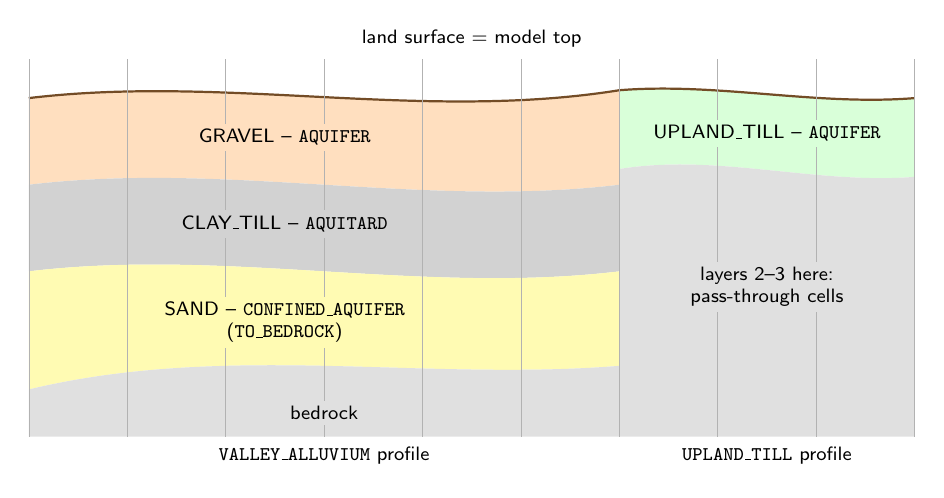
\begin{tikzpicture}[x=1.25cm,y=1.0cm,lab/.style={font=\scriptsize,align=center,inner sep=2pt}]
\fill[orange!25] (0,4.3) .. controls (2,4.6) and (4,4.0) .. (6,4.4) -- (6,3.2) .. controls (4,2.9) and (2,3.5) .. (0,3.2) -- cycle;
\fill[gray!35] (0,3.2) .. controls (2,3.5) and (4,2.9) .. (6,3.2) -- (6,2.1) .. controls (4,1.8) and (2,2.4) .. (0,2.1) -- cycle;
\fill[yellow!30] (0,2.1) .. controls (2,2.4) and (4,1.8) .. (6,2.1) -- (6,0.9) .. controls (4,0.7) and (2,1.2) .. (0,0.6) -- cycle;
\fill[black!12] (0,0.6) .. controls (2,1.2) and (4,0.7) .. (6,0.9) -- (6,0) -- (0,0) -- cycle;
\fill[green!15] (6,4.4) .. controls (7,4.5) and (8,4.2) .. (9,4.3) -- (9,3.3) .. controls (8,3.2) and (7,3.6) .. (6,3.4) -- cycle;
\fill[black!12] (6,0) -- (6,3.4) .. controls (7,3.6) and (8,3.2) .. (9,3.3) -- (9,0) -- cycle;
\draw[thick,brown!60!black] (0,4.3) .. controls (2,4.6) and (4,4.0) .. (6,4.4) .. controls (7,4.5) and (8,4.2) .. (9,4.3);
\foreach \x in {0,1,...,9} \draw[gray!60,very thin] (\x,0) -- (\x,4.8);
\node[lab,fill=white,inner sep=1pt] at (4.5,5.05) {land surface = model top};
\node[lab,fill=orange!25] at (2.6,3.8) {GRAVEL -- \cmd{AQUIFER}};
\node[lab,fill=gray!35] at (2.6,2.7) {CLAY\_TILL -- \cmd{AQUITARD}};
\node[lab,fill=yellow!30] at (2.6,1.45) {SAND -- \cmd{CONFINED\_AQUIFER}\\ (\cmd{TO\_BEDROCK})};
\node[lab,fill=black!12] at (3.0,0.3) {bedrock};
\node[lab,fill=green!15] at (7.5,3.85) {UPLAND\_TILL -- \cmd{AQUIFER}};
\node[lab,fill=black!12] at (7.5,1.9) {layers 2--3 here:\\ pass-through cells};
\node[lab,anchor=north] at (3,-0.05) {\cmd{VALLEY\_ALLUVIUM} profile};
\node[lab,anchor=north] at (7.5,-0.05) {\cmd{UPLAND\_TILL} profile};
\end{tikzpicture}
\caption{Layers are stacked from the model top and clipped at bedrock; the one-layer upland profile is padded with
pass-through cells.}\label{fig:layers}
\end{figure}

\subsection{Layer types}
\begin{table}[!htbp]\centering
\caption{Layer types.}\label{tab:types}\small
\begin{tabular}{P{0.31\linewidth}P{0.27\linewidth}P{0.348\linewidth}}\toprule\hdr
Type in the profile & MODFLOW 6 setting & What it means\\\midrule
\cmd{AQUIFER} (\cmd{UNCONFINED\_AQUIFER}) & \cmd{ICELLTYPE}=1, \cmd{ICONVERT}=1 & water table can be inside the layer: storage by $S_y$, transmissivity from the saturated thickness\\
\cmd{CONFINED\_AQUIFER} & \cmd{ICELLTYPE}=0, \cmd{ICONVERT}=0 & always full: constant transmissivity, storage by $S_s$\\
\cmd{AQUITARD} & as \cmd{AQUIFER}, with the low $K$ of its class & slow leaky layer, simulated explicitly\\
\cmd{AQUICLUDE} & \cmd{IDOMAIN}=0 & no flow at all through this layer (not allowed as the top layer)\\\bottomrule
\end{tabular}
\end{table}

\subsection{Material properties}
Each layer takes its properties from its aquifer class (\cmd{:AquiferClasses}): horizontal conductivity $K_h$
(\cmd{K\_HORIZ}), vertical conductivity $K_v$ (\cmd{K\_VERT}, default $K_h/10$), $S_s$ (\cmd{SPEC\_STORAGE}, default
$10^{-5}$), $S_y$ (\cmd{SPEC\_YIELD}, default 0.1) and porosity (\cmd{POROSITY}, default 0.3; stored for future transport
calculations; MODFLOW's flow calculation does not use it).

\begin{watch}
By default (\cmd{:LayerConnection INDEX}) MODFLOW connects layer $\ell$ of one column sideways only to layer $\ell$ of its
neighbours. Where two profiles meet, list their layers in the same geological order, otherwise, for example, a gravel layer
may connect to a clay layer; or use \cmd{:LayerConnection ELEVATION} (Section~\ref{sec:layerconn}), which connects the
cells whose elevations overlap. (An existing model keeps its own connections.)
\end{watch}

\subsection{Initial heads}
The starting head of every cell in a column is
\begin{equation}
h^0_i=\max\!\left(z_{\mathrm{land},i}-d_0,\;z_{\mathrm{low},i}+0.1\right),
\end{equation}
where $d_0$ is the profile's \cmd{INITIAL\_HEAD\_DEPTH} (or the value given by \cmd{:InitialGWHeads} in the \cmd{.rvc}
file), and $z_{\mathrm{low},i}$ is the bottom of the lowest active cell. With \cmd{:InitialGWHeads ELEVATION z}, $z$ replaces $z_{\mathrm{land},i}-d_0$ (still at least 0.1 m above the lowest active cell bottom).
A hotstart (\cmd{:GWHeads} in the \cmd{.rvc}) overrides all of this cell by cell. Optionally, a steady-state
calculation replaces these first guesses (Section~\ref{sec:init}).
When $d_0$ is larger than the layers above the water table are thick, a whole layer can start dry. Raven checks this at
start-up (cold start without a steady-state period, or hotstart heads): a layer whose active convertible cells all start at
or below their bottom gets one warning naming the layer and a line ``dry at the start'' in \cmd{GWModelSummary.txt}.
MODFLOW then has to rewet the whole layer in the first steps, which can take many iterations or leave some of them
unconverged; start from \cmd{:GWInitialization STEADY\_STATE}, a smaller \cmd{INITIAL\_HEAD\_DEPTH} or
\cmd{:InitialGWHeads}. Confined layers (\cmd{CONFINED\_AQUIFER}) never dry and are not checked.

\subsection{The generated MODFLOW files}
Raven writes a standard MODFLOW~6 simulation to \cmd{<output>/mf6/}: \cmd{mfsim.nam} (simulation), \cmd{sim.tdis}
(time steps), \cmd{sim.ims} (solver), \cmd{gwf.nam} (model), \cmd{gwf.dis} (grid), \cmd{gwf.npf} (conductivities and
layer types), \cmd{gwf.sto} (storage), \cmd{gwf.ic} (initial heads), \cmd{gwf.oc} (output control) and one file per
exchange package (\cmd{gwf.rch}, \cmd{gwf.drn}, \cmd{gwf.riv}, \cmd{gwf.evt}, \cmd{gwf.wel}, \cmd{gwf.ghb}, \cmd{gwf.chd},
\cmd{gwf.swx}, \cmd{gwf.res}). Grid arrays are written layer by layer, each grid row starting on a new line, which is
how MODFLOW reads them. These files can be opened in FloPy or ModelMuse; they never need editing.

\section{Parameters for building the model}\label{sec:buildparams}
The grid and layers are built from the following parameters; the class column says where each is set, the reference column
where its default and allowed range are listed.
\begin{table}[!htbp]\centering
\caption{Parameters for building the model.}
\begin{tabular}{>{\raggedright\arraybackslash}P{0.09\linewidth}>{\raggedright\arraybackslash}P{0.26\linewidth}>{\raggedright\arraybackslash}P{0.287\linewidth}>{\raggedright\arraybackslash}P{0.1\linewidth}>{\raggedright\arraybackslash}P{0.15\linewidth}}\toprule\hdr
Symbol & Parameter & Class (where it is set) & Units & Reference\\\midrule
$\Delta$ & \cmd{:GridCellSize} & \cmd{.rvg} option & m & Sec.~\ref{app:commands}\\
$f_{\min}$ & \cmd{:MinCellCoverage} & \cmd{.rvg} option & -- & Sec.~\ref{app:commands}\\
-- & \cmd{AQUIFER\_PROFILE} & HRU attribute (\cmd{:HRUs}, \cmd{.rvh}) & -- & Sec.~\ref{app:commands}\\
$P_k$ & HRU polygon & \cmd{:HRUGeometry} (\cmd{.rvg}) & -- & Sec.~\ref{app:commands}\\
$z_{\mathrm{land}}$ & land surface & \cmd{:LandSurface} (\cmd{.rvg}); else HRU \cmd{ELEVATION} & m & Sec.~\ref{app:commands}\\
$z_{\mathrm{br}}$ & bedrock & \cmd{:BedrockSurface} (\cmd{.rvg}); else \cmd{DEFAULT\_BEDROCK\_DEPTH} (aquifer profile) & m & Sec.~\ref{app:profile}\\
$d_{\mathrm{sz},a}$ & \cmd{SOIL\_ZONE\_DEPTH} & aquifer profile $a$ & m & Sec.~\ref{app:profile}\\
$b_\ell$ & layer thickness, type & aquifer profile (\cmd{:AquiferProfiles}) & m & Sec.~\ref{app:layers}\\
$K_h$, $K_v$ & \cmd{K\_HORIZ}, \cmd{K\_VERT} & aquifer class of the layer & m/d & Sec.~\ref{app:class}\\
$S_s$, $S_y$ & \cmd{SPEC\_STORAGE}, \cmd{SPEC\_YIELD} & aquifer class of the layer & 1/m, -- & Sec.~\ref{app:class}\\
$d_0$ & \cmd{INITIAL\_HEAD\_DEPTH}; \cmd{:InitialGWHeads} & aquifer profile; \cmd{.rvc} & m & Sec.~\ref{app:profile}\\
\bottomrule
\end{tabular}
\end{table}

\section{What the generated files look like}
The model name file lists the packages Raven uses:
\begin{lstlisting}
BEGIN OPTIONS
  NEWTON
END OPTIONS
BEGIN PACKAGES
  DIS6  gwf.dis  DIS
  NPF6  gwf.npf  NPF
  STO6  gwf.sto  STO
  IC6   gwf.ic   IC
  RCH6  gwf.rch  RCH_RAVEN
  DRN6  gwf.drn  DRN_RAVEN
  RIV6  gwf.riv  RIV_RAVEN
  OC6   gwf.oc   OC
END PACKAGES
\end{lstlisting}
The grid file records the projection in its first line, so the grid can be placed on a map:
\par\noindent\begin{minipage}{\linewidth}
\begin{lstlisting}
# Lambert azimuthal equal-area projection, origin lat=58.81662353 lon=-125.4914706 (sphere R=6371007.181 m)
BEGIN DIMENSIONS
  NLAY 3
  NROW 85
  NCOL 54
END DIMENSIONS
\end{lstlisting}
\end{minipage}\par\smallskip
Boundary packages contain one line per cell with placeholder values; Raven replaces the values in memory every step, so
the files show the grid positions of recharge, drains, rivers, wells and boundaries but not their daily values.

\section{Solver settings}
Why such a small head tolerance? MODFLOW stops iterating when no head changes by more than the tolerance, but a flow is a
conductance times a head difference. The seepage drains have very large conductances (one 1 km cell with a leakance of
1~d$^{-1}$ has $10^6$~m$^2$/d), so a head tolerance of 1 cm could still leave about $10^4$~m$^3$/d of imbalance in such a cell on a
difficult day. With 0.01 mm the imbalance is a thousand times smaller than with 1 cm. The price is more Newton iterations --- in the
20-year Liard run about 10 per day on average instead of 7--8 --- and a run about twice as long. The value was chosen from the
randomized tests: at 0.1 mm a few extreme set-ups (drain conductance $2\times10^7$~m$^2$/d per cell) still showed a 0.2\%
residual on single steps; at 0.01 mm none did.

\paragraph{Two-tier convergence.} A very tight tolerance can occasionally stall the Newton iterations on a hard step. The target is the tolerance above. If a step has not reached it after 100 iterations (or half the iteration limit, if that is smaller), the coupler raises
MODFLOW's own tolerance to ten times the target (0.1 mm) for the rest of that step only, and restores it for the next step. MODFLOW's own test always decides whether a step has converged. A step accepted at the relaxed tolerance is therefore as
reliable as a step of a model run with that tolerance. Only if even that fails within the iteration limit is the step
reported as not converged. \cmd{GWBudget.csv} records which
case applied (\emph{converged} = 1 target reached, 2 accepted at the relaxed tolerance, 0 not converged).
The water exchanged between Raven and MODFLOW is exact at any tolerance --- both sides use the same computed flows ---
so the tolerance only controls MODFLOW's own small numerical residual.

\begin{table}[!htbp]\centering
\caption{MODFLOW solver settings (\cmd{sim.ims}).}
\begin{tabular}{P{0.36\linewidth}P{0.14\linewidth}P{0.428\linewidth}}\toprule\hdr
IMS setting & Value & Meaning\\\midrule
\cmd{COMPLEXITY} & \cmd{COMPLEX} & robust defaults for non-linear problems\\
\cmd{OUTER\_DVCLOSE} & 0.00001 m & Newton iterations stop when no head changes by more than this (\cmd{:SolverHead\allowbreak Tolerance})\\
\cmd{OUTER\_MAXIMUM} & 500 & iteration limit (\cmd{:SolverMax\allowbreak OuterIterations})\\
\cmd{UNDER\_RELAXATION} & \cmd{DBD} & damps oscillating head changes (theta 0.7, kappa 0.07, gamma 0.1)\\
\cmd{BACKTRACKING\_NUMBER} & 20 & retries with a smaller step when the imbalance grows\\
\cmd{INNER\_MAXIMUM} & 500 & linear-solver iteration limit\\
\cmd{INNER\_DVCLOSE}, \cmd{INNER\_RCLOSE} & $0.1\times$ outer, 1 m$^3$/d & linear-solver tolerances\\
\cmd{LINEAR\_ACCELERATION} & \cmd{BICGSTAB} & linear solver\\
\cmd{PRECONDITIONER\_LEVELS} & 5 & ILU fill level\\\bottomrule
\end{tabular}
\end{table}

\section{How MODFLOW solves each time step}\label{ch:mf6}
\subsection{Time steps}
MODFLOW's time steps are generated from Raven's \cmd{:StartDate}, \cmd{:Duration} ($t_{\mathrm{end}}$) and \cmd{:TimeStep} ($\dt$): one transient
stress period of $N=\mathrm{round}(t_{\mathrm{end}}/\dt)$ steps of length $\dt$, preceded by a one-day steady-state period when
\cmd{:GWInitialization STEADY\_STATE} is used. MODFLOW therefore always takes exactly one step for each Raven step.
If Raven would run more steps than MODFLOW holds, Raven stops with a clear message.

\subsection{Cells that dry and rewet: the Newton method}
An unconfined cell whose water table falls below its bottom is \emph{dry}. Older MODFLOW versions switched such cells
off, which often made the solution fail when they needed to switch back on. MODFLOW~6's Newton--Raphson method, which the coupling always uses, keeps dry cells in the calculation. The conductance
between two cells is scaled smoothly by how full the upstream cell is, and falls to zero as that cell empties. The cell
fills again naturally when water arrives. The solver settings written by Raven are:
\begin{itemize}
\item outer (Newton) iterations up to 500 (\cmd{:SolverMax\allowbreak OuterIterations}), head-change tolerance 0.00001 m (\cmd{:SolverHead\allowbreak Tolerance});
\item delta-bar-delta under-relaxation (damps oscillating head changes) and backtracking (retries a smaller change
when the residual grows);
\item inner linear solver BiCGSTAB with an ILU preconditioner of level 5, residual tolerance 1.0 m$^3$/d.
\end{itemize}
The Newton option is written without its own \cmd{UNDER\_RELAXATION} keyword, which resets a head that falls below the cell
bottom. With MODFLOW~6.6 that reset made the Newton change of a drying cell repeat unchanged at every iteration, so the
step never converged (on the Liard model this happened on most days once the thin aquitard under the gravel began to dry).
Without it, MODFLOW~6.6.3 and 6.8.1 converge in the same few iterations.
Raven runs the Newton iterations itself through MODFLOW's interface (prepare, repeated solve, finalize), so it knows
whether each step converged. If a step does not converge, MODFLOW continues (option \cmd{CONTINUE}), the step is
flagged in \cmd{GWBudget.csv}, and a safeguard limits what that step can return to Raven (Section~\ref{sec:guard}).

\subsection{Connectivity between aquifer areas}
Because dry cells carry no flow, parts of an aquifer can become disconnected when the water table falls and join
again when it rises, without any action by the user. Streams disconnect from a falling water table in the same way
(Section~\ref{ch:rivers}). To show this, \cmd{GWConnectivity.csv} reports each step:
\begin{itemize}
\item the fraction of top-layer cells of each profile that are \emph{wet}, meaning $h_i>z^{(1)}_{\mathrm{bot},i}+10^{-3}$ m;
\item the number of separate wet areas, where two wet cells belong to the same area if they share an edge
(4-neighbour connectivity; counted by a flood-fill of the wet cells).
\end{itemize}
This is a diagnostic only; it does not affect the calculation.

\subsection{Heads of dry cells}
Under the Newton method a dry cell carries no flow, and MODFLOW leaves its head at whatever value the solver reaches; it
can be far below the cell bottom (values of $-10^{8}$~m have been seen in a pumped, isolated cell). MODFLOW's own flows are
unaffected, but such a head is not a water level. Wherever the coupling needs a real water level it therefore uses the \emph{water table} of the column: the head of the
highest cell whose head is above its bottom, or the bottom of the lowest active cell if all are dry. This is used for the
reservoir's local groundwater level, in \cmd{GWHRUState.csv}, and for monitoring wells (a well screened in a dry cell
reports a missing value, \cmd{-1.2345}). The MODFLOW head file and the hotstart heads keep
MODFLOW's raw values, so a restart continues exactly.

\chapter{Coupling an existing MODFLOW 6 model}\label{ch:existing}

\begin{plain}
You give Raven your MODFLOW~6 model and tell it three things: where the model lies on the map, on what calendar date the
model's time starts, and which of the model's packages Raven should replace --- usually recharge and evaporation, which Raven
then supplies. Raven copies the model, makes the few changes shown in Figure~\ref{fig:workcopy}, and runs the copy together
with the Raven model, one day at a time. Your own files are never changed.
\end{plain}

Many users already have a calibrated MODFLOW~6 model and want to connect it to a Raven model. In this mode Raven does not
build a groundwater model. It takes the user's model as it is: the grid, the layers, the conductivities, storage, wells,
boundaries, stress periods and solver settings. Raven links its HRUs to the model's top active layer --- the highest layer
that holds water at each location --- and exchanges water there.

Only three things change, and only in a copy of the model (Figure~\ref{fig:workcopy}):
\begin{enumerate}
\item the stress periods are split into Raven time steps;
\item the packages that Raven takes over (usually recharge and evapotranspiration) are switched off;
\item Raven's packages are added: \cmd{RCH\_RAVEN} (recharge from Raven) and \cmd{DRN\_RAVEN} (seepage back to Raven), and, when
the \cmd{.rvp} and \cmd{.rvg} files ask for them, \cmd{EVT\_RAVEN} (water-table evaporation), \cmd{SWX\_RAVEN} (wetlands and lakes in
Raven stores) and \cmd{RES\_RAVEN} (reservoir seepage).
\end{enumerate}

\begin{figure}[!htbp]\centering% The working copy of an existing model (TikZ)
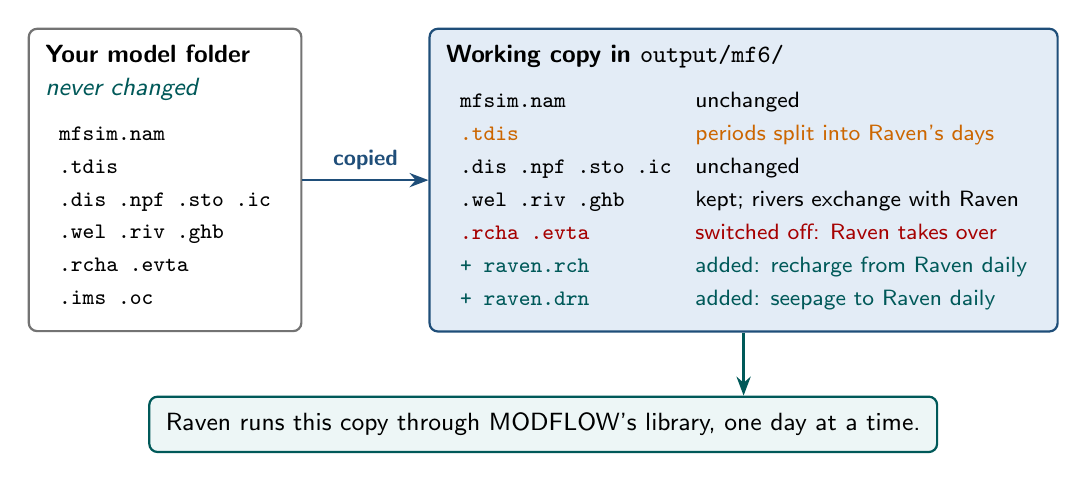
\begin{tikzpicture}[every node/.append style={execute at begin node={\hyphenpenalty=10000\exhyphenpenalty=10000}},font=\sffamily\small,arr/.style={-{Stealth[length=2.4mm]},line width=0.9pt}]
\node[draw=black!55,rounded corners=3pt,line width=0.8pt,fill=white,inner sep=6pt,align=left,anchor=north west] (L) at (0,0) {%
  \textbf{Your model folder}\\[1pt]{\itshape\color{teal!70!black}never changed}\\[5pt]
  {\footnotesize\ttfamily\begin{tabular}{l}mfsim.nam\\.tdis\\.dis .npf .sto .ic\\.wel .riv .ghb\\.rcha .evta\\.ims .oc\end{tabular}}};
\node[draw=brand,rounded corners=3pt,line width=0.8pt,fill=brandlight,inner sep=6pt,align=left,anchor=north west] (R) at ([xshift=16mm]L.north east) {%
  \textbf{Working copy in \texttt{output/mf6/}}\\[5pt]
  {\footnotesize\begin{tabular}{l@{\hspace{3mm}}l}
  \texttt{mfsim.nam} & unchanged\\
  \textcolor{orange!80!black}{\texttt{.tdis}} & \textcolor{orange!80!black}{periods split into Raven's days}\\
  \texttt{.dis .npf .sto .ic} & unchanged\\
  \texttt{.wel .riv .ghb} & kept; rivers exchange with Raven\\
  \textcolor{red!65!black}{\texttt{.rcha .evta}} & \textcolor{red!65!black}{switched off: Raven takes over}\\
  \textcolor{teal!70!black}{\texttt{+ raven.rch}} & \textcolor{teal!70!black}{added: recharge from Raven daily}\\
  \textcolor{teal!70!black}{\texttt{+ raven.drn}} & \textcolor{teal!70!black}{added: seepage to Raven daily}\\
  \end{tabular}}};
\draw[arr,brand] (L.east |- R.center) -- node[above,font=\sffamily\bfseries\footnotesize,text=brand]{copied} (R.west |- R.center);
\node[draw=teal!70!black,rounded corners=3pt,line width=0.8pt,fill=teal!7,inner sep=6pt,anchor=north] (B) at ([yshift=-8mm]current bounding box.south) {Raven runs this copy through MODFLOW's library, one day at a time.};
\draw[arr,teal!70!black] (R.south) -- (R.south |- B.north);
\end{tikzpicture}

\caption{Raven runs a working copy of the model. The copy differs from the original in three ways only; the original folder is never changed.}\label{fig:workcopy}
\end{figure}

The approach follows L.~Scantlebury's MODFLOW-USG coupling, which linked the top layer of an existing model to HRUs
through a table of overlap weights. It works for any grid, because only the top layer is linked and the model's cells are
found through MODFLOW's own memory. Regular (DIS) and polygon (DISV) grids are supported.

\section{A complete example}
\begin{lstlisting}
# Liard.rvg - Raven coupled to an existing MODFLOW 6 model
:HRUGeometry      Liard_HRUs.geojson  HRU_ID       # HRU polygons (lon/lat)
:MF6Library       /opt/mf6/libmf6.so
:MF6Simulation    model/mfsim.nam                  # the existing simulation
:MF6CRS           EPSG:32610                       # projection of the model's coordinates
:MF6StartDate     1985-10-01                       # date of the model's time zero
:RavenTakesOver   RCH_MODEL EVT_MODEL              # packages Raven replaces
:StreamPackage    RIV_STREAMS AUX SUBBASIN         # river cells linked to Raven's reaches
:SeepageToRaven   ON                               # groundwater seeping out returns to Raven
\end{lstlisting}
HRUs with an \cmd{AQUIFER\_PROFILE} in the \cmd{.rvh} file are coupled, as in the generated mode. The layer geometry and
hydraulic properties come from the model's own files, so a profile needs no layers and no \cmd{:AquiferClasses} are
needed: give it as \cmd{name, 0} in \cmd{:AquiferProfiles}. The profile then only marks the coupled HRUs and carries the
exchange settings in \cmd{:AquiferProfileParameters} (\cmd{SEEPAGE\_LEAKANCE}, \cmd{SEEPAGE\_SMOOTHING\_DEPTH},
\cmd{RECHARGE\_DELAY}, \cmd{EXTINCTION\_DEPTH}); its other parameters are not used. Layers listed in a profile are ignored, with a warning.
\begin{lstlisting}
:AquiferProfiles
  VALLEY_ALLUVIUM, 0                 # no layers: the model's own are used
  UPLAND_TILL,     0
:EndAquiferProfiles
:AquiferProfileParameters
  :Attributes,     SEEPAGE_LEAKANCE
  :Units,          1/d
  VALLEY_ALLUVIUM, 1.0
  UPLAND_TILL,     1.0
:EndAquiferProfileParameters
\end{lstlisting}
Raven's recharge must reach the \cmd{GROUNDWATER} store, exactly as in Section~\ref{sec:buildparams}.

\section{Linking HRUs to the model's cells}
Raven needs to know which grid cells lie under each HRU. MODFLOW model files do not say where on Earth the model is, so the
user supplies that information in one of three ways (give exactly one). Each coupled HRU is then linked to the top active
cell of every column it overlaps.

\paragraph{\cmd{:MF6CRS} (recommended).}\label{sec:mf6crs} The user names the model's map projection, usually as a standard EPSG code. Raven
reads the cell outlines from the model itself (column and row widths, origin and rotation for DIS grids; the cell corners for
DISV grids) and places them on the map with that projection (Figure~\ref{fig:placing}).
\begin{figure}[!htbp]\centering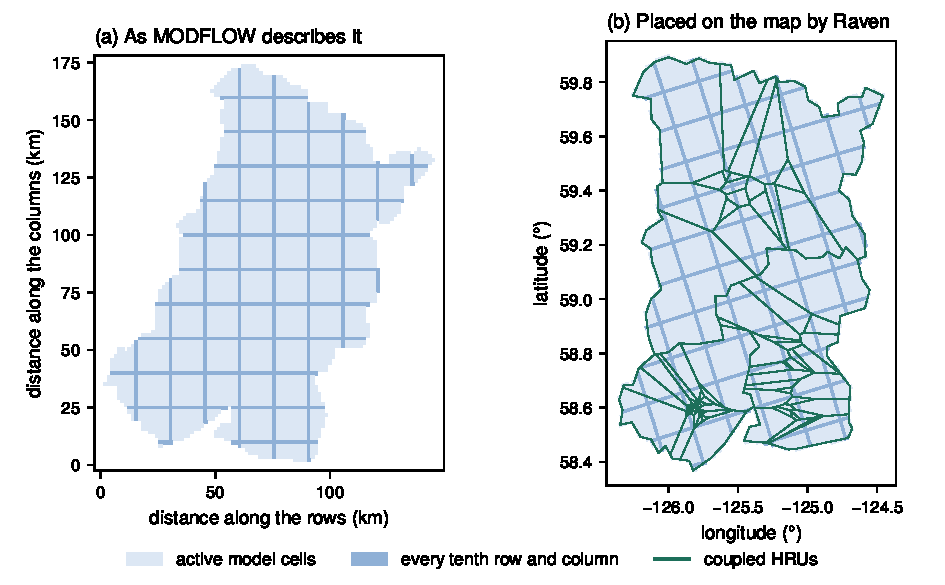
\includegraphics[width=0.95\linewidth]{figures/fig_placing.pdf}
\caption{The synthetic Liard model's cells: (a) as MODFLOW describes them, in the model's own rotated coordinates; (b) placed on the map by Raven from the projection \cmd{EPSG:32610}, under the Raven HRUs.}\label{fig:placing}
\end{figure}
 Built-in projections need no external software: Transverse Mercator (every UTM zone, north and south), Albers
equal-area and Lambert conformal conic, on the WGS84 or GRS80 (NAD83) ellipsoid. Common codes are recognised directly:
\begin{center}\small
\begin{tabularx}{\linewidth}{P{0.46\linewidth}Y}\toprule\hdr
Code & Projection\\\midrule
\cmd{EPSG:32601}--\cmd{32660}, \cmd{EPSG:32701}--\cmd{32760} & WGS84 / UTM zones, north and south\\
\cmd{EPSG:26901}--\cmd{26923} & NAD83 / UTM zones 1--23 north\\
\cmd{EPSG:3005} & NAD83 / BC Albers\\
\cmd{ESRI:102001} (or \cmd{EPSG:102001}) & Canada Albers equal-area conic (an ESRI code)\\
\cmd{EPSG:5070} & NAD83 / CONUS Albers\\
\cmd{EPSG:3978}, \cmd{EPSG:3347} & NAD83 / Canada Atlas Lambert; Statistics Canada Lambert\\\bottomrule
\end{tabularx}\end{center}
Any other projection of these three kinds is given by its parameters:
\begin{lstlisting}
:MF6CRS TMERC  lat0 lon0 k0 FE FN {WGS84|GRS80}
:MF6CRS ALBERS lat1 lat2 lat0 lon0 FE FN {WGS84|GRS80}
:MF6CRS LCC    lat1 lat2 lat0 lon0 FE FN {WGS84|GRS80}
\end{lstlisting}
The parameters are read as for \cmd{:InputCRS} (Section~\ref{sec:inputcrs}); conic parameters that define no cone
(standard parallels symmetric about the equator, an \cmd{LCC} parallel at a pole) stop the run. The built-in formulas
(Karney's series for Transverse Mercator, Snyder's for the conics) agree with the PROJ library to a few
micrometres (Section~\ref{sec:vexisting}). The small datum difference between NAD83 and WGS84 (about a metre) is ignored.

\paragraph{\cmd{:MF6GridFile}.} A GeoJSON file of the top-layer cells in longitude/latitude (or in the projection of
\cmd{:InputCRS}, Section~\ref{sec:inputcrs}, which also applies to \cmd{:HRUGeometry} and \cmd{:LandSurface}), numbered by an ID field
(default \cmd{CELL\_ID}) from 1 to the number of cells in a layer, as exported by GIS software. Raven checks that there is one
polygon per cell and that the polygons are the model's cells in the model's order. A map projection scales areas and turns
directions slightly, so Raven allows one common scale and one common rotation, and nothing else:
\begin{itemize}
\item every polygon's area, divided by the area MODFLOW gives the cell, must be the same for all cells within 5\%, and this
      common ratio must lie between 0.8 and 1.25 (a wrong length unit gives about 0.09 or 10.8);
\item for every pair of neighbouring cells MODFLOW connects, the two polygons must lie as far apart and in the same direction
      as MODFLOW's cells, within 20\% and 15\textdegree{} after the common scale and rotation. A shuffled numbering changes
      the distances; a mirrored one (for example rows numbered from the south: MODFLOW's row 1 is the northern row) turns
      directions around.
\end{itemize}
A file that fails either check stops the run with a message naming the first cell that does not fit.
\cmd{GWModelSummary.txt} reports the common area ratio.

\paragraph{\cmd{:OverlapWeights}.} The table of the MODFLOW-USG coupling, prepared outside Raven:
\begin{lstlisting}
:OverlapWeights
  # [HRU ID] [cell] [w = overlap area / cell area]
  2736   1204   0.35
  2736   1205   1.0
:EndOverlapWeights
\end{lstlisting}
No HRU polygons are needed. Monitoring wells cannot be located with this option.

\paragraph{No water is lost on the way.} Each HRU's recharge is shared among the cells it covers, in proportion to how much of
the HRU lies in each cell (Figure~\ref{fig:linking}a). The shares always add up to 100\%, so all the water Raven sends
arrives in MODFLOW --- even when the HRU polygons or the weights do not quite match the HRU areas in the \cmd{.rvh} file. A
mismatch changes only \emph{where} inside the HRU the water lands, not \emph{how much} (Figure~\ref{fig:linking}b). In
formula form, cell $i$ receives $V_{k\to i}=\frac{r_k}{1000}\,10^{6}A_k\,A_{k,i}/\sum_j A_{k,j}$ from HRU $k$ (Section~\ref{sec:linkage}).

\begin{figure}[!htbp]\centering% HRU over grid cells with its share in each cell (generated by make_tikz_linking.py; shares computed from the shapes)
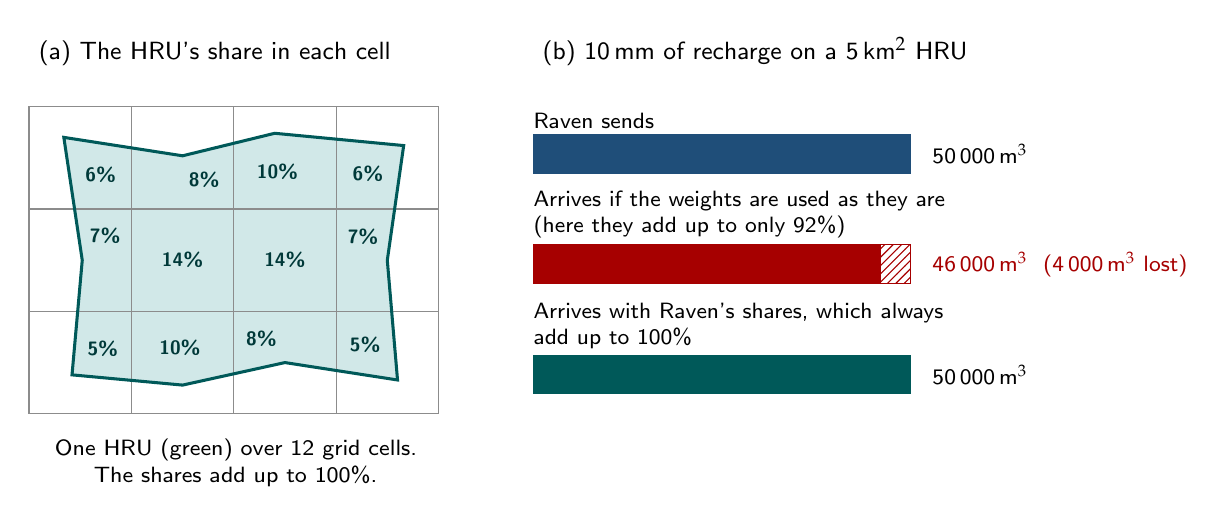
\begin{tikzpicture}[x=1mm,y=1mm,font=\sffamily\footnotesize,every node/.append style={execute at begin node={\hyphenpenalty=10000\exhyphenpenalty=10000}}]
\node[anchor=south west,font=\sffamily\small] at (0,43) {(a) The HRU's share in each cell};
\fill[teal!18] (5.46,4.94) -- (19.50,3.64) -- (32.50,6.50) -- (46.80,4.29) -- (45.50,19.50) -- (47.58,34.06) -- (31.20,35.62) -- (19.50,32.76) -- (4.42,35.10) -- (6.76,19.50) -- cycle;
\draw[black!45,line width=0.4pt] (0,0) rectangle (13,13);
\draw[black!45,line width=0.4pt] (0,13) rectangle (13,26);
\draw[black!45,line width=0.4pt] (0,26) rectangle (13,39);
\draw[black!45,line width=0.4pt] (13,0) rectangle (26,13);
\draw[black!45,line width=0.4pt] (13,13) rectangle (26,26);
\draw[black!45,line width=0.4pt] (13,26) rectangle (26,39);
\draw[black!45,line width=0.4pt] (26,0) rectangle (39,13);
\draw[black!45,line width=0.4pt] (26,13) rectangle (39,26);
\draw[black!45,line width=0.4pt] (26,26) rectangle (39,39);
\draw[black!45,line width=0.4pt] (39,0) rectangle (52,13);
\draw[black!45,line width=0.4pt] (39,13) rectangle (52,26);
\draw[black!45,line width=0.4pt] (39,26) rectangle (52,39);
\draw[teal!70!black,line width=1.1pt] (5.46,4.94) -- (19.50,3.64) -- (32.50,6.50) -- (46.80,4.29) -- (45.50,19.50) -- (47.58,34.06) -- (31.20,35.62) -- (19.50,32.76) -- (4.42,35.10) -- (6.76,19.50) -- cycle;
\node[font=\sffamily\bfseries\scriptsize,text=teal!45!black,inner sep=0.5pt] at (9.37,8.21) {5\%};
\node[font=\sffamily\bfseries\scriptsize,text=teal!45!black,inner sep=0.5pt] at (9.67,22.57) {7\%};
\node[font=\sffamily\bfseries\scriptsize,text=teal!45!black,inner sep=0.5pt] at (9.10,30.37) {6\%};
\node[font=\sffamily\bfseries\scriptsize,text=teal!45!black,inner sep=0.5pt] at (19.17,8.35) {10\%};
\node[font=\sffamily\bfseries\scriptsize,text=teal!45!black,inner sep=0.5pt] at (19.50,19.50) {14\%};
\node[font=\sffamily\bfseries\scriptsize,text=teal!45!black,inner sep=0.5pt] at (22.24,29.67) {8\%};
\node[font=\sffamily\bfseries\scriptsize,text=teal!45!black,inner sep=0.5pt] at (29.53,9.47) {8\%};
\node[font=\sffamily\bfseries\scriptsize,text=teal!45!black,inner sep=0.5pt] at (32.50,19.50) {14\%};
\node[font=\sffamily\bfseries\scriptsize,text=teal!45!black,inner sep=0.5pt] at (31.56,30.78) {10\%};
\node[font=\sffamily\bfseries\scriptsize,text=teal!45!black,inner sep=0.5pt] at (42.70,8.71) {5\%};
\node[font=\sffamily\bfseries\scriptsize,text=teal!45!black,inner sep=0.5pt] at (42.43,22.47) {7\%};
\node[font=\sffamily\bfseries\scriptsize,text=teal!45!black,inner sep=0.5pt] at (43.05,30.47) {6\%};
\node[anchor=north,align=center,text width=50mm] at (26,-2) {One HRU (green) over 12 grid cells.\\The shares add up to 100\%.};
\node[anchor=south west,font=\sffamily\small] at (64,43) {(b) 10\,mm of recharge on a 5\,km$^2$ HRU};
\node[anchor=south west,align=left,inner sep=0pt] at (64,36.2) {Raven sends};
\fill[brand] (64,30.5) rectangle (112,35.5);
\node[anchor=west] at (113.5,33) {50\,000\,m$^3$};
\node[anchor=south west,align=left,inner sep=0pt] at (64,22.2) {Arrives if the weights are used as they are\\(here they add up to only 92\%)};
\fill[red!65!black] (64,16.5) rectangle (108.16,21.5);
\draw[red!65!black,pattern=north east lines,pattern color=red!65!black] (108.16,16.5) rectangle (112,21.5);
\node[anchor=west,text=red!65!black] at (113.5,19) {46\,000\,m$^3$ \ (4\,000\,m$^3$ lost)};
\node[anchor=south west,align=left,inner sep=0pt] at (64,8.2) {Arrives with Raven's shares, which always\\add up to 100\%};
\fill[teal!70!black] (64,2.5) rectangle (112,7.5);
\node[anchor=west] at (113.5,5) {50\,000\,m$^3$};
\end{tikzpicture}

\caption{Sharing an HRU's water among cells. (a) The HRU's share in each cell, computed from the shapes; the shares add up to 100\%. (b) Weights that add up to only 92\% would lose 8\% of the water; Raven's shares always add up to 100\%, so every cubic metre arrives.}\label{fig:linking}
\end{figure}

Using the weights as given would make the recharge volume depend on how carefully the HRUs were drawn. Rates passed to MODFLOW use MODFLOW's own cell areas. \cmd{GWModelSummary.txt} reports how much of the coupled
HRUs' area lies on active cells; a low value usually means a wrong projection or HRUs outside the model.

\section{Time}\label{sec:existingtime}
MODFLOW models divide time into \emph{stress periods}: stretches of time, often a month, during which inputs such as pumping
rates stay the same. Raven works in days. Raven keeps the model's stress periods and their dates, and splits each period into
Raven days (Figure~\ref{fig:periods}), so the model's own changes --- a well pumping harder in summer, a boundary level
changing --- still happen on their dates.

\cmd{:MF6StartDate} is the calendar date on which the model's time starts, with its time of day when that is not midnight
(\cmd{1985-10-01 12:00:00} or \cmd{1985-10-01T12:00:00}); any other text after the date stops the run. Each stress period must contain a whole number of
Raven time steps, and Raven's run may not go past the end of the model; otherwise the run stops with a message. Steady-state
periods (solved as the long-term balance) stay steady-state.

\paragraph{Steady-state models.} Many calibrated models are steady state: no storage package (or one that marks every period
steady) and a single stress period whose length has no meaning (often one second or one day). Raven stretches that period
over its run, so every Raven step is a steady-state solution with that step's recharge: the aquifer responds at once, without
storage. \cmd{GWModelSummary.txt} says so, and the storage column of \cmd{GWBudget.csv} stays zero (the balance residual is
reported as MODFLOW's error). Because such a model has no time of its own, Raven may start on any date from
\cmd{:MF6StartDate} on.

\begin{figure}[!htbp]\centering% Stress periods, Raven's days and a restart after 40 days (TikZ; 1 mm per day)
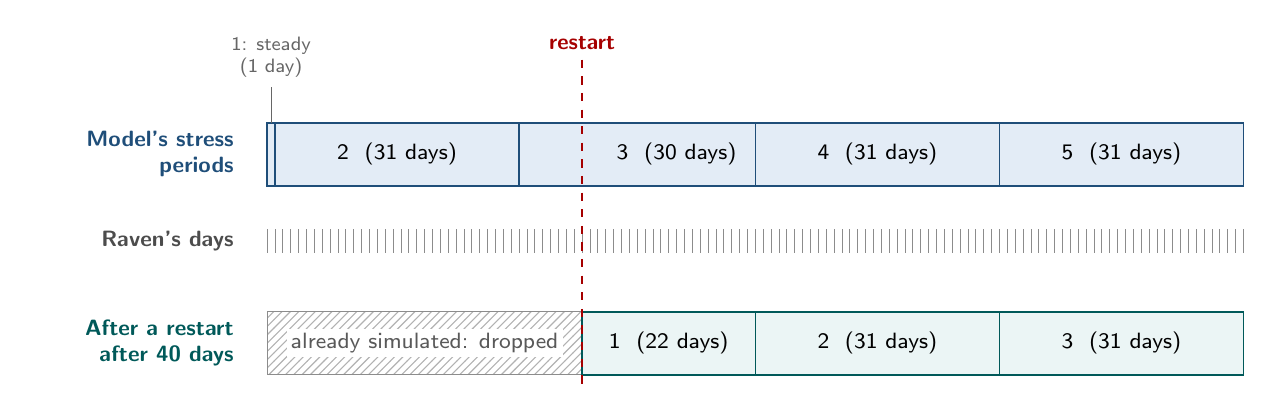
\begin{tikzpicture}[every node/.append style={execute at begin node={\hyphenpenalty=10000\exhyphenpenalty=10000}},x=1mm,y=1mm,font=\sffamily\footnotesize,
  rowlab/.style={anchor=east,align=right,text width=25mm,font=\sffamily\footnotesize\bfseries},
  per/.style={draw=brand,fill=brandlight,line width=0.6pt},
  new/.style={draw=teal!70!black,fill=teal!8,line width=0.6pt}]
% row 1: the model's stress periods (1 steady day, then 31, 30, 31, 31 days)
\node[rowlab,text=brand] at (-3,0) {Model's stress\\periods};
\draw[per] (0,-4) rectangle (1,4);
\foreach \a/\b/\t/\lx in {1/32/{2 \ (31 days)}/16.5, 32/62/{3 \ (30 days)}/52, 62/93/{4 \ (31 days)}/77.5, 93/124/{5 \ (31 days)}/108.5}{
  \draw[per] (\a,-4) rectangle (\b,4); \node at (\lx,0) {\t};}
\draw[black!60] (0.5,4) -- (0.5,8.5) node[above,align=center,font=\sffamily\scriptsize] {1: steady\\(1 day)};
% row 2: Raven's days
\node[rowlab,text=black!70] at (-3,-11) {Raven's days};
\foreach \d in {0,...,124}{\draw[black!45,line width=0.3pt] (\d,-12.5) -- (\d,-9.5);}
% row 3: after a restart after 40 days
\node[rowlab,text=teal!70!black] at (-3,-24) {After a restart\\after 40 days};
\draw[black!45,fill=black!6,pattern=north east lines,pattern color=black!30] (0,-28) rectangle (40,-20);
\node[fill=white,inner sep=1.5pt,text=black!65] at (20,-24) {already simulated: dropped};
\foreach \a/\b/\t in {40/62/{1 \ (22 days)}, 62/93/{2 \ (31 days)}, 93/124/{3 \ (31 days)}}{
  \draw[new] (\a,-28) rectangle (\b,-20); \node at ({(\a+\b)/2},-24) {\t};}
% the restart
\draw[red!65!black,dashed,line width=0.9pt] (40,12) -- (40,-30);
\node[above,text=red!65!black,font=\sffamily\bfseries\footnotesize] at (40,12) {restart};
\end{tikzpicture}

\caption{Top: a model with a one-day steady period followed by periods of 31, 30, 31 and 31 days, and Raven's days. Bottom: after a restart 40 days into the model, the time already simulated is dropped, period~3 keeps its last 22 days, and the periods are renumbered; each keeps its own well rates and boundary levels.}\label{fig:periods}
\end{figure}

\paragraph{Starting later: restarts.} Raven may start later than the model's time zero --- when a run is continued from
\cmd{solution.rvc}, or begins part-way through the model. Raven then removes the stress periods already simulated from the
working copy, shortens the period that holds Raven's start, and renumbers the periods of every package; the new first period
takes the inputs that were in force on Raven's start date (Figure~\ref{fig:periods}, bottom). This is safe for packages whose period
entries replace one another (WEL, RIV, GHB, CHD, DRN, list-based RCH and EVT, STO, OC, the water mover MVR, the flow barriers HFB,
and the stress offsets of CSUB), and for array-based recharge and ET, packages read as arrays (\cmd{READASARRAYS}, \cmd{READARRAYGRID}:
an array a period entry leaves out keeps its earlier values) and the advanced packages (SFR, LAK, MAW, UZF) when at most one period entry comes before Raven's
start. Such a package with several earlier entries, whose settings build on one another, stops such a run, as does
time-varying conductivity or storage (\cmd{TVK6}, \cmd{TVS6}); Raven must then start at \cmd{:MF6StartDate}. (A
simulation holding more than one model, or exchanges, stops at any start: Raven couples one model.) The times of a time series (\cmd{TS6} files) count from the
model's own time zero: on a later start, even one inside the first period, Raven shifts every time of each \cmd{TS6} file
named by a package it keeps by the time elapsed before its start. Entries before the start keep negative times,
so MODFLOW interpolates across Raven's start exactly as it did on the model's own clock. Time-array series (\cmd{TAS6}) stop
a later start; the rows of a \cmd{TS6} file read through
\cmd{OPEN/CLOSE} are shifted and written into the working copy's \cmd{TS6} file. A time of day in Raven's \cmd{:StartDate}
counts in the offset, so restarts work with sub-daily time steps too (the start must fall on a Raven step of its stress
period); the working copy's \cmd{START\_DATE\_TIME} is set to Raven's start, with the time of day when there is one.
Raven writes the rewritten periods, and the TDIS options, into the working copy's TDIS file. Raven reads the model's text files as
MODFLOW~6 reads them: a line whose first character other than a blank, comma or tab is \cmd{\#} or \cmd{!}, or that
begins with \cmd{//}, is a comment; blanks, commas and tabs separate the words, and a quoted word may hold them. Where
MODFLOW reads a fixed number of words (a period row, a time-series row), text after them is ignored; where it reads
every word of a line, such text is data, as for MODFLOW: an \cmd{AUXILIARY} line names one auxiliary variable per word,
and the third word of a name-file \cmd{PACKAGES} row names the package. A row without a third word is named as MODFLOW
names it: by its type and its place among all rows of that type, named or not (in \cmd{WEL6 a.wel WELA} followed by
\cmd{WEL6 b.wel}, the second is \cmd{WEL-2}); a type a model holds only once (\cmd{DIS}, \cmd{NPF}, \cmd{STO}, \cmd{IC},
\cmd{OC}, \ldots) is named by its type. These are the names MODFLOW's list file shows, and the names
\cmd{:RavenTakesOver}, \cmd{:KeepPackages} and \cmd{:StreamPackage} take. Raven writes each such name into its row of
the working copy, so that removing the rows it takes over does not change the names of the rest, and stops when MODFLOW
has no package of a name it reads, or reads a package of such a type that Raven did not find in the name file. As for
MODFLOW, the lines of an \cmd{OPEN/CLOSE} file in a block (any block but \cmd{GRIDDATA}; path relative to the simulation
folder, or absolute) are read in place of the \cmd{OPEN/CLOSE} line, which must be the block's first line other than
comments (elsewhere the run stops, as MODFLOW~6 refuses it). Every file Raven reads is read so: \cmd{mfsim.nam} and the
model name file, the TDIS file (its options, such as \cmd{TIME\_UNITS}, \cmd{START\_DATE\_TIME} and \cmd{ATS6}, and its
period data), the water mover (its \cmd{PACKAGES} and \cmd{PERIOD} blocks), the options of every package kept (\cmd{TS6},
\cmd{TAS6}, \cmd{TVK6}, \cmd{TVS6}, \cmd{READASARRAYS}, \cmd{AUXILIARY}), the \cmd{PERIOD} blocks of the storage package and
\cmd{TS6} files. An \cmd{OPEN/CLOSE} file marked binary stops the run there (Raven reads text). MODFLOW resolves the
paths a model's files name from the simulation folder, and Raven's working copy resolves them in the same way: in every file
MODFLOW reads (the simulation file, the TDIS and model name files, the packages kept, and the solution files and the files
named with \cmd{FILEIN}, such as \cmd{TS6} and \cmd{OBS6} files, in turn), an \cmd{OPEN/CLOSE} file outside the folder (a
\cmd{../} path) is named by its absolute path and read in place; a text \cmd{FILEIN} file (\cmd{TS6}, \cmd{TAS6}, \cmd{OBS6},
\cmd{TVK6}, \cmd{TVS6}, \cmd{ATS6}, \cmd{HPC6}, \cmd{MVR6}, \cmd{GNC6} and the like) or solution file outside the folder is
copied into the working copy, so that the paths it names are handled too and a time series can be shifted, while another
\cmd{FILEIN} file (\cmd{NETCDF}) is only named by its absolute path, never read or copied; an \cmd{OPEN/CLOSE} file of any
block but \cmd{GRIDDATA} is searched as the block's own lines, and when it names such a path, a copy of it in the working copy
is rewritten and read in its place (the user's file is left as it is); and an output
file (\cmd{FILEOUT}, the name file's \cmd{LIST}) named by an absolute path or a \cmd{../} path is written in the working
copy instead --- at its place in the folder when it lies there, else as \cmd{raven\_out\_}\emph{n}\cmd{\_}\emph{name} --- so
the run writes nothing outside Raven's output folder and never overwrites the user's files. \cmd{GWModelSummary.txt} names
each output file so placed and counts the files copied or read in place. A path that holds both a single and a double
quote cannot be written in a MODFLOW input line and stops the run. Where Raven writes a
working copy of a file (the name file, the TDIS file, the water mover, a \cmd{TS6} file), the rows of such a file are
written in place of the line, which is kept as a comment, so the rules of this section apply to them. As a second
guard, the time unit Raven read is compared with the one MODFLOW holds after it initialises the model, and a difference
(or adaptive time stepping) stops the run. A step that MODFLOW solves (converged) with a balance error above 1~\% of the gross flow gives a warning
once a run (a package outside Raven's books, or solver tolerances too loose). Period lengths, time-series times and period
numbers are read as MODFLOW reads them (Fortran list-directed input): \cmd{5}, \cmd{5.0E-1}, \cmd{50.0D-1} (\cmd{D},
\cmd{d}, \cmd{Q} or \cmd{E} for the exponent, which may be left without digits), \cmd{5.0/} (a slash ends the value),
\cmd{2*5.0} (a repeat count) and, for a period number, the whole part of such a value. A value that is not a number, or a
\cmd{PERIODDATA} block with other than \cmd{NPER} rows, stops the run, naming the file and the line.

\section{Units}
Length units (metres, feet, centimetres) are read from the discretization package and time units (seconds to years) from
the time discretization. Heads, flows, rates, conductances and coordinates are converted at the interface; Raven's outputs
are always in metres and days.

\section{Packages}
\begin{longtable}{P{0.24\linewidth}P{0.70\linewidth}}
\caption{How the model's packages are treated.}\label{tab:extpkgs}\\
\toprule\hdr Package & Treatment\\\midrule\endfirsthead
\caption[]{How the model's packages are treated (continued).}\\
\toprule\hdr Package & Treatment\\\midrule\endhead
Recharge, evapotranspiration, UZF & must be named in \cmd{:RavenTakesOver} (removed; Raven supplies recharge) or in \cmd{:KeepPackages} (they stay). An undeclared one stops the run, so recharge is never counted twice\\
Stream package (\cmd{:StreamPackage}) & a RIV, DRN or GHB package whose flows go to Raven's reaches: to the subbasin in an auxiliary variable (\cmd{AUX} name, default \cmd{SUBBASIN}; the auxiliary variables are those MODFLOW read, from its memory: MODFLOW keeps the first \cmd{AUXILIARY} line of the package's options, and Raven warns of a second one), or to the subbasin of the dominant HRU of the cell (\cmd{DOMINANT\_HRU}). Losing reaches take the water from the channel; a loss that cannot be supplied is carried to the next step\\
\cmd{DRN\_RAVEN} (\cmd{:SeepageToRaven ON}) & added at the top of the top active cell of coupled columns; the discharge returns to Raven (Section~\ref{ch:seepage})\\
Water-table evaporation (\cmd{EXTINCTION\_DEPTH} $>0$ in an aquifer profile) & \cmd{EVT\_RAVEN} (\cmd{raven.evt}) is added at the top active cell of the profile's coupled columns; its surface is the top of that cell (with \cmd{:SoilZone PHYSICAL} the ground: that top plus the column's overlap-weighted soil-zone thickness) and its rate Raven's unmet evaporative demand (Section~\ref{ch:et}), in the model's units. In a model without \cmd{NEWTON} MODFLOW moves the entry of a top cell that dried to the highest active cell below it and takes the evaporation there; Raven reads the flow back at that cell. The model's own ET must then be taken over: an \cmd{EXTINCTION\_DEPTH} with a kept EVT or UZF package stops the run (evaporation from the water table would be counted twice)\\
\cmd{:SurfaceWaterExchange} & \cmd{SWX\_RAVEN} (\cmd{raven.swx}), a river-type boundary at the top active cell of every column holding HRUs of the group, with its bed at the top of that cell (with \cmd{:SoilZone PHYSICAL} at the ground of the group's HRUs, above their soil zone); stage and supply-limited conductance are set every step as for a generated model (Section~\ref{ch:stores}), converted to the model's units\\
\cmd{:ReservoirExchange} & \cmd{RES\_RAVEN} (\cmd{raven.res}), a well package at the top active cells under each coupled reservoir's lake HRU, carrying the reservoir's seepage (Section~\ref{ch:reservoirs}). Cells that cannot take it in the step (specified heads, and inactive cells of a model without \cmd{NEWTON}) get none, and only the share of the lake's bed over its other cells exchanges water (its seepage constant scaled by that share); a lake with no such cell left exchanges nothing in that step. Seepage MODFLOW still does not take is returned to the reservoir's subbasin in the same step (\cmd{GWBudget.csv}: \emph{reservoir seepage not delivered by MODFLOW}, a warning and a run total). If the model has its own lake or streamflow-routing packages (LAK, SFR), Raven warns: the lakes and wetlands it exchanges with must not also be in them\\
\cmd{RCH\_RAVEN} & added at the top active cell of every coupled column. MODFLOW ignores recharge on specified-head cells, so columns whose top cell is specified-head (read from the model each step, as the stress periods may change them) take none: each HRU's recharge is spread over its other cells, and recharge of an HRU lying only on such cells is reported in \cmd{GWBudget.csv} (\emph{recharge onto CHD cells})\\
Water mover (MVR) & kept; movers from or to a package Raven takes over are removed from the working copy (MODFLOW would stop on a package that is no longer there), and \cmd{GWModelSummary.txt} reports how many. A stream package that sends water through the mover is refused, because Raven would take the same water from the aquifer a second time\\
Skeletal storage and compaction (CSUB) & kept unchanged; its storage flows (coarse-grained, interbed elastic and inelastic, water compressibility: the \cmd{CSUB-} terms of MODFLOW's budget) are booked with the storage package's, in \cmd{GWBudget.csv}'s \emph{storage release}, as MODFLOW books them; \cmd{GWModelSummary.txt} lists it under \emph{storage in balance}\\
All other packages & kept unchanged: wells, head boundaries, drains, lakes, streamflow routing and so on. Their simulated flows, including the water they pass to the mover, enter the balance check (\cmd{GWBudget.csv}, column \emph{other model packages})\\\bottomrule
\end{longtable}

\section{Safeguards}
Every one of these stops the run with a message that names the problem and the fix:
\begin{itemize}
\item a recharge, ET or UZF package not declared taken over or kept; \cmd{:RavenTakesOver} naming another kind of package;
      a stream package that is not RIV, DRN or GHB, or one that sends water through the mover; a package name not in the
      model name file; a mover whose period data are given as \cmd{INTERNAL}, when it names a package Raven takes over (an
      \cmd{OPEN/CLOSE} file is read and written into the working copy); TDIS period data given as \cmd{INTERNAL}; a binary \cmd{OPEN/CLOSE} file in a block
      Raven reads; a time unit that differs from MODFLOW's;
\item an \cmd{EXTINCTION\_DEPTH} in an aquifer profile while the model keeps an EVT or UZF package;
\item a simulation with more than one model, or with exchanges: Raven couples one MODFLOW~6 groundwater-flow model and books
      only its water, so the flow across an exchange (and another model's movers and time series) would be outside its books;
\item a TDIS file or model name file named outside the simulation folder, or a package file the name file names that does
      not exist, or that lies in a folder holding Raven's output folder (left out of the working copy); a package file named
      by an absolute path inside the simulation folder is named there relative to it, and one named outside the folder, by
      an absolute or \cmd{../} path, is copied into the working copy and read, checked and rewritten there as the others
      (MODFLOW reads the same text); a file that several packages name, in any spelling, is renumbered once, and so is a
      time-series file shifted once (the paths inside the files: Section~\ref{sec:existingtime});
\item a Raven start before the model's time zero (\cmd{:MF6StartDate}); a later start that the model's packages cannot
      follow (Section~\ref{sec:existingtime}: array or advanced packages with several period entries before the start, \cmd{TVK6}/\cmd{TVS6},
      \cmd{TAS6}); a stress period that is not a whole number of Raven steps,
      or shorter than 0; a Raven run longer than the model;
\item a package Raven reads by name (the stream package, the packages in the balance check) that MODFLOW does not
      have under that name;
\item a cell file whose polygons are not the model's cells (count, numbering or area);
\item a stream cell whose subbasin does not exist or is disabled;
\item options of the generated mode left in the \cmd{.rvg} file (grid options, \cmd{:GridCellSize}, \cmd{:LandSurface},
      \cmd{:BedrockSurface}, the solver settings, \cmd{:Wells}, head boundaries, \cmd{:RiverGeometry}, \cmd{:GWInitialization},
      \cmd{:WriteGWBudgetFile}),
      or none or several ways of linking HRUs;
\item a transport, energy or particle-tracking model (\cmd{GWT6}, \cmd{GWE6}, \cmd{PRT6}) in the simulation: Raven drives one
      groundwater-flow model and does not solve them with it (run them separately, from the heads and budget files of the Raven run);
\item a simulation with more than one solution (\cmd{SOLUTIONGROUP} rows): Raven drives the one model's solution;
\item adaptive time stepping (\cmd{ATS6} in the TDIS options): Raven needs fixed time steps;
\item a Raven calendar other than Gregorian (the dates of the two models are compared day by day);
\item \cmd{:WriteNetCDFHeads} with \cmd{:OverlapWeights} (a weight table has no coordinates);
\item a simulation that lies inside Raven's own working folder (\cmd{output/mf6/}), which Raven overwrites.
\end{itemize}
A solver tolerance looser than 0.01 m is reported in \cmd{GWModelSummary.txt}.

\section{The model's solver}
The model's own solver settings (\cmd{.ims}) are used. On a step that needs more than 100 outer iterations (or half the
model's iteration limit, if that is smaller) the coupler relaxes
MODFLOW's head tolerance tenfold for the rest of that step (as for generated models, Section~\ref{ch:mf6}), in the model's
units. The first coupled step is often the hardest --- a steady-state period solved from the model's starting heads with
Raven's recharge --- so allow at least 500 outer iterations (\cmd{OUTER\_MAXIMUM}). A step that does not converge is flagged
in \cmd{GWBudget.csv} and the exchange on it is limited, as described in Section~\ref{ch:mf6}. For this, the working copy's
\cmd{mfsim.nam} always has the \cmd{CONTINUE} option: without it, MODFLOW would stop the whole simulation at the first step
that does not converge.

With MODFLOW versions before 6.8, the \cmd{UNDER\_RELAXATION} keyword of the model's \cmd{NEWTON} option can make a step in
which a cell dries repeat the same Newton change at every iteration and never converge (the synthetic Liard model failed on
every day with MODFLOW~6.6.3 and converged on every day with 6.8.1). Raven reads the library's version, writes it
to \cmd{GWModelSummary.txt}, and warns when an older version meets that keyword: use MODFLOW~6.8 or newer, or remove the
keyword from the model's name file (on the synthetic model the results with 6.8.1 are identical either way).

\section{Outputs and restarts}
All outputs of Chapter~\ref{ch:c6} are written. Raven copies the whole folder that holds the simulation file (the simulation
may read files from anywhere in it), so keep the model in a folder of its own; old results (\cmd{.hds}, \cmd{.cbc},
\cmd{.lst}, \cmd{.grb}, \cmd{.bud}, \cmd{.cbb}) are not copied. The simulation file may have any name: the working copy
always holds it as \cmd{mfsim.nam}, the name MODFLOW's library opens. In \cmd{GWHRUState.csv} the water-table depth is
measured from the top of the model's top active cell, which with an existing model stands for the land surface. \cmd{mf6/} holds the working copy of the simulation, with Raven's packages
(\cmd{raven.rch}, \cmd{raven.drn}, and \cmd{raven.evt}, \cmd{raven.swx}, \cmd{raven.res} when they are used);
\cmd{mf6/grid\_cells.geojson} shows the linked cells (not with \cmd{:OverlapWeights}). The model keeps its own output
control: for MODFLOW's budget file (for example for particle tracking, Section~\ref{sec:budgetfile}) give it a
\cmd{BUDGET FILEOUT} line and \cmd{SAVE BUDGET} in its OC file; \cmd{RCH\_RAVEN}, \cmd{DRN\_RAVEN}, \cmd{EVT\_RAVEN}, \cmd{SWX\_RAVEN} and \cmd{RES\_RAVEN} save their flows to it.
Restarts store the heads in the model's layout (\cmd{:GWHeads} \emph{nlay nrow ncol} for DIS, \emph{nlay} \cmd{1} \emph{ncells}
for DISV); on a restart Raven writes them as the initial heads of the working copy (\cmd{raven.ic}) and renumbers the stress
periods as described above. A restart carries only the heads, so a restarted run reproduces a continuous one when the model
keeps no package with a state of its own (Section~\ref{sec:vexisting}). In MODFLOW~6.8.1 those are LAK (lake stages), MAW
(well heads), UZF (unsaturated-zone water content), CSUB (stresses and preconsolidation stresses) and SFR with the
\cmd{STORAGE} option (reach stages and flows); they would start again from their own input, so a restart (\cmd{:GWHeads})
of a model that keeps any of them stops, naming it (also a start at \cmd{:MF6StartDate} with \cmd{:GWHeads}): remove
\cmd{:GWHeads} from the \cmd{.rvc} file, so that every package starts from its input, or, to continue an earlier run,
simulate the whole period in one run.

\section{Worked example}
\cmd{examples/Liard\_existing\_model/} holds a MODFLOW 6 model of the Liard coupled area built independently of Raven: a
regular grid of 1.5 km cells rotated 15\textdegree{} in UTM zone 10N, four layers with spatially varying conductivity,
a one-day steady-state period followed by 24 monthly periods, two wells with seasonal pumping, 239 river cells carrying
their subbasin ID in an auxiliary variable, a head boundary at the outlet, and its own recharge and ET packages. The \cmd{.rvg}
file of Section~\ref{ch:existing} couples it to the Liard Raven model; the two-year run takes about five minutes.

\section{Checking the calibration}
Replacing a calibrated recharge package with Raven's recharge changes the model's water budget. Compare the coupled heads and
budget with a run of the original model before using the results: large differences mean Raven's recharge, or the
recharge the model was calibrated with, needs attention.

\section{Limits}\label{sec:extlimits}
\begin{itemize}
\item DISU models are not supported (DIS and DISV are).
\item Raven couples models of up to 5 million cells per layer, the limit of the grids it builds (Section~\ref{sec:gridtypes});
a model with more stops the run (``the existing model has \dots\ cells per layer, more than the 5000000 Raven couples'').
\item The stream package keeps the model's own stage and conductance: there is no conductance (supply) limit as for generated
river cells, so a losing reach can take more than the channel holds; the part the channel cannot supply is carried to the
next step (exactly accounted).
\item Later starts and restarts refuse time-array series (\cmd{TAS6}), \cmd{TVK6}/\cmd{TVS6},
and array-based or advanced packages with several period entries before Raven's start
(Section~\ref{sec:existingtime}).
\item A column whose top cell becomes specified-head in a later stress period keeps its \cmd{EVT\_RAVEN} and \cmd{SWX\_RAVEN}
entries; MODFLOW books no flow through them there, and Raven reads back what MODFLOW booked. Reservoir seepage is sent only
to the lake's cells that can take it in the step (Table~\ref{tab:extpkgs}); a gain MODFLOW does not supply is taken back from
the reach, and a loss it does not take is returned to the reservoir's subbasin (Section~\ref{ch:reservoirs}).
\item \cmd{:WriteGWBudgetFile} applies to generated models; an existing model's budget file is set in its own output control.
\end{itemize}

\chapter{Water exchanges between Raven and MODFLOW}\label{ch:c4}
Raven and MODFLOW exchange water in eight ways, and in a ninth when the soil zone is coupled (Table~\ref{tab:exchanges}). Each section below explains what the exchange represents and gives its equations. It then says what Raven does with the
result, which safeguards keep the water accounts exact, which inputs control it, where to see it in the outputs, and gives
a worked example.

\begin{plain}
Water crosses between the two models in eight places. The two main ones are \emph{recharge} --- water soaking down from
Raven's soil to the water table --- and \emph{seepage} --- groundwater coming back up where the water table reaches the ground.
Rivers, lakes and reservoirs, wetlands, wells and evaporation from a shallow water table make up the rest. Optionally the
water table can also rise into Raven's soil layers and exchange water with them directly (the soil zone). For each one this
chapter gives the formula, a worked example with numbers, and the checks that make sure no water is created or lost on the
way.
\end{plain}
\begin{table}[!htbp]\centering
\caption{The exchanges between Raven and MODFLOW.}\label{tab:exchanges}\small
\begin{tabular}{lllll}\toprule\hdr
Exchange & Direction & MODFLOW package & Raven side & Section\\\midrule
Recharge & Raven $\to$ aquifer & RCH & \cmd{GROUNDWATER} & \ref{ch:recharge}\\
Seepage & aquifer $\to$ Raven & DRN & lowest soil layer & \ref{ch:seepage}\\
Soil zone (\cmd{PHYSICAL}) & both & GHB, WEL & soil-zone layers & \ref{ch:soilzone}\\
Rivers & both & RIV & reach inflow & \ref{ch:rivers}\\
Water-table ET & aquifer $\to$ air & EVT & unmet PET & \ref{ch:et}\\
Wetlands, lakes & both & RIV & HRU store & \ref{ch:stores}\\
Reservoirs & both & WEL & reservoir seepage & \ref{ch:reservoirs}\\
Wells & out (or in) & WEL & time series & \ref{ch:wells}\\
Boundaries & both & GHB, CHD & time series & \ref{ch:wells}\\\bottomrule
\end{tabular}\end{table}
\begin{figure}[!htbp]\centering
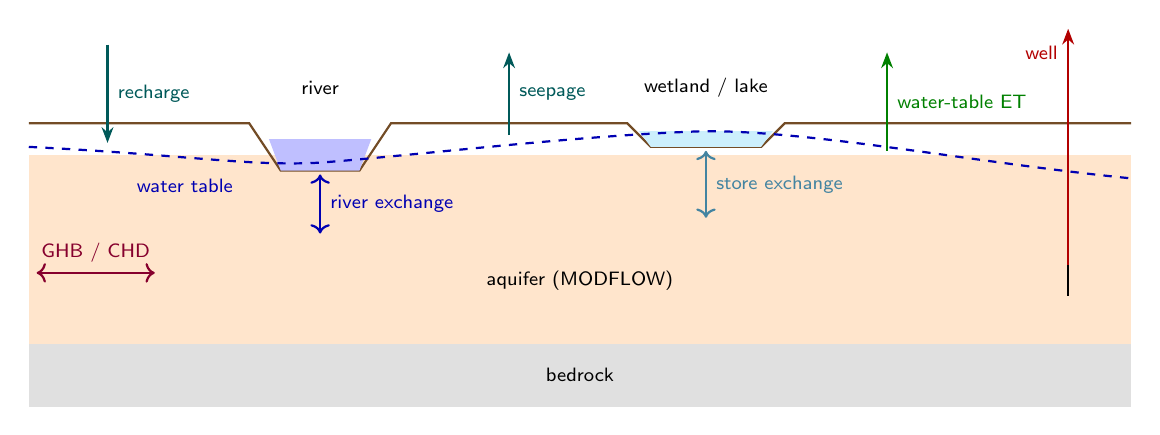
\begin{tikzpicture}[x=1cm,y=1cm,lab/.style={font=\scriptsize,align=center},ar/.style={-{Stealth[length=2mm]},thick}]
\fill[orange!20] (0,0.8) rectangle (14,3.2); \fill[black!12] (0,0) rectangle (14,0.8);
\draw[thick,brown!60!black] (0,3.6) -- (2.8,3.6) -- (3.2,3.0) -- (4.2,3.0) -- (4.6,3.6) -- (7.6,3.6) -- (7.9,3.3) -- (9.3,3.3) -- (9.6,3.6) -- (14,3.6);
\fill[blue!25] (3.05,3.4) -- (4.35,3.4) -- (4.2,3.0) -- (3.2,3.0) -- cycle; \node[lab] at (3.7,4.05) {river};
\fill[cyan!20] (7.75,3.5) -- (9.45,3.5) -- (9.3,3.3) -- (7.9,3.3) -- cycle; \node[lab] at (8.6,4.05) {wetland / lake};
\draw[dashed,blue!70!black,thick] (0,3.3) .. controls (2,3.2) and (2.8,3.05) .. (3.7,3.1) .. controls (5,3.2) and (7,3.45) .. (8.6,3.5) .. controls (10,3.5) and (12,3.1) .. (14,2.9);
\node[lab,blue!70!black,anchor=west] at (1.25,2.8) {water table};
\draw[ar,teal!70!black] (1.0,4.6) -- node[lab,right]{recharge} (1.0,3.35);
\draw[ar,teal!70!black] (6.1,3.45) -- node[lab,right]{seepage} (6.1,4.5);
\draw[ar,blue!70!black,<->] (3.7,2.95) -- node[lab,right]{river exchange} (3.7,2.2);
\draw[ar,cyan!60!black,<->] (8.6,3.25) -- node[lab,right]{store exchange} (8.6,2.4);
\draw[ar,green!50!black] (10.9,3.25) -- node[lab,right]{water-table ET} (10.9,4.5);
\draw[thick] (13.2,4.7) -- (13.2,1.4); \draw[ar,red!70!black] (13.2,1.8) -- node[lab,left,pos=0.9]{well} (13.2,4.8);
\draw[ar,purple!70!black,<->] (0.1,1.7) -- node[lab,above]{GHB / CHD} (1.6,1.7);
\node[lab] at (7,1.6) {aquifer (MODFLOW)}; \node[lab] at (7,0.4) {bedrock};
\end{tikzpicture}
\caption{The exchanges between Raven (above the water table) and MODFLOW (below). Reservoir seepage works like the store
exchange, through Raven's reservoir seepage law.}\label{fig:allexch}
\end{figure}

\section{Recharge: from Raven to the water table}\label{ch:recharge}
\subsection{Where recharge comes from}
Any Raven process that moves water into \cmd{GROUNDWATER} in a coupled HRU produces recharge --- no special process is
needed. For example, in the Liard model the percolation from the fast reservoir is sent to \cmd{GROUNDWATER} for coupled
HRUs:
\par\noindent\begin{minipage}{\linewidth}
\begin{lstlisting}
:Percolation PERC_CONSTANT FAST_RESERVOIR GROUNDWATER
  :-->Conditional HRU_GROUP IS AquiferHRUs
\end{lstlisting}
\end{minipage}\par\smallskip
At the end of a day, the \cmd{GROUNDWATER} store of HRU $k$ holds $r_k$ mm; this is the recharge of that day. Raven
counts it as water leaving Raven (its balance, Section~\ref{ch:balance}), and it is empty again at the start of the
next day.

\subsection{Volume of recharge}
\begin{equation}
V_k=\frac{r_k}{1000}\,10^{6}A_k \quad[\mathrm{m}^3],
\end{equation}
with $A_k$ the HRU area from the \cmd{.rvh} file in km$^2$ ($10^6A_k$ in m$^2$).

\subsection{Optional recharge delay}
Where the water table is deep, water takes time to cross the unsaturated zone. With the aquifer profile parameter \cmd{RECHARGE\_DELAY}~$\tau>0$ (Section~\ref{app:profile})
(days) the recharge passes through a linear reservoir $V^{\mathrm{dl}}_k$ [m$^3$] before reaching the water table:
\begin{equation}
V^{\mathrm{dl},*}_k=V^{\mathrm{dl},n}_k+V_k,\qquad V_k^{\mathrm{out}}=V^{\mathrm{dl},*}_k\left(1-e^{-\dt/\tau}\right),\qquad V^{\mathrm{dl},n+1}_k=V^{\mathrm{dl},*}_k-V_k^{\mathrm{out}} .
\end{equation}
With $\tau=0$ the delay is off and $V_k^{\mathrm{out}}=V_k$. The delay store is reported in \cmd{GWBudget.csv}, saved in
\cmd{solution.rvc} (\cmd{:GWRechargeStore}) and read back on hotstart.
\begin{example}[: recharge delay]
$\tau=60$ d, $\dt=1$ d: each day $1-e^{-1/60}=1.65\%$ of the store is released. A single 1\,000 m$^3$ pulse reaches the
water table as 16.5 m$^3$ on the first day, then less each day; after 60 days 63\% of it has arrived
(Figure~\ref{fig:curves}a).
\end{example}

\subsection{Spreading recharge over the cells}
The released volume is shared among the HRU's cells in proportion to overlap. Cells whose top cell holds a fixed head
(Section~\ref{ch:wells}) are skipped, because MODFLOW ignores recharge there:
\begin{equation}
Q^{\mathrm{rch}}_i=\sum_{k\in\mathcal{K}}\frac{V_k^{\mathrm{out}}}{\dt}\,\frac{A_{k,i}}{\sum_{j\notin\mathcal{C}}A_{k,j}}
\quad[\mathrm{m}^3/\mathrm{d}],\qquad r_i=\frac{Q^{\mathrm{rch}}_i}{|\Omega_i|}\quad[\mathrm{m/d}],
\end{equation}
where $\mathcal{C}$ are the fixed-head columns. $|\Omega_i|$ is the area of cell $i$ [m$^2$] and $r_i$ the recharge rate given to MODFLOW's RCH package, applied to the top cell of the column
(the top layer of an active column is always active). The fractions for one HRU always add up to one, so exactly $V_k^{\mathrm{out}}$
enters MODFLOW. If an HRU lies entirely on fixed-head cells, its recharge passes to that boundary and is reported in the
column \emph{recharge onto CHD cells}.
\begin{example}[: spreading recharge]
The 10 km$^2$ HRU of the Section~\ref{ch:grid} example receives 2 mm in a day: $V=0.002\times10^7=20\,000$ m$^3$. The three
cells get 8\,000, 7\,000 and 5\,000 m$^3$/d; for 4 km$^2$ cells the recharge rates are 2.0, 1.75 and 1.25 mm/d
(plus any recharge from other HRUs in the same cells).
\end{example}

\begin{figure}[!htbp]\centering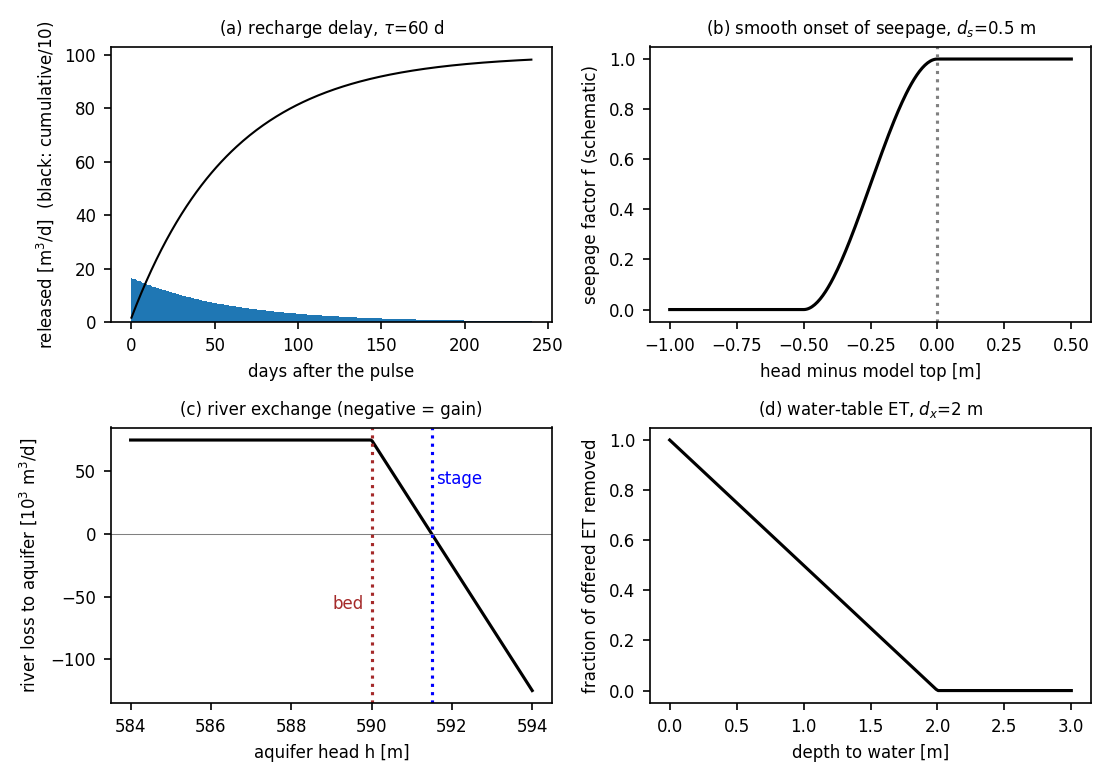
\includegraphics[width=\linewidth]{figures/fig_curves.png}
\caption{Response curves of four exchanges: (a) recharge delay reservoir after a 1\,000 m$^3$ pulse ($\tau=60$ d);
(b) seepage factor near the model top ($d_s=0.5$ m); (c) river flow against aquifer head; (d) water-table ET against
depth ($d_x=2$ m).}\label{fig:curves}\end{figure}

\begin{refcard}{recharge}
\textbf{Sources/sinks.} Moves water from \cmd{GROUNDWATER} of each coupled HRU to the aquifer (MODFLOW RCH package \cmd{RCH\_RAVEN}, top cell of each
active column), optionally through the recharge-delay store (internal to the coupling, saved in \cmd{solution.rvc}).\par\smallskip
\textbf{Constraints/notes.} In a coupled HRU \cmd{GROUNDWATER} is a pass-through: no Raven process may draw water from it (start-up error). A
process that moves water into it may return a negative flux (e.g.\ \cmd{PERC\_GR4JEXCH}): a negative recharge, taken out of the
aquifer (Section~\ref{sec:negrecharge}). The volume of each HRU is conserved exactly; recharge of HRUs lying wholly on fixed-head cells is reported
separately.\par\smallskip
\par\noindent\begin{minipage}{\linewidth}\textbf{Command syntax}
\begin{lstlisting}
# .rvi -- any process that moves water into GROUNDWATER in coupled HRUs, e.g.
:Percolation  PERC_CONSTANT  FAST_RESERVOIR  GROUNDWATER
  :-->Conditional HRU_GROUP IS AquiferHRUs
# .rvp -- optional recharge delay, per aquifer profile
:AquiferProfileParameters
  :Attributes,     RECHARGE_DELAY
  :Units,          d
  VALLEY_ALLUVIUM, 30.0
:EndAquiferProfileParameters
\end{lstlisting}
\end{minipage}\par\smallskip
\par\noindent\begin{minipage}{\linewidth}\textbf{Parameters}\par\smallskip
\begin{tabular}{>{\raggedright\arraybackslash}P{0.09\linewidth}>{\raggedright\arraybackslash}P{0.26\linewidth}>{\raggedright\arraybackslash}P{0.283\linewidth}>{\raggedright\arraybackslash}P{0.1\linewidth}>{\raggedright\arraybackslash}P{0.15\linewidth}}\toprule\hdr \hdr Symbol & Parameter & Class (where it is set) & Units & Reference\\\midrule
$r_k$ & \cmd{GROUNDWATER} & Raven state variable of HRU $k$ (filled by the chosen process) & mm & Raven state var.\\
$A_k$ & \cmd{AREA} & HRU (\cmd{:HRUs}, \cmd{.rvh}) & km$^2$ & Raven manual\\
$\tau$ & \cmd{RECHARGE\_DELAY} & aquifer profile (\cmd{:AquiferProfile\allowbreak Parameters}) & d & Sec.~\ref{app:profile}\\
$A_{k,i}$ & overlap area & computed from \cmd{:HRUGeometry} (\cmd{.rvg}) & m$^2$ & Sec.~\ref{ch:grid}\\
$|\Omega_i|$ & cell area & computed from the grid ($\Delta^2$ on a regular grid, \cmd{:GridCellSize}) & m$^2$ & Sec.~\ref{ch:grid}\\
\bottomrule\end{tabular}\end{minipage}\par\smallskip
\textbf{Outputs.} \cmd{GWBudget.csv}: \emph{Raven recharge}, \emph{MF6 recharge}, \emph{recharge delay storage}, \emph{recharge onto CHD cells};
Raven's \cmd{GROUNDWATER} storage shows each day's recharge (mm) of every HRU.
\end{refcard}

\subsection{Common questions}
\textit{Can recharge be negative?} Yes, when a process that moves water into \cmd{GROUNDWATER} returns a negative flux, such
as the GR4J exchange \cmd{PERC\_GR4JEXCH} with a positive \cmd{GR4J\_X2} (processes that take water out of \cmd{GROUNDWATER}
are refused in coupled HRUs). The negative recharge is taken out of the top active cells under the HRU. Without
\cmd{:SoilZone PHYSICAL} it is not limited by what those cells hold (a warning, once per run); with it, it is limited to what
the top cell can still give and the rest is taken back out of the soil zone (Section~\ref{sec:negrecharge}). \textit{Does recharge depend on the water table?} Not directly --- Raven decides
it. If the water table reaches the surface, the extra water returns immediately as seepage (Section~\ref{ch:seepage}), which
acts as ``rejected recharge''. With \cmd{:SoilZone PHYSICAL} rejection is explicit: recharge falling on saturated ground stays in
the soil (Section~\ref{ch:soilzone}).

\section{Seepage: groundwater returning to the surface}\label{ch:seepage}
Where the water table reaches the land surface, groundwater flows out: springs, wet meadows, seepage faces. Every active
column has a drain (MODFLOW's DRN package) at the model top that removes water whenever the water table is close to
the top, and hands it back to Raven.

\subsection{Equation}
\begin{equation}
Q^{\mathrm{seep}}_i=C^{\mathrm{drn}}_i\;f\!\left(h_i\right)\left(h_i-z_{\mathrm{top},i}+d_s\right)\ \text{ for } h_i>z_{\mathrm{top},i}-d_s,
\qquad C^{\mathrm{drn}}_i=\Lambda_s\,|\Omega_i| ,
\end{equation}
where $\Lambda_s$ [1/d] is the aquifer profile parameter \cmd{SEEPAGE\_LEAKANCE}, $|\Omega_i|$ [m$^2$] the cell area and $d_s$ [m] the aquifer profile parameter \cmd{SEEPAGE\_SMOOTHING\_DEPTH} (Section~\ref{app:profile}).
The factor $f$ rises smoothly from 0 at $d_s$ below the top to 1 at the top (Figure~\ref{fig:curves}b). Where the top cell is
thinner than $d_s$, $d_s$ is limited to its thickness (MODFLOW does not accept a smoothing interval below the cell). Without this
smoothing the drain would switch on abruptly, which makes the Newton iterations harder; with it, seepage starts gently
as the water table approaches the surface. With the soil-zone coupling (\cmd{:SoilZone PHYSICAL}, Section~\ref{ch:soilzone})
\cmd{SEEPAGE\_LEAKANCE} is not used for HRUs with a soil zone: their water exchanges with the aquifer through the soil-zone
conductance instead, and the drain serves only the HRUs without a soil zone (its conductance is scaled by their share of the cell).

\subsection{Back to Raven}
Each column's seepage is shared among the HRUs above it by overlap:
\begin{equation}
V^{\mathrm{ret}}_k=\sum_i Q^{\mathrm{seep}}_i\,\dt\,\frac{A_{k,i}}{\sum_{k'}A_{k',i}},
\end{equation}
and added to the Raven store \cmd{:SeepageReturnTo} of HRU $k$ (default: the lowest soil layer) as
$1000\,V^{\mathrm{ret}}_k/(10^{6}A_k)$ mm. HRUs without soil layers (lake, glacier or rock profiles) receive it in
\cmd{SURFACE\_WATER} instead. From there Raven's own processes take it on --- for example, the baseflow process of the
lowest soil layer carries it to the river.
\begin{example}[: seepage]
A 4 km$^2$ cell with $\Lambda_s=1$ d$^{-1}$ has $C=4\times10^6$ m$^2$/d. With the water table 0.1 m above the top and the
factor $f=1$, seepage is $4\times10^6\times(0.1+0.5)\approx2.4\times10^6$ m$^3$/d --- a large number, which is why in
practice the water table settles very close to the surface wherever the aquifer is full: the drain is a strong outlet.
\end{example}

\begin{refcard}{seepage}
\textbf{Sources/sinks.} Moves water from the aquifer (MODFLOW DRN package \cmd{DRN\_RAVEN} at the model top of every active column) to the Raven
store named by \cmd{:SeepageReturnTo} in each overlapping HRU --- by default the lowest soil layer \cmd{SOIL[$m$]}, and
\cmd{SURFACE\_WATER} for HRUs without soil layers.\par\smallskip
\textbf{Constraints/notes.} Seepage occurs only when the head is within $d_s$ of the model top; it is returned to Raven by overlap, exactly. In a step that
does not converge, MODFLOW's negative residual (more outflow booked than its inflows and storage release supply) is
withheld from seepage, river gains and store discharge in proportion; everything else MODFLOW booked is returned
(Section~\ref{sec:guard}).\par\smallskip
\par\noindent\begin{minipage}{\linewidth}\textbf{Command syntax}
\begin{lstlisting}
# .rvp
:AquiferProfileParameters
  :Attributes,     SEEPAGE_LEAKANCE, SEEPAGE_SMOOTHING_DEPTH, SOIL_ZONE_DEPTH
  :Units,          1/d,              m,                       m
  VALLEY_ALLUVIUM, 1.0,              0.5,                     0.0
:EndAquiferProfileParameters
# .rvg -- optional
:SeepageReturnTo  SOIL[2]
\end{lstlisting}
\end{minipage}\par\smallskip
\par\noindent\begin{minipage}{\linewidth}\textbf{Parameters}\par\smallskip
\begin{tabular}{>{\raggedright\arraybackslash}P{0.09\linewidth}>{\raggedright\arraybackslash}P{0.26\linewidth}>{\raggedright\arraybackslash}P{0.283\linewidth}>{\raggedright\arraybackslash}P{0.1\linewidth}>{\raggedright\arraybackslash}P{0.15\linewidth}}\toprule\hdr \hdr Symbol & Parameter & Class (where it is set) & Units & Reference\\\midrule
$\Lambda_s$ & \cmd{SEEPAGE\_LEAKANCE} & aquifer profile & 1/d & Sec.~\ref{app:profile}\\
$d_s$ & \cmd{SEEPAGE\_SMOOTHING\_DEPTH} & aquifer profile & m & Sec.~\ref{app:profile}\\
$z_{\mathrm{top}}$ & land surface $-$ \cmd{SOIL\_ZONE\_DEPTH} & \cmd{:LandSurface} (\cmd{.rvg}); aquifer profile & m & Sec.~\ref{app:profile}\\
-- & \cmd{:SeepageReturnTo} & \cmd{.rvg} option (a Raven storage state variable) & -- & Sec.~\ref{app:commands}\\
\bottomrule\end{tabular}\end{minipage}\par\smallskip
\textbf{Outputs.} \cmd{GWBudget.csv}: \emph{seepage to Raven} and \emph{returned to Raven} (equal); the receiving store in Raven's outputs.
\end{refcard}

\subsection{Choosing the leakance}
A large leakance makes the drain a strong outlet: the water table then stays within a few centimetres of the surface wherever
the aquifer is full, and seepage follows recharge closely. A small leakance lets the water table rise above the surface
(ponding in the model's sense) and delays seepage. Values of 0.1--10 d$^{-1}$ cover most cases; 1 d$^{-1}$ is the default.

\section{The soil zone and the water table}\label{ch:soilzone}
By default (\cmd{:SoilZone CONCEPTUAL}) Raven's soil and the aquifer meet only through recharge and the seepage drain:
Raven's soil never sees the water table. With \cmd{:SoilZone PHYSICAL} the water table can rise into chosen Raven soil
layers, saturated soil drains to the aquifer, recharge stops where the ground is saturated, and a full soil zone
overflows to the surface --- the arrangement of GSFLOW \cite{markstrom2008gsflow}, where the soil zone sits above the
MODFLOW domain.

\begin{plain}
Think of the soil layers you name (for example \cmd{SOIL[0]} and \cmd{SOIL[1]}) as the top of the aquifer, owned by
Raven. MODFLOW starts below them. When the water table climbs to the bottom of the soil, it carries on rising inside the
soil layers; rain falling on that saturated ground cannot soak down any more and stays in the soil, and once the soil is
full the extra water runs off. When it is dry, saturated soil drains down into the aquifer again. On a slope this
happens first at the bottom of the hill, because Raven checks the ground height at many points in each cell.
\end{plain}

\subsection{Who owns which depth}
Raven owns the soil zone \cmd{SOIL[0]}\,\dots\,\cmd{SOIL[$M-1$]} of every coupled HRU with soil; MODFLOW owns everything
below. The soil-zone thickness is $d_{\mathrm{sz},k}=\sum_mH_m$ (the thicknesses $H_m$ of those layers in the HRU's soil profile) and the
model top of column $i$ is
\begin{equation}
z_{\mathrm{top},i}=z_{\mathrm{land},i}-\frac{\sum_kA_{k,i}\,d_{\mathrm{sz},k}}{\sum_kA_{k,i}},
\end{equation}
so the soil pore space is not counted twice. HRUs without soil (lake, water, glacier and rock types) have $d_{\mathrm{sz},k}=0$ and
keep the seepage drain (Section~\ref{ch:seepage}); \cmd{SOIL\_ZONE\_DEPTH} and, for soil-zone HRUs,
\cmd{SEEPAGE\_LEAKANCE} are not used. Recharge must leave the soil zone from its bottom layer \cmd{SOIL[$M-1$]}
(start-up check), as in GSFLOW, where gravity drainage leaves the bottom of the soil zone.

\subsection{Columns: one soil zone per HRU and cell}
An HRU usually spans several cells, and the water table differs between them. The soil zone of HRU $k$ is therefore kept
as one \emph{column} per overlapping cell (GSFLOW's gravity reservoir per HRU--cell), including cells with a specified
head (Section~\ref{sec:szchd}), plus one column for the rest of the HRU (outside the grid). The column of HRU $k$ in cell $i$ has its own soil water $\phi_{k,i,m}$ [mm] in every layer $m$;
Raven's \cmd{SOIL[$m$]} of the HRU is their area-weighted mean, so Raven's processes see one soil store per HRU, as
without the soil zone (or, with
\cmd{:SoilZoneClasses}, each class of its columns separately; Section~\ref{sec:szclasses}). Between
exchanges Raven changes the HRU totals, and the changes are shared among the columns as the processes would have made
them there: the recharge leaves the columns as the percolation takes it (every column alike for \cmd{PERC\_CONSTANT},
from free water for a drainage), percolation between soil layers stays in its column, evaporation is taken alike on
every column, and rain falls alike on every column, what a full column cannot take overflowing to
\cmd{SURFACE\_WATER}. The columns are saved in
\cmd{solution.rvc} (\cmd{:GWSoilZoneColumns}). At the start (no hotstart) every column is filled up to the initial water
table of its cell.

\subsection{Soil water level}
For one column (indices $k,i$ dropped), layer $m$ (\cmd{SOIL[$m$]}, $m=M-1$ at the bottom of the soil zone) holds $\phi_m$
between field capacity $\phi_{\mathrm{fc},m}=\phi_{\max,m}S_{\mathrm{fc},m}$ and capacity
$\phi_{\max,m}=1000H_m\eta_m(1-\mathit{SF}_m)$ [mm], with porosity $\eta_m$ and stone fraction $\mathit{SF}_m$
(\cmd{POROSITY}, \cmd{STONE\_FRAC}). Its saturated share is
$\chi_m=\min(\max((\phi_m-\phi_{\mathrm{fc},m})/(\phi_{\max,m}-\phi_{\mathrm{fc},m}),0),1)$ and the saturated thickness of the
column is
\begin{equation}
b^{\mathrm{sz}}=\sum_{m=0}^{M-1}H_m\,\chi_m\prod_{m'>m}\chi_{m'}\quad[\mathrm m]:
\end{equation}
water up to field capacity fills the deficit without raising the level, free water raises it with the drainable porosity
$S_d=\eta(1-\mathit{SF})(1-S_{\mathrm{fc}})$, and the level rises through a layer once the layers below are full. The cell's land
surface is sampled at $N_g$ points $g$ (\cmd{:SoilZoneSubgrid}; 25 by default) with soil-zone bases
$z_{b,g}=z_{\mathrm{land},g}-d_{\mathrm{sz},k}$. The column's free water stands at one flat level $h^{\mathrm{sz}}$ over these points (as MODFLOW's
head is flat over the cell), defined by $\frac1{N_g}\sum_g\min(\max(h^{\mathrm{sz}}-z_{b,g},0),d_{\mathrm{sz},k})=b^{\mathrm{sz}}$. Section~\ref{sec:szslope} shows how this handles sloping and irregular land.

\subsection{Exchange}
A point comes into hydraulic contact with the aquifer as the water table rises through the depth $d_s$
(\cmd{SEEPAGE\_SMOOTHING\_DEPTH}) below its base, the capillary fringe, and is fully in contact at its base:
$w_g=\sigma((h_i-z_{b,g})/d_s+1)$ with $\sigma(x)=3x^2-2x^3$ on $(0,1)$, 0 below and 1 above. (Full contact at the base,
because MODFLOW's top cell ends there: above it the soil's storage must take over at once.) The exchange into the
aquifer is
\begin{gather}
q^{\mathrm{sz}}_{k,i}=\frac{C^{\mathrm{sz}}_{k,i}}{N_g}\sum_gw_g\Big(\min(\max(h^{\mathrm{sz}},z_{b,g}),z_{b,g}+d_{\mathrm{sz},k})-\max(h_i,z_{b,g})\Big),\\
C^{\mathrm{sz}}_{k,i}=\frac{A_{k,i}}{\dfrac{H_{M-1}}{2\,K_{\mathrm{sat},M-1}/1000}+\dfrac{b_i}{2\,K_{v,i}}}\quad[\mathrm{m^2/d}],
\end{gather}
positive into the aquifer: the soil--aquifer conductance $C^{\mathrm{sz}}_{k,i}$ is the series resistance of half the bottom soil-zone layer
($K_{\mathrm{sat},M-1}$ = \cmd{HYDRAUL\_COND} [mm/d]) and half the top active aquifer cell (thickness $b_i$, vertical conductivity
$K_{v,i}$). With a single point and the water table above the base this is simply $q^{\mathrm{sz}}=C^{\mathrm{sz}}(z_b+b^{\mathrm{sz}}-h_i)$: water flows up
when the water table is above the soil water level and down when it is below; a point in contact while the water table
is still below its base only drains the water standing in its soil. The exchange goes to MODFLOW through a GHB package \cmd{SZX\_RAVEN} (one entry per
HRU--cell column, plus a WEL package \cmd{SZQ\_RAVEN} for the part of the boundary that would lie below the cell bottom).
GHB rather than RIV or DRN because the exchange runs both ways and must stop where the water table is below the soil
(through $F$) without adding a second drainage path next to Raven's percolation.

\subsection{Rejected recharge, overflow and evaporation}
The HRU's recharge goes to the cells of the columns that gave it up, not by area, so drainage from saturated columns at
the foot of a slope is not sent up the slope. Of each column's share, the saturated fraction $F=\frac1{N_g}\sum_g\sigma((h_i-z_{b,g})/d_s)$ --- the points where the
water table has risen into the soil --- is \emph{rejected}: it stays in the column instead of reaching MODFLOW, which
receives $(1-F)$ (Section~\ref{ch:recharge}). \emph{Raven recharge} in \cmd{GWBudget.csv} therefore includes water that is
rejected and returned; the net recharge is \emph{MF6 recharge}. Water that does not fit into a full
column overflows to the HRU's \cmd{SURFACE\_WATER} and is routed the same day (saturation-excess runoff and
exfiltration). Water-table ET is reduced by $(1-\bar F_i)$ of the cell, because saturated soil already evaporates in
Raven; its extinction depth counts from the ground above the soil zone, as without a soil zone (Section~\ref{ch:et}).

\subsection{Sloping and irregular land}\label{sec:szslope}
Partial saturation is handled at two scales. \emph{Between cells}, MODFLOW gives every cell its own head and its own
top and bottom (the layers need not be horizontal: the generated model's top follows the land, one soil-zone thickness below it, and an existing model
keeps its own geometry), and every HRU--cell link has its own column; so along a slope each column sees its own water
table, and an HRU can be saturated at its foot and dry at its top. \emph{Within a cell}, MODFLOW's head is one flat
level, but the land is not. The $N_g$ DEM points of the cell carry the land's relief into the soil zone: each point has its
own soil-zone base $z_{b,g}$, so a water table rising into a sloping or bumpy cell saturates the soil first at the low
points and only later at the high ones. Figure~\ref{fig:szsubgrid} shows one cell with the formulas of this chapter:
\begin{itemize}
\item (a) The water table is below every base: no point is in contact ($w_g=0$), $F=0$, and the recharge reaches the
aquifer in full (through the unsaturated column, Section~\ref{sec:szvadose}, when \cmd{:SoilZoneVadose} is \cmd{RICHARDS}, \cmd{KINEMATIC} or \cmd{LAG}).
\item (b) The water table has risen into the soil at the low end of the cell only. There the soil is saturated
($F=0.40$: 40\,\% of the recharge is rejected and stays in the soil), while the high end still drains freely. At rest the
soil water level equals the water table and nothing is exchanged.
\item (c) After rain the soil water stands above the water table ($h^{\mathrm{sz}}>h_i$): the points in contact drain into the aquifer
(arrows, $q>0$). The point at 45~m holds water above its base but is not yet in contact (the water table is more than
$d_s$ below it); that water is perched and leaves by percolation, as recharge.
\item (d) A high water table below a drier soil ($h_i>h^{\mathrm{sz}}$) pushes water up into the soil ($q<0$); at the lowest points
the water table is above the land. All four states use the same $F$, $w_g$ and $q$; nothing is switched.
\end{itemize}
The bottom panel shows how $F$, the mean contact $\bar w$ and the saturated thickness at rest grow with the water table:
each point adds a smooth step (width $d_s$), so the curves are continuous and monotone for any relief, which keeps
MODFLOW's Newton iterations smooth. With \cmd{:SoilZoneSubgrid 1} each cell has a single point and $F$ is one step.

\begin{figure}[!htbp]\centering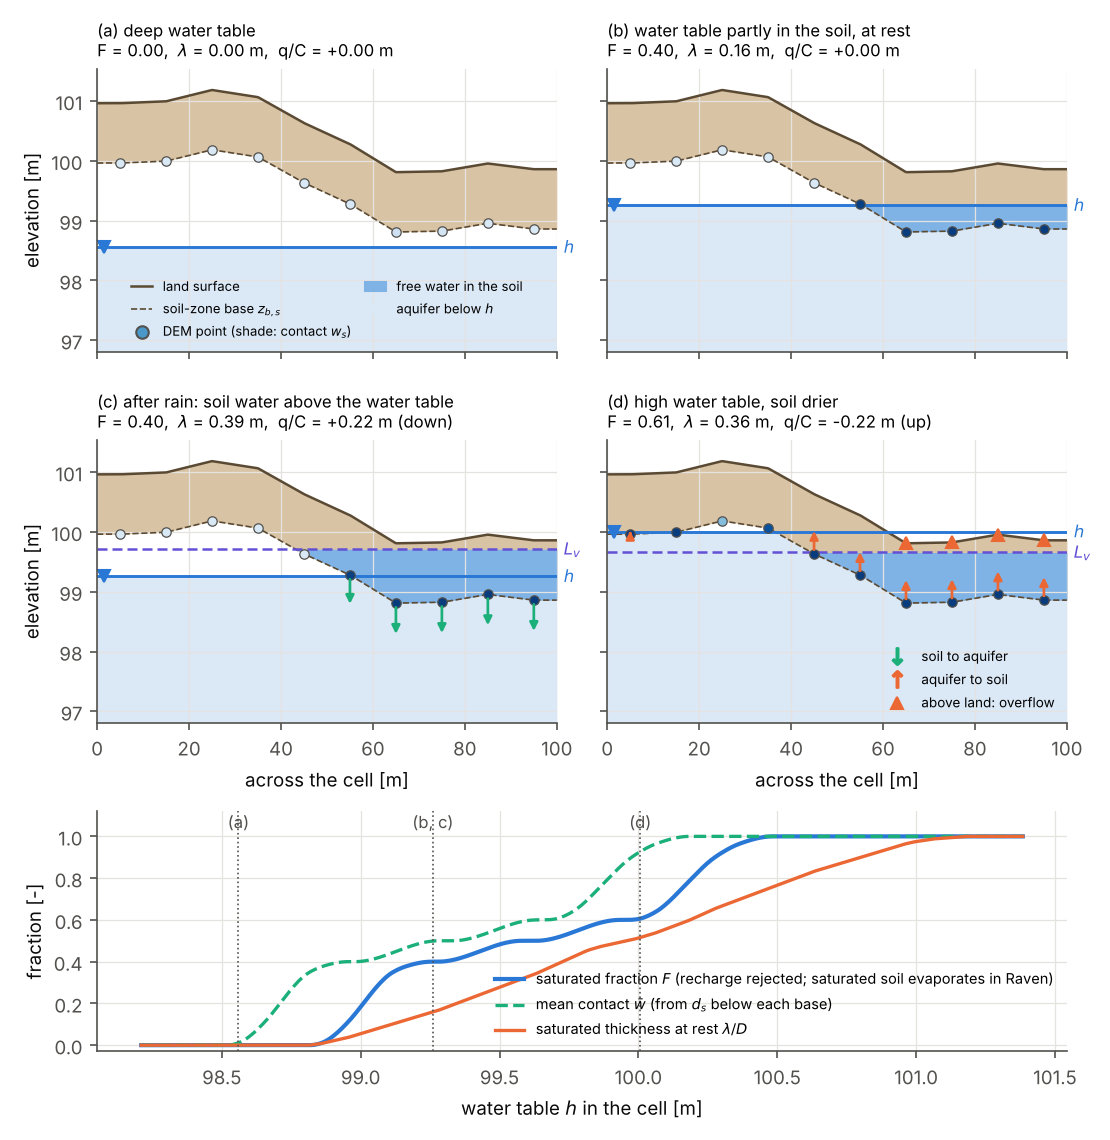
\includegraphics[width=\linewidth]{figures/fig_sz_subgrid.png}
\caption{One 100~m cell with irregular land ($d_{\mathrm{sz}}=1$~m, $d_s=0.3$~m), seen along a transect of its DEM points (circles at the
soil-zone base, shaded by their contact weight $w_g$). (a)--(d): four states of the water table $h$ and soil water level
$h^{\mathrm{sz}}$, with the saturated fraction $F$, the saturated thickness $b^{\mathrm{sz}}$ and the exchange $q/C$ (positive into the aquifer);
arrows show each point's share of the exchange. Bottom: $F$, the mean contact $\bar w$ and $b^{\mathrm{sz}}/d_{\mathrm{sz}}$ at rest
($h^{\mathrm{sz}}=h$) against the water table. Computed with the model's formulas
(script \texttt{make\_sz\_subgrid\_figures.py} in the manual's figures folder).}\label{fig:szsubgrid}\end{figure}

Figure~\ref{fig:szhillslope} shows a coupled run: the hillslope of test HS1/HS2 (ten 100~m HRUs on a 0.5\,\% slope) with a hump
at 300~m and hollows at 620 and 850~m added to its DEM, 25 points per cell and $d_s=0.1$~m. The water table is a step
per cell (MODFLOW's flat head). Under rain the saturated area spreads up from the foot of the slope and from the
hollows; over the hump (HRUs 3--4) and near the top (HRU 2) the cells are only partly saturated for months
($0<F<1$). Water moves down the slope in the aquifer: it rises into the soil of the lower cells, which fill and
overflow to surface water (saturation-excess runoff and exfiltration). After the rain the saturated area retreats
downslope, the hollows last. (In the closed aquifer of test HS2 the overflow stops upslope when the rain does, but the water
still draining from upslope seeps out at the toe for the rest of the run, about 174~m$^3$/d on day 300, as in the
MODFLOW-only reference; HS2 checks that the HRUs that drain lose their saturation and that the toe follows a recession.) The run closes every balance of Section~\ref{sec:accsz} to $10^{-9}$ or better (Section~\ref{sec:vszbasic}).

\begin{figure}[!htbp]\centering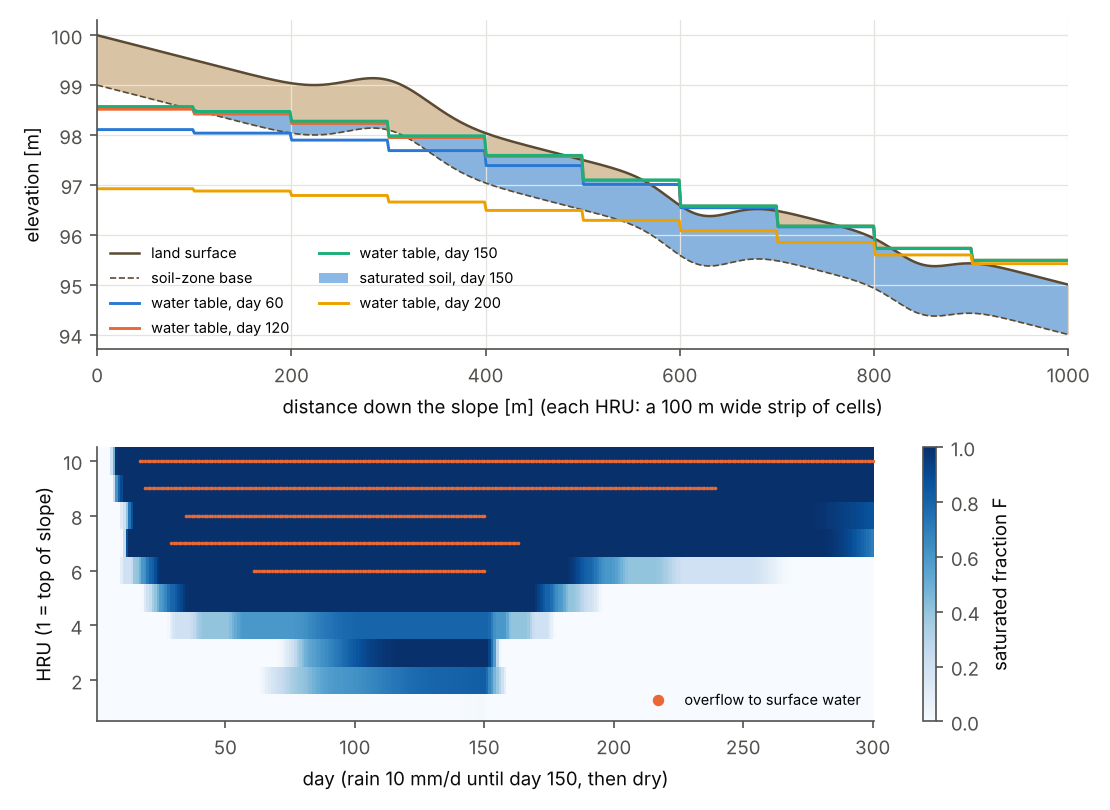
\includegraphics[width=\linewidth]{figures/fig_sz_hillslope.png}
\caption{Coupled hillslope with irregular land (rain 10~mm/d for 150 days, then dry). Top: land surface, soil-zone base and
the water table of each cell on four days; shaded, the saturated soil on day 150. Bottom: saturated fraction $F$ of each
HRU over time (1 = top of the slope), with the days on which the HRU overflows to surface water.}\label{fig:szhillslope}\end{figure}

What the sub-grid closure does not resolve: a column keeps one flat soil water level, so within a cell the soil water is
spread over the points at once, and the column overflows only when it is full, that is when $h^{\mathrm{sz}}$ reaches the highest
land point. A water table above the land at the low points of a partly filled cell (panel (d)) therefore pushes water into the higher parts of the column instead of running off there;
seepage faces smaller than a cell need smaller cells. Between cells, soil water moves only through the aquifer.

\subsection{Solving soil and aquifer together}
Within a day the soil column and the aquifer must agree. For given heads each column is solved implicitly
(backward Euler) for its change $\Delta\phi$ [mm]:
\begin{equation}
\Delta\phi+\frac{1000\,\dt}{A_{k,i}}\,q^{\mathrm{sz}}_{k,i}\big(b^{\mathrm{sz}}(\phi^*+\Delta\phi),h_i\big)=0,
\end{equation}
where $A_{k,i}$ [m$^2$] is the column area and $\phi^*$ its water after Raven's processes plus the rejected recharge. The left side
increases strictly with $\Delta\phi$, so there is exactly one solution (found by Brent's method); if it lies beyond full, the
column fills and the rest overflows. MODFLOW receives each column as a linear boundary that reproduces this exchange at
the current head and its slope, including the column's own response (a Robin interface condition). After MODFLOW's
outer iterations the columns are solved again with the new heads --- after every one of the first five, and afterwards
after every iteration on which MODFLOW has converged, but not in MODFLOW's last tenth of its iteration limit --- until
the soil levels change by less than the head tolerance and the total exchange by less than the flow tolerance
(\cmd{:SoilZoneIteration}). The flows Raven applies are always
the ones MODFLOW booked, so no water is created or lost even on a step whose interface did not converge (reported in
\cmd{Raven\_errors.txt}). A boundary MODFLOW keeps without further updates (explicit mode, \cmd{:SoilZoneIteration 0},
and the last update before the interface freezes) may not take more from a column than it holds: where the soil
drains, its slope is limited by the column's free water; where water rises into the soil, the line becomes a smoothed
drain that stops at its zero-flow level instead of turning into flow out of a column that has no water to give.

While the water table is below the soil base the exchange does not depend on the head (a rate: the soil drains to its
base), and MODFLOW would have no way to return water to the soil if the head rose past the base during its solve: the
excess would go into the elastic storage above the cell top, heads metres above ground in one iteration. Such links therefore also get a drain in \cmd{SZD\_RAVEN} at the lowest base point of the cell, smoothed
over $d_s$, with the link's conductance $C$ and at least the conductance that carries the link's inflow (its rate and
its share of the cell's recharge) out over one soil-zone thickness, $\max\big(C,\,Q_{\mathrm{in}}/d_{\mathrm{sz},k}\big)$. Below the
base it carries nothing, so a converged step that stays below the base is unchanged; above it the water goes back to
the soil as exchange (aquifer to soil zone), as the next interface update would send it.

\begin{example}[: water table rising into the soil]
Two soil-zone layers of 0.5 m with $\eta=0.4$, $\mathit{SF}=0$, $S_{\mathrm{fc}}=0.5$: $\phi_{\max}=200$ mm, $\phi_{\mathrm{fc}}=100$ mm and
$S_d=0.2$ in each. The top aquifer layer has $S_y=0.2$ and receives 10 mm/d of recharge. Below the soil the water table
rises $10/0.2=50$ mm/d. When it reaches the soil base the recharge is rejected and stays in the soil, where it raises
the soil water level by $10/0.2=50$ mm/d as well; the 400 mm of capacity hold the remaining 200 mm of free water after 20
more days, after which all recharge overflows (test CT1, Section~\ref{sec:vszbasic}: 49.95~mm/d, full on day 41). Exchange: with
$K_{\mathrm{sat}}=100$ mm/d, a 10 m top cell with $K_v=1$ m/d and a 100$\times$100 m column,
$C^{\mathrm{sz}}=10^4/(0.5/0.2+10/2)=1\,333$ m$^2$/d. Soil water 0.2 m and water table 0.1 m above the base ($F=1$) give
$q^{\mathrm{sz}}=1\,333\times0.1=133$ m$^3$/d into the aquifer, 13 mm/d over the column.
\end{example}

\subsection{Every position of the water table}\label{sec:szregimes}
The water table can stand anywhere relative to the soil zone, and it moves through all of these positions in the
course of a year. Figure~\ref{fig:szregimes} shows what carries the water in each; the coupling switches between them
smoothly, column by column and step by step, without any setting.
\begin{figure}[!htbp]\centering% Positions of the water table relative to the soil zone and what carries the water in each
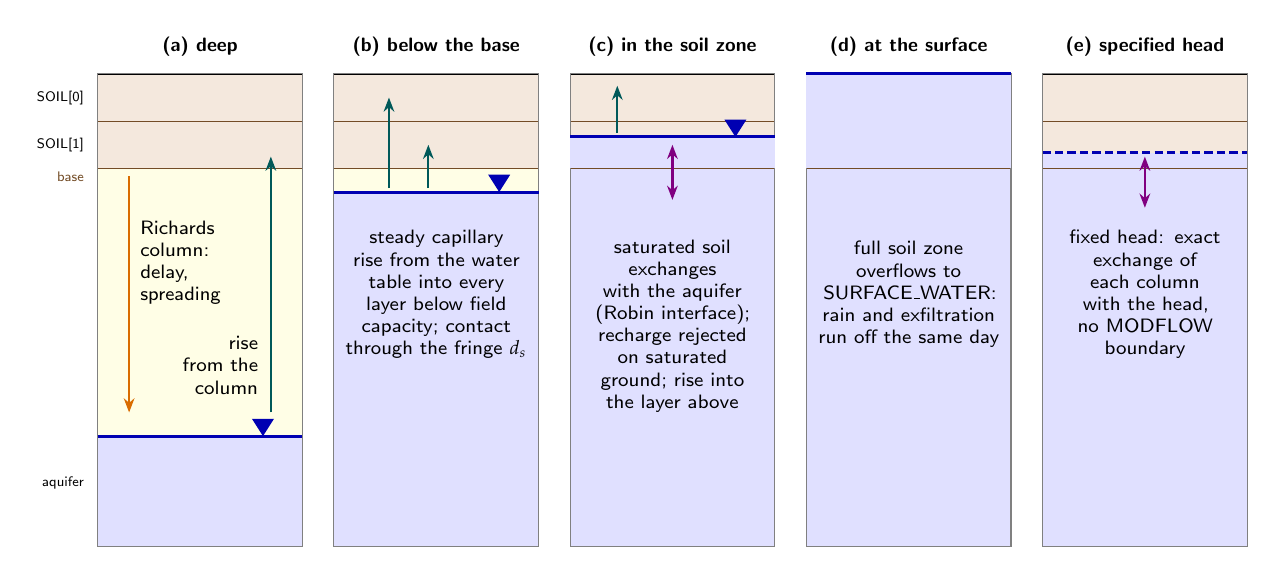
\begin{tikzpicture}[font=\sffamily\scriptsize,x=1mm,y=1mm,
  soil/.style={fill=brown!18,draw=brown!60!black,line width=0.4pt},
  unsat/.style={fill=yellow!10,draw=none},
  sat/.style={fill=blue!12,draw=none},
  wt/.style={blue!70!black,line width=1.1pt},
  base/.style={brown!60!black,dashed,line width=0.6pt},
  up/.style={-{Stealth[length=1.8mm]},line width=0.8pt,teal!70!black},
  dn/.style={-{Stealth[length=1.8mm]},line width=0.8pt,orange!85!black},
  lab/.style={align=center,text width=23mm,inner sep=1pt}]
% one panel: x offset #1, water-table elevation #2 (land 60, soil base 48, soil layers 48-54-60)
\newcommand{\panel}[2]{%
  \fill[sat] (#1,0) rectangle (#1+26,#2);
  \fill[unsat] (#1,#2) rectangle (#1+26,48);
  \draw[soil] (#1,48) rectangle (#1+26,54);
  \draw[soil] (#1,54) rectangle (#1+26,60);
  \draw[base] (#1,48) -- (#1+26,48);
  \draw[line width=0.8pt] (#1,60) -- (#1+26,60);
  \draw[gray] (#1,0) rectangle (#1+26,60);}
% (a) deep water table
\panel{0}{14}
\draw[wt] (0,14) -- (26,14); \fill[blue!70!black] (21,14) -- ++(-1.4,2.2) -- ++(2.8,0) -- cycle;
\draw[dn] (4,47) -- (4,17); \node[lab,text width=13mm,align=left,anchor=west] at (5,36) {Richards column: delay, spreading};
\draw[up] (22,17) -- (22,49.5); \node[lab,text width=12mm,align=right,anchor=east] at (20.8,23) {rise from the column};
% (b) just below the soil base
\panel{30}{45}
\draw[wt] (30,45) -- (56,45); \fill[blue!70!black] (51,45) -- ++(-1.4,2.2) -- ++(2.8,0) -- cycle;
\draw[up] (37,45.5) -- (37,57); \draw[up] (42,45.5) -- (42,51);
\node[lab] at (43,32) {steady capillary rise from the water table into every layer below field capacity; contact through the fringe $d_s$};
% (c) in the soil zone
\panel{60}{52}
\fill[sat] (60,48) rectangle (86,52); \draw[wt] (60,52) -- (86,52); \fill[blue!70!black] (81,52) -- ++(-1.4,2.2) -- ++(2.8,0) -- cycle;
\draw[up] (66,52.5) -- (66,58.5);
\draw[{Stealth[length=1.8mm]}-{Stealth[length=1.8mm]},line width=0.8pt,violet] (73,44) -- (73,51);
\node[lab] at (73,28) {saturated soil exchanges with the aquifer (Robin interface); recharge rejected on saturated ground; rise into the layer above};
% (d) at the land surface
\panel{90}{60}
\fill[sat] (90,48) rectangle (116,60); \draw[wt] (90,60) -- (116,60);
\node[lab] at (103,32) {full soil zone overflows to SURFACE\_\-WATER: rain and exfiltration run off the same day};
% (e) specified head
\panel{120}{50}
\fill[sat] (120,48) rectangle (146,50); \draw[wt,dash pattern=on 3pt off 1.5pt] (120,50) -- (146,50);
\draw[{Stealth[length=1.8mm]}-{Stealth[length=1.8mm]},line width=0.8pt,violet] (133,43) -- (133,49.5);
\node[lab] at (133,32) {fixed head: exact exchange of each column with the head, no MODFLOW boundary};
% labels
\foreach \x/\t in {0/(a) deep,30/(b) below the base,60/(c) in the soil zone,90/(d) at the surface,120/(e) specified head}{
  \node[font=\sffamily\bfseries\scriptsize,anchor=south] at (\x+13,61) {\t};}
\node[anchor=east,font=\sffamily\tiny] at (-0.5,57) {SOIL[0]}; \node[anchor=east,font=\sffamily\tiny] at (-0.5,51) {SOIL[1]};
\node[anchor=east,font=\sffamily\tiny,brown!60!black] at (-0.5,47) {base}; \node[anchor=east,font=\sffamily\tiny] at (-0.5,8) {aquifer};
\end{tikzpicture}

\caption{Where the water table can be and what moves the water in each case. (a) Deep: recharge crosses an unsaturated
column solved with Richards' equation (\cmd{:SoilZoneVadose RICHARDS}), which delays and spreads it; the column also
feeds capillary rise into the soil zone. (b) Within the column's minimum length below the soil base: no column; the
exchange starts through the fringe $d_s$, and capillary rise from the water table reaches the layers above. (c) In the
soil zone: the saturated soil exchanges with the aquifer, recharge on saturated ground is rejected, capillary rise
continues into the layers above the water table. (d) At the surface: the full soil zone overflows. (e) Over a specified
head: each column exchanges with the fixed head exactly.}\label{fig:szregimes}
\end{figure}

\begin{plain}
When the water table is deep, rain that drains out of the soil takes days to weeks to reach it, and arrives spread
out; Raven follows that trip through the dry ground below the soil. When the water table is shallow, it also
works the other way: dry soil pulls water up from it, so plants and evaporation keep drawing on groundwater after the
rain stops. Both are computed from the soil's own retention curve, not from a fitted delay or a rate you set.
\end{plain}

\subsection{The unsaturated column}\label{sec:szvadose}
With \cmd{:SoilZoneVadose RICHARDS} every exchange column whose water table lies more than
$L_{\min}=0.05$~m below its soil-zone base gets an unsaturated column from the base $z_b$ (the cell's mean base; with
\cmd{:SoilZoneVadoseClasses}, one column per depth class of its DEM samples, Section~\ref{sec:vzclasses}) down to the
water table $h$ (the head of the top active cell at the start of the step). Its water content $\theta(z,t)$ follows
the mixed form of Richards' equation \cite{celia1990}, $z$ upward,
\begin{equation}
\frac{\partial\theta}{\partial t}=\frac{\partial}{\partial z}\Big[K(\psi)\Big(\frac{\partial\psi}{\partial z}+1\Big)\Big],
\end{equation}
with Campbell's retention curve \cite{campbell1974} and its Hutson--Cass parabola near saturation \cite{hutson1987},
\begin{equation}
\psi(S)=\begin{cases}-\psi_a\,S^{-b}, & S\le S_i,\\[2pt] -\psi_i\sqrt{\dfrac{1-S}{1-S_i}}, & S>S_i,\end{cases}\qquad
S=\frac{\theta}{\theta_s},\quad S_i=\frac{2b}{1+2b},\quad \psi_i=\psi_a S_i^{-b},\qquad K=K_s\,S^{2b+3}
\end{equation}
(continuous with a continuous slope at $S_i$, so the Newton iteration never meets a kink). The material of each depth
is the aquifer class of the MODFLOW layer there: $K_s$ = \cmd{K\_VERT}, $\theta_s$ = \cmd{POROSITY}, $b$ = \cmd{CLAPP\_B},
$\psi_a$ = \cmd{AIR\_ENTRY\_PRESSURE} [m], $S_y$ = \cmd{SPEC\_YIELD} (Section~\ref{app:class}). Layers of different
classes form a layered column, so a slowly permeable layer holds a perched saturated zone above it.

\paragraph{Discretization.} Each column has at most $N$ finite volumes (\cmd{:SoilZoneVadose RICHARDS} $\epsilon$ $N$;
$N=16$ by default; a column shorter than $N\times5$~cm has one per 5~cm, at least 3), growing geometrically by 1.3 from
both ends towards the middle, to at most $1.3^8=8.2$ times the end volumes: a column of length $L$ with $N=16$ has end
volumes of $L/48$ (5~cm for $L=2.4$~m, 21~cm for 10~m) and middle ones of $0.13L$; from $N=19$ on the extra volumes fill
the middle at the largest thickness, about $L/(N-10)$, so raising $N$ refines the whole column. Each Raven step
is divided into substeps, each solved by backward Euler in the mixed (mass-conservative) form with Newton's method on
the tridiagonal system; a substep is accepted when no cell changes its content by more than $\epsilon$ (0.02 by
default) and halved otherwise, and the next one grows by half when Newton converged quickly. Newton's updates are
damped in logarithmic steps towards saturation (a dry node recovers in a few iterations), and once the top has
saturated the next substeps try the saturated top first; an air-dry top under an upward demand likewise switches to
its driest suction ($10^5$~m), and the demand it cannot supply is returned to the soil zone. Upward flow through the
bottom comes out of the cell holding the water table (Section~\ref{sec:szcaprise}: the top cell, or through
\cmd{SZW\_RAVEN} a cell below it when the top cell has dried); out of a cell near drying it is scaled down with that
cell's water, and where no cell has water there is none: even a trace of negative recharge into a dry cell makes
MODFLOW's Newton iteration oscillate (on Liard it quadrupled the outer iterations). The bottom boundary is
$\psi=0$ at the water table. The top boundary is the unsaturated share of the column's recharge (Section~\ref{ch:recharge}),
$q_{\mathrm{top}}=(1-F)R_{k,i}/A_{k,i}$, less the capillary rise into the soil zone; when the top cell saturates it switches to
$\psi=0$ and what it cannot take is \emph{rejected}: it returns to the soil-zone column as rejected recharge, exactly
like recharge on saturated ground. The flux into MODFLOW is taken from the column's storage change,
\begin{equation}
q_{\mathrm{bot}}=q_{\mathrm{top}}-\frac{1}{\dt}\sum_i\big(\theta_i^{n+1}-\theta_i^{n}\big)\Delta z_i,
\end{equation}
so the column conserves water to round-off whatever the Newton tolerance; $q_{\mathrm{bot}}A_{k,i}$ replaces the column's
share of the recharge in \cmd{RCH\_RAVEN}. The column is solved once per Raven step, before MODFLOW's solve, with the
water table of the start of the step.

\paragraph{Steady start.} With \cmd{:SoilZoneVadoseInitialFlux} $q$ (a cold start) every column starts at the steady
state of these finite volumes for the flux it receives in the first step, $(1-F)\,q$, $F$ the saturated fraction of its
class at the initial head: every face carries that flux, solved node by node from the water table up (a layer whose
$K_s$ is below the flux holds a saturated, perched zone above it). Where the flux exceeds what the column can pass with
$\psi=0$ at its top, that profile would put positive pressure at the top; the column then starts at the backed-up steady
state instead, for the largest flux $f$ it passes with a saturated top, and its top rejects the rest from the first step
(Raven warns, with the number of such columns). Either way the start is steady to the solver's tolerance: the first
step's outflow equals its inflow and the storage does not change (\cmd{test\_vz\_initial.py} VI1, VI5, VI6).

\paragraph{A moving water table.} The water table's own rise and fall is MODFLOW's: its specific yield stores and
releases the water. The column therefore carries only what differs from the hydrostatic (equilibrium) profile above
the water table, $\theta_{\mathrm{eq}}(z)=\theta\big(\psi=-(z-h)\big)$: water in transit to the water table, and
deficits left by evaporation and capillary rise (\emph{unsaturated zone storage}
$=\sum_i(\theta_i-\theta_{\mathrm{eq},i})\Delta z_i$). At the start of every step the column's bottom moves to the new
water table: the excess keeps its elevation, the equilibrium follows the water table, and where the water table has
risen the excess below it joins the aquifer as recharge this step (\emph{unsaturated zone to aquifer} includes it);
where it has fallen, the new cells start at equilibrium, and the water they take comes out of the cell holding the
water table, at most what that cell can give in the step (above; the column's bottom then follows more slowly). The
same limit applies to the deficit below a risen water table in a column dried by evaporation or capillary rise. (Opening them at $\theta_s-S_y$, what MODFLOW's specific yield
leaves behind, would leave a dry band next to the water table that refills from the aquifer at once, a feedback that
diverges with explicit coupling wherever $S_y$ exceeds the drainable porosity the retention curve implies near the
water table.) A node that the move leaves above its porosity, or drier than air-dry, is clipped and the difference
exchanged with the aquifer. A rising water table releases at most what MODFLOW stores for that rise, $S_y\Delta h$ per
unit area (integrated over the layers the rise crosses), in one step, and no more than the room the top cell has left
above the water table ($S_y$ integrated from the head up to the cell's top or the column's base, whichever is lower); the column's bottom then follows more slowly and releases the rest in the next steps. With
$S_y$ consistent with the retention curve this never binds; with $S_y$ well below the drainable porosity a rising water
table would otherwise release more from the column at each step than the last (a feedback with gain $(\theta-\theta_{\mathrm{eq}})/S_y>1$),
and Raven warns at start-up when $S_y$ and $\theta_s-\theta(\psi=-1\text{ m})$ of a class differ by more than a factor 2.
When the water table rises to within $L_{\min}$ of the base the column disappears (rule (ii) below) and the
soil zone's contact exchange (above) takes over; when it falls again the column reappears at equilibrium. The columns
are saved in \cmd{solution.rvc} (\cmd{:GWVadoseColumns}; with depth classes \cmd{:GWVadoseClassColumns}).

\paragraph{Water handed back to the soil zone.} Two rules send column water to the soil zone instead of the aquifer.
Both book it as \emph{rejected recharge}: it reaches the soil-zone layers as recharge on saturated ground does.
\begin{description}
\item[Rule (i): ground saturated during the step.] The column is solved with the water table of the start of the step,
but MODFLOW's head can rise during the step onto ground that was unsaturated at its start: the saturated fraction of the
column's ground rises from $F_0$ to $F(h)$. The column's outputs on that ground (its flux into MODFLOW and the excess a
rising water table releases) go back to the soil zone, $R_q\min\big(\max(F(h)-F_0,0),\,1-F_0\big)$, with $R_q$ the
column's outputs divided by $1-F_0$. A column whose ground was wholly saturated at the start of the step ($F_0=1$) hands
back all its outputs. With the interface iteration the share follows the head of each iteration
(Section~\ref{sec:szinterface}); in explicit coupling only the case $F_0=1$ applies. With depth classes the rule applies
class by class (Section~\ref{sec:vzclasses}).
\item[Rule (ii): a vanishing column.] A column that disappears because the water table rose to within $L_{\min}$ of its
base releases to the aquifer at most what MODFLOW stores for the rise (the limit $S_y\Delta h$ above); the rest of its
water goes back to the soil zone.
\end{description}
In \cmd{GWBudget.csv} the water handed back is part of \emph{rejected recharge}. It is subtracted from \emph{unsaturated
zone inflow} (both rules) and from \emph{unsaturated zone to aquifer} (rule (i), whose water was among the column's
outputs), so the column identity $\Delta V^{\mathrm{uz}}=V^{\mathrm{uz}}_{\mathrm{in}}-V^{\mathrm{uz}}_{\mathrm{to\,aq}}
-V^{\mathrm{uz}}_{\mathrm{cap}}$ (Section~\ref{sec:accsz}) holds with these columns. The water handed back entered the
columns in earlier steps. On a step with little new inflow and a rising water table (dry weather after a wet spell, or
columns vanishing) \emph{unsaturated zone inflow} can therefore be negative: the columns then give the soil zone more
than they receive.

\begin{example}[: delay through a deep unsaturated zone]
A 3-day storm of 40 mm/d on soil over a water table 6~m deep, sand with $K_s=0.5$ m/d, $b=4$, $\psi_a=0.3$~m (test P1).
Without the column the recharge reaches MODFLOW with the percolation, centroid on day~6.1. With it, the recharge
arrives spread over two weeks, peak 45\% lower, and its centroid moves to day~15.6; nothing is lost: inflow, outflow
and storage change of the columns close to $10^{-11}$ (Figure~\ref{fig:szdelay}).
\end{example}

\subsection{Kinematic-wave columns (\texttt{KINEMATIC})}\label{sec:szvadosekw}
\cmd{:SoilZoneVadose KINEMATIC} $\epsilon$ $N$ replaces Richards' equation in the unsaturated columns by a gravity-only
kinematic wave, the approach of MODFLOW's UZF package and GSFLOW \cite{markstrom2008gsflow}. It still delays and spreads
recharge through a deep unsaturated zone with a travel time that depends on the flux, at a fraction of the cost, and it
cannot fail to converge. It has no parameter of its own: \emph{KINEMATIC is Richards without capillarity}, on the same
column (grid, materials, hotstart, water-table following, accounting) as Section~\ref{sec:szvadose}.

\paragraph{Equations.} With the capillary term dropped, Richards' equation becomes
\begin{equation}
\frac{\partial\theta}{\partial t}+\frac{\partial K(\theta)}{\partial z'}=0\qquad(z'\text{ downward}),
\end{equation}
with the column's own Campbell conductivity shifted so that it vanishes at the drained content
$\theta_r=\theta_s-S_y$ (what MODFLOW's specific yield leaves behind),
\begin{equation}
K(\theta)=K_s\,\frac{(\theta/\theta_s)^{\varepsilon}-x_0^{\varepsilon}}{1-x_0^{\varepsilon}},\qquad
\varepsilon=2b+3,\quad x_0=\frac{\theta_s-S_y}{\theta_s},\qquad K(\theta_r)=0,\quad K(\theta_s)=K_s
\label{eq:kwK}
\end{equation}
($K=0$ below $\theta_r$). The UZF form $K_s\big((\theta-\theta_r)/(\theta_s-\theta_r)\big)^{\varepsilon}$, which measures
the curve from $\theta_r$, is far slower at the fluxes of recharge (Figure~\ref{fig:vzkinematic}a): in the storm of
test P1 it delivered nothing in 90 days, so it is not used. A front of flux $q$ entering drained ground at $\theta_r$
moves as a shock at $v=q/(\theta_q-\theta_r)$, $K(\theta_q)=q$, and reaches depth $L$ after $L(\theta_q-\theta_r)/q$;
when the input stops, the tail drains as a rarefaction in which $\theta$ travels at $\mathrm{d}K/\mathrm{d}\theta$.

\paragraph{Reference and storage.} The no-flow state of a kinematic column is $\theta_r$ everywhere, so its reference
profile (what \emph{unsaturated zone storage} counts from) is $\theta_r$, not the hydrostatic profile of
\cmd{RICHARDS} and \cmd{LAG}: unsaturated zone storage $=\sum_i(\theta_i-\theta_r)\Delta z_i$. A new column (at the
start of the run, or when a falling water table re-forms one) starts at $\theta_r$; a falling water table opens its new
nodes at $\theta_r$ and nothing is exchanged with the aquifer (there is no air-dry clip); a rising water table releases
the mobile water $\theta-\theta_r$ below it to the aquifer, which with $\theta\le\theta_s$ is never more than
$\int S_y\,\mathrm{d}z$ over the rise: what MODFLOW stores for it. The start-up warning that compares $S_y$ with the
drainable porosity of the retention curve, and the warning of a rising water table held back by $S_y\Delta h$, are
meaningless for this reference and are not issued.

\paragraph{Discretization.} The column's finite volumes (top down, at most $N$, at least 3; the grid of
Section~\ref{sec:szvadose}) are advanced by backward Euler with first-order upwind fluxes, node by node from the top:
\begin{equation}
\big(\theta_i^{n+1}-\theta_i^{n}\big)\frac{\Delta z_i}{\Delta t}=q_{\mathrm{in},i}-K\big(\theta_i^{n+1}\big),\qquad
q_{\mathrm{in},1}=q_{\mathrm{top}},\quad q_{\mathrm{in},i+1}=q_{\mathrm{in},i}-\big(\theta_i^{n+1}-\theta_i^{n}\big)\frac{\Delta z_i}{\Delta t},
\end{equation}
one monotone scalar equation per node, solved by Newton's method started on the side from which it converges without
overshoot (the explicit guess is a bound), inside a bracket. The scheme is unconditionally stable and monotone (more
inflow never gives less water anywhere); substeps keep every content change within $\epsilon$ (0.02 by default), as for
\cmd{RICHARDS}. The flux into the water table is the inflow less the storage change, so the column conserves water to
round-off; it is never negative.

\paragraph{Saturation and rejection.} No node exceeds $\theta_s$. A saturated node passes on what it receives up to its
$K_s$, and the excess backs up into the nodes above it; what the top node cannot take is \emph{rejected} and returns to
the soil zone like recharge on saturated ground. In sand over clay the clay therefore limits the flux, the sand above
it fills to saturation, and then the top rejects the rest (unit test: flux to the water table equal to the clay's
$K_s$, rejection equal to the remainder, no content above $\theta_s$). Water only moves down: an upward demand at the
top is rejected entirely (the column still drains), and capillary rise into the soil zone comes from the water table
through the column by the steady formula of Section~\ref{sec:szcaprise}, also where a column is active. A class with
\cmd{SPEC\_YIELD} 0 has no mobile water: its nodes stay at $\theta_s$ and pass on up to $K_s$; \cmd{POROSITY} must be
positive in every aquifer class the columns pass through (start-up stop).

\paragraph{Steady start.} For \cmd{:SoilZoneVadoseInitialFlux} $q$ the column starts at its steady profile for the
flux it receives, $(1-F)\,q$ with $F$ the saturated fraction of its class at the initial head (as for \cmd{RICHARDS},
Section~\ref{sec:szvadose}; here written $q$), $K(\theta_i)=q$ in every node; where a deeper layer's $K_s$ is below $q$ the steady state is the backed-up one: the nodes
from that layer up are saturated and the top rejects the difference. On a cold start without it the columns start
at $\theta_r$ and soak up recharge until they are wetted (below).

\paragraph{Restart.} \cmd{solution.rvc} holds the contents of the nodes (\cmd{:GWVadoseColumns}) with 17 significant
digits, which is the whole state of a kinematic column. The contents are restored as written, including those below the
air-dry content of the retention curve (the reference $\theta_r=\theta_s-S_y$ is there when $S_y$ is close to the
porosity), so a restart continues the run exactly (test K5: 60 + 60 days equal 120 days in one go, largest relative
deviation 0; \cmd{test\_restart.py} RS4 with $S_y$ equal to the porosity). The block names the method
(\cmd{:GWVadoseColumns KINEMATIC}): the contents are water above $\theta_s-S_y$, not above the hydrostatic profile of
\cmd{RICHARDS} and \cmd{LAG}, so a restart with one of those (or a \cmd{KINEMATIC} restart from their hotstart) starts
the columns at rest and reports the water dropped (test VI9).

\paragraph{Nodes.} The grid is the capped one of Section~\ref{sec:szvadose}: with $N\le18$ it grows from 5~cm-scale
end volumes towards the middle; from $N=19$ on the extra volumes fill the middle, so raising $N$ refines the whole
column, including a thin layer at mid-depth. For a kinematic column the node count sets how much a sharp front is
smeared (test K1: the 10 to 90\% rise of the flux at the water table takes 1.35~d with 16 nodes, 0.08~d with 128) but
hardly its arrival time.

\begin{figure}[!htbp]\centering
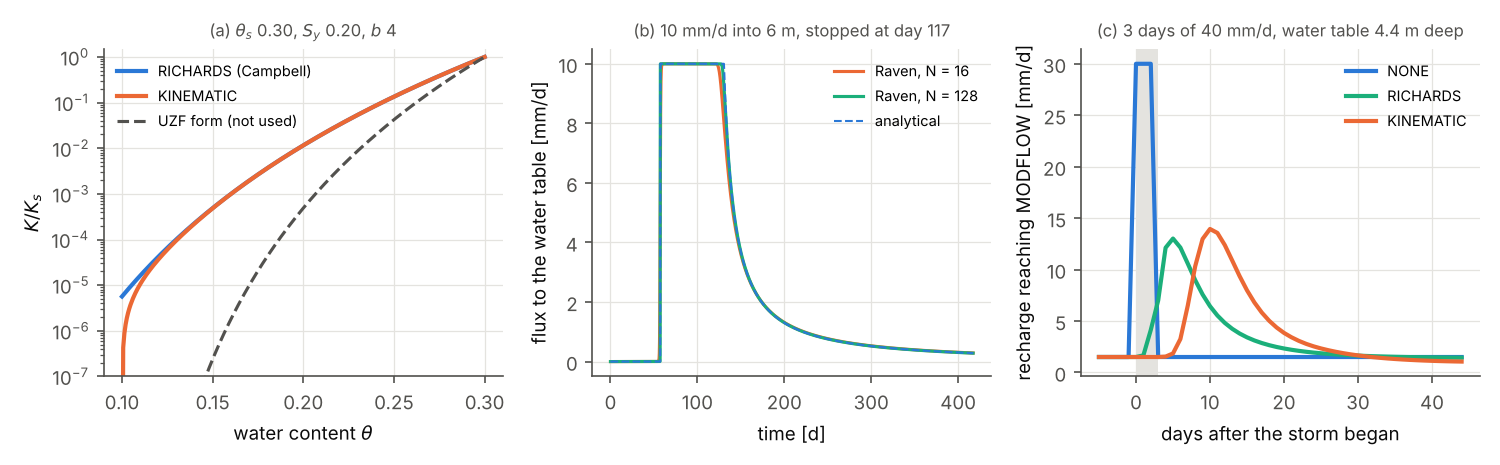
\includegraphics[width=\textwidth]{figures/fig_vz_kinematic.png}
\caption{\cmd{:SoilZoneVadose KINEMATIC}. (a) Conductivity (\ref{eq:kwK}) against Campbell's curve of \cmd{RICHARDS}
and the UZF form. (b) Test K1: flux into the water table of a 6~m column (sand, $K_s$ 0.5~m/d) under 10~mm/d from day 0
to 117, against the analytical kinematic wave (shock, then rarefaction). (c) Test K2: a 3-day storm of 40~mm/d after 400
days of 2~mm/d over a water table 4.4~m below the soil-zone base.}\label{fig:vzkinematic}
\end{figure}

\paragraph{Verification} (\cmd{test\_vz\_kinematic.py}, Section~\ref{ch:verification}).
K1, unit tests (167 checks): over 16\,000 random steps (materials, layers, fluxes, step lengths, \cmd{SPEC\_YIELD} 0) the
balance closes to $10^{-12}$ relative and every content stays within $[\theta_r,\theta_s]$. Against the analytical wave of
Figure~\ref{fig:vzkinematic}b (arrival on day 57.21) the flux reaches half its value on day 57.23 with 16 nodes and 57.21 with
128; the largest error of the drainage tail falls from 5.2\% of $q$ (16 nodes) through 2.7, 1.3 to 0.7\% (128 nodes); with
the default grid, accuracy and daily steps the arrival is 0.5\% late.
K2, the P1 storm: with the columns wetted by 400 days of 2~mm/d, the centroid of the storm's recharge reaches MODFLOW
7.6~days later with \cmd{RICHARDS} and 11.9~days later with \cmd{KINEMATIC}, at a similar peak (921 and 995~m$^3$/d
against 2\,280 without a column; Figure~\ref{fig:vzkinematic}c): without capillarity the front stays sharp and the
mobile water starts lower. Started at rest, as in test P1, the kinematic columns start at $\theta_r$ and soak up the
storm (centroid 72 days later, 15\% of it delivered in 90 days), whereas the Richards columns start at the wetter
hydrostatic profile (9.6 days).
K3 to K6: a water table rising through the column into the soil zone and falling again (the column goes and re-forms),
sand over clay with the water table rising through both, a hotstart continuity check and an existing-model round trip
(flows within $3\times10^{-5}$ of the generated model's); every balance at the standard limits, the column identity of
\cmd{sz\_check} from the first step. K9: the same outputs with a column leak of $10^{-5}$ or $10^{-4}$~m$^3$ per step
written into \cmd{GWBudget.csv} fail these checks.

\paragraph{Cost.} About 3 Newton iterations per node and substep; one 16-node column step costs 7 to 12~$\mu$s against
25 to 30~$\mu$s for \cmd{RICHARDS} on the same machine (unit test K1, timings machine-dependent).

\paragraph{Limits.} No capillarity: no upward redistribution inside the column, no capillary fringe above the water
table, and a sharp wetting front (the real one is smoother). The drained start $\theta_r$ is drier than a real
unsaturated zone: without \cmd{:SoilZoneVadoseInitialFlux} the first recharge of a run wets the columns before any of it
arrives (a few hundred days of 2~mm/d over a few metres). The reference makes the column consistent with MODFLOW's
$S_y$ by construction; a perched water table above a slow layer appears as saturated nodes that back up, not as a
pressure head.

\begin{refcard}{\cmd{:SoilZoneVadose KINEMATIC}}
\cmd{:SoilZoneVadose KINEMATIC} [$\epsilon$ [$N$]] in the \cmd{.rvg} file, with \cmd{:SoilZone PHYSICAL}.
$\epsilon$: largest content change in a substep, (0, 0.2], default 0.02; $N$: nodes per column at most, 3 to 200,
default 16. Materials per MODFLOW layer: \cmd{K\_VERT}, \cmd{POROSITY} ($\theta_s>0$, $\ge$ \cmd{SPEC\_YIELD}),
\cmd{SPEC\_YIELD}, \cmd{CLAPP\_B} (existing models: the model's K33/K and SY, retention of
\cmd{:SoilZoneAquiferClass}). Reference $\theta_s-S_y$; capillary rise from the water table (on by default,
\cmd{:SoilZoneCapillaryRise}); hotstart \cmd{:GWVadoseColumns}.
\end{refcard}

\subsection{A linear storage cascade instead of Richards' equation (LAG)}\label{sec:szvadoselag}
Where only the delay and spreading of recharge through the unsaturated zone matter, \cmd{:SoilZoneVadose LAG} replaces
Richards' equation by a linear storage cascade on the same column: the same nodes, contents, equilibrium profile,
water-table following and hotstart (\cmd{:GWVadoseColumns}) as \cmd{RICHARDS} (Section~\ref{sec:szvadose}); only the
step differs. The water node $i$ holds above its equilibrium content,
\begin{equation}
S_i=(\theta_i-\theta_{\mathrm{eq},i})\,\Delta z_i,\qquad \frac{dS_i}{dt}=Q_{i-1}-Q_i,\qquad Q_i=\frac{\max(S_i,0)}{k_i},\qquad k_i=t_m\,\Delta z_i,
\end{equation}
is the store of a linear reservoir with residence time $k_i$; $Q_0=q_{\mathrm{top}}$ is the column's inflow and $Q_N$ the
flux into the water table, which replaces the column's share of the recharge in \cmd{RCH\_RAVEN}. $t_m$ [d/m] is the travel
time per metre of the node's material, so the mean travel time through a column of one material is $\sum_ik_i=t_mL$ (a
linear kinematic wave of celerity $1/t_m$, discretized as a cascade). Each node uses its own material's $t_m$, so a
column crossing sloping layers of different aquifer classes is a cascade of different residence times.

\paragraph{Travel time.} \cmd{:SoilZoneVadose LAG} $t_m$ gives $t_m$ for every material. Without it (or with 0) $t_m$
is derived per material from the celerity of a kinematic wave at a reference flux $q_r=1$~mm/d, with the conductivity
$K=K_sS_e^{\varepsilon}$, $S_e=(\theta-\theta_s+S_y)/S_y$, $\varepsilon=2b+3$ (Campbell's exponent):
$c=dK/d\theta=\varepsilon q/(S_yS_{e,r})$ at $K=q$, and
\begin{equation}\label{eq:lagtm}
t_m=\frac1c=\frac{S_y\,S_{e,r}}{\varepsilon\,q},\qquad S_{e,r}=\Big(\frac{q}{K_s}\Big)^{1/\varepsilon},\qquad q=\min(q_r,K_s).
\end{equation}
A material with $K_s<q_r$ cannot carry the reference flux: then $q=K_s$, $S_{e,r}=1$ and $t_m=S_y/(\varepsilon K_s)$. $K_s$ =
\cmd{K\_VERT}, $S_y$ = \cmd{SPEC\_YIELD}, $b$ = \cmd{CLAPP\_B} of the aquifer class (for an existing model: the model's
\cmd{K33}/\cmd{K} and \cmd{SY}, and \cmd{CLAPP\_B} of \cmd{:SoilZoneAquiferClass}). The derived value is a starting point;
the travel time is the method's one calibration parameter.

\begin{example}[: derived travel times]
Sand ($K_s=5$~m/d, $S_y=0.25$, $b=4$, $\varepsilon=11$): $S_{e,r}=(0.001/5)^{1/11}=0.461$, $t_m=0.25\times0.461/(11\times0.001)=10.5$~d/m.
Loam ($K_s=0.25$~m/d, $S_y=0.15$, $b=5.4$, $\varepsilon=13.8$): $S_{e,r}=0.670$, $t_m=7.3$~d/m.
Clay ($K_s=2\times10^{-4}$~m/d $<q_r$, $S_y=0.05$, $b=11$, $\varepsilon=25$): $t_m=0.05/(25\times2\times10^{-4})=10.0$~d/m.
A 5~m unsaturated zone in the sand delays recharge by about 52 days on average. The three are similar because a
large $S_y$ (much water to move) offsets a large $K_s$ at the same small flux; at a larger flux the wave is faster
(here the derivation fixes $q_r$). These values are unit test LU of \cmd{test\_vz\_lag.py}.
\end{example}

\paragraph{Spreading.} The spread of the response is set by the node count: its variance is $\sum_ik_i^2$, so the
cascade spreads like $N_{\mathrm{eff}}=(\sum_i k_i)^2/\sum_i k_i^2$ equal reservoirs (for equal ones the response is the
Erlang (gamma) density), with a relative spread $1/\sqrt{N_{\mathrm{eff}}}$. The grid is that of the Richards column (thin
nodes at both ends, growing by 1.3 towards the middle up to $1.3^8$ times the end nodes, $\lceil L/0.05\text{ m}\rceil$
nodes but at least 3 and at most $N$), so $N_{\mathrm{eff}}<N$; beyond 18 nodes the extra ones are of equal thickness and
$N_{\mathrm{eff}}$ grows as about $N-7$. For a column of one material
\begin{center}\small
\begin{tabular}{lcccccccccc}\toprule\hdr
nodes $N$ & 3 & 4 & 6 & 8 & 12 & 16 & 24 & 32 & 50 & 100\\\midrule
$N_{\mathrm{eff}}$ & 2.95 & 3.93 & 5.74 & 7.38 & 10.1 & 12.0 & 17.7 & 25.3 & 43.1 & 93.0\\\bottomrule
\end{tabular}\end{center}
The node count therefore sets the spreading, from a broad response ($N=3$, spread 58\% of the mean) through 29\% for
the default 16 nodes to 15\% for 50 and 10\% for 100; columns shorter than $N\times5$~cm have fewer nodes (at least 3)
(Figure~\ref{fig:vzlagcascade}, left).

\paragraph{The step.} Each Raven step is divided into $n$ equal substeps no longer than the shortest residence time,
$n=\min\big(\max(\lceil\dt/\min_ik_i\rceil,1),50\big)$ (computed in floating point and clamped before it is made an
integer, so that a tiny residence time, with 200 nodes or \cmd{LAG 1e-6}, cannot overflow it). In
each substep every node, top down, is solved exactly with the constant inflow its upper neighbour released in that
substep,
\begin{equation}
S_i(t+h)=S_i(t)\,e^{-h/k_i}+I_ik_i\big(1-e^{-h/k_i}\big),\qquad \text{outflow } S_i(t)+I_ih-S_i(t+h),
\end{equation}
so the nodes pass on exactly what they release and the column conserves water to round-off; $q_{\mathrm{bot}}$ is taken
from the storage change as for \cmd{RICHARDS}. The piecewise-constant transfer between nodes is the only approximation:
against the exact cascade the cumulative response of the default 16-node column differs by at most 1.1\% of the
impulse with daily steps, and the mean travel time by 0.4\%.
A node may not hold more than its porosity, $S_i\le S_{\max,i}=(\theta_s-\theta_{\mathrm{eq},i})\Delta z_i$: water beyond
it passes on to the next node within the substep, and from the last node into the water table. In the capillary
fringe, where $\theta_{\mathrm{eq}}$ is close to $\theta_s$, nodes have almost no room and water crosses it at once; a
large inflow fills the top nodes to saturation and advances as a front at $q/(\theta_s-\theta_{\mathrm{eq}})$, the speed
of a sharp front. A column therefore takes any inflow: nothing is rejected at its top (the soil zone's percolation and
the saturated fraction limit what reaches it); an upward demand ($q_{\mathrm{top}}<0$) is rejected entirely, since
capillary rise into the soil zone comes from the water table through the column by the steady formula
(Section~\ref{sec:szcaprise}), even where a column is active; and an inactive column rejects its inflow and returns
nothing (the contract shared by all methods). A node below equilibrium ($S_i<0$) does not drain; inflow first fills
it. That state arises only from a hotstart written by \cmd{RICHARDS}, the other method with the hydrostatic reference
(\cmd{:GWVadoseColumns RICHARDS}: contents below equilibrium after evaporation or capillary rise): a moving water table remaps the excess and the
equilibrium together, and the cascade itself never takes a node below equilibrium.

\paragraph{Steady start.} With \cmd{:SoilZoneVadoseInitialFlux} $q$ the cascade starts at its steady state for the flux
it receives, $(1-F)\,q$ (Section~\ref{sec:szvadose}; here written $q$),
$S_i=\min(q\,k_i,\,S_{\max,i})$ (a full node passes everything it receives), which delivers $q$ from the first step (unit
test U: to round-off).

\paragraph{Behaviour to expect.} With three depth classes (\cmd{:SoilZoneVadoseClasses 3}) the water table can be lower
during rain than with one class: the upper classes' columns are long (5 to 13~m in the rough-terrain case RT20) and hold
more of the rain in transit. That is the method's own physics, not an error. The cascade has no conductivity limit: a
full column passes any inflow, however slowly permeable its material; where the permeability limits recharge, use
\cmd{RICHARDS} or \cmd{KINEMATIC}.

\begin{example}[: the storm of P1 with LAG]
A 3-day storm of 40~mm/d over a water table 6~m deep, sand with $K_s=0.5$ m/d, $S_y=0.2$, $b=4$ (test L1 of
\cmd{test\_vz\_lag.py}; the case of P1). Without a column the recharge's centroid is on day~6.1; with \cmd{RICHARDS} on
day~15.6. The soil's percolation of the first days (50~mm/d) and the storm pass the capillary fringe (0.3~m) at once and the
storm fills the top nodes. With \cmd{LAG 2} the centroid is on day~13.9 and the peak 30\% below the no-column run, with
\cmd{LAG 4} on day~21.1, and with the derived travel time ($t_m=10.3$~d/m) on day~40.9: delays of 8 to 35 days set by
$t_m$ (Figure~\ref{fig:vzlagcascade}, right). Every identity holds to round-off (largest $4\times10^{-10}$).
\end{example}

\begin{figure}[!htbp]\centering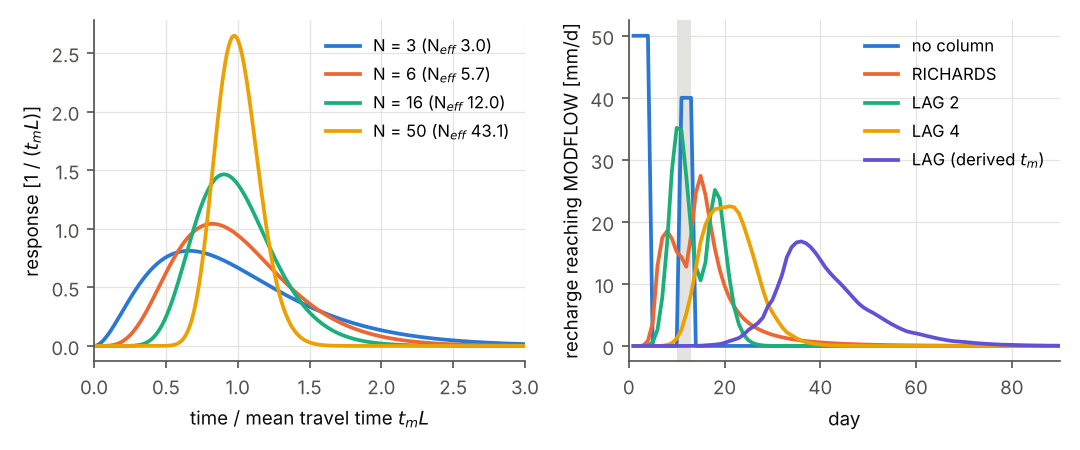
\includegraphics[width=\linewidth]{figures/fig_vz_lag_cascade.png}
\caption{Left: response of a column of one material to an impulse of water at its top, for 3 to 50 nodes on the
column grid (exact cascade; time in units of the mean travel time $t_mL$). Right: recharge reaching MODFLOW in test L1
(3-day storm, grey, over a 6~m unsaturated zone, after four days of percolation from the initial soil water): without a
column, with \cmd{RICHARDS}, and with \cmd{LAG} 2, 4 and the derived travel time.}\label{fig:vzlagcascade}
\end{figure}

\paragraph{Cost and limits.} A column step costs 1 to 3~$\mu$s for 16 nodes (unit test U: 1.7 to 2~$\mu$s), against
12 to 15~$\mu$s for \cmd{RICHARDS}; in a coupled run the water-table following, which remaps the nodes every step (as for
\cmd{RICHARDS}), and the interface iteration cost as much again (test S: 400 columns over a year add 1.4~s to a 1.7~s
run, \cmd{RICHARDS} 2.3~s). The spreading narrows only as $1/\sqrt{N-7}$ with more nodes (each costs time). The cascade
knows no suction: it neither holds water against gravity nor lets the column dry, and its delay does not depend on the
flux (only on $t_m$): a wet year travels as fast as a dry one.

\begin{refcard}{LAG unsaturated columns}
\textbf{Sources/sinks.} Between the soil-zone base and the water table of every exchange column: inflow the column's
unsaturated share of the recharge, outflow to MODFLOW's recharge (\cmd{RCH\_RAVEN}).\par\smallskip
\textbf{Constraints/notes.} Linear reservoirs $k_i=t_m\Delta z_i$ on the Richards grid and its equilibrium profile; mass
conserved to round-off; no content above $\theta_s$; nothing rejected at the top of an active column; capillary rise from
the water table (steady formula); saved in \cmd{solution.rvc} (\cmd{:GWVadoseColumns LAG}), interchangeable with
\cmd{RICHARDS} hotstarts (the same reference profile); a \cmd{KINEMATIC} hotstart's columns start at rest, their water
reported as dropped.\par\smallskip
\par\noindent\begin{minipage}{\linewidth}\textbf{Command syntax}
\begin{lstlisting}
# .rvg
:SoilZoneVadose LAG          # derived travel time per material (q_r = 1 mm/d), 16 nodes at most
:SoilZoneVadose LAG 4 8      # t_m = 4 d/m for every material, 8 nodes at most (3 to 200)
:SoilZoneVadose LAG 0 24     # derived travel time, 24 nodes (N_eff about 18)
\end{lstlisting}
\end{minipage}\par\smallskip
\par\noindent\begin{minipage}{\linewidth}\textbf{Parameters}\par\smallskip
\begin{tabular}{>{\raggedright\arraybackslash}P{0.09\linewidth}>{\raggedright\arraybackslash}P{0.26\linewidth}>{\raggedright\arraybackslash}P{0.283\linewidth}>{\raggedright\arraybackslash}P{0.1\linewidth}>{\raggedright\arraybackslash}P{0.15\linewidth}}\toprule\hdr Symbol & Parameter & Class (where it is set) & Units & Reference\\\midrule
$t_m$ & travel time per metre & \cmd{:SoilZoneVadose LAG} (0: Eq.~\eqref{eq:lagtm}) & d/m & Sec.~\ref{sec:szvadoselag}\\
$N$ & nodes at most & \cmd{:SoilZoneVadose LAG} & -- & Sec.~\ref{sec:szvadose}\\
$K_s$, $S_y$, $b$ & \cmd{K\_VERT}, \cmd{SPEC\_YIELD}, \cmd{CLAPP\_B} & aquifer class (\cmd{:AquiferClasses}) & m/d, --, -- & Sec.~\ref{app:class}\\
$\theta_s$, $\psi_a$ & \cmd{POROSITY}, \cmd{AIR\_ENTRY\_PRESSURE} & aquifer class (equilibrium profile, room) & --, m & Sec.~\ref{app:class}\\
\bottomrule\end{tabular}\end{minipage}\par\smallskip
\textbf{Outputs.} \cmd{GWBudget.csv}: \emph{unsaturated zone inflow}, \emph{unsaturated zone to aquifer},
\emph{unsaturated zone storage} (capillary rise to the soil zone 0: the rise comes from the water table);
\cmd{GWModelSummary.txt}: the method and its nodes.
\end{refcard}

\paragraph{Verification.} \cmd{test\_vz\_lag.py}: LU (unit tests: travel times, mass balance to $5\times10^{-16}$ of the
flows and storage over 16\,000 random steps of 400 random columns, no content above $\theta_s$, nodes below
equilibrium, inactive columns, tiny residence times, steady start, Erlang response of equal reservoirs within 0.6\%,
impulse responses of grid columns against the exact cascade within 1.1\%), L1 (above), L2 (a water table rising
through the columns into the soil zone and falling again), L3 (a column across two aquifer classes on a slope), L4
(restart 60 + 60 days against 120 days: $2\times10^{-8}$), L5 (existing-model round trip: $2.4\times10^{-4}$), L6 (a water table rising into a nearly full top cell releases at
most the room the cell has left), L7 (a column leak of $10^{-5}$ or $10^{-4}$~m$^3$ per step written into a run's
\cmd{GWBudget.csv} fails the script's checks: every run is checked with the column identity of \cmd{sz\_check} from
the first step), LS (cost) and LB
(\cmd{NONE}, \cmd{RICHARDS} and \cmd{CONCEPTUAL} runs byte-identical to a reference build, \cmd{RAVEN\_EXE\_REF}).

\subsection{Depth classes of the unsaturated columns}\label{sec:vzclasses}
The soil zone sees the land of a cell at its $N$ DEM samples (Section~\ref{sec:szslope}), but by default each exchange
column has one unsaturated column, starting at the cell's mean soil-zone base. On irregular ground that is a poor
summary: hummocks have a long unsaturated path and hollows a short one; where the mean base lies within $L_{\min}$ of the
water table there is no column at all, and the hummocks' recharge reaches MODFLOW in the step; where the mean base is
far above the water table, the recharge of hollows that are nearly at the water table is delayed as if they were not.
With \cmd{:SoilZoneVadoseClasses} $K$ ($1\le K\le10$, default 1) every exchange column gets up to $K$ unsaturated
columns, one per \emph{depth class} of its DEM samples, for every method (\cmd{RICHARDS}, \cmd{KINEMATIC}, \cmd{LAG}).

\paragraph{Classes.} The samples' soil-zone bases $z_{b,s}$ (ascending) are grouped into at most $K$ contiguous classes
with the least spread: the grouping minimises $\sum_c\sum_{s\in c}(z_{b,s}-\bar z_c)^2$ (Fisher's optimal partition,
found by dynamic programming over the sorted bases). Unlike groups of equal counts it separates real levels, such as
terraces or pits, from the slopes around them. Equal bases are never split, so $K$ is also limited by the number of
distinct bases (with \cmd{:SoilZoneSubgrid 1} or no DEM there is one class). Class $c$ covers the share $a_c=n_c/N$ of
the column; its unsaturated column starts at $z_b+\bar z_c-\bar z$, the class mean shifted with the column's mean base
$z_b$, so the area-weighted mean of the class tops is $z_b$ (the mean depth to the water table is kept) and $K=1$ is the
single column. Its saturated fraction $F_c(h)=\frac1{n_c}\sum_{s\in c}\sigma((h-z_{b,s})/d_s)$ is the column's $F$ (Section~\ref{ch:soilzone}) on the class's own samples, so
$\sum_c a_c F_c=F$ (to round-off; Raven reports the largest deviation in \cmd{GWModelSummary.txt}). The classes are
fixed for the run.

\paragraph{Water.} Class $c$ takes the unsaturated share $a_c(1-F_{0,c})$ of the column's recharge ($F_{0,c}$ at the
start of the step); a class whose column does not exist (its top within $L_{\min}$ of the water table, or below it)
passes its unsaturated share $a_c(1-F_c)$ to the water table in the step and rejects $a_c F_c$, with its fraction at the
connection head (as a column without unsaturated column). Each class column follows the water table as the single
column does (Section~\ref{sec:szvadose}); the limits of the cell that supplies water to a column (its new nodes, a deficit
below a risen water table, upflow) belong to the soil-zone column, so its classes share them: they are processed in
turn and each has what the earlier ones left; the room of the soil-zone layers for capillary rise is shared likewise.
With \cmd{RICHARDS} each class column gives capillary rise from its top node on its unsaturated share; where a class has
no column (and for \cmd{KINEMATIC} and \cmd{LAG} everywhere) the rise comes from the water table to the class's own base.
That rise takes what the source cell's limit (Section~\ref{sec:szvadose}) has left after all the class columns' draws on
it: the water their new nodes took, the negative recharge passed through them and their bottom upflow; one cell never
gives more than that one limit per step (test C11).
The budget columns of the unsaturated zone (inflow, to aquifer, capillary rise, storage) sum all class columns over
their areas $a\,a_c$, and the identities of Chapter~\ref{ch:balance} hold for them as for one column.

\paragraph{Restart.} With $K>1$ the columns are saved in \cmd{solution.rvc} as \cmd{:GWVadoseClassColumns} (HRU ID, cell,
class, classes of the cell, water table, contents; Appendix~\ref{app:hotstart}). A hotstart written with another $K$
(or another node count) does not stop the run: the columns that do not match start at rest (their reference profile)
and Raven warns. A class column that was inactive at the end of the run that wrote the file (the water table fell below
its base in the last step) has no line; the restart builds it at rest, as the continuous run does in its next step, and
this is not a mismatch (\cmd{test\_vz\_classes.py} C10).

\paragraph{Verification} (\texttt{tests/soilzone/test\_vz\_classes.py}; Figure~\ref{fig:vzclasses}). C1: with $K=1$
the outputs are byte-identical to a build without depth classes (\cmd{NONE}, and \cmd{RICHARDS} where the water table does
not reach, within a step, ground unsaturated at its start; elsewhere the hand-back of rule (i), Section~\ref{sec:szvadose},
is the only difference), the diagnostic column \emph{interface change} left out. C2: a cell with hummocks of $\pm2.5$~m
whose mean base is 3~cm above the water table: with $K=1$ no water passes through a column; with $K=3$ 949~m$^3$ pass
through the hummocks' columns, their outflow 1.79~d after their inflow, with $K=5$ 5\,558~m$^3$ (0.35~d: more of the
area is in short columns). C3: the recharge to MODFLOW approaches the one with every sub-area modelled by its own column
as $K$ grows: nine random squares per cell ($\pm1$~m, water table 1.3~m deep) against $K=9$ (one class per square; with
$5\times5$ samples one class per square would need $K=25$, beyond the limit of 10): relative error 0.0025, 0.00066,
0.00037, 3.6\,$\times10^{-5}$, 3.3\,$\times10^{-5}$, 2.0\,$\times10^{-5}$ and 1.1\,$\times10^{-6}$ for $K=1,2,3,4,5,6,8$;
two terraces 1.2~m apart: 0.0029 with $K=1$ ($K=2$ exact); squares of $\pm1.4$~m over a water table 3~m deep: 0.14,
0.013, 0.0025 and 0.0004 for $K=1,2,4,6$. C4: capillary rise from four class columns under evaporation; C5: water tables
rising and falling through the class columns of four HRUs (shared limits); C6: a specified-head toe, a dried thin top
layer (\cmd{SZW\_RAVEN}), a restart with $K=3$ (20 + 20 days against 40: largest deviation $1.7\times10^{-8}$) and hotstarts
written with $K=1$ read with $K=3$ and vice versa (warning, no stop); C8: \cmd{KINEMATIC} and \cmd{LAG} with $K=3$. In all
of them MODFLOW's balance closes and the recharge, soil-zone and column identities stay below $10^{-8}$ (C4 and C8 below
$10^{-9}$). C7: the cost grows less than in proportion to $K$ (small test cases: 0.32, 0.49 and 0.48~s for $K=1,3,5$;
timings depend on the machine and its load). C9 runs the rough-terrain regression case R20 (\cmd{band\_e43}, an existing
model whose sub-grid bases lie just above the top cell's bottom, \cmd{LAG}) with three classes through
\cmd{test\_rough\_terrain.py}: it checks the interface's connection head (Section~\ref{ch:soilzone}); the saturated
fraction follows the independent closure on converged steps within R20's limit 0.004 (0.0001; a connection head left above
MODFLOW's head gave 0.51).

\begin{figure}[!htbp]\centering
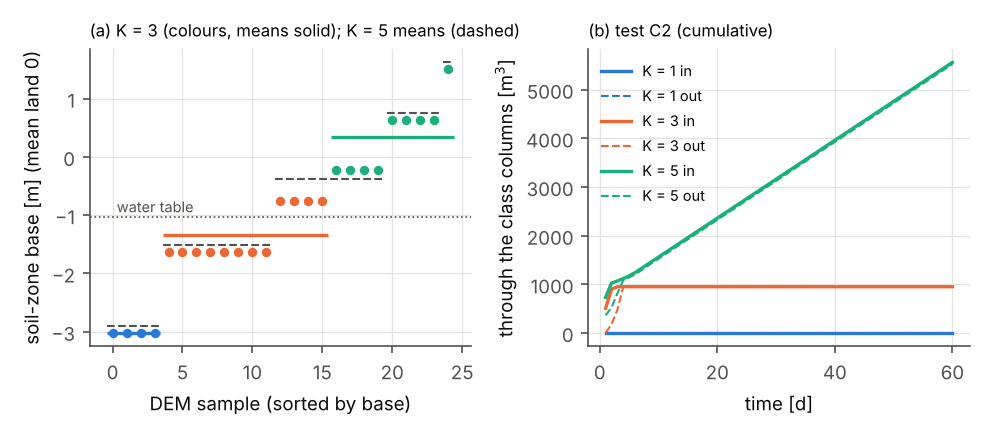
\includegraphics[width=\linewidth]{figures/fig_vz_classes.png}
\caption{Depth classes. (a) The 25 samples of a hummocky cell (test C2), sorted by their soil-zone base, grouped with the least spread
into 3 classes (colours; solid lines: class means) and into 5 (dashed lines: class means, drawn slightly above). (b) Test C2: water entering (solid) and leaving (dashed) the class columns,
cumulative; with $K=1$ the cell has no column.}\label{fig:vzclasses}
\end{figure}

\paragraph{Reference card.} \cmd{:SoilZoneVadoseClasses} $K$ ($1\le K\le10$; default 1: one column per exchange column
at its mean base); classes by least spread of the DEM samples' bases; class $c$: area $a_c$, top at its mean base,
inflow $a_c(1-F_c)$; a class without column passes its share to the water table; limits of the source cell and room of
the soil layers shared by the classes; hotstart \cmd{:GWVadoseClassColumns}.


\subsection{Capillary rise}\label{sec:szcaprise}
Dry soil above a water table draws water up. In a steady upward flux $q$ (positive up) through a profile whose
conductivity depends on the suction $\psi>0$, Darcy's law gives $d\psi/dz=1+q/K(\psi)$, so between two points a height
$\Delta z$ apart, with suctions $\psi_1$ (below) and $\psi_2$ (above),
\begin{equation}\label{eq:rise}
\Delta z=\int_{\psi_1}^{\psi_2}\frac{d\psi}{1+q/K(\psi)},\qquad K(\psi)=\begin{cases}K_s,&\psi\le\psi_a\\K_s(\psi_a/\psi)^m,&\psi>\psi_a\end{cases},\quad m=2+\frac3b .
\end{equation}
The right side falls monotonically from $\psi_2-\psi_1$ ($q=0$) to 0 ($q\to\infty$): there is exactly one $q$ when
$\psi_2-\psi_1>\Delta z$, and none (no rise) when the upper point is at or wetter than hydrostatic. Raven solves
(\ref{eq:rise}) for $q$: in dimensionless form ($u=\psi/\psi_a$, $Q=q/K_s$) the integral is tabulated once per
Clapp--Hornberger exponent, and the root is found with Brent's method on the table (within 2\% of the direct solution
everywhere, mostly within 0.5\%; suctions within a factor $e^2$ of each other are integrated directly). With an
infinitely dry top and a deep water table (\ref{eq:rise}) tends to Gardner's classic result
\cite{gardner1958,eagleson1978}, $q_\infty=K_s\big(1+\tfrac{1.5}{m-1}\big)(\psi_a/d)^m$, which overestimates the rise by
up to 70\% when the soil is only moderately dry (Figure~\ref{fig:szrise}); Raven uses the exact relation.

\paragraph{From the water table.} Where a column has no unsaturated column (no \cmd{:SoilZoneVadose}, or the water
table within $L_{\min}$ of the base or above it), every soil-zone layer $m$ below field capacity whose middle lies above
the water table receives
\begin{gather}
Q_m=\min\Big(A_{k,i}(1-F)\,q\big(\Delta z=z_{\mathrm{mid},m}-h,\ \psi_1=0,\ \psi_2=\psi_{s,m}\big),\ \frac{(\phi_{\mathrm{fc},m}-\phi_m)A_{k,i}}{1000\,\dt}\Big),\\
\psi_{s,m}=\psi_{a,m}\Big(\frac{\phi_m}{\phi_{\max,m}}\Big)^{-b_m},\nonumber
\end{gather}
with the layer's own soil (\cmd{CLAPP\_B}, \cmd{AIR\_ENTRY\_PRESSURE} [mm], \cmd{HYDRAUL\_COND} of its soil class); all
layers together at most the rise to the lowest of them with an infinitely dry top, since the water reaching the upper
layers passes through it. The rise is taken from the aquifer as a fixed rate for the step (through \cmd{SZQ\_RAVEN}) and
added to the layers after the exchange; it is reported as \emph{capillary rise from the water table}.

\paragraph{Which cell supplies it.} Upward flows --- this rise, the unsaturated column's upflow and the repayment of
the lagged exchange's debt --- are rates MODFLOW must take out of a cell. While the top cell holds the water table more
than $\max(5\%\text{ of its thickness},\,5\text{ cm})$ above its bottom they come out of it (\cmd{SZQ\_RAVEN}, the
recharge for the column's upflow). When it has dried, they come out of the highest cell below that does, through a WEL
package \cmd{SZW\_RAVEN} with one entry per active cell below each link's top cell, and the rise is computed from that
cell's head and specific yield: a water table below a thin top layer still feeds the soil (with a 0.5~m
top layer the rise equals that of a thick top layer). When no cell holds
the water table clear of its bottom, the highest cell with water supplies them, scaled down smoothly to zero as it dries
($s^2(3-2s)$ of its saturated part over the margin), so nothing switches on or off abruptly. Out of an aquifer cell they
are moreover together at most half the water it holds above its bottom under the link, faded out the same way,
$\tfrac12 f\,S_yA_{k,i}(h-z_{\mathrm{bot}})/\dt$ per step, so a thin cell is never pumped dry within a step (MODFLOW's solve
can diverge otherwise); the water the new nodes of an unsaturated column take when the water table falls
(below) counts first, then the column's upflow, the rise from the water table and the repayment of the lagged
exchange's debt (what the cell cannot give is repaid later; the column's draw counts also when it goes through the top
cell's recharge); what the column's
upflow does not get from MODFLOW is taken back out of the column, bottom node first, down to air-dry. A specified head
below a dried top cell supplies the rise and the column's upflow itself, without drawdown or limit; MODFLOW ignores a
well in such a cell, so these flows are booked as \emph{specified heads to soil zone} and (the column's) as negative
\emph{recharge onto CHD cells}.

\paragraph{Implicit in the drawdown.} The rise lowers the water table it comes from, and the rate falls steeply with the
depth. A rate from the head at the start of the step overshoots: on dry, conductive soil 5~cm above the water table it
drew 0.1~m in one day and lowered the water table by 0.67~m, which then swung back and forth from step to step. Raven
therefore takes the rate at the end-of-step water table of the column itself,
\begin{equation}\label{eq:riseimpl}
Q=T\Big(\frac{Q\,\dt}{S_y\,A_{k,i}(1-F)}\Big),\qquad T(D)=\min\Big(\sum_m Q_m(\Delta z_m+D),\ Q_{\infty}(\Delta z_{\mathrm{low}}+D)\Big),
\end{equation}
the total rate with the water table lowered by the risen volume over the specific yield and the share's area (no
lateral resupply: the bound of a single column, stable for any step length; $S_y$ at least 0.01). $T$ falls with $D$,
so (\ref{eq:riseimpl}) has one root between $T(T_0w)$ and $T_0$, $w=\dt/(S_yA_{k,i}(1-F))$; Raven finds it with the
Illinois variant of regula falsi (a geometric bisection after a step that does not halve the bracket), keeping the best
lower bound ($T(Qw)$ for every trial $Q$ above the root), to 0.2\% of the root --- about four evaluations of $T$ ---
and the layers keep their shares of $T$. Over specified heads the head does not move and $D=0$. $Q_\infty$ is the rise to
the lowest layer whose middle lies above the water table, whether or not that layer takes water itself, since all rising
water passes through it. With unsaturated columns (any \cmd{:SoilZoneVadose} method) and no column (the water table less than $L_{\min}$ below
the base) the water also crosses the aquifer material between the water table and the base first: $Q_\infty$ is at most
that material's own rise to an infinitely dry top over the gap (\cmd{K\_VERT}, \cmd{CLAPP\_B}, \cmd{AIR\_ENTRY\_PRESSURE}
of the aquifer class), as a column just longer than $L_{\min}$ sees it, so the rise does not jump where the column
appears.

\paragraph{From an unsaturated column.} The same layers receive (\ref{eq:rise}) from the column's top node (its suction
$\psi_1$, the distance from the node to each layer's middle), on the unsaturated share $A_{k,i}(1-F)$ and within the layers'
deficits, and the column's top flux is reduced by the same amount (\emph{capillary rise to soil zone}). In one step the
column passes on at most the larger of the water its top node holds down to the suction of the lowest layer above it
and what the water table itself could supply by (\ref{eq:riseimpl}); what the column cannot deliver within the step
comes back as an unmet upward demand and is not added to the soil. As the column shortens towards $L_{\min}$ its top
node empties and the second term takes over, so the rise just above $L_{\min}$ equals the rise from the water table
just below it (test P9: 1\,732 against 1\,765~m$^3$ on the first day). \cmd{:SoilZoneCapillaryRise ON|OFF} switches both; the default is on with an unsaturated column
(\cmd{:SoilZoneVadose RICHARDS}, \cmd{KINEMATIC} or \cmd{LAG}) and off without one (\cmd{NONE}). \cmd{KINEMATIC} and \cmd{LAG}
columns have no capillarity of their own: with them the rise always comes from the water table (Sections~\ref{sec:szvadosekw}
and~\ref{sec:szvadoselag}).

\begin{example}[: a drying soil over a shallow water table]
Soil zone of 2$\times$0.5~m, $b=5$, $\psi_a=200$~mm, $K_{\mathrm{sat}}=200$~mm/d, PET 4 mm/d and no rain for 60 days
(test P2). Without capillary rise the soil dries in five days and evaporation stops at 15~mm. With it, evaporation
continues on water drawn from the aquifer: 180~mm with the water table 0.7~m deep, 114~mm at 1.3~m and 50~mm at 2.5~m
(Figure~\ref{fig:szcaprise}).
\end{example}

% The soil-zone interface iteration in detail, negative recharge and the MODFLOW side
\subsection{The interface iteration in detail}\label{sec:szinterface}

\paragraph{Schedule.} After each of the first $n_{\mathrm{early}}=\min(5,\max(1,n_{\max}/5))$ outer iterations the interface
is updated whether or not MODFLOW has converged ($n_{\max}$ the outer-iteration limit, \cmd{:SolverMaxOuterIterations} or the
existing model's \cmd{OUTER\_MAXIMUM}); later only after outer iterations on which MODFLOW has converged, at most
\cmd{:SoilZoneIteration} \emph{max} of them. The last tenth of the limit (at least two outer iterations) is left to MODFLOW
on the boundary it has: the update after iteration $n_{\max}-\max(2,n_{\max}/10)$ and the last one the budget allows are
\emph{supply-limited} (below), and once the interface is frozen nothing changes. A step without any update is reported
unconverged. \cmd{:SoilZoneIteration 0} is explicit coupling (the predictor only), and so is an outer-iteration limit of 1,
which leaves no update; both report the interface converged. With a limit of 2 or 3 the step has a single update, whose
flow test compares with the predictor's total exchange.

\paragraph{The rejected recharge as a head-dependent term.} With the connection head $h_c$ of the update MODFLOW receives
the link's recharge $R_l\,(1-F(h_c))$ as a rate and, combined with the exchange's line, the linearization of the rejection
about $h_c$,
\begin{equation}
q_{\mathrm{rej}}(h)=s\,(h_c-h),\qquad s=\max\Big(R_lF'(h_c),\ \frac{R_l\big(F(h^*)-F(h_c)\big)}{h^*-h_c}\Big)\ge0,
\end{equation}
$h^*$ the head MODFLOW returned last (a GHB of head $h_c$ and conductance $s$, merged with the exchange's GHB). MODFLOW's own
iteration then sees that more recharge is rejected as its head rises (over a top layer with $K_v<0.01$~m/d, confined above
its top, the recharge is otherwise a valve of very high gain; with the term the interface of test S1 converges in 4 to 6 outer
iterations per step). The term is booked with the exchange, so mass is exact. On a link
whose unsaturated column carries the step the saturated share is rejected with the fraction of the start of the step $F_0$;
the water the column gives back to the soil zone on ground that saturated since then (rule (i)) follows the connection head
and is in the term, $R_q\min(\max(F(h)-F_0,0),1-F_0)$ with $R_q$ the column's outputs over $1-F_0$ (everything when $F_0=1$;
in explicit coupling only that).

\paragraph{The kink drain.} Where water rises into a soil zone without free water, nothing rises below the level where the
contact ends and the column has nothing to give: the exchange has a kink there, across which a line overshoots (it reverses
into flow out of a column that holds none) and the iteration cycles (test S2). MODFLOW then gets the exchange as a drain
(\cmd{SZD\_RAVEN}) ending at the line's zero, at least the cell bottom $+1$~mm (no DEM sample base lies below that level:
bases are clipped there), steepened at that level to carry the local solve's exchange at the head of linearization (at most
the larger of $C_g$ and the link conductance), its onset smoothed over at least 1~mm. A column that holds free water keeps
the line (it drains below the line's zero).

\paragraph{Convergence.} An update is converged when the last change of every column's soil level is below $\epsilon_h$,
the total exchange changed by no more than $\max(\mathrm{tol}_Q\,G,\ \sum F C\max(\epsilon_h,\mathrm{DVCLOSE}))$ and, per link
in head units (over $K=\max(C,S_ya/\Delta t)$): the rejection at MODFLOW's head and at the connection MODFLOW solved with
differ by less than $\epsilon_h$; the boundary MODFLOW solved with (its HCOF and RHS as booked) differs at the current head
from the local solve's exchange plus the change of the rejection by less than $\epsilon_h$, with only two exemptions --- (i) a
line (not a drain) whose local solves' secant through a real head change (more than $\epsilon_h$, the connection held) has the
wrong sign: its exchange part up to $B=\max(10\,\%\ |Q_c|,\ \epsilon_hK)$; (ii) a kink drain within 1~mm of its level: the
part MODFLOW's smoothing of the drain's onset takes; and the connection MODFLOW solved with gives the converged exchange at
the current head (lag below $\epsilon_hC$ beyond $B$). Then two more tests: the boundary MODFLOW solved with takes from no
column more than it holds at the current heads (the \emph{supply test}), and no link's connection head lies further than
$\max(d_s,10\epsilon_h)$ from MODFLOW's head where the saturated fractions differ by more than $10^{-6}$ (the
\emph{connection test}; specified heads and HDRY skipped). A link failing the connection test has its regula falsi bracket
and its last residual dropped, so that its next update is the plain one ($h_c=h$; counted in \cmd{GWModelSummary.txt},
``connection-test drops''). On the first ten unconverged steps \cmd{Raven\_errors.txt} names the step by its end, the last
change of the soil level and its link (HRU and top active cell), the change of the total exchange and its tolerance --- or,
when both were within the tolerances, the test that failed: the shortfall [m$^3$] and the link of the largest, or the
connection head's distance from MODFLOW's head, its link and the saturated fractions at both heads. No update is made from an
iterate MODFLOW has not converged on that holds a head that is not finite, or in which a link's top cell lies far outside the
model's elevations (the divergence margin below) and away from that link's connection head (more than the margin from it,
and on the other side of the model or more than the margin further outside).

\paragraph{Supply limits.} In explicit coupling and on the supply-limited update the boundary MODFLOW keeps may not take more
from a column than its free water, down to the lowest head the cell can reach (the bottom of the column's lowest active
cell): first the rejection's term ($s(h_c-z_{\mathrm{low}})$ at most the head-dependent rejection and at most the free water
the line leaves), then the line with what the term leaves. \cmd{GWModelSummary.txt} reports the number of such link updates
and the largest take beyond the free water (0 up to round-off).

\paragraph{Negative recharge.}\label{sec:negrecharge} A process that takes water out of \cmd{GROUNDWATER} (e.g. \cmd{PERC\_GR4JEXCH SOIL[1]
GROUNDWATER} with a positive \cmd{GR4J\_X2}) gives a negative recharge. On an HRU with a soil zone it is never split by $F$: all
of it is taken from MODFLOW (through the column on a column link), at most what the top cell can still give in the step
(half its water above its bottom under the link, less what the columns, the capillary rise and the repayment of a lagged
debt took before); the rest is cut and taken back out of the soil zone as a negative rejected recharge (run total ``negative
recharge cut''). What the soil zone does not hold of that cut (a process after the import moved it on before the coupled
exchange) is taken from the HRU's other columns in proportion to their water, and only what the whole HRU cannot supply is
booked as ``negative recharge the soil zone did not hold'' (its own \cmd{GWBudget.csv} column, warning and run total). On HRUs
without a soil zone and without \cmd{:SoilZone PHYSICAL} it is plain recharge, not limited (a warning).

\paragraph{Drained columns.}\label{sec:drained} With \cmd{NEWTON}, before each solve a column whose active cells are all convertible
(\cmd{ICELLTYPE}$\neq0$: a generated model's layer types, an existing model's from MODFLOW's memory) and whose lowest cell is
at or below its bottom is set 1~mm above that bottom in MODFLOW's iterate, once per step, once more on a later solve of the
step that leaves the lowest cell more than 1~m below its bottom, and after a solve with heads that are not finite; never in
the last two outer iterations (except for heads that are not finite). A column with an active confined cell is never drained.

\paragraph{Heads far outside the model.} A step whose heads are not finite stops the run at once. A step MODFLOW did not
converge on that holds a head beyond the model's highest top or lowest bottom by more than ten times its relief (at least
1~km) is carried on only if every such head that moved in the step (relative to the heads of the last converged step, by
position) moved by at most that margin in the last outer iteration and MODFLOW's residual is at most 1\,\% of the gross flow
through the aquifer (every entry's inflow and outflow, MODFLOW's TOTAL IN plus TOTAL OUT; Raven's percentage divides by
IN$+$OUT, half MODFLOW's PERCENT DISCREPANCY); such a step is warned with its residual. Otherwise the run stops, naming the
head, its cell, its last move, the residual and the usual causes. An unconverged step without a far head is carried on
whatever its residual, as MODFLOW's own \cmd{CONTINUE} option would: the residual is MODFLOW's balance error and a negative one
is withheld from the discharge returned to Raven. A far head on a converged step is warned about once per run (per ensemble
member).

\paragraph{Existing models.} \cmd{:SoilZone PHYSICAL} needs an existing model with \cmd{NEWTON} (start-up stop naming the name
file; MODFLOW then needs \cmd{LINEAR\_ACCELERATION BICGSTAB}). A model without a storage package is steady state: storage 0,
$S_y$ taken from \cmd{SPEC\_YIELD} of \cmd{:SoilZoneAquiferClass} when that class gives it, otherwise 0.2 (a warning naming
the value either way) for the soil-zone checks, the release limits and the columns; with one, \cmd{SY} is taken as
MODFLOW holds it, also where it is 0 (common with \cmd{ICONVERT} 0, all of the model included), floored at 0.01 for the
release limits and the columns, with a warning counting the cells below 0.01: such a model's outputs are unchanged. The warning
about an outer-iteration limit below 20 is written once MODFLOW's limit is known (\cmd{OUTER\_MAXIMUM} for an existing model).
A restart writes the heads with 17 significant digits and writes 0 as the lagged exchange of links whose cell was a specified
head in the last step. Without \cmd{NEWTON} (\cmd{:SoilZone CONCEPTUAL}) the recharge MODFLOW does not apply to a column whose
cells are all dry or whose highest active cell is a specified head is booked, signed, as ``recharge not applied by MODFLOW''
(the water such cells held when they dried is in neither balance; confined cells never dry).


\subsection{Timing within a step}\label{sec:sztiming}
Raven's processes and the exchange cannot both come first within a step. With \cmd{:SoilZoneExchangeTiming AFTER}
the processes run first and do not see the water the exchange brings in the same step. With \cmd{LAGGED}, the
default, each column first receives its exchange of the last step,
\begin{equation}
L_c=-q_c^{\,n-1}\dt\quad\text{(limited to the column's room or water)},
\end{equation}
so that evaporation and drainage see the water that is rising in; when the exchange of the step begins the source is
taken back out of the column as far as the column still holds it ($r_c$), and what the processes used of it,
$D_c=-L_c-r_c$, is settled after the step's exchange:
\begin{equation}
\Delta\phi_c=L_c+r_c+\big(-q_c^{\,n}\dt+D_c\big)=-q_c^{\,n}\dt .
\end{equation}
Over the step the column receives exactly MODFLOW's booked exchange; only the order changes, and the splitting error
scales with $q^n-q^{n-1}$ instead of $q^n$. If the column cannot give back $D_c$ (the processes used more of the lent
water than the step's exchange supplied), the remainder is a \emph{debt} that the aquifer repays in the following
steps through \cmd{SZQ\_RAVEN}; nothing is created or lost (\emph{lagged-exchange debt}, \emph{lagged-exchange
repayment}). A column that was a specified head in the last step exchanged exactly, so it has no lagged source in the
next step, whether or not its head is held in that step (a \cmd{:BoundaryHead} series can switch it). The last step's
exchange (0 for such a column) and any open debt are saved in \cmd{solution.rvc} (\cmd{:GWSoilZoneLag}), so a restart
continues exactly, also at a switch of the specified heads. On the hillslope test the mean head difference to the MODFLOW-only reference falls from
1.8~cm to 0.7~cm and the largest from 6.6~cm to 2.5~cm, with 20\% fewer outer iterations (Figure~\ref{fig:sztiming}).

\subsection{Raven's processes on each part of an HRU}\label{sec:szclasses}
Raven's processes act on an HRU's state, but the columns of an HRU can be very different: saturated at the foot of a
slope, dry at its top. With \cmd{:SoilZoneClasses} $N_c$ the columns of each HRU are sorted at the start of every step by
their saturated thickness $b^{\mathrm{sz}}$, then their soil water, and grouped into up to $N_c$ classes of about equal area
(classes with the same soil water are merged). In Raven's \cmd{ORDERED\_SERIES} solver the HRU's process sequence then
runs once per class $c$ on a copy of the HRU's state with the class's mean soil water $\bar\phi_c$; the HRU's state
becomes the area-weighted mean $\sum_cw_c\,\phi_c$ of the results (exact for every water store, since each run
conserves water), the balances are weighted alike, and each class's result is shared among its own columns. With as
many classes as columns an HRU behaves exactly like one HRU per cell (test P6: heads within $6.5\times10^{-7}$~m). The cost is $N_c$
evaluations of the HRU's processes per step. Other solvers keep the HRU mean (with a warning).

\subsection{Columns over specified heads}\label{sec:szchd}
Links on cells whose top active layer is a specified head have soil-zone columns too. MODFLOW does not apply
boundaries on specified-head cells, and needs none: the head is known. After MODFLOW's solve each such column is
solved with the specified head $h^{\mathrm{chd}}_i$,
\begin{equation}
\Delta\phi+\frac{1000\,\dt}{A_{k,i}}\,q^{\mathrm{sz}}_{k,i}\big(b^{\mathrm{sz}}(\phi^*+\Delta\phi),h^{\mathrm{chd}}_i\big)=0,
\end{equation}
which is exact for that column (the head does not respond), and the flow is booked as \emph{soil zone to specified
heads} or \emph{specified heads to soil zone}; capillary rise there comes from the head as well. The column's recharge
goes to the specified head (\emph{recharge onto CHD cells}), rejected where the ground is saturated. With an existing
model the specified-head cells may change with its stress periods; the columns follow them step by step. An existing
model's specified heads are known only once MODFLOW has read the step's period (from the first step on), so unsaturated
columns (Section~\ref{sec:szvadose}) can exist on such cells: in a step in which a link's cell is a specified head its
unsaturated columns end, their water above their reference profiles going to the specified head (\emph{recharge onto CHD
cells}; a run total in \cmd{GWModelSummary.txt}), and a column forms again, at rest, when the cell is no longer one. The
rest column of an HRU covers only the part outside the grid, where there is no aquifer to exchange with.

\subsection{With an existing MODFLOW model}\label{sec:szexisting}
\cmd{:SoilZone PHYSICAL} works with \cmd{:MF6Simulation} as with a generated model (Chapter~\ref{ch:existing}). Raven adds
\cmd{raven.szx} (GHB \cmd{SZX\_RAVEN}), \cmd{raven.szq} (WEL \cmd{SZQ\_RAVEN}), \cmd{raven.szd} (DRN \cmd{SZD\_RAVEN})
and, with more than one layer, \cmd{raven.szw} (WEL \cmd{SZW\_RAVEN}, Section~\ref{sec:szcaprise}) to the model's name
file next to \cmd{raven.rch}. The soil zone lies on the model's top: the soil-zone base is the top
of the top active cell and the land surface is $d_{\mathrm{sz},k}$ higher. Its relief within a cell comes from \cmd{:LandSurface}
when given (the DEM's points about their mean in the cell; an \cmd{:OverlapWeights} table has no cell outlines to sample
the DEM in, so each cell is flat and a warning says that \cmd{:LandSurface} is not used). The soil--aquifer conductance and the storage check use the model's own vertical
conductivity (\cmd{K33}, else \cmd{K}) and specific yield of the top active cell; unsaturated columns take the
conductivity and specific yield of every layer from the model, and $b$, $\psi_a$ and $\theta_s$ from
\cmd{:SoilZoneAquiferClass} (Section~\ref{app:commands}). A steady model (no storage package) has no specific yield: the
\cmd{SPEC\_YIELD} of \cmd{:SoilZoneAquiferClass} is used when the class gives it, otherwise 0.2. Heads, conductances and rates are converted from the model's
length and time units. A generated soil-zone model coupled again as an existing model reproduces the generated run
within the interface tolerances, also in feet and seconds (tests X1--X4).
The model must use MODFLOW's \cmd{NEWTON} formulation (Raven stops at start-up otherwise, naming the name file to edit;
MODFLOW then also needs \cmd{LINEAR\_ACCELERATION BICGSTAB}): without it a top cell that dries leaves the solve (head
HDRY), and the recharge, the soil-zone exchange and the columns over it would lose their cell until it rewets (test X6). Raven stops when MODFLOW's heads are not finite, or when a step MODFLOW did not converge leaves a head far outside the
model's elevations (beyond its highest top or lowest bottom by more than ten times its relief, at least 1~km: a diverged
solve), rather than carry them on; the message names the cell and the date. Such a head on a converged step is what
MODFLOW computes from the input (for instance recharge into a confined cell under a dried top cell without
\cmd{NEWTON}) and gives a warning.

\subsection{Cost}\label{sec:szcost}
The unsaturated columns cost about 40~$\mu$s per column and day in a wet spell and much less when nothing moves;
capillary rise costs a few table lookups per column and step (a few more for the drawdown root), the specified-head columns one local solve per column and step; classes
cost $N_c$ evaluations of the HRU's processes. On the Liard example with \cmd{:SoilZone PHYSICAL} (85 HRUs, 4\,286 links,
one year, optimized build) the run takes 69~s with the defaults, and 91~s with unsaturated columns, capillary rise
and three classes (6\,378 outer iterations against 4\,809); MODFLOW's solve remains the larger part.

\begin{refcard}{soil zone}
\textbf{Sources/sinks.} Moves water both ways between the soil-zone columns of each coupled HRU with soil (Raven's
\cmd{SOIL[0..$M-1$]} hold their mean) and the top active cell of each overlapping column (MODFLOW GHB \cmd{SZX\_RAVEN} with WEL
\cmd{SZQ\_RAVEN} and DRN \cmd{SZD\_RAVEN}; upward flows out of the cell holding the water table below a dried top cell
through WEL \cmd{SZW\_RAVEN}); returns rejected recharge to the columns and sends overflow to \cmd{SURFACE\_WATER}.\par\smallskip
\textbf{Constraints/notes.} Recharge must come from \cmd{SOIL[$M-1$]}; every soil-zone layer needs a positive thickness and
drainable porosity, and the class of \cmd{SOIL[$M-1$]} needs \cmd{HYDRAUL\_COND}. \cmd{RECHARGE\_DELAY} must be 0 for
soil-zone HRUs; \cmd{:SoilZoneVadose LAG} (Section~\ref{sec:szvadoselag}) delays recharge through a deep unsaturated zone instead
(only below the soil zone, so recharge on saturated ground is still rejected). Works with an existing model (\cmd{:MF6Simulation}; Section~\ref{sec:szexisting}). With the default
\cmd{LAGGED} timing the splitting error of Raven's processes ahead of the exchange scales with the change of the
exchange between steps (hillslope test: 0.7 cm mean head difference at daily steps; 1.8 cm with \cmd{AFTER}).
Capillary rise needs \cmd{CLAPP\_B} and \cmd{AIR\_ENTRY\_PRESSURE} of the soil classes (Raven estimates them from the
texture otherwise); unsaturated columns need them for the aquifer classes. \cmd{:SoilZoneClasses} needs
\cmd{:Method ORDERED\_SERIES}. Keep $d_s>0$ (below 0.1~m Raven warns). The saturated fraction that rejects recharge is
recomputed on every interface update from MODFLOW's current head, so the rejection follows the converged head of the
step (Section~\ref{sec:szinterface}); only the share of the recharge that an unsaturated column carries through the
step is split with the fraction at the start of the step, $F_0$ (the column's inflow is set before MODFLOW's solve), and
a rise of the fraction during the step hands that share back as rejected recharge. With unsaturated columns give $S_y$ close to the drainable porosity of
the aquifer class (Raven warns otherwise).\par\smallskip
\par\noindent\begin{minipage}{\linewidth}\textbf{Command syntax}
\begin{lstlisting}
# .rvg
:SoilZone PHYSICAL SOIL[0] SOIL[1]      # layers from the top; default CONCEPTUAL
:SoilZoneIteration 100 1.0E-4 1.0E-6    # updates after MODFLOW converged, tolerances
:SoilZoneSubgrid 5                      # DEM points per cell side
:SoilZoneOutput  WetlandHRUs            # optional: GWSoilExchange.csv for one group
:SoilZoneVadose RICHARDS 0.02 16        # unsaturated columns: accuracy, nodes; default NONE
                                        # also KINEMATIC {accuracy} {nodes}, LAG {t_m [d/m]} {nodes}
:SoilZoneVadoseClasses 3                # unsaturated columns per exchange column (depth classes); default 1
:SoilZoneVadoseInitialFlux 2            # steady start of the columns for 2 mm/d; default 0 (at rest)
:SoilZoneCapillaryRise ON               # default ON with RICHARDS/KINEMATIC/LAG, OFF with NONE
:SoilZoneExchangeTiming LAGGED          # default LAGGED; AFTER: after Raven's processes
:SoilZoneClasses 5                      # Raven's processes per class of columns; default 1
:SoilZoneAquiferClass SAND              # existing models: b, psi_a, theta_s of the cells (unsaturated columns)
# .rvi -- recharge from the bottom soil-zone layer
:Percolation PERC_GAWSER SOIL[1] GROUNDWATER
\end{lstlisting}
\end{minipage}\par\smallskip
\par\noindent\begin{minipage}{\linewidth}\textbf{Parameters}\par\smallskip
\begin{tabular}{>{\raggedright\arraybackslash}P{0.09\linewidth}>{\raggedright\arraybackslash}P{0.26\linewidth}>{\raggedright\arraybackslash}P{0.283\linewidth}>{\raggedright\arraybackslash}P{0.1\linewidth}>{\raggedright\arraybackslash}P{0.15\linewidth}}\toprule\hdr Symbol & Parameter & Class (where it is set) & Units & Reference\\\midrule
$H_m$ & layer thickness & soil profile (\cmd{:SoilProfiles}, \cmd{.rvp}) & m & Raven manual\\
$\eta_m$, $S_{\mathrm{fc},m}$, $\mathit{SF}_m$ & \cmd{POROSITY}, \cmd{FIELD\_CAPACITY}, \cmd{STONE\_FRAC} & soil class (\cmd{.rvp}) & -- & Raven manual\\
$K_{\mathrm{sat},M-1}$ & \cmd{HYDRAUL\_COND} & soil class of \cmd{SOIL[$M-1$]} (\cmd{.rvp}) & mm/d & Raven manual\\
$K_v$, $S_y$ & \cmd{K\_VERT}, \cmd{SPEC\_YIELD} & aquifer class of the top layer & m/d, -- & Sec.~\ref{app:class}\\
$d_s$ & \cmd{SEEPAGE\_SMOOTHING\_DEPTH} & aquifer profile & m & Sec.~\ref{app:profile}\\
$b$, $\psi_a$ (soil) & \cmd{CLAPP\_B}, \cmd{AIR\_ENTRY\_PRESSURE} & soil class (\cmd{.rvp}) & --, mm & Raven manual\\
$b$, $\psi_a$, $\theta_s$ & \cmd{CLAPP\_B}, \cmd{AIR\_ENTRY\_PRESSURE}, \cmd{POROSITY} & aquifer class & --, m, -- & Sec.~\ref{app:class}\\
$N_g$ & \cmd{:SoilZoneSubgrid} (points per side, squared) & \cmd{.rvg} & -- & Sec.~\ref{app:commands}\\
\bottomrule\end{tabular}\end{minipage}\par\smallskip
\textbf{Outputs.} \cmd{GWBudget.csv}: \emph{soil zone to aquifer}, \emph{aquifer to soil zone}, \emph{rejected recharge},
\emph{soil-zone overflow}, \emph{soil-zone exchange applied to Raven}, \emph{soil-zone shortfall}, \emph{interface updates},
\emph{interface converged}, \emph{interface change}, \emph{soil-zone layer redistribution}, \emph{seepage and soil inflow withheld}, \emph{river gains withheld}, \emph{surface-store gains withheld};
with unsaturated columns, capillary rise, \cmd{LAGGED} timing or columns over specified heads also \emph{unsaturated zone inflow}, \emph{unsaturated zone to aquifer}, \emph{capillary rise to soil
zone}, \emph{unsaturated zone storage}, \emph{capillary rise from the water table}, \emph{lagged-exchange debt},
\emph{lagged-exchange repayment}, \emph{soil zone to specified heads}, \emph{specified heads to soil zone}
(Section~\ref{sec:accsz}); \cmd{GWSoilExchange.csv} per HRU and step: soil-zone base, soil water
level, water table, saturated fraction, exchange with the aquifer (and with specified heads, where the model has them,
under the headings of \cmd{GWBudget.csv}), rejected recharge, overflow, soil water and capacity.
\cmd{tools/plot\_soilzone.py} plots both, the exchange with specified heads as lines of its own.
\end{refcard}

\subsection{Common questions}
\textit{Which layers should form the soil zone?} Physical soil layers above the aquifer, typically the top one or two;
not conceptual reservoirs of tens of metres (a soil zone over 20 m stops the run, over 5 m gives a warning).
\textit{Does $S_y$ have to match the soil?} No, but where the top aquifer layer's $S_y$ and the soil's drainable porosity
differ by more than a factor two the water table rises at visibly different rates below and inside the soil, and a
warning says so. \textit{Why does an HRU's soil level differ from its cells' water tables?} The HRU value is the mean
over its columns; \cmd{GWSoilExchange.csv} reports area-weighted means. \textit{How short should the step be?} Daily
steps are adequate for most catchments; where the soil zone fills and drains within a day, sub-daily steps reduce the
splitting error. \textit{Do I need the unsaturated columns?} Where the water table is more than a metre or two below
the soil for long periods, yes: without them recharge reaches MODFLOW when it leaves the soil. \textit{How many
classes?} Three to five capture most of the difference between wet and dry parts of an HRU; as many as an HRU has
cells reproduces one HRU per cell.

\section{Rivers}\label{ch:rivers}
Rivers exchange water with the aquifer in both directions: a \emph{gaining} river receives groundwater (baseflow); a
\emph{losing} river leaks into the aquifer. The coupling uses MODFLOW's RIV package in every cell crossed by a river line
(\cmd{:RiverGeometry}), with river levels taken from Raven's own river routing.

\subsection{River cells}
River lines (GeoJSON, lon/lat) are cut into short pieces (1/20 of a cell) and each piece is assigned to the cell under its
midpoint. For each subbasin $p$ and cell $i$ Raven records the river length $L_{p,i}$ and the lowest DEM value along the
line in that cell. The subbasin of a piece comes from an ID field in the GeoJSON, or, if none is given, from the subbasin
of the dominant HRU of the cell.

\subsection{Riverbed elevation and river level}
The DEM usually records the water surface or floodplain along a river, so the bed lies one bankfull depth below it:
\begin{equation}
z_{\mathrm{bed}}=\min_{\text{line in cell}}z_{\mathrm{DEM}}-d_{\mathrm{bf},p},
\end{equation}
where $d_{\mathrm{bf},p}$ is the depth of Raven's channel at its reference flow (or the value of \cmd{:RiverBedDepth});
$z_{\mathrm{bed}}$ is also never placed above the model top.
The bed is never placed above the model top nor below the column: if it would lie below every active cell, it is set
0.1 m above the lowest active cell bottom. The river cell is placed in the highest active layer whose bottom is below the
bed. Each day the river level (\emph{stage}) is
\begin{equation}
s=\min\!\left(z_{\mathrm{bed}}+d_p(t),\ z_{\mathrm{land},i}\right),
\end{equation}
with $d_p(t)$ Raven's channel depth at the start of the day. Above bankfull the extra water is on the floodplain, which
is not part of this exchange, so the stage is capped at the land surface.

\subsection{Exchange equation}
\begin{equation}
q^{\mathrm{riv}}=\begin{cases}C^{\mathrm{riv}}\left(s-h\right) & h>z_{\mathrm{bed}},\\
C^{\mathrm{riv}}\left(s-z_{\mathrm{bed}}\right) & h\le z_{\mathrm{bed}},\end{cases}
\qquad C^{\mathrm{riv}}=\frac{K_b\,W_p(t)\,L_{p,i}}{M_b},
\end{equation}
with $K_b$ [m/d] the riverbed conductivity (aquifer profile parameter \cmd{RIVERBED\_K}), $M_b$ [m] its thickness (aquifer profile parameter \cmd{RIVERBED\_THICKNESS}; Section~\ref{app:profile}) and $W_p(t)$
Raven's channel top width. Positive $q$ is a losing river. When the water table drops below the bed, the river is
\emph{disconnected}: it leaks at a constant maximum rate, whatever the depth of the water table
(Figure~\ref{fig:curves}c).

\begin{figure}[!htbp]\centering
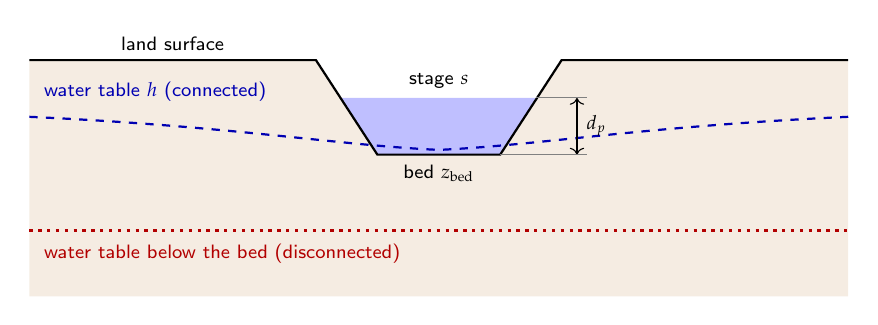
\begin{tikzpicture}[x=1.3cm,y=1.2cm,lab/.style={font=\scriptsize}]
\fill[brown!15] (-4,0) -- (4,0) -- (4,2.5) -- (1.2,2.5) -- (0.6,1.5) -- (-0.6,1.5) -- (-1.2,2.5) -- (-4,2.5) -- cycle;
\fill[blue!25] (-0.95,2.1) -- (0.95,2.1) -- (0.6,1.5) -- (-0.6,1.5) -- cycle;
\draw[thick] (-4,2.5) -- (-1.2,2.5) -- (-0.6,1.5) -- (0.6,1.5) -- (1.2,2.5) -- (4,2.5);
\draw[dashed,blue!70!black,thick] (-4,1.9) .. controls (-2,1.8) and (-1,1.6) .. (0,1.55) .. controls (1,1.6) and (2,1.8) .. (4,1.9);
\node[lab,blue!70!black,anchor=west] at (-3.95,2.17) {water table $h$ (connected)};
\draw[dotted,red!70!black,very thick] (-4,0.7) -- (4,0.7); \node[lab,red!70!black,anchor=west] at (-3.95,0.45) {water table below the bed (disconnected)};
\draw[<->] (1.35,1.5) -- (1.35,2.1); \node[lab,right] at (1.35,1.8) {$d_p$};
\draw[gray,thin] (0.6,1.5) -- (1.45,1.5); \draw[gray,thin] (0.95,2.1) -- (1.45,2.1);
\node[lab] at (0,2.28) {stage $s$}; \node[lab] at (0,1.3) {bed $z_{\mathrm{bed}}$};
\node[lab,anchor=south] at (-2.6,2.5) {land surface};
\end{tikzpicture}
\caption{River cell: stage $s$ = bed + Raven channel depth. With the water table above the bed, flow is $C(s-h)$ (either
direction); below the bed the river is disconnected and leaks at $C(s-z_{\mathrm{bed}})$.}\label{fig:river}
\end{figure}

\subsection{Never taking water the river does not have}
A losing river cannot give more than it carries. The conductance is therefore limited each day so that the largest
possible loss --- the disconnected rate $C(s-z_{\mathrm{bed}})$ --- is no more than the cell's share (by river length) of
the flow in the channel reach at the start of the day (the channel flow, upstream of any reservoir at the subbasin outlet):
\begin{equation}
C^{\mathrm{riv}}\le\frac{86\,400\,Q^{\mathrm{out}}_p\,(L_{p,i}/L_p)}{s-z_{\mathrm{bed}}},
\end{equation}
with $Q^{\mathrm{out}}_p$ in m$^3$/s ($\times86\,400$ gives m$^3$/d) and $L_p$ the subbasin's total river length on active cells. (Using the reservoir
release instead would cut off every river cell above a lake whenever the lake is not spilling.) Rivers of disabled
subbasins get no river cells.

\subsection{Back to Raven's rivers}
For each subbasin the net aquifer discharge is $G_p=-\sum_i q^{\mathrm{riv}}_{p,i}$ [m$^3$/d]. A gain is added to the
subbasin's in-catchment inflow for the day (so it passes Raven's catchment routing like other runoff). A loss is taken
first from that in-catchment inflow and then, inside Raven's routing loop, from the flow entering the reach from
upstream. A loss that still cannot be supplied in the day --- rare, because of the limit above --- is \emph{carried} to the
next day and taken from the river first thing then, so no water is created:
\begin{equation}
V^{\mathrm{applied},n}_p=G^n_p\,\dt-V^{\mathrm{carry},n-1}_p+V^{\mathrm{carry},n}_p,
\end{equation}
where $G^n_p$ is $G_p$ on day $n$ and $V^{\mathrm{carry},n}_p$ [m$^3$] is the loss carried out of day $n$. Summed over a run, the water applied to Raven equals MODFLOW's net
river exchange minus whatever is still carried at the end (written to \cmd{solution.rvc} as \cmd{:GWRiverLossCarry} and
taken on the first day of a restart).
\begin{example}[: river exchange]
$K_b=0.5$ m/d, $M_b=1$ m, width 40 m, 2\,500 m of river in the cell: $C=0.5\times40\times2\,500/1=50\,000$ m$^2$/d. Bed
590 m, depth 1.5 m, stage 591.5 m. Water table at 590.8 m: $q=50\,000\times0.7=35\,000$ m$^3$/d lost to the aquifer.
Water table at 592.0 m: $q=-25\,000$ m$^3$/d, a gain for the river. Water table at 585 m (below the bed): the river
leaks $50\,000\times1.5=75\,000$ m$^3$/d.
\end{example}

\begin{refcard}{rivers}
\textbf{Sources/sinks.} Exchanges water in both directions between the aquifer (MODFLOW RIV package \cmd{RIV\_RAVEN} in every river cell) and Raven's
reaches: gains are added to the subbasin's in-catchment inflow; losses are taken from it and then from the reach inflow.\par\smallskip
\textbf{Constraints/notes.} The conductance is limited by the channel flow at the start of the step; a loss that cannot be supplied is carried to the next
step. The stage never exceeds the land surface; the bed is never above the model top. Disabled subbasins get no river cells.\par\smallskip
\par\noindent\begin{minipage}{\linewidth}\textbf{Command syntax}
\begin{lstlisting}
# .rvg
:RiverGeometry  my_rivers.geojson  SubId     # river lines; subbasin ID field optional
:RiverBedDepth  REFERENCE_FLOW               # or a depth [m] below the DEM
# .rvp
:AquiferProfileParameters
  :Attributes,     RIVERBED_K, RIVERBED_THICKNESS
  :Units,          m/d,        m
  VALLEY_ALLUVIUM, 0.5,        1.0
:EndAquiferProfileParameters
\end{lstlisting}
\end{minipage}\par\smallskip
\par\noindent\begin{minipage}{\linewidth}\textbf{Parameters}\par\smallskip
\begin{tabular}{>{\raggedright\arraybackslash}P{0.09\linewidth}>{\raggedright\arraybackslash}P{0.26\linewidth}>{\raggedright\arraybackslash}P{0.283\linewidth}>{\raggedright\arraybackslash}P{0.1\linewidth}>{\raggedright\arraybackslash}P{0.15\linewidth}}\toprule\hdr \hdr Symbol & Parameter & Class (where it is set) & Units & Reference\\\midrule
$K_b$ & \cmd{RIVERBED\_K} & aquifer profile (of the column) & m/d & Sec.~\ref{app:profile}\\
$M_b$ & \cmd{RIVERBED\_THICKNESS} & aquifer profile & m & Sec.~\ref{app:profile}\\
$W_p$, $d_p$ & channel top width, depth & subbasin channel (\cmd{:ChannelProfile}, \cmd{.rvp}); Raven routing state & m & Raven manual\\
$d_{\mathrm{bf},p}$ & \cmd{:RiverBedDepth} or depth at \cmd{Q\_REFERENCE} & \cmd{.rvg} option; subbasin parameter (\cmd{.rvh}) & m & Sec.~\ref{app:commands}\\
$L_{p,i}$ & river length in a cell & computed from \cmd{:RiverGeometry} & m & Sec.~\ref{ch:rivers}\\
$Q^{\mathrm{out}}_p$ & channel flow & Raven routing state (subbasin) & m$^3$/s & Raven state var.\\
\bottomrule\end{tabular}\end{minipage}\par\smallskip
\textbf{Outputs.} \cmd{GWBudget.csv}: \emph{river leakage to aquifer}, \emph{aquifer discharge to rivers}, \emph{river exchange applied to Raven},
\emph{river loss carried to next step}; streamflow in \cmd{Hydrographs.csv} includes the exchange.
\end{refcard}

\subsection{Common questions}
\textit{Why is the stage from the start of the step?} Raven routes rivers after MODFLOW has solved; using the start-of-step
depth avoids iterating between the two models, and at daily steps the difference is small. \textit{What if a subbasin has no
channel?} Its depth and width are zero, so its conductance and stage give no exchange, and any groundwater reaching the surface
there leaves through the seepage drains. \textit{Headwater reaches with little flow} cannot lose much water, because the supply
limit scales the conductance with the reach outflow.

\section{Evaporation from a shallow water table}\label{ch:et}
Plants and bare soil can draw water directly from a water table close to the surface. With the aquifer profile parameter \cmd{EXTINCTION\_DEPTH} (Section~\ref{app:profile})
$d_x>0$, each active column gets MODFLOW's EVT package. Raven first satisfies evaporation from its own stores; only the
potential evaporation it could \emph{not} meet is offered to the water table:
\begin{equation}
E_i=\frac{1}{|\Omega_i|}\sum_kA_{k,i}\;\frac{\max\left(\mathrm{PET}_k\,\dt-\mathrm{AET}_k,\;0\right)}{1000\,\dt}\quad[\mathrm{m/d}],
\end{equation}
where $\mathrm{PET}_k$ [mm/d] is the HRU's potential evaporation and $\mathrm{AET}_k$ [mm] what Raven already evaporated
that day. Only HRUs whose own profile has an extinction depth contribute. The unmet demand of those HRUs in the cell (a volume) is spread over the whole cell area $|\Omega_i|$, because MODFLOW
multiplies the rate by the full cell area. The most MODFLOW can remove is then exactly that unmet volume, even where coupled
HRUs cover only part of the cell. MODFLOW removes
\begin{equation}
Q^{\mathrm{evt}}_i=E_i\,|\Omega_i|\;\min\!\left(1,\max\!\left(0,\;1-\frac{z_{\mathrm{land},i}-h_i}{d_x}\right)\right),
\end{equation}
the full rate when the water table is at the surface, falling linearly to zero at depth $d_x$ (Figure~\ref{fig:curves}d).
This water leaves the system as evaporation. With an existing model (Chapter~\ref{ch:existing}) the same package is added at the
top active cell of each column, with $z_{\mathrm{land}}$ the top of that cell and $|\Omega_i|$ MODFLOW's own cell area; the
model's own ET package must then be taken over (\cmd{:RavenTakesOver}). With \cmd{:SoilZone PHYSICAL}, $z_{\mathrm{land}}$ is
the ground above the soil zone (the soil zone lies between the model top and the ground): the land surface of the DEM for a
model Raven builds, and the model top plus the column's overlap-weighted soil-zone thickness for an existing model. The
extinction depth is therefore always counted from the ground, and a water table deeper than $d_x$ below it gives no ET.
\begin{example}[: water-table ET]
Unmet PET 2 mm/d over a 4 km$^2$ cell fully covered by coupled HRUs, $d_x=2$ m, water table 0.5 m deep:
$Q=0.002\times4\times10^6\times(1-0.5/2)=6\,000$ m$^3$/d. If coupled HRUs covered only 1 km$^2$ of the cell, the unmet volume
would be 2\,000 m$^3$, $E=2\,000/4\times10^6=0.5$ mm/d over the cell, and $Q=1\,500$ m$^3$/d.
\end{example}

\begin{refcard}{water-table evaporation}
\textbf{Sources/sinks.} Moves water from the aquifer (MODFLOW EVT package \cmd{EVT\_RAVEN}, top cell) to the atmosphere. It leaves the system and is
not included in Raven's \cmd{AET}.\par\smallskip
\textbf{Constraints/notes.} Only HRUs whose aquifer profile has an extinction depth contribute; MODFLOW can never remove more than their unmet
evaporative demand; the rate falls linearly to zero at the extinction depth.\par\smallskip
\par\noindent\begin{minipage}{\linewidth}\textbf{Command syntax}
\begin{lstlisting}
# .rvp
:AquiferProfileParameters
  :Attributes,     EXTINCTION_DEPTH
  :Units,          m
  VALLEY_ALLUVIUM, 2.0
:EndAquiferProfileParameters
\end{lstlisting}
\end{minipage}\par\smallskip
\par\noindent\begin{minipage}{\linewidth}\textbf{Parameters}\par\smallskip
\begin{tabular}{>{\raggedright\arraybackslash}P{0.09\linewidth}>{\raggedright\arraybackslash}P{0.26\linewidth}>{\raggedright\arraybackslash}P{0.283\linewidth}>{\raggedright\arraybackslash}P{0.1\linewidth}>{\raggedright\arraybackslash}P{0.15\linewidth}}\toprule\hdr \hdr Symbol & Parameter & Class (where it is set) & Units & Reference\\\midrule
$d_x$ & \cmd{EXTINCTION\_DEPTH} & aquifer profile (0 = off) & m & Sec.~\ref{app:profile}\\
$\mathrm{PET}_k$ & potential evapotranspiration & Raven forcing function of HRU $k$ (\cmd{:Evaporation} method, \cmd{.rvi}) & mm/d & Raven manual\\
$\mathrm{AET}_k$ & \cmd{AET} & Raven state variable of HRU $k$ & mm & Raven state var.\\
\bottomrule\end{tabular}\end{minipage}\par\smallskip
\textbf{Outputs.} \cmd{GWBudget.csv}: \emph{water-table ET}. Total evaporation is Raven's AET plus this column.
\end{refcard}

\section{Wetlands and lakes held in Raven stores}\label{ch:stores}
Wetlands and small lakes are often represented in Raven by a store in their HRUs: \cmd{DEPRESSION} for wetlands, or
\cmd{LAKE\_STORAGE} for lakes. \cmd{:SurfaceWater\allowbreak Exchange SV group LEAKANCE L} connects such a store, in the HRUs of an HRU
group, to the aquifer below.

\subsection{The boundary}
In each column holding HRUs of the group, the exchange is a river-type boundary (MODFLOW RIV package \cmd{SWX\_RAVEN}) whose bed is the
model top (with an existing model: the top of the column's top active cell) and whose water level is the top plus the average depth of water in the store:
\begin{equation}
\bar d^{\,\mathrm{st}}_i=\frac{\sum_kA_{k,i}\,\phi^{\mathrm{st}}_k}{1000\sum_kA_{k,i}},\qquad h_b=z_{\mathrm{top},i}+\bar d^{\,\mathrm{st}}_i,
\qquad q=\begin{cases}C\left(h_b-h\right) & h>z_{\mathrm{top},i},\\ C\,\bar d^{\,\mathrm{st}}_i & h\le z_{\mathrm{top},i},\end{cases}
\end{equation}
with $\phi^{\mathrm{st}}_k$ [mm] the water in the store of HRU $k$ and $\bar d^{\,\mathrm{st}}_i$ [m] its overlap-weighted mean depth in column $i$. Positive $q$ is leakage from the store to
the aquifer; negative $q$ is groundwater feeding the store. Because leakage stops growing once the water table is below
the store's bed, it can never exceed $C\,\bar d^{\,\mathrm{st}}_i$.
With \cmd{:SoilZone PHYSICAL} the store lies on the ground, above the soil zone, so $z_{\mathrm{top},i}$ above is the ground of the
group's HRUs in the column: their overlap-weighted soil-zone base plus soil-zone thickness $D_k$ (an HRU without a soil zone
counts at the model top, where its seepage leaves the aquifer). Groundwater then feeds the store only once the water table
has risen through the soil zone to the ground, and the store's leakage enters the aquifer from the ground.

\subsection{Never draining more than the store holds}
The water available in a cell is the store's real volume, split among the HRU's cells by overlap and fixed at the start
of the day:
\begin{equation}
V^{\mathrm{st}}_{k,i}=\frac{\phi^{\mathrm{st}}_k}{1000}\,10^{6}A_k\,\frac{A_{k,i}}{\sum_jA_{k,j}},\qquad V^{\mathrm{st}}_i=\sum_kV^{\mathrm{st}}_{k,i} .
\end{equation}
The conductance is limited so that the largest possible leakage in the day is no more than this water:
\begin{equation}
C=\min\!\left(\Lambda\sum_kA_{k,i},\ \frac{V^{\mathrm{st}}_i}{\dt\,\bar d^{\,\mathrm{st}}_i}\right),\qquad C=0\ \text{when the stores are empty}.
\end{equation}
After MODFLOW solves, leakage is removed from each HRU's store in proportion to $V^{\mathrm{st}}_{k,i}$, and groundwater discharge is
added in proportion to area. Because the shares come from the same fixed volumes used for the limit, no store can be
over-drawn and the volumes on both sides match exactly. A store of an HRU may be connected by only one
\cmd{:SurfaceWater\allowbreak Exchange}; Raven stops if two exchanges would draw on the same store. Groundwater that reaches the surface under an \emph{empty} store
returns to Raven through the seepage drain (Section~\ref{ch:seepage}); under \cmd{:SoilZone PHYSICAL} the HRUs with a soil zone
have no seepage drain, and there it rises into the soil zone and leaves it as overflow (Section~\ref{ch:soilzone}).
\begin{example}[: wetland leakage]
Group HRUs cover 3 km$^2$ of a cell, $\Lambda=0.05$ d$^{-1}$: $C\le0.05\times3\times10^6=150\,000$ m$^2$/d. The wetland holds
20 mm ($\bar d^{\,\mathrm{st}}=0.02$ m, $V^{\mathrm{st}}=60\,000$ m$^3$ in this cell). The supply limit is $60\,000/(1\times0.02)=3\times10^6$ m$^2$/d, so
$C=150\,000$. With the water table 1 m below the top (disconnected), leakage is $150\,000\times0.02=3\,000$ m$^3$/d, i.e.\
1 mm/d over the 3 km$^2$.
\end{example}

\begin{refcard}{wetlands and lakes}
\textbf{Sources/sinks.} Exchanges water in both directions between a Raven storage state variable (e.g.\ \cmd{DEPRESSION}, \cmd{LAKE\_STORAGE},
\cmd{SOIL[0]}) of the HRUs in an HRU group and the aquifer (MODFLOW RIV package \cmd{SWX\_RAVEN}, top cell).\par\smallskip
\textbf{Constraints/notes.} The conductance is limited by the water stored, so a store can never be over-drawn; an empty store does not leak. A store of
an HRU may be connected by one exchange only.\par\smallskip
\par\noindent\begin{minipage}{\linewidth}\textbf{Command syntax}
\begin{lstlisting}
# .rvg
:SurfaceWaterExchange  DEPRESSION  WetlandHRUs  LEAKANCE 0.01
# .rvh
:HRUGroup WetlandHRUs
  101, 102, 157
:EndHRUGroup
\end{lstlisting}
\end{minipage}\par\smallskip
where \cmd{DEPRESSION} is the Raven store, \cmd{WetlandHRUs} an HRU group and 0.01 the leakance [1/d].
\par\smallskip\noindent\begin{minipage}{\linewidth}\textbf{Parameters}\par\smallskip
\begin{tabular}{>{\raggedright\arraybackslash}P{0.09\linewidth}>{\raggedright\arraybackslash}P{0.26\linewidth}>{\raggedright\arraybackslash}P{0.283\linewidth}>{\raggedright\arraybackslash}P{0.1\linewidth}>{\raggedright\arraybackslash}P{0.15\linewidth}}\toprule\hdr \hdr Symbol & Parameter & Class (where it is set) & Units & Reference\\\midrule
$\Lambda$ & \cmd{LEAKANCE} & \cmd{:SurfaceWater\allowbreak Exchange} argument (\cmd{.rvg}) & 1/d & Sec.~\ref{app:commands}\\
$\phi^{\mathrm{st}}_k$ & store depth & Raven state variable (the named store) of HRU $k$ & mm & Raven state var.\\
-- & HRU group & \cmd{:HRUGroup} (\cmd{.rvh}) & -- & Raven manual\\
\bottomrule\end{tabular}\end{minipage}\par\smallskip
\textbf{Outputs.} \cmd{GWBudget.csv}: \emph{surface-store leakage to aquifer}, \emph{aquifer discharge to surface stores}, \emph{surface-store
exchange applied to Raven}; the store itself in Raven's outputs.
\end{refcard}

\section{Reservoirs}\label{ch:reservoirs}
Raven reservoirs can already lose water to groundwater with their \cmd{:SeepageParameters} $k_{\mathrm{seep}}$ [m$^3$/s/m] and a fixed
local groundwater level $h_{\mathrm{gw}}$:
\begin{equation}
V^{\mathrm{res}}=k_{\mathrm{seep}}\left(\tfrac12\left(h^{t}_{\mathrm{res}}+h^{t+\dt}_{\mathrm{res}}\right)-h_{\mathrm{gw}}\right)\cdot86\,400\,\dt
\quad[\mathrm{m}^3],
\end{equation}
using the average of the stages at the start and end of the step. \cmd{:ReservoirExchange} connects this to the aquifer
for every reservoir that has \cmd{:SeepageParameters} and whose lake HRU (\cmd{:HRUID}) has an \cmd{AQUIFER\_PROFILE}, with a
generated or an existing model (Chapter~\ref{ch:existing}; the seepage enters the top active cells under the lake).

\subsection{How the exchange works}
\begin{enumerate}
\item After MODFLOW solves a day, the local groundwater level of the reservoir is set to the average head under its
lake HRU, weighted by overlap:
\begin{equation}
h_{\mathrm{gw}}=\sum_{i\in\mathcal{U}}w_i\,\max\!\left(z^{\mathrm{wt}}_i,\;\min\!\left(z_{\mathrm{bed},i},\,h_{\mathrm{res}}\right)\right),\qquad w_i=\frac{A_{k,i}}{\sum_{j\in\mathcal{U}}A_{k,j}} ,
\end{equation}
where $\mathcal{U}$ holds the lake HRU's cells that can take seepage in the step: not the columns of a
\cmd{:SpecifiedHeadBoundary} (as for recharge) and, with an existing model, not its specified heads of the step nor its
inactive (dry) cells without \cmd{NEWTON}. $z^{\mathrm{wt}}_i$ is the water table of column $i$ (the head of its highest wet
cell; Section~\ref{ch:mf6}). The lake bed $z_{\mathrm{bed},i}$ is the ground: the model top, or with
\cmd{:SoilZone PHYSICAL} on a lake HRU with a soil zone the ground above the soil zone (soil-zone base + soil-zone
thickness), as for surface stores (Section~\ref{ch:stores}). A water table below the lake bed means the lake is
disconnected: its seepage then depends on the bed, not on how deep the water table is --- exactly as for a river. If the
lake stands below its bed (for example a DEM that recorded a higher water surface), the true bed is below the lake level,
so the bed is taken at the lake level $h_{\mathrm{res}}$: a deep water table then gives no exchange, where the model top
would have given a false inflow to the lake. (Raw heads are not used here because a dry cell's head can lie far below the
cell and would give impossible seepage.)
\item Raven routes the day; the reservoir calculates its seepage $V^{\mathrm{res}}$ with this level and counts it as a
reservoir loss (water leaving Raven). Only the part of the lake bed over cells that can take seepage exchanges water: the
seepage constant used is $F\,k_{\mathrm{seep}}$, with $F=\sum_{i\in\mathcal{U}}A_{k,i}/\sum_iA_{k,i}$ the share of the
lake's linked area over those cells ($F=1$ when every cell can take seepage). The seepage therefore falls continuously
to 0 as cells become specified heads, and cells left under a small part of the lake (a sliver of a neighbouring HRU's
cell) get only the seepage of that part.
\item The next day, this volume is injected into the aquifer cells under the lake (MODFLOW WEL package
\cmd{RES\_RAVEN}): $Q_i=V^{\mathrm{res}}\,w_i/\dt$ over the cells that can take seepage on that day. A negative volume
(groundwater feeding the reservoir) is extracted. When the cells able to take seepage have changed since the seepage was
computed (share $F'$ then, $F$ now), each gets at most the rate it had when the seepage was computed:
$Q_i=V^{\mathrm{res}}A_{k,i}/(\dt\,\max(F,F')\sum_jA_{k,j})$, and the rest, $V^{\mathrm{res}}(1-F/\max(F,F'))$, is
returned to the reservoir's subbasin (a loss) or taken back from it (a gain), as below.
If a cell is nearly dry, MODFLOW extracts less than asked (\cmd{AUTO\_FLOW\_REDUCE}); the lake has already received that
water, so the shortfall is taken back from the water reaching the reservoir's subbasin in the same step, like a river loss
(\cmd{GWBudget.csv}: \emph{reservoir gain not supplied by MODFLOW}). No water is created.
With an existing model, cells under the lake that cannot take the seepage in the step --- specified heads, and inactive
(dry) cells of a model without \cmd{NEWTON} --- get none (they are outside $\mathcal{U}$, item 1); with no such cell left,
the lake exchanges nothing ($F=0$, $h_{\mathrm{gw}}=h_{\mathrm{res}}$). A loss MODFLOW does not take (seepage computed for
cells that are specified heads or inactive on the day it is delivered, or a cell that turns specified head or dries during
the solve) has already left the lake, so it is returned to the water reaching the reservoir's subbasin in the same step,
which flows on into the reservoir (\cmd{GWBudget.csv}: \emph{reservoir seepage not delivered by MODFLOW}, with a warning and
a run total in \cmd{GWModelSummary.txt}). A gain MODFLOW does not supply is taken back the same way (\emph{reservoir gain
not supplied by MODFLOW}, with a warning and a run total). No water is lost or created.
\end{enumerate}
The reservoir's stages must be elevations on the aquifer's datum (\cmd{:AbsoluteCrest\allowbreak Height}): a stage below the
bottom of the whole aquifer under the lake --- relative stages, with the crest at 0 m, or another datum --- stops the run.
For a large lake, fine cells in and around the lake HRU place this seepage more precisely: \cmd{:GridRefinement LAKES}
(Section~\ref{sec:gridtypes}). The one-day delay is exact bookkeeping, not a loss. The volume in transit is reported every day (\emph{reservoir seepage
awaiting delivery}), saved in \cmd{solution.rvc} (\cmd{:GWReservoirSeepage}, with the share $F'$ of the lake's cells it
was computed for), and delivered on the first day of a restarted run.

Without an initial condition in the \cmd{.rvc}, a reservoir with absolute stages starts at its crest height --- the same state
that stage 0 means for a reservoir with relative stages (a start at 0~m, far below the lake bed, would create a large
one-time error in its water balance). Stages count as absolute when
\cmd{:AbsoluteCrest\allowbreak Height} is given or when a stage--storage table starts above 0~m; a table measured from the
reservoir bottom that happens to start above 0~m therefore also starts at the crest, so give such reservoirs an
\cmd{:InitialReservoirStage}.
\begin{watch}
The reservoir stage and the aquifer heads must use the same vertical datum. Give reservoirs absolute elevations (for
simple lakes, \cmd{:AbsoluteCrest\allowbreak Height}) and an initial stage or flow in the \cmd{.rvc} file
(\cmd{:InitialReservoirStage} or \cmd{:InitialReservoirFlow}): without either Raven starts the reservoir at stage 0 and
fills it in the first step, a jump in Raven's water balance (a warning says so). A stage below the whole aquifer under
the lake after the first step stops the run. The lake HRU (\cmd{:HRUID}) must lie in the reservoir's own subbasin;
otherwise Raven crashes in its first step (also without groundwater), and the coupled model stops with a message
instead.
\end{watch}
\begin{example}[: reservoir seepage]
$k_{\mathrm{seep}}=0.2$ m$^3$/s/m, average stage 1\,136 m, aquifer head below the lake 1\,132 m: seepage
$0.2\times4\times86\,400=69\,120$ m$^3$ that day, injected into the aquifer the next day.
\end{example}

\begin{refcard}{reservoirs}
\textbf{Sources/sinks.} Exchanges water between a Raven reservoir (subbasin outlet) and the aquifer under its lake HRU (MODFLOW WEL package
\cmd{RES\_RAVEN}); Raven books the seepage as a reservoir loss.\par\smallskip
\textbf{Constraints/notes.} One-step lag, exactly accounted (volume in transit reported and saved). The local head is never taken below the lake bed (the ground; above the soil zone under \cmd{:SoilZone PHYSICAL}). Only the share of the bed over cells that can take seepage exchanges water.
Stages must be absolute. A reservoir that dries out books only the water that can actually leave.\par\smallskip
\par\noindent\begin{minipage}{\linewidth}\textbf{Command syntax}
\begin{lstlisting}
# .rvh
:Reservoir Lake1
  :SubBasinID          43
  :HRUID               2736      # lake HRU, with an AQUIFER_PROFILE
  :Type                RESROUTE_STANDARD
  :WeirCoefficient     0.6
  :CrestWidth          100.0
  :MaxDepth            10.0
  :LakeArea            5.0E7
  :AbsoluteCrestHeight 1133.0    # absolute stages (required)
  :SeepageParameters   0.2 1128  # k_seep [m3/s/m]; h_gw is replaced by the aquifer head
:EndReservoir
# .rvg
:ReservoirExchange
\end{lstlisting}
\end{minipage}\par\smallskip
\par\noindent\begin{minipage}{\linewidth}\textbf{Parameters}\par\smallskip
\begin{tabular}{>{\raggedright\arraybackslash}P{0.09\linewidth}>{\raggedright\arraybackslash}P{0.26\linewidth}>{\raggedright\arraybackslash}P{0.283\linewidth}>{\raggedright\arraybackslash}P{0.1\linewidth}>{\raggedright\arraybackslash}P{0.15\linewidth}}\toprule\hdr \hdr Symbol & Parameter & Class (where it is set) & Units & Reference\\\midrule
$k_{\mathrm{seep}}$ & \cmd{:SeepageParameters} (first value) & reservoir (\cmd{:Reservoir}, \cmd{.rvh}) & m$^3$/s/m & Raven manual\\
$h_{\mathrm{res}}$ & stage & Raven reservoir state; \cmd{:AbsoluteCrest\allowbreak Height} & m & Raven state var.\\
$h_{\mathrm{gw}}$ & local groundwater head & computed each step from MODFLOW (replaces the second value) & m & Sec.~\ref{ch:reservoirs}\\
-- & \cmd{:ReservoirExchange} & \cmd{.rvg} option & -- & Sec.~\ref{app:commands}\\
\bottomrule\end{tabular}\end{minipage}\par\smallskip
\textbf{Outputs.} \cmd{GWBudget.csv}: \emph{reservoir seepage sent}, \emph{delivered}, \emph{awaiting delivery}, \emph{reservoir gain not supplied by MODFLOW}, and with an existing model \emph{reservoir seepage not delivered by MODFLOW}; \cmd{GWModelSummary.txt}: run totals of the gain not supplied and the seepage not delivered; Raven's reservoir outputs show
the seepage as a loss.
\end{refcard}

\section{Wells and boundaries}\label{ch:wells}
\subsection{Pumping and injection wells}
Wells are listed in \cmd{:Wells} with their location and screen (top and bottom elevation); pumping rates come from a
time series \cmd{:WellFlowRate} in the \cmd{.rvt} file (m$^3$/d, negative for pumping, positive for injection; rates given in
\cmd{m3/s} or \cmd{L/s} on the command line are converted to m$^3$/d, and other units stop the run). A screen that crosses several layers
is split among them by transmissivity, so more water comes from the more permeable layers:
\begin{equation}
Q_{w,\ell}=Q_w\,\frac{T_\ell}{\sum_{\ell'}T_{\ell'}},\qquad
T_\ell=K_\ell\left[\min\!\left(z_{\mathrm{st}},z^{(\ell-1)}_{\mathrm{bot}}\right)-\max\!\left(z_{\mathrm{sb}},z^{(\ell)}_{\mathrm{bot}}\right)\right]_+,
\end{equation}
where $[x]_+=\max(x,0)$ and $z_{\mathrm{st}},z_{\mathrm{sb}}$ are the screen top and bottom. If the screen misses the
aquifer, the nearest active layer is used (with a warning). MODFLOW's \cmd{AUTO\_FLOW\_REDUCE} lowers the pumping rate as a cell runs dry, so a well cannot pump water that is not
there. A well placed in a fixed-head cell has no effect, and Raven warns about it. \cmd{GWBudget.csv} reports both the
specified and the actual rates. Pumped water leaves the system.

\subsection{Head-dependent boundaries (GHB)}
A general-head boundary exchanges water with a water body outside the model --- for example a large lake or the
continuation of the aquifer beyond the model:
\begin{equation}
q=C_g\left(h_g-h\right),
\end{equation}
with $C_g$ the conductance per cell (\cmd{CONDUCTANCE}) and $h_g$ the boundary head (\cmd{HEAD}, or a \cmd{:BoundaryHead}
time series).

\subsection{Fixed-head boundaries (CHD)}
A specified-head boundary holds the head of its cells at $h_c$; MODFLOW calculates whatever flow is needed to do so.

\subsection{Where boundaries go}
Boundaries are drawn in a GeoJSON file: polygons select the cells whose centre lies inside (tested with the even--odd
ray-crossing rule within each polygon, so holes work; a centre inside any of the file's polygons is inside, so
overlapping features, or overlapping parts of a MultiPolygon, add up and never cancel), lines select the cells they cross. With \cmd{LAYERS ALL} the boundary is placed in
every active layer whose bottom lies below its highest head; with \cmd{LAYERS TOP}, in the highest such layer (the top
active cell when the head lies above it). The highest head is \cmd{HEAD} or, with a \cmd{:BoundaryHead} series, the
highest value of the series (the whole series, not only the run's days, so a restarted run gets the same cells), and
\cmd{HEAD} as well where the series has blank values (\cmd{HEAD} applies there). With a series, \cmd{LAYERS TOP} also places
the layers below, down to the first one whose bottom lies below the series' lowest head; layers only \cmd{HEAD} would
reach are not placed when the series has no blank value.

On each step, a placed cell whose bottom lies at or above the step's head is switched off: a general-head cell gets
conductance 0, and a specified-head cell is left out of MODFLOW's list for the step (it is an ordinary active cell then).
So the boundary neither holds the water table at the cell bottom nor feeds the aquifer from a head the series does not
have. With \cmd{LAYERS TOP} only the highest placed layer whose bottom lies below the step's head is used; the boundary
follows its head down and up through the layers. A step head within 0.01~m above a cell's bottom is held 0.01~m above
it. The cell-steps switched off, those of a steady-state first period included, are counted in \cmd{GWModelSummary.txt}
(\emph{head boundaries off}); the boundary's flow in \cmd{GWBudget.csv} (\emph{GHB}, \emph{CHD}) is that of the cells used.
For the coupling, a column whose top cell is a placed specified head is a specified-head column (recharge, soil zone,
stores and the lake there go to the specified head) on every step on which one of its cells is held. A column whose
specified-head cells all follow a \cmd{:BoundaryHead} series has, on a step when the series switches all of them off, no
specified head: it is an ordinary column on that step. Its recharge enters its top cell (\cmd{RCH\_RAVEN}), groundwater
seeps out through its drain or soil-zone link, and its surface stores and lake exchange with its cells; the entries exist
on every step and carry nothing while a cell is held, and nothing is booked onto specified-head cells on the other steps.
A lake over such a column takes seepage only while the column holds no cell; the seepage computed for the column's
share of the bed on the step a cell is held again is returned to the reservoir's subbasin and booked in \cmd{GWBudget.csv}
(\emph{reservoir seepage not delivered by MODFLOW}, with its run total), as for an existing model's own specified heads.
Unsaturated columns on such a column end when a cell is held (their water to the specified head) and form again, at
rest, when none is. A boundary that selects cells but has none left, because its head lies below all of them, is reported with a
warning naming the head and the highest cell bottom.

\subsection{Monitoring (observation) wells}
Monitoring wells are listed in \cmd{:ObservationWells} with a location and a screen elevation. Each is attached to the
active cell of its column whose layer contains the screen elevation (or the nearest active layer). Their simulated heads
are written to \cmd{GWHeads.csv} and can be compared with measurements through \cmd{:ObservationData} or
\cmd{:IrregularObservations GW\_HEAD} (matched to the observation times like any Raven observation, within \cmd{:EvaluationTime}) in the
\cmd{.rvt} file; Raven then computes the usual goodness-of-fit statistics (NSE, RMSE, KGE, \dots) in \cmd{Diagnostics.csv}.

\begin{refcard}{wells, boundaries and monitoring wells}
\textbf{Sources/sinks.} Wells: between the aquifer (MODFLOW WEL package \cmd{WEL\_RAVEN}) and the outside. General-head boundaries (GHB
\cmd{GHB\_RAVEN}): between the aquifer and an external water body. Fixed heads (CHD \cmd{CHD\_RAVEN}): whatever flow holds the
head. Monitoring wells move no water.\par\smallskip
\textbf{Constraints/notes.} Pumping is reduced automatically as a cell runs dry (\cmd{AUTO\_FLOW\_REDUCE}); a well in a fixed-head cell has no effect
(warning). Boundary heads are kept above cell bottoms. Duplicate IDs and names are rejected.\par\smallskip
\par\noindent\begin{minipage}{\linewidth}\textbf{Command syntax}
\begin{lstlisting}
# .rvg
:Wells
  :Attributes, NAME, LATITUDE, LONGITUDE, SCREEN_TOP, SCREEN_BOT
  1, PW_1, 59.27309, -124.73461, 1199.7, 1188.7
:EndWells
:ObservationWells
  :Attributes, NAME, LATITUDE, LONGITUDE, SCREEN_ELEV
  101, OW_1, 59.27310, -124.73060, 1192.7
:EndObservationWells
:GeneralHeadBoundary   G1  edge.geojson  HEAD 1310.0 CONDUCTANCE 5000 LAYERS TOP
:SpecifiedHeadBoundary L1  lake.geojson  HEAD 1312.0 LAYERS TOP
# .rvt
:WellFlowRate 1 m3/d                 # negative = pumping
  1985-10-01 00:00:00 1.0 3
  -1000.0
  -1000.0
  -1200.0
:EndWellFlowRate
:ObservationData GW_HEAD 101 m   # observed heads
  ...
:EndObservationData
\end{lstlisting}
\end{minipage}\par\smallskip
\par\noindent\begin{minipage}{\linewidth}\textbf{Parameters}\par\smallskip
\begin{tabular}{>{\raggedright\arraybackslash}P{0.09\linewidth}>{\raggedright\arraybackslash}P{0.26\linewidth}>{\raggedright\arraybackslash}P{0.283\linewidth}>{\raggedright\arraybackslash}P{0.1\linewidth}>{\raggedright\arraybackslash}P{0.15\linewidth}}\toprule\hdr \hdr Symbol & Parameter & Class (where it is set) & Units & Reference\\\midrule
$Q_w$ & \cmd{:WellFlowRate} & time series (\cmd{.rvt}) & m$^3$/d & Sec.~\ref{app:commands}\\
$z_{\mathrm{st}}$, $z_{\mathrm{sb}}$ & \cmd{SCREEN\_TOP}, \cmd{SCREEN\_BOT} & \cmd{:Wells} table (\cmd{.rvg}) & m & Sec.~\ref{app:commands}\\
$K_\ell$ & \cmd{K\_HORIZ} & aquifer class of layer $\ell$ & m/d & Sec.~\ref{app:class}\\
$C_g$ & \cmd{CONDUCTANCE} & \cmd{:GeneralHeadBoundary} (\cmd{.rvg}) & m$^2$/d & Sec.~\ref{app:commands}\\
$h_g$, $h_c$ & \cmd{HEAD} or \cmd{:BoundaryHead} & \cmd{.rvg} command; time series (\cmd{.rvt}) & m & Sec.~\ref{app:commands}\\
-- & \cmd{SCREEN\_ELEV} & \cmd{:ObservationWells} (\cmd{.rvg}) & m & Sec.~\ref{app:commands}\\
\bottomrule\end{tabular}\end{minipage}\par\smallskip
\textbf{Outputs.} \cmd{GWBudget.csv}: \emph{wells specified}, \emph{wells actual}, \emph{GHB}, \emph{CHD}; \cmd{GWHeads.csv}; \cmd{GW\_HEAD}
statistics in \cmd{Diagnostics.csv}.
\end{refcard}

\subsection{Where does pumped water come from?}
At first mostly from aquifer storage (a cone of depression forms); as the cone reaches rivers and seepage areas, more and more
comes from reduced discharge to streams (``capture''). In the Liard pumping test 91\% of the pumping was captured from reduced discharge to rivers in the first year and 98\% in the
fifth, and the outflow downstream fell by 98\% of the pumping rate.

\chapter{Water accounting and time stepping}\label{ch:c5}
This chapter explains how the two models keep their water accounts consistent, what exactly happens in each time step,
and how runs are started, restarted and repeated.

\begin{plain}
Every day the two models take turns: Raven works out how much water goes down; MODFLOW moves it through the aquifer and
reports what comes back up; Raven then books the returned water. Both keep a running account, and the two accounts are
compared every day. This chapter also explains how to stop a run and carry on later (a restart), and how to run many
versions of a model at once (an ensemble).
\end{plain}

\section{Keeping the books: water balance}\label{ch:balance}
\subsection{MODFLOW's balance}
For every step Raven computes all boundary flows from MODFLOW's own matrix terms ($q=\mathrm{HCOF}\cdot h-\mathrm{RHS}$)
and the storage change from MODFLOW's storage package, and reports the imbalance
\begin{multline}
\varepsilon=Q^{\mathrm{rch}}+Q^{\mathrm{sto}}-Q^{\mathrm{seep}}+Q^{\mathrm{riv}}_{\mathrm{in}}-Q^{\mathrm{riv}}_{\mathrm{out}}-Q^{\mathrm{evt}}
+Q^{\mathrm{wel}}+Q^{\mathrm{ghb}}+Q^{\mathrm{chd}}\\+Q^{\mathrm{swx}}_{\mathrm{in}}-Q^{\mathrm{swx}}_{\mathrm{out}}+Q^{\mathrm{res}}+Q^{\mathrm{sz}}_{\mathrm{in}}-Q^{\mathrm{sz}}_{\mathrm{out}},
\end{multline}
where $Q^{\mathrm{sto}}$ is water released from storage and $Q^{\mathrm{sz}}$ the soil-zone exchange (packages \cmd{SZX\_RAVEN},
\cmd{SZQ\_RAVEN} and \cmd{SZD\_RAVEN}, only with \cmd{:SoilZone PHYSICAL}; the upward flows out of a lower cell through
\cmd{SZW\_RAVEN} are booked with the terms they belong to: the columns' upflow in $Q^{\mathrm{rch}}$, the rise and the
debt repayment below). The residual is one sum for every case that knows the storage flow, the soil-zone terms included
(a steady existing model without \cmd{STO6} has storage 0). It is written in m$^3$/d and, as \emph{MF6 balance error [\%]},
as $100$ times the residual over the \emph{gross flow} through the aquifer: every entry's inflow and outflow apart
(recharge per cell, storage per cell, each well, GHB, specified-head, river, drain, reservoir and evaporation entry, each
soil-zone link net, every entry of an existing model's own packages and its mover), that is MODFLOW's TOTAL IN plus TOTAL
OUT, at least 1~m$^3$/d. This percentage is half MODFLOW's PERCENT DISCREPANCY, which divides by the mean of IN and OUT; the
audit tool's cumulative ratio uses signed package totals, a stricter figure. In the tests of Chapter~\ref{ch:verification}
the worst single-day error is about $5\times10^{-6}$\% and the cumulative error about $10^{-10}$.

\subsection{Raven's balance}
Raven tracks cumulative input $I$ and output $O$ and reports $\mathrm{MB}=\left(S-S_0\right)+\left(O-I\right)$ in mm over
the watershed. The coupling adds:
\begin{itemize}
\item \textbf{to output}: recharge (the end-of-day \cmd{GROUNDWATER} value of coupled HRUs, as Raven already does), and
reservoir seepage (already counted by Raven as a reservoir loss);
\item \textbf{to input}: every volume the coupling adds to Raven in the step --- seepage returned to HRU stores, the net
river exchange applied to reaches, the net surface-store exchange, and with \cmd{:SoilZone PHYSICAL} the soil-zone
exchange applied to the soil layers (rejected recharge plus the net exchange). A net loss (for example a losing river)
is a negative input.
\end{itemize}
With these, Raven's own balance closes exactly as without groundwater (0.43--0.52 mm maximum over 20 years in the Liard
example, the same as uncoupled).

\subsection{The whole system}
The water that leaves Raven as recharge enters MODFLOW (directly or via the delay store); the water MODFLOW sends back
enters Raven. Reservoir seepage enters MODFLOW one day after leaving Raven. Therefore
\begin{equation}
\sum V^{\mathrm{Raven}}_{\mathrm{rch}}=\sum V^{\mathrm{MF6}}_{\mathrm{rch}}+\Delta V^{\mathrm{dl}}+\sum V^{\mathrm{CHD}}_{\mathrm{rch}}+\sum V^{\mathrm{rej}},
\end{equation}
where $V^{\mathrm{rej}}$ is the recharge rejected on saturated ground (zero unless \cmd{:SoilZone PHYSICAL}). With the soil
zone coupled, the volume applied to the soil layers in each step also satisfies
\begin{equation}
V^{\mathrm{sz}}_{\mathrm{applied}}=V^{\mathrm{rej}}+\left(Q^{\mathrm{sz}}_{\mathrm{out}}-Q^{\mathrm{sz}}_{\mathrm{in}}\right)\dt+V^{\mathrm{short}},
\end{equation}
with $V^{\mathrm{short}}$ the shortfall (water MODFLOW took that the soil zone did not hold). The shortfall is 0 whenever the
interface converges; it can appear only on steps whose interface did not converge (most at a low outer-iteration limit).

\paragraph{The soil-zone identities.}\label{sec:accsz} With the unsaturated columns the recharge passes through them, and
an existing model without \cmd{NEWTON} may leave recharge unapplied: the first identity becomes
\begin{equation}
\sum V^{\mathrm{Raven}}_{\mathrm{rch}}=\sum V^{\mathrm{MF6}}_{\mathrm{rch}}+\Delta V^{\mathrm{dl}}+\sum V^{\mathrm{CHD}}_{\mathrm{rch}}+\sum V^{\mathrm{rej}}
+\sum\big(V^{\mathrm{uz}}_{\mathrm{in}}-V^{\mathrm{uz}}_{\mathrm{to\,aq}}\big)+\sum V_{\mathrm{not\ applied}},
\end{equation}
with $V_{\mathrm{not\ applied}}$ the recharge MODFLOW did not apply (signed; Section~\ref{sec:szinterface}, Existing
models). $V^{\mathrm{rej}}$ is negative where a negative recharge was more than the top cell could give: the cut is taken back
out of the soil zone (Section~\ref{sec:negrecharge}).
and the columns themselves close as
$\Delta V^{\mathrm{uz}}=V^{\mathrm{uz}}_{\mathrm{in}}-V^{\mathrm{uz}}_{\mathrm{to\,aq}}-V^{\mathrm{uz}}_{\mathrm{cap}}$ (storage relative to the
hydrostatic profile, Section~\ref{sec:szvadose}), checked from step 1 with the storage at the start that
\cmd{GWModelSummary.txt} gives (``unsaturated storage''). The water applied to the soil zone gains the capillary rise (from the columns
and from the water table), the exchange with specified heads and the lagged-exchange debt:
\begin{equation}
V^{\mathrm{sz}}_{\mathrm{applied}}=V^{\mathrm{rej}}+\left(Q^{\mathrm{sz}}_{\mathrm{out}}-Q^{\mathrm{sz}}_{\mathrm{in}}\right)\dt+V^{\mathrm{short}}
+V^{\mathrm{uz}}_{\mathrm{cap}}+V^{\mathrm{wt}}_{\mathrm{cap}}+\left(Q^{\mathrm{chd}}_{\mathrm{out}}-Q^{\mathrm{chd}}_{\mathrm{in}}\right)\dt+V^{\mathrm{debt}},
\end{equation}
and MODFLOW's balance includes the rise from the water table and the debt repayment as outflows through
\cmd{SZQ\_RAVEN} (or \cmd{SZW\_RAVEN} when they come out of a cell below a dried top cell). The soil zone's own balance,
per HRU over its columns, adds the cut of a negative recharge that the soil zone did not hold, $V^{nh}$:
\begin{equation}
\Delta W\,A/1000=W_{\mathrm{proc}}+V^{\mathrm{rej}}-\textstyle\sum q\,\dt-V^{\mathrm{ovf}}+V^{nh},
\end{equation}
with $\Delta W$ the change of the soil water [mm] over the area $A$, $W_{\mathrm{proc}}$ what Raven's processes moved and
$V^{\mathrm{ovf}}$ the overflow. Each of these terms is a column of \cmd{GWBudget.csv} (Section~\ref{app:outputs}).

The audit tool \cmd{tools\_audit.py} checks these identities, the river, seepage and store bookkeeping, and MODFLOW's
balance for every run; its guard count counts the warnings ``\ldots\ of discharge to Raven withheld'' (without a soil zone
``(MODFLOW unconverged): \ldots\ withheld for MODFLOW's negative residual'', and with \cmd{:SoilZone PHYSICAL}).

\section{A real day of water accounts}
\begin{example}[: 15 June 1996 in the Liard run]
From \cmd{GWBudget.csv} (all in m$^3$/d):
\begin{center}\begin{tabular}{lr}\toprule\hdr
Inflows to the aquifer & \\\midrule
recharge from Raven & 21\,365\,037\\
river leakage & 2\,978\,677\\\midrule\hdr
Outflows from the aquifer & \\\midrule
seepage to Raven & 19\,087\,047\\
discharge to rivers & 1\,331\,456\\\midrule
storage release (negative = stored) & $-$3\,925\,212\\\bottomrule
\end{tabular}\end{center}
Inflows $-$ outflows $+$ release $=24\,343\,714-20\,418\,502-3\,925\,212=0.00003$ m$^3$/d, i.e.\ a relative error of
about $10^{-10}$. Raven recorded the same numbers on its side: 21.4 million m$^3$ of recharge leaving its stores, 19.1 million m$^3$
of seepage entering them, and a net river exchange of $-1.65$ million m$^3$ applied to its reaches (the rivers lost more than
they gained that day). The aquifer stored the difference: a water-table rise of about 1 mm on average.
\end{example}

\section{How to read the balance outputs}
\begin{enumerate}
\item \emph{MF6 balance error [\%]} should stay well below 0.1\% every step; larger values point to a non-converged step or a
too-loose head tolerance (\cmd{:SolverHead\allowbreak Tolerance}, default 0.00001 m).
\item \emph{Raven recharge} and \emph{MF6 recharge} are equal unless a recharge delay or fixed-head cells are used, or
recharge is rejected on saturated ground (\cmd{:SoilZone PHYSICAL}).
\item With \cmd{:SoilZone PHYSICAL}: \emph{soil-zone shortfall} is zero and \emph{interface converged} is 1 on (nearly) every
step; a step that did not converge is also reported in \cmd{Raven\_errors.txt} with the HRU and cell. A shortfall
(water created) can appear only on steps where MODFLOW stopped at a low \cmd{:SolverMaxOuterIterations} (below about
20) without converging, together with a MODFLOW balance error; raise the limit.
\item \emph{returned to Raven} equals \emph{seepage to Raven}.
\item \emph{river loss carried to next step} is normally zero; when not, it is taken from the river the next day.
\item Raven's \cmd{Watershed\allowbreak Storage.csv} MB error should be as small as without groundwater.
\end{enumerate}
The tool \cmd{tools\_audit.py} checks all of these automatically.

\section{The coupled time step, start-up and restarts}\label{ch:timestep}
\subsection{The algorithm}
\begin{figure}[!htbp]\centering
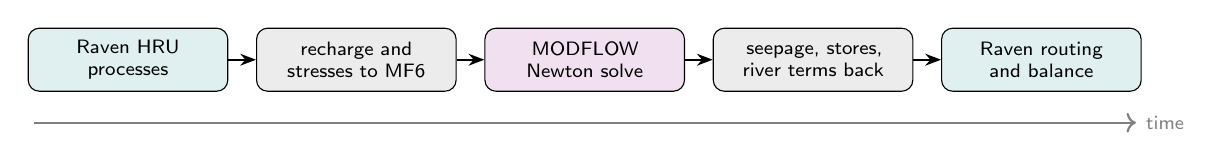
\begin{tikzpicture}[x=1cm,y=1cm,b/.style={draw,rounded corners,font=\scriptsize,align=center,minimum height=8mm,text width=23mm}]
\node[b,fill=teal!12] (a) at (0,0) {Raven HRU\\processes};
\node[b,fill=gray!15] (b) at (2.9,0) {recharge and\\stresses to MF6};
\node[b,fill=violet!12] (c) at (5.8,0) {MODFLOW\\Newton solve};
\node[b,fill=gray!15] (d) at (8.7,0) {seepage, stores,\\river terms back};
\node[b,fill=teal!12] (e) at (11.6,0) {Raven routing\\and balance};
\foreach \u/\v in {a/b,b/c,c/d,d/e} \draw[-{Stealth[length=2mm]},thick] (\u) -- (\v);
\draw[->,thick,gray] (-1.2,-0.8) -- (12.8,-0.8) node[right,font=\scriptsize]{time};
\end{tikzpicture}
\caption{Order of work within one time step.}\label{fig:timeline}
\end{figure}

Algorithm~\ref{alg:step} lists exactly what happens in one Raven time step of a coupled model.

\begin{algorithm}[!htbp]\caption{One coupled time step}\label{alg:step}
\begin{algorithmic}[1]
\State Raven: vertical and lateral processes of all HRUs; coupled HRUs' \cmd{GROUNDWATER} then holds the day's recharge
\State Complete yesterday's line of \cmd{GWBudget.csv} (river and reservoir terms are final only after routing)
\State Recharge: delay reservoirs (Ch.~\ref{ch:recharge}); spread over cells; skip fixed-head cells
\State MODFLOW \cmd{prepare\_time\_step}; set RCH rates
\State Set river stages and conductances, well rates, GHB/CHD heads (Ch.~\ref{ch:rivers},\ref{ch:wells})
\State Set water-table ET rates from PET left unmet by Raven (Ch.~\ref{ch:et})
\State Deliver yesterday's reservoir seepage (Ch.~\ref{ch:reservoirs}); set surface-store levels and limited conductances (Ch.~\ref{ch:stores})
\State \cmd{:SoilZone PHYSICAL}: share Raven's soil changes among the soil-zone columns; connected fractions, rejected recharge, local solves, \cmd{SZX\_RAVEN} boundaries (Ch.~\ref{ch:soilzone})
\State MODFLOW \cmd{prepare\_solve}; \textbf{repeat} \cmd{solve} (with \cmd{:SoilZone PHYSICAL}: then update the soil-zone interface) \textbf{until} converged or the iteration limit; \cmd{finalize\_solve}; \cmd{finalize\_time\_step}
\State Compute every package flow as $\mathrm{HCOF}\cdot h-\mathrm{RHS}$; reservoir local heads for today's routing
\State Surface-store exchange applied to Raven stores; seepage and river flows computed
\If{\cmd{:SoilZone PHYSICAL}} withhold from all discharge to Raven (seepage, gains, soil-zone inflow), in proportion, the soil-zone shortfall the booking would leave and, if the step did not converge, MODFLOW's negative residual; warn
\ElsIf{the step did not converge} withhold MODFLOW's negative residual from all discharge to Raven (seepage, river and store gains), in proportion; warn (first ten) \EndIf
\State \cmd{:SoilZone PHYSICAL}: MODFLOW's soil-zone flows and the rejected recharge applied to the columns; overflow to \cmd{SURFACE\_WATER}
\State Seepage added to Raven stores; balance, heads, connectivity and NetCDF output written
\State Raven: before routing, river gains added to / losses taken from each subbasin's in-catchment inflow
\State Raven routing; losses not covered are taken from the flow entering each reach; reservoirs compute seepage
\State Raven: water balance (recharge out, all returned water in); diagnostics including \cmd{GW\_HEAD}
\end{algorithmic}
\end{algorithm}

\subsection{Starting conditions}\label{sec:init}
Initial heads are chosen in this order: (1) a hotstart block \cmd{:GWHeads} in the \cmd{.rvc} file; (2)
\cmd{:InitialGWHeads} in the \cmd{.rvc} file (\cmd{DEPTH\_BELOW\_SURFACE d} or \cmd{ELEVATION z}); (3) each profile's
\cmd{INITIAL\_HEAD\_DEPTH}. Guessed initial heads can be far from reality; \cmd{:GWInitialization STEADY\_STATE r}
first solves a steady state before Raven's first day, with recharge $r$ [mm/d] over the area covered by coupled HRUs
(cell $i$ receives $r\,A^{\mathrm{cov}}_i/1000$ m$^3$/d, Section~\ref{sec:linkage}) and the initial river stages, well rates and boundary heads. This is skipped on a hotstart. A steady state may not
exist --- for example when wells pump more than the aquifer can supply --- and then the solve does not converge; Raven
warns and starts from the initial heads instead, as if \cmd{:GWInitialization} had not been given. The groundwater model is built after \emph{all} input files,
including the \cmd{.rvc}, have been read.

\subsection{Restarting a run (hotstart)}
At the end of a run Raven writes \cmd{solution.rvc}. Besides Raven's own states it contains \cmd{:GWHeads} (the head in
every cell), \cmd{:GWRechargeStore} (recharge delay stores, if used), \cmd{:GWRiverLossCarry} (river loss carried, if any) and \cmd{:GWReservoirSeepage} (reservoir seepage in
transit, if used), and with \cmd{:SoilZone PHYSICAL} \cmd{:GWSoilZoneColumns} (the water of every soil-zone column), and with unsaturated columns \cmd{:GWVadoseColumns} (\cmd{:GWVadoseClassColumns} with depth classes) and \cmd{:GWVadoseColumnTops} (each column's top and water). Using this file as the \cmd{.rvc} of a new run --- with \cmd{:StartDate} set to the end of the first
run --- continues exactly: in the tests the restarted run matched a continuous run to within $6\times10^{-6}$ in all flows.
Two details make this hold:
\begin{itemize}
\item Without \cmd{:SoilZone PHYSICAL}, seepage is added to its target store (\cmd{:SeepageReturnTo}, by default the
lowest soil layer) with no capacity limit, so that layer can hold more than its capacity for a while. On reading the
\cmd{.rvc}, Raven cuts every state above its maximum back to the maximum; for the seepage target of a coupled HRU it keeps
the value as written, so the restart carries the same water as the continuous run. The same holds for the store of a
\cmd{:SurfaceWaterExchange} (for example \cmd{DEPRESSION} above \cmd{DEP\_MAX}), which groundwater discharge fills with no
capacity limit.
\item The unsaturated columns are restored with the contents as written (\cmd{:GWVadoseColumns},
\cmd{:GWVadoseClassColumns}), floored only at what the method can hold: the air-dry content
$\theta(\psi=-10^5$\,m$)$ for \cmd{RICHARDS} and \cmd{LAG}, zero for \cmd{KINEMATIC} (whose reference content
$\theta_s-S_y$ can lie below air-dry when $S_y$ is close to the porosity). A line is used only for a column with the same
top (within 1~mm, \cmd{:GWVadoseColumnTops}), the same number of nodes and the same depth classes; another column starts at
rest (its reference profile), with a warning. A run without unsaturated columns (\cmd{:SoilZoneVadose NONE}, or no
\cmd{:SoilZone PHYSICAL}) cannot hold the columns' water: it warns, and \cmd{GWModelSummary.txt} reports the lines and their
water (above the columns' reference profiles) as dropped.
\end{itemize}
In Raven runs without groundwater, an age tracer (\cmd{:Transport AGE}; transport is not available in a coupled run,
Section~\ref{ch:inputs}) is restarted as follows. The file's tracer masses are volumes times entry times counted from a
datum: the start of the first run of a chain of restarts. \cmd{:StartTime} in \cmd{solution.rvc} is the start of the run that
wrote it; when the datum is earlier, the file also carries \cmd{:AgeTracerDatum} with that date. A run read from the file
counts its ages from \cmd{:AgeTracerDatum}, else from \cmd{:StartTime} when the file holds age-tracer masses; from a file
without them (a spin-up run without the tracer) the initial water has age 0.

Damaged groundwater values in the \cmd{.rvc} stop the run with a message naming the block: a value that is not a finite
number in any groundwater block, and negative water in \cmd{:GWSoilZoneColumns}, \cmd{:GWVadoseColumns} or
\cmd{:GWVadoseClassColumns}.

\subsection{Ensembles}
Raven's ensemble modes (Monte Carlo, DDS, EnKF) run the model several times in one program run. For every member the
groundwater model is rebuilt from scratch, MODFLOW is restarted, and its files go to that member's output folder.
Each member starts with a fresh water balance and, unless its own \cmd{.rvc} says
otherwise, from the routing memory and reservoir states of the first run (stage, outflow, loss terms). These defaults are
restored before the member's \cmd{.rvc} is read, so member-specific initial conditions (as used by EnKF forecasting) still
apply; groundwater hotstart values are likewise cleared, so each member uses only its own \cmd{.rvc}, and the steady-state
start is decided for each member separately
(Section~\ref{sec:coreflix}). An EnKF member's own time series file (\cmd{:ExtraRVTFilename}) may give
\cmd{:WellFlowRate} and \cmd{:BoundaryHead} series: they replace, for that member and the later ones, the series of the
same well or boundary read before, and a series naming no well or boundary stops the run.

\subsection{Safeguards}\label{sec:guard}
\begin{itemize}
\item \textbf{Non-converged steps.} Raven carries such a step on with MODFLOW's flows, as MODFLOW's own
\cmd{CONTINUE} option would: every flow MODFLOW booked is applied, and only its residual is not. A negative residual
(more outflow booked than the inflows and the storage release supply) is withheld from all discharge returned to Raven
--- seepage, river gains, discharge into wetland and lake stores, and with \cmd{:SoilZone PHYSICAL} the inflow to the
soil zone --- in proportion; what that discharge cannot cover stays in the aquifer. The withheld water is MODFLOW's
balance error of the step. Without \cmd{:SoilZone PHYSICAL}, the discharge columns of \cmd{GWBudget.csv} on such a step
(``seepage to Raven'', ``aquifer discharge to rivers'', ``aquifer discharge to surface stores'') give the discharge
handed to Raven, after the withholding, so each row's residual --- recharge plus storage release plus the other inflows,
less the discharge, less ``MF6 balance error'' --- is the volume withheld in that step; its run total is in
\cmd{GWModelSummary.txt} (``discharge withheld''). With \cmd{:SoilZone PHYSICAL} the withheld volume is booked per step
in its own columns of \cmd{GWBudget.csv} (seepage and soil inflow, river gains and surface-store gains withheld). The step is
flagged, and a warning written for the first ten such steps (test B8, Table~\ref{tab:vszinterface}).
\item \textbf{Rivers and stores} can never lose more water than they hold (Sections~\ref{ch:rivers},\ref{ch:stores}).
\item \textbf{Wells} cannot pump from a dry cell (\cmd{AUTO\_FLOW\_REDUCE}).
\item \textbf{Step count}: Raven stops if it would run past MODFLOW's last step.
\item \textbf{MODFLOW folder}: if Raven cannot enter the MODFLOW folder, the call fails with a clear message instead of
running MODFLOW in the wrong place.
\end{itemize}


\chapter{Inputs and outputs}\label{ch:c6}
This chapter is the reference for every command and every output, followed by a complete example set-up.

\begin{plain}
This is the look-up chapter: every command you can write in the input files, what it does and its default, and every output
file with its columns. There is no need to read it from start to finish; come here when you need the exact spelling of a
command or the meaning of an output column.
\end{plain}

\section{Input reference}\label{ch:inputs}
This chapter lists every command. Commands are case sensitive; separators may be commas or spaces, as in all Raven files.

\subsection{\texttt{.rvi} (main input file)}
\begin{table}[!htbp]\centering
\caption{Commands in the \cmd{.rvi} file.}
\begin{tabular}{P{0.34\linewidth}P{0.608\linewidth}}\toprule\hdr
Command & Meaning\\\midrule
\cmd{:GroundwaterModel MODFLOW6} & switches the coupling on (\cmd{NONE}: off, the default)\\
\cmd{:rvg\_Filename file} & name of the groundwater file, relative to the \cmd{.rvi} (default \cmd{<model>.rvg})\\
processes into \cmd{GROUNDWATER} & any process moving water into \cmd{GROUNDWATER} in a coupled HRU produces recharge; use
\cmd{:-->Conditional HRU\_GROUP} so uncoupled HRUs keep their own baseflow\\
\cmd{:Transport} & not available with \cmd{:GroundwaterModel MODFLOW6}: the coupling exchanges water only, no
constituent mass (recharge would leave its mass in Raven's \cmd{GROUNDWATER} store, and seepage and groundwater discharge
would return water without mass), so a coupled run with any \cmd{:Transport} command (including \cmd{AGE} and
\cmd{TEMPERATURE}) stops with a message naming the constituent\\\bottomrule
\end{tabular}
\end{table}

\subsection{\texttt{.rvh} (HRUs and subbasins)}
The existing \cmd{AQUIFER\_PROFILE} column of \cmd{:HRUs} holds a profile name, or \cmd{[NONE]}. Reservoirs to be coupled
need \cmd{:SeepageParameters} and a lake HRU (\cmd{:HRUID}) with an \cmd{AQUIFER\_PROFILE}.

\subsection{\texttt{.rvp} (parameters)}
\begin{lstlisting}
:AquiferClasses
  :Attributes, K_HORIZ, K_VERT, SPEC_STORAGE, SPEC_YIELD, POROSITY
  :Units,      m/d,     m/d,    1/m,          none,       none
  GRAVEL,      50.0,    5.0,    1.0E-5,       0.25,       0.30
  CLAY_TILL,   0.001,   0.0001, 1.0E-4,       0.03,       0.40
:EndAquiferClasses
:AquiferProfiles
  # name, number of layers, then {class, thickness [m] or TO_BEDROCK, layer type} for each layer
  VALLEY_ALLUVIUM, 3, GRAVEL, 15.0, AQUIFER, CLAY_TILL, 5.0, AQUITARD, SAND, TO_BEDROCK, CONFINED_AQUIFER
  UPLAND_TILL,     1, UPLAND_TILL, TO_BEDROCK, AQUIFER
:EndAquiferProfiles
:AquiferProfileParameters
  :Attributes,     INITIAL_HEAD_DEPTH, SEEPAGE_LEAKANCE, RECHARGE_DELAY
  :Units,          m,                  1/d,              d
  VALLEY_ALLUVIUM, 3.0,                1.0,              0.0
:EndAquiferProfileParameters
\end{lstlisting}
\begin{table}[!htbp]\centering
\caption{Aquifer class attributes (\cmd{.rvp}).}
\begin{tabular}{P{0.27\linewidth}P{0.13\linewidth}P{0.528\linewidth}}\toprule\hdr
Aquifer class attribute & Default & Meaning\\\midrule
\cmd{K\_HORIZ} & required & horizontal hydraulic conductivity [m/d]\\
\cmd{K\_VERT} & $K_h/10$ & vertical hydraulic conductivity [m/d]\\
\cmd{SPEC\_STORAGE} & $10^{-5}$ & specific storage [1/m]\\
\cmd{SPEC\_YIELD} & 0.1 & specific yield [--]\\
\cmd{POROSITY} & 0.3 & saturated water content $\theta_s$ of the unsaturated columns [--] (\cmd{:SoilZoneVadose}; at least \cmd{SPEC\_YIELD})\\
\cmd{CLAPP\_B} & 4 & Clapp--Hornberger exponent $b$ of the unsaturated columns [--]\\
\cmd{AIR\_ENTRY\_PRESSURE} & 0.3 m & air-entry suction $\psi_a$ of the unsaturated columns [m]\\\bottomrule
\end{tabular}
\end{table}
Layer types: \cmd{AQUIFER} (or \cmd{UNCONFINED\_AQUIFER}), \cmd{CONFINED\_AQUIFER}, \cmd{AQUITARD},
\cmd{AQUICLUDE} (not as top layer). Classes must be defined before the profiles that use them.
With \cmd{:MF6Simulation} a profile may have no layers (\cmd{name, 0}); the model's own layers are used.
\begin{table}[!htbp]\centering
\caption{Aquifer profile parameters (\cmd{.rvp}).}
\begin{tabular}{P{0.3\linewidth}P{0.13\linewidth}P{0.498\linewidth}}\toprule\hdr
Profile parameter & Default & Meaning\\\midrule
\cmd{INITIAL\_HEAD\_DEPTH} & 5 m & initial depth to water below land surface\\
\cmd{DEFAULT\_BEDROCK\_DEPTH} & 50 m & bedrock depth where no bedrock map is given\\
\cmd{SOIL\_ZONE\_DEPTH} & 0 m & model top below land surface\\
\cmd{SEEPAGE\_LEAKANCE} & 1 d$^{-1}$ & seepage conductance per m$^2$ of cell\\
\cmd{SEEPAGE\_SMOOTHING\_DEPTH} & 0.5 m & depth below the top where seepage starts\\
\cmd{RIVERBED\_K} & 0.5 m/d & riverbed hydraulic conductivity\\
\cmd{RIVERBED\_THICKNESS} & 1 m & riverbed thickness\\
\cmd{EXTINCTION\_DEPTH} & 0 m & water-table ET extinction depth (0 = off)\\
\cmd{RECHARGE\_DELAY} & 0 d & recharge delay time constant (0 = off)\\\bottomrule
\end{tabular}
\end{table}

\subsection{\texttt{.rvg} (groundwater file)}
\begin{longtable}{P{0.45\linewidth}P{0.498\linewidth}}
\caption{Commands in the \cmd{.rvg} file.}\\
\toprule\hdr
Command & Meaning (default)\\\midrule\endfirsthead
\caption[]{Commands in the \cmd{.rvg} file (continued).}\\
\toprule\hdr
Command & Meaning (default)\\\midrule\endhead
\cmd{:HRUGeometry file \{ID field\}} & HRU polygons, GeoJSON in lon/lat (or \cmd{:InputCRS}); ID field (\cmd{HRU\_ID}). \textbf{Required.}\\
\cmd{:RiverGeometry file \{subbasin field\}} & river lines; without a field, subbasins are assigned automatically\\
\cmd{:LandSurface file} & DEM, ESRI ASCII grid or GeoTIFF (\cmd{.tif}, \cmd{.tiff}) in lon/lat or \cmd{:InputCRS}; Section~\ref{sec:rasters} (HRU \cmd{ELEVATION})\\
\cmd{:InputCRS EPSG:code | TMERC | ALBERS | LCC \dots} & projection of every geometry and raster input file; wells may then be given by \cmd{X}, \cmd{Y} (lon/lat); Section~\ref{sec:inputcrs}\\
\cmd{:BedrockSurface file} & bedrock elevation, same formats (\cmd{DEFAULT\_BEDROCK\_DEPTH})\\
\cmd{:GridCellSize m} & cell size (1000 m)\\
\cmd{:MinCellCoverage f} & fraction of a cell that coupled HRUs must cover (0.25)\\
\cmd{:GridType REGULAR|QUADTREE|HRU\_MESH|FILE} & kind of grid (\cmd{REGULAR}); Section~\ref{sec:gridtypes}\\
\cmd{:MF6Simulation file} & couple an existing MODFLOW 6 simulation (Chapter~\ref{ch:existing})\\
\cmd{:MF6Model}, \cmd{:MF6StartDate} & model to couple (if several); date of the model's time zero\\
\cmd{:MF6CRS}, \cmd{:MF6GridFile}, \cmd{:OverlapWeights} & how HRUs are linked to the model's cells (one of them)\\
\cmd{:RavenTakesOver}, \cmd{:KeepPackages} & recharge/ET/UZF packages replaced by Raven or kept\\
\cmd{:StreamPackage p \{AUX a|DOMINANT\_HRU\}}, \cmd{:SeepageToRaven ON|OFF} & stream package to Raven's reaches; seepage package\\
\cmd{:GridRotation} $\theta$ & rotation of regular and quadtree grids, degrees counterclockwise (0)\\
\cmd{:GridRefinement RIVERS|WELLS|LAKES s}, \cmd{LINES|POLYGONS file s} & finer cells (size $s$ [m]) along rivers, around wells, in and around reservoir lakes, or along/around features in a file\\
\cmd{:GridFile file \{ID\}} & imported cell polygons, with \cmd{:GridType FILE} (ID field \cmd{CELL\_ID})\\
\cmd{:QuadtreeMaxLevel n} & maximum halvings of the base cell (from the refinement sizes)\\
\cmd{:FlowCorrection AUTO|XT3D|XT3D\_RHS|NONE} & XT3D conductance tensor (\cmd{AUTO}: off; \cmd{XT3D\_RHS} or \cmd{XT3D} to switch it on)\\
\cmd{:LayerConnection INDEX|ELEVATION} & connect layers by number or by overlapping elevation (\cmd{INDEX})\\
\cmd{:MF6Library path} & MODFLOW 6 library (else the environment variable \cmd{RAVEN\_MF6\_LIB}, next to the Raven executable, then \cmd{lib/mf6/} of the Raven checkout, then the system path; Section~\ref{sec:getmf6})\\
\cmd{:SeepageReturnTo SV} & Raven store receiving seepage (lowest soil layer; soil-less HRUs: \cmd{SURFACE\_WATER})\\
\cmd{:RiverBedDepth m | REFERENCE\_FLOW} & riverbed depth below the DEM (\cmd{REFERENCE\_FLOW})\\
\cmd{:GWInitialization STEADY\_STATE r} & steady-state start with recharge $r$ mm/d (off)\\
\cmd{:SurfaceWater\allowbreak Exchange SV group LEAKANCE L} & Raven store of an HRU group $\leftrightarrow$ aquifer (also with \cmd{:MF6Simulation})\\
\cmd{:ReservoirExchange} & Raven reservoirs $\leftrightarrow$ aquifer (also with \cmd{:MF6Simulation})\\
\cmd{:Wells} \dots\ \cmd{:EndWells} & table: ID, \cmd{NAME, LATITUDE, LONGITUDE, SCREEN\_TOP, SCREEN\_BOT} (with \cmd{:InputCRS}: \cmd{X, Y} instead of \cmd{LATITUDE, LONGITUDE})\\
\cmd{:ObservationWells} \dots & table: ID, \cmd{NAME, LATITUDE, LONGITUDE, SCREEN\_ELEV} (or \cmd{X, Y})\\
\cmd{:GeneralHeadBoundary name file HEAD h CONDUCTANCE c \{LAYERS ALL|TOP\}} & head-dependent boundary; $c$ per cell [m$^2$/d]\\
\cmd{:SpecifiedHeadBoundary name file HEAD h \{LAYERS ALL|TOP\}} & fixed-head boundary\\
\cmd{:SolverMax\allowbreak OuterIterations n} & Newton iterations per step (500)\\
\cmd{:SolverHead\allowbreak Tolerance m} & Newton head-change tolerance (0.00001 m)\\
\cmd{:HeadSaveFrequency n} & steps between saves of the full head field (30)\\
\cmd{:WriteNetCDFHeads} & write \cmd{GWHeads.nc} (Raven compiled with NetCDF)\\
\cmd{:WriteGWBudgetFile} & MODFLOW budget file \cmd{mf6/gwf.cbc} and \cmd{mf6/gwf.porosity} for particle tracking (off; generated models; Section~\ref{sec:budgetfile})\\
\cmd{:LinkageCache file} & linkage cache location (\cmd{<output>/mf6/linkage.cache})\\
\cmd{:SoilZone CONCEPTUAL | PHYSICAL SOIL[0] \dots} & the soil zone and the water table (\cmd{CONCEPTUAL}); with \cmd{PHYSICAL} the further \cmd{:SoilZone*} commands of Table~\ref{tab:szcmds} apply\\\bottomrule
\end{longtable}

\subsection{Soil-zone commands (\texttt{.rvg})}\label{sec:szcmdref}
These commands apply only with \cmd{:SoilZone PHYSICAL} (Section~\ref{ch:soilzone}); without it they are reported as
ignored. A command given where it has no effect (\cmd{:SoilZoneVadoseClasses} or \cmd{:SoilZoneVadoseInitialFlux} with
\cmd{:SoilZoneVadose NONE}, \cmd{:SoilZoneAquiferClass} on a model Raven builds) is reported as ignored too. Values
outside the ranges given stop the run with a message.
\begin{longtable}{P{0.36\linewidth}P{0.15\linewidth}P{0.42\linewidth}}
\caption{Soil-zone commands in the \cmd{.rvg} file.}\label{tab:szcmds}\\
\toprule\hdr Command and syntax & Default & Meaning\\\midrule\endfirsthead
\caption[]{Soil-zone commands in the \cmd{.rvg} file (continued).}\\
\toprule\hdr Command and syntax & Default & Meaning\\\midrule\endhead
\cmd{:SoilZone CONCEPTUAL} \newline \cmd{:SoilZone PHYSICAL SOIL[0] \dots\ SOIL[$M-1$]} & \cmd{CONCEPTUAL} & \cmd{PHYSICAL}: the listed soil layers (from the top, consecutive) are the soil zone, owned by Raven; MODFLOW starts below them and the water table may rise into them (Section~\ref{ch:soilzone}). The last \cmd{:SoilZone} counts\\
\cmd{:SoilZoneIteration n \{$\epsilon_h$\} \{tol$_Q$\}} & 100, 0.0001~m, 0.000001 & interface updates after MODFLOW's outer iterations, $n\ge0$ (0: explicit coupling); soil-level tolerance [m] and relative flow tolerance, $>0$ (Section~\ref{sec:szinterface})\\
\cmd{:SoilZoneSubgrid n} & 5 & DEM points per cell side ($n^2$ points per cell) for the saturated fraction on sloping and irregular land, $1\le n\le20$ (Section~\ref{sec:szslope})\\
\cmd{:SoilZoneOutput group} & all soil-zone HRUs & HRU group written to \cmd{GWSoilExchange.csv}\\
\cmd{:SoilZoneVadose NONE} \newline \cmd{:SoilZoneVadose RICHARDS \{$\epsilon$\} \{N\}} \newline \cmd{:SoilZoneVadose KINEMATIC \{$\epsilon$\} \{N\}} \newline \cmd{:SoilZoneVadose LAG \{$t_m$\} \{N\}} & \cmd{NONE}; $\epsilon$ 0.02, $t_m$ 0, $N$ 16 & unsaturated columns between the soil-zone base and a deeper water table: Richards' equation, kinematic wave or linear storage cascade (Sections~\ref{sec:szvadose}, \ref{sec:szvadosekw}, \ref{sec:szvadoselag}); $\epsilon$ largest content change in a substep, $(0,0.2]$; $t_m$ travel time per metre [d/m], $\ge0$ (0: derived from each material); $N$ nodes per column at most, 3 to 200. \cmd{NONE}: recharge reaches the water table in the step\\
\cmd{:SoilZoneVadoseClasses K} & 1 & unsaturated columns per exchange column, one per depth class of its DEM points, $1\le K\le10$ (Section~\ref{sec:vzclasses})\\
\cmd{:SoilZoneVadoseInitialFlux q} & 0 & on a cold start, every unsaturated column starts at its steady profile for the flux it receives, $(1-F)\,q$, $q\ge0$ [mm/d]; 0: at rest (reference profile); ignored on a groundwater hotstart\\
\cmd{:SoilZoneCapillaryRise ON | OFF} & \cmd{ON} with \cmd{RICHARDS}, \cmd{KINEMATIC} or \cmd{LAG}; \cmd{OFF} with \cmd{NONE} & capillary rise from the water table (and, with \cmd{RICHARDS}, from the columns' top nodes) into soil-zone layers below field capacity (Section~\ref{sec:szcaprise})\\
\cmd{:SoilZoneExchangeTiming LAGGED | AFTER} & \cmd{LAGGED} & \cmd{LAGGED}: last step's exchange is lent to the soil zone before Raven's processes and settled after the step's exchange; \cmd{AFTER}: the exchange follows Raven's processes (Section~\ref{sec:sztiming})\\
\cmd{:SoilZoneClasses K} & 1 & Raven's processes run on up to $K$ wetness classes of each HRU's soil-zone columns, $1\le K\le50$; needs \cmd{:Method ORDERED\_SERIES} (Section~\ref{sec:szclasses})\\
\cmd{:SoilZoneAquiferClass class} & $b$ 4, $\psi_a$ 0.3~m, $\theta_s$ $S_y+0.1$ & existing models only: the aquifer class whose \cmd{CLAPP\_B}, \cmd{AIR\_ENTRY\_PRESSURE} and \cmd{POROSITY} the unsaturated columns use (conductivity and specific yield come from the model; a steady model without specific yield takes the class's \cmd{SPEC\_YIELD} when given, else 0.2; Section~\ref{sec:szexisting})\\\bottomrule
\end{longtable}
The soil classes of the soil-zone layers need \cmd{POROSITY}, \cmd{FIELD\_CAPACITY} $<1$, and, for the bottom layer,
\cmd{HYDRAUL\_COND} [mm/d]; capillary rise uses their \cmd{CLAPP\_B} and \cmd{AIR\_ENTRY\_PRESSURE} [mm]. Recharge must leave the
soil zone from \cmd{SOIL[$M-1$]} into \cmd{GROUNDWATER}, and \cmd{RECHARGE\_DELAY} must be 0 for soil-zone HRUs (a delay through a
deep unsaturated zone: \cmd{:SoilZoneVadose LAG}, Section~\ref{sec:szvadoselag}). The
aquifer profile parameter \cmd{SEEPAGE\_SMOOTHING\_DEPTH} is the contact depth $d_s$ of the soil zone (below 0.1~m a
warning); \cmd{SOIL\_ZONE\_DEPTH} and \cmd{SEEPAGE\_LEAKANCE} are not used for soil-zone HRUs.
The block commands take one row per item, for example:
\begin{lstlisting}
:Wells
  :Attributes, NAME, LATITUDE, LONGITUDE, SCREEN_TOP, SCREEN_BOT
  1, PW_1, 59.27310, -124.73460, 1199.7, 1188.7
:EndWells
:ObservationWells
  :Attributes, NAME, LATITUDE, LONGITUDE, SCREEN_ELEV
  101, OW_NEAR, 59.27310, -124.73060, 1192.7
:EndObservationWells
:GeneralHeadBoundary   GHB1  boundary_line.geojson HEAD 1310.0 CONDUCTANCE 5000.0 LAYERS TOP
:SpecifiedHeadBoundary LAKE1 lake.geojson          HEAD 1312.0 LAYERS TOP
:SurfaceWaterExchange  DEPRESSION WetlandHRUs LEAKANCE 0.01
:ReservoirExchange
\end{lstlisting}

\subsection{\texttt{.rvt} (time series)}
\begin{lstlisting}
:WellFlowRate 1 m3/d                  # well ID; negative = pumping
  1985-10-01 00:00:00 1.0 1826
  0.0
  ...
:EndWellFlowRate
:BoundaryHead GHB1 m              # replaces HEAD of boundary GHB1
  1985-10-01 00:00:00 1.0 1826
  ...
:EndBoundaryHead
:ObservationData GW_HEAD 101 m    # observation-well ID; head AT each date
  1985-10-01 00:00:00 1.0 1826
  ...
:EndObservationData
\end{lstlisting}

\subsection{\texttt{.rvc} (initial conditions)}
\par\noindent\begin{minipage}{\linewidth}
\begin{lstlisting}
:InitialGWHeads DEPTH_BELOW_SURFACE 5.0     # or FROM_PROFILE (default) or ELEVATION z
\end{lstlisting}
\end{minipage}\par\smallskip
\cmd{:GWHeads nlay nrow ncol}, \cmd{:GWRechargeStore}, \cmd{:GWRiverLossCarry} and \cmd{:GWReservoirSeepage}, and with
\cmd{:SoilZone PHYSICAL} \cmd{:GWSoilZoneColumns}, \cmd{:GWVadoseColumns}, \cmd{:GWVadoseClassColumns} and \cmd{:GWSoilZoneLag},
are written by Raven into \cmd{solution.rvc} for hotstart; they are read back automatically (Section~\ref{app:hotstart}).

\section{Output reference}\label{ch:outputs}
All rows are stamped with the date at the \emph{end} of the step (the moment the values refer to).
\subsection{\texttt{GWBudget.csv} --- one row per step}
\begin{table}[!htbp]\centering
\caption{Columns of \cmd{GWBudget.csv}.}
\begin{tabular}{P{0.43\linewidth}P{0.518\linewidth}}\toprule\hdr
Column & Meaning\\\midrule
time, date & model time [d] and date at the end of the step\\
Raven recharge [m$^3$/d] & recharge leaving Raven (before any delay)\\
MF6 recharge [m$^3$/d] & recharge entering MODFLOW\\
seepage to Raven [m$^3$/d] & drain discharge at the model top\\
storage release [m$^3$/d] & water released from aquifer storage (negative: stored)\\
MF6 balance error [m$^3$/d], [\%] & $\varepsilon$ of Section~\ref{ch:balance}, and relative to gross flow\\
returned to Raven [m$^3$] & seepage volume added to Raven stores\\
outer iterations, converged & Newton iterations used; 1 target tolerance reached, 2 accepted at the relaxed tolerance, 0 not converged\\
recharge delay storage [m$^3$] & water in delay reservoirs\\
recharge onto CHD cells [m$^3$/d] & recharge of HRUs lying entirely on fixed-head cells\\
river leakage to aquifer, aquifer discharge to rivers [m$^3$/d] & river exchange, each direction (on a step MODFLOW did not converge, without \cmd{:SoilZone PHYSICAL}: the discharge handed to Raven, after the withholding of Section~\ref{sec:guard}; so are \emph{seepage to Raven} and \emph{aquifer discharge to surface stores})\\
river exchange applied to Raven [m$^3$] & net volume actually added to (or taken from) Raven reaches\\
river loss carried to next step [m$^3$] & river loss not supplied in the step, taken from the river the next step (normally 0)\\
water-table ET [m$^3$/d] & evaporation from the water table\\
wells specified, wells actual [m$^3$/d] & requested and delivered well rates\\
GHB, CHD [m$^3$/d] & boundary flows (positive into the aquifer)\\
surface-store leakage / discharge [m$^3$/d], applied [m$^3$] & wetland and lake exchange\\
reservoir seepage sent, delivered [m$^3$/d], awaiting delivery [m$^3$] & reservoir exchange\\
reservoir gain not supplied by MODFLOW [m$^3$] & a gain the lake received that MODFLOW did not supply (a drying cell, or cells under the lake that were specified heads or inactive on the day it was delivered); taken back from the water reaching the subbasin in the same step (normally 0; a warning and a run total)\\
other model packages [m$^3$/d] & with an existing model: net flow of the model's own packages (wells, boundaries, \dots), positive into the aquifer\\
soil zone to aquifer, aquifer to soil zone [m$^3$/d] & \cmd{:SoilZone PHYSICAL}: soil-zone exchange, each direction\\
rejected recharge, soil-zone overflow, exchange applied to Raven, shortfall [m$^3$] & Section~\ref{ch:soilzone}; shortfall is 0 (except on steps MODFLOW ended unconverged at a low outer-iteration limit)\\
interface updates, converged, change [m] & soil-zone interface iteration of the step\\
further soil-zone columns & layer redistribution, withheld discharge, negative recharge not held, unsaturated zone (inflow, to aquifer, capillary rise, storage), capillary rise from the water table, lagged-exchange debt and repayment, specified-head exchange, recharge not applied, reservoir seepage not delivered: Section~\ref{app:outputs}\\\bottomrule
\end{tabular}
\end{table}

\noindent One row of \cmd{GWBudget.csv} from the 20-year Liard run (selected columns):
\begin{center}\small
\begin{tabular}{ll}\toprule\hdr
Column & Value\\\midrule
\cmd{time [d]}, \cmd{date} & 3910, 1996-06-15\\
\cmd{Raven recharge [m3/d]} & 21\,365\,037.27\\
\cmd{MF6 recharge [m3/d]} & 21\,365\,037.27\\
\cmd{seepage to Raven [m3/d]} & 19\,087\,056.98\\
\cmd{storage release [m3/d]} & $-3\,925\,200.44$\\\bottomrule
\end{tabular}
\end{center}
Recharge leaving Raven equals recharge entering MODFLOW; on this wet June day the aquifer stores about 3.9 million m$^3$.

\subsection{Other files}
\begin{table}[!htbp]\centering
\caption{Other output files.}\label{tab:outputs}
\begin{tabular}{P{0.25\linewidth}P{0.698\linewidth}}\toprule\hdr
File & Content\\\midrule
\cmd{GWHRUState.csv} & per coupled HRU: overlap-weighted mean water table of its columns and mean depth to water\\
\cmd{GWSoilExchange.csv} & \cmd{:SoilZone PHYSICAL}: per soil-zone HRU and step, soil-zone base, soil water level and water table (area means over all the HRU's soil-zone columns, those over specified-head cells included, whose water table is the specified head; empty for an HRU without a column), saturated fraction, exchange with the aquifer both ways (\emph{soil zone to aquifer}, \emph{aquifer to soil zone}: with active cells, as \cmd{GWBudget.csv} books it), rejected recharge, overflow, soil water and capacity; in a model with specified heads also \emph{soil zone to specified heads} and \emph{specified heads to soil zone} (columns over specified-head cells and links whose cell is a specified head in the step, with the capillary rise a specified head supplies). Summed over the HRUs, each exchange column equals the column of the same name in \cmd{GWBudget.csv} (Section~\ref{ch:soilzone}). Two further columns are model-wide values of the step, repeated on every HRU's row: \emph{interface updates} and \emph{interface change [m]} (as in \cmd{GWBudget.csv})\\
\cmd{GWHeads.csv} & head at each monitoring well, from $t=0$ (missing value $-1.2345$ when the screened cell is dry)\\
\cmd{GWConnectivity.csv} & number of separate wet areas; wet fraction of each profile\\
\cmd{mf6/grid\_cells.geojson} & every cell as a lon/lat polygon: number, active, profile, dominant HRU, area\\
\cmd{GWModelSummary.txt} & MODFLOW 6 library and its version, grid type and size, MODFLOW format, HRU fidelity of the cells, active and pass-through cells, profiles, river/well/boundary/store/reservoir cells, linkage per HRU (areas, fraction linked, cells), whether the linkage came from the cache\\
\cmd{GWHeads.nc} & (optional) head(time, layer, y, x) with 2-D latitude and longitude, CF conventions\\
\cmd{mf6/} & the generated MODFLOW model, its list file (\cmd{gwf.lst}, \cmd{mfsim.lst}) and binary heads (\cmd{gwf.hds}); with \cmd{:WriteGWBudgetFile} also the budget file \cmd{gwf.cbc} and \cmd{gwf.porosity}\\
\cmd{Diagnostics.csv} & Raven's usual file, with \cmd{GW\_HEAD} statistics\\
\cmd{Watershed\allowbreak Storage.csv} & Raven's balance; includes all exchanged water\\
\cmd{solution.rvc} & includes \cmd{:GWHeads}, \cmd{:GWRechargeStore}, \cmd{:GWReservoirSeepage}, \cmd{:GWRiverLossCarry}, \cmd{:GWSoilZoneColumns}, \cmd{:GWVadoseColumns}, \cmd{:GWVadoseClassColumns}, \cmd{:GWSoilZoneLag}\\\bottomrule
\end{tabular}
\end{table}

\subsection{Budget file and particle tracking}\label{sec:budgetfile}
With \cmd{:WriteGWBudgetFile} a generated model saves MODFLOW's cell-by-cell flows: the model's name file gets
\cmd{SAVE\_FLOWS} (every package), the NPF package \cmd{SAVE\_SPECIFIC\_DISCHARGE} and \cmd{SAVE\_SATURATION}, and the output
control writes \cmd{mf6/gwf.cbc} at the steps it saves the heads (\cmd{:HeadSaveFrequency}). \cmd{mf6/gwf.porosity} holds the
\cmd{POROSITY} of each cell's aquifer class in MODFLOW's array layout, written as the \cmd{GRIDDATA} block of a PRT \cmd{MIP6} file.
Nothing else changes: without the option the \cmd{mf6} folder is the same, and with it the solution is identical.

These files let MODFLOW~6's particle-tracking model (PRT) or MODPATH run on the coupled flows after the Raven run.
\cmd{tools/make\_prt.py OUTPUT\_FOLDER [-{}-backward] [-{}-points file] [-{}-run libmf6]} builds a PRT simulation in
\cmd{OUTPUT\_FOLDER/prt/}: release points around each well of \cmd{:Wells} (or from a file), the flow model's periods, and
the head and budget files, reversed with FloPy for backward tracking (capture zones and times of travel). With \cmd{-{}-run}
it runs PRT through the MODFLOW~6 library and writes \cmd{endpoints.csv} (travel time and end point of every particle). PRT
tracks particles on DIS and DISV grids (regular and quadtree grids); for tracking through time, save the flows every step
(\cmd{:HeadSaveFrequency 1}). An existing model keeps its own output control: add \cmd{BUDGET FILEOUT} and
\cmd{SAVE BUDGET} to its OC file instead (Chapter~\ref{ch:existing}).

\section{A complete example set-up}
The following \cmd{.rvg} uses most options (the soil-zone commands of Table~\ref{tab:szcmds} keep their defaults except those shown); lines not needed can be deleted. With \cmd{:SoilZone PHYSICAL} the \cmd{:SurfaceWaterExchange} group must not name a soil-zone layer (its \cmd{DEPRESSION} store lies on the ground above the soil zone, and its exchange has its bed there, Section~\ref{ch:stores}), and the \cmd{.rvi} takes recharge from \cmd{SOIL[1]}.
\begin{lstlisting}
# ---- geometry ----
:HRUGeometry        my_hrus.geojson   HRU_ID
:RiverGeometry      my_rivers.geojson SubId
:LandSurface        dem_lonlat.asc
:BedrockSurface     bedrock_lonlat.asc
# ---- grid and solver ----
:GridCellSize       1000.0
:MinCellCoverage    0.25
:SolverHeadTolerance 0.00001
:SolverMaxOuterIterations 500
:HeadSaveFrequency  30
:WriteNetCDFHeads
:LinkageCache       cache/linkage.cache
# ---- coupling options ----
:MF6Library         /opt/mf6/libmf6.so
:SeepageReturnTo    SOIL[2]
:RiverBedDepth      REFERENCE_FLOW
:GWInitialization   STEADY_STATE 0.5
:SurfaceWaterExchange DEPRESSION WetlandHRUs LEAKANCE 0.01
:ReservoirExchange
# ---- soil zone and water table (optional) ----
:SoilZone PHYSICAL SOIL[0] SOIL[1]
:SoilZoneVadose RICHARDS
:SoilZoneVadoseClasses 3
:SoilZoneClasses 3
# ---- stresses and observations ----
:Wells
  :Attributes, NAME, LATITUDE, LONGITUDE, SCREEN_TOP, SCREEN_BOT
  1, TownWell, 49.123, -80.456, 245.0, 230.0
:EndWells
:ObservationWells
  :Attributes, NAME, LATITUDE, LONGITUDE, SCREEN_ELEV
  101, OW_1, 49.120, -80.450, 240.0
:EndObservationWells
:GeneralHeadBoundary   East  east_edge.geojson HEAD 210.0 CONDUCTANCE 2000.0 LAYERS ALL
:SpecifiedHeadBoundary Lake  lake.geojson      HEAD 255.0 LAYERS TOP
\end{lstlisting}
with, in the \cmd{.rvt},
\begin{lstlisting}
:WellFlowRate 1 m3/d
  2000-01-01 00:00:00 1.0 3
  -1500.0
  -1500.0
  -1800.0
:EndWellFlowRate
:ObservationData GW_HEAD 101 m
  2000-01-01 00:00:00 1.0 3
  241.20
  241.18
  -1.2345
:EndObservationData
\end{lstlisting}
(\cmd{-1.2345} marks a missing observation, as elsewhere in Raven). Only three days are shown: like every Raven
forcing series, a \cmd{:WellFlowRate} series must cover the whole simulation, and its time interval must divide evenly
into one day (Raven stops with a message otherwise). Observation series may be shorter.

\chapter{Verification}\label{ch:c8}\label{ch:verification}
This chapter describes how the coupling is tested and what the tests show. The tests are grouped by topic
(Table~\ref{tab:vapproach}); every one of them is part of the test suite in \cmd{tests/} and is repeated by one command
(Section~\ref{sec:runtests}).

\begin{plain}
Before anyone relies on a model, it must be shown to be right. The coupling is tested in several independent ways:
automatic checks that no water is created or lost, comparisons with exact textbook solutions, comparisons with independent
software, hundreds of random test set-ups, checks of every file Raven writes for MODFLOW, deliberately wrong input, and
checks of the code itself with compilers and memory checkers.
\end{plain}

\begin{table}[!htbp]\centering
\caption{Verification approaches.}\label{tab:vapproach}
\begin{tabularx}{\linewidth}{P{0.27\linewidth}Y P{0.13\linewidth}}\toprule\hdr
Approach & What it shows & Section\\\midrule
Models without groundwater & identical results to Raven 4.15, apart from the documented differences in Raven itself & \ref{sec:regression}\\
Automatic checks of every run & exact water accounting on both sides; MODFLOW's balance & \ref{sec:audit}\\
Behaviour tests & pumping, drying, restarts, ensembles and every exchange behave as expected & \ref{sec:behaviour}\\
Independent checks & geometry against standard libraries; flows against MODFLOW's own budget; grid and time-step invariance & \ref{sec:independent}\\
Model files and faulty input & every MODFLOW input file Raven writes; faulty and unusual input & \ref{sec:mf6files}\\
Randomized testing & hundreds of random set-ups combining every option & \ref{sec:fuzz}\\
Grid types & geometry, format cross-checks, analytical solution, lakes, restarts and randomized tests for every grid & \ref{sec:vgrids}\\
Existing models & projections, units, round trip, overlap weights, restarts, safeguards, USGS example models, MODFLOW versions & \ref{sec:vexisting}\\
Soil zone & the water table in every position, the interface, unsaturated columns, inputs, robustness & \ref{sec:vsoilzone}\\
Rough terrain & randomly drawn irregular land with every unsaturated-zone method & \ref{sec:vrough}\\
Build and code & CMake integration, compilers, static analysis, memory and undefined-behaviour sanitizers & \ref{sec:vbuild}, \ref{sec:codeaudit}\\\bottomrule
\end{tabularx}
\end{table}

\section{Models without groundwater}\label{sec:regression}
The coupling is built on Raven~4.15. Models without groundwater were run with the unmodified Raven~4.15 and with the
coupled code, both built with NetCDF:
\begin{itemize}
\item the Liard model (20 years, with its hotstart and with a cold-started age tracer): all outputs identical byte for byte;
\item the benchmark models distributed with Raven (\cmd{benchmarking/\_InputFiles}): the eleven that run give identical
      outputs, except that Lake of the Woods, whose reservoir in basin~44 dries out on 45 days, books less evaporation on
      those days (Table~\ref{tab:ravendiff}). Its hydrographs and reservoir stages are identical; its cumulative balance
      error falls from 5.44 to 4.97~mm, and its \cmd{solution.rvc} carries the reservoir stages with 12 digits. The other
      fourteen benchmark set-ups stop with the same input error in both builds (a missing \cmd{.rvt} file, wilting point
      above field capacity), as they do in the unmodified Raven~4.15.
\end{itemize}
The coupled code includes a few corrections to Raven itself (Section~\ref{sec:coreflix}). They change the results of
models without groundwater only in the cases of Table~\ref{tab:ravendiff}; every other output of such a model is
byte-identical to Raven~4.15. Raven~4.15 prints its closing message (\emph{Exiting Gracefully}) to the error stream; the test
scripts read both streams.

\begin{table}[!htbp]\centering
\caption{Where a model without groundwater differs from Raven~4.15.}\label{tab:ravendiff}
\begin{tabularx}{\linewidth}{P{0.3\linewidth}Y}\toprule\hdr
Case & Behaviour of the coupled code\\\midrule
Reservoirs with absolute stages and no initial stage & start at the crest (not at 0~m, far below the lake bed); also on an ensemble reset\\
A reservoir that dries out & books only the water it has (evaporation and seepage); under a minimum or override flow it books the evaporation the outflow formula removed, and no seepage\\
Reservoir state in \cmd{solution.rvc} & stage and flows with 12 digits\\
A reservoir whose \cmd{:HRUID} lies in another subbasin & stops with a message\\
Ensembles & every member starts from the first run's balance, routing memory (histories, local outflow, irrigation and diversion memory) and reservoir states, then reads its own \cmd{.rvc}; member 1's hydrographs and groundwater books equal the single run's, also with \cmd{ROUTE\_HYDROLOGIC}, \cmd{ROUTE\_STORAGECOEFF} and \cmd{ROUTE\_TVD} (test WB12); the rivulet storage keeps base Raven's offset (Section~\ref{ch:limits})\\
Age tracer started from a hotstart file & the ages continue from the run that wrote the file; \cmd{solution.rvc} keeps the datum of the first run of a chain (\cmd{:AgeTracerDatum}; tests I14--I16, Table~\ref{tab:vszinputs})\\
\cmd{:rvg\_Filename} & the path is taken relative to the \cmd{.rvi}; a line without a file name stops the run\\
\cmd{:ObservationData}, \cmd{:ObservationWeights} with a constituent & the constituent name is read correctly\\\bottomrule
\end{tabularx}
\end{table}

\section{Automatic checks of every run}\label{sec:audit}
The tool \cmd{tools\_audit.py}, shipped with the example, checks any output folder for:
\begin{enumerate}
\item \textbf{recharge:} $\left(\sum V^{\mathrm{Raven}}-\sum V^{\mathrm{MF6}}-\Delta V^{\mathrm{dl}}-\sum V^{\mathrm{CHD}}\right)/\sum V^{\mathrm{Raven}}$,
with the soil-zone terms of Section~\ref{sec:accsz} when \cmd{:SoilZone PHYSICAL} is used, from the first step on
($\Delta V^{\mathrm{dl}}$ from the recharge delay store at the start, which \cmd{GWModelSummary.txt} gives when a profile
has \cmd{RECHARGE\_DELAY} or the hotstart holds a store, and 0 otherwise; only for an output folder without that line
and a store in use is the start back-computed, and step~1 is then reported as not checked);
\item \textbf{MODFLOW's balance:} cumulative imbalance relative to the gross flow, and the worst single step;
\item \textbf{convergence:} steps that failed to converge;
\item \textbf{seepage, rivers and surface stores:} the volume applied to Raven against MODFLOW's flow, including carried river losses;
\item \textbf{reservoirs:} the seepage sent to MODFLOW each step against the volume that left the lake the step before, and
      the volume MODFLOW took against the volume sent;
\item \textbf{Raven's balance:} the largest mass-balance error in \cmd{Watershed\allowbreak Storage.csv};
\item \textbf{outputs:} finite heads, contiguous end-of-step dates, a $t=0$ row for monitoring wells.
\end{enumerate}
Table~\ref{tab:audit} gives the results for the behaviour tests of Section~\ref{sec:behaviour}. Raven's balance of the
20-year Liard run is 0.431~mm, base Raven's first-step value for this model, on every step (Section~\ref{sec:accraven}); a
year restarted from the first year's \cmd{solution.rvc} has 0.000~mm.

\begin{table}[!htbp]\centering
\caption{Relative errors are shares of the water moved. In every run the seepage returned to Raven equals MODFLOW\textquotesingle s seepage exactly, the surface-store bookkeeping is exact, no river loss is carried at the end and the output dates are contiguous. The one failed step is the rewetting day of the deliberately extreme drying test (Section~\ref{sec:behaviour}).}\label{tab:audit}
\footnotesize\setlength{\tabcolsep}{2.8pt}\begin{tabular}{lrrrrrrr}\toprule\hdr
Run & Steps & Recharge & \shortstack[r]{MODFLOW\\residual} & \shortstack[r]{Worst\\step [\%]} & \shortstack[r]{Failed\\steps} & River & \shortstack[r]{Raven\\balance [mm]}\\\midrule
20-year Liard & 7\,305 & 0 & $-1.0\times10^{-10}$ & $4.2\times10^{-6}$ & 0 & $1.1\times10^{-12}$ & 0.52\\
Pumping & 1\,826 & 0 & $-1.6\times10^{-10}$ & $7.1\times10^{-6}$ & 0 & $-9.6\times10^{-12}$ & 0.52\\
Fixed head, delay & 730 & $-3.2\times10^{-11}$ & $-3.9\times10^{-10}$ & $5.1\times10^{-6}$ & 0 & $7.7\times10^{-12}$ & 0.52\\
Restart & 365 & $-1.7\times10^{-11}$ & $-1.9\times10^{-10}$ & $3.2\times10^{-6}$ & 0 & $2.1\times10^{-11}$ & 0.06\\
Ensemble & 731 & 0 & $-1.7\times10^{-11}$ & $1.6\times10^{-7}$ & 0 & $9.5\times10^{-12}$ & 0.52\\
Wetlands & 730 & 0 & $-1.1\times10^{-10}$ & $1.5\times10^{-6}$ & 0 & $2.2\times10^{-11}$ & 0.52\\
Reservoir & 731 & 0 & $-1.7\times10^{-11}$ & $1.6\times10^{-7}$ & 0 & $9.5\times10^{-12}$ & 0.52\\
Soil-less HRUs & 365 & 0 & $-4.5\times10^{-11}$ & $7.4\times10^{-7}$ & 0 & $-1.2\times10^{-12}$ & 0.52\\
Drying (extreme) & 1\,826 & 0 & $-3.1\times10^{-4}$ & 43.2 & 1 & $8.1\times10^{-12}$ & 0.52\\
\bottomrule\end{tabular}\end{table}


\section{Behaviour tests}\label{sec:behaviour}
\begin{table}[!htbp]\centering
\caption{Behaviour tests.}\label{tab:behaviour}
\begin{tabularx}{\linewidth}{P{0.19\linewidth}P{0.27\linewidth}Y}\toprule\hdr
Test & Set-up & Result\\\midrule
Full Liard model & 20 years, 85 coupled HRUs, 3\,252 active columns & recharge exact; MODFLOW residual $10^{-10}$; no failed step; Raven balance 0.431 mm on every step\\
Pumping & 100\,000 m$^3$/d well, 5 years & 93\% delivered; seasonal drawdown 0.8--8 m in the pumped cell, none 12 km away; 91--98\% of the water captured from rivers (Figure~\ref{fig:pumping})\\
Monitoring wells & synthetic heads with 5 cm noise & RMSE 4.9 cm; NSE 0.991--0.9997\\
Fixed-head lake & 9 cells & heads held exactly; the recharge of the HRUs' overlap with them goes to the fixed heads\\
Restart & 1 + 1 years against 2 years & flows within $6\times10^{-6}$ (Figure~\ref{fig:hotstart})\\
Ensembles & 2 Monte Carlo members, every option on & each member identical to a single run (groundwater budget, heads, hydrographs, reservoir stages, HRU states)\\
Drying and rewetting & valley aquifer starting dry & 26 wet areas merge into 2 and split with the seasons (Figure~\ref{fig:conn}); one rewetting step of 1\,826 does not converge and is flagged\\
Wetlands and lakes & 1\,903 exchange cells & water removed from Raven equals MODFLOW's leakage exactly\\
Reservoir & 50 km$^2$ lake on a coupled HRU & seepage delivered each day equals Raven's seepage of the day before\\
Soil-less HRUs & glacier HRUs coupled & seepage goes to surface water; balance unchanged\\
Other features & \cmd{:rvg\_Filename}, NetCDF, linkage cache, calibration & file found; NetCDF equals the binary heads within $10^{-4}$ m; cached run identical; DDS recovers gravel $K$ and $S_y$ within 5\%\\\bottomrule
\end{tabularx}
\end{table}

The reservoir and ensemble rows are repeated by \cmd{tests/behaviour\_check.py}: a 50~km$^2$ lake with seepage on the
largest coupled HRU of subbasin~52, with a pumping well, for two years --- the seepage MODFLOW receives each day equals the
volume that left the lake the day before (difference 0), all of it is delivered, and MODFLOW's residual is
$1.7\times10^{-11}$; and the same set-up as a two-member ensemble --- each member identical to the single run in
\cmd{GWBudget.csv}, \cmd{GWHeads.csv}, \cmd{Hydrographs.csv}, \cmd{ReservoirStages.csv} and \cmd{GWHRUState.csv}
(difference 0), with exact accounts. (\cmd{WatershedStorage.csv} is not compared: in ensemble mode base Raven reports other
channel and rivulet storages than in a single run, also without groundwater; Section~\ref{ch:limits}.)

\begin{figure}[!htbp]\centering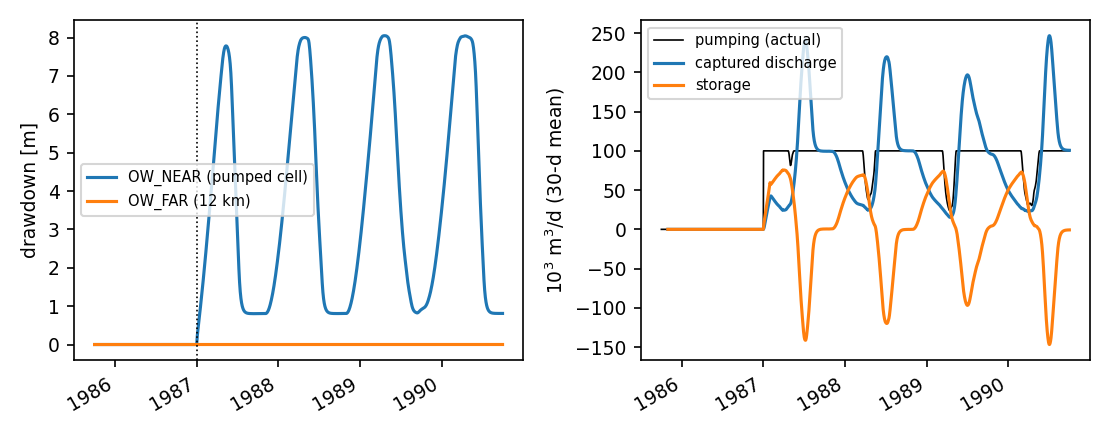
\includegraphics[width=\linewidth]{figures/fig_pumping.png}
\caption{Pumping test: drawdown at the monitoring wells (left) and where the pumped water comes from (right).}\label{fig:pumping}\end{figure}
\begin{figure}[!htbp]\centering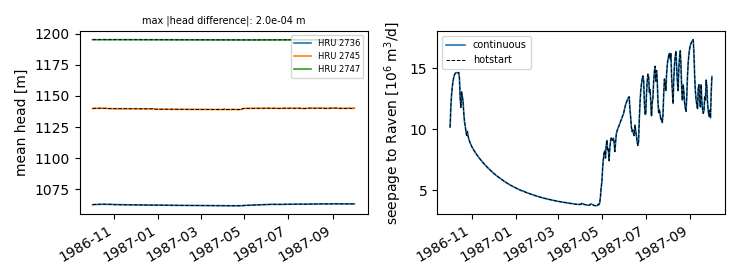
\includegraphics[width=\linewidth]{figures/fig_hotstart.png}
\caption{Restart: the second year of a continuous run (solid) and of a run restarted from \cmd{solution.rvc} (dashed).}\label{fig:hotstart}\end{figure}
\begin{figure}[!htbp]\centering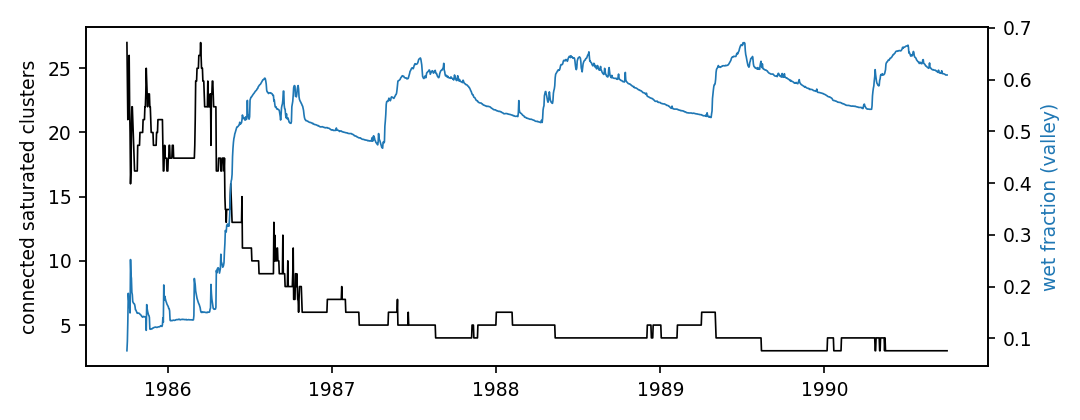
\includegraphics[width=0.9\linewidth]{figures/fig_connectivity.png}
\caption{Drying and rewetting: number of separate wet areas in the top layer (black) and wet fraction of the valley aquifer (blue).}\label{fig:conn}\end{figure}

\paragraph{Reservoirs that run dry.} In a 20-year test with a reservoir deliberately drawn empty by a minimum flow, the
reservoir's balance error is 13.7 million m$^3$: 1\,072 of its 1\,086 dry days balance exactly. Almost all of the rest
falls on the day after the reservoir empties, when the outflow still averages in the release rate at the end of the
previous day although the lake is empty. This lies in Raven's own reservoir routine, not in the coupling
(Section~\ref{ch:limits}, known issues).

\paragraph{River losses.} \cmd{tests/watershed\_balance.py} WB7--WB14 run a losing river (bed conductivity 20~m/d, the
water table 6~m deep, 40~mm/d of rain on days 1--3). A reach fed by an inflow hydrograph loses water from the inflow on
every step, and Raven's balance error stays at round-off ($3\times10^{-14}$~mm), also in a run restarted on a take day
and in each member of a 2-member ensemble. A headwater reach with a 10-day in-catchment unit hydrograph supplies its loss
from its outflow on the dry days: of 302.1~m$^3$ of leakage, 1.15~m$^3$ is still carried at the end (lost on the day the
reach stops flowing), and its outflow is 300.9~m$^3$ lower than without the river, the loss applied. With
\cmd{ROUTE\_DUMP} the reach stops flowing on day~4 and that day's 112.3~m$^3$ is carried, warned about and reported as a
run total. WB10 repeats the losing reach with every channel routing method (Muskingum and Muskingum-Cunge over 300~km,
storage coefficient, \cmd{ROUTE\_HYDROLOGIC}, diffusive wave and plug flow over 30~km), fed by an inflow that stops after
5 days: the volume leaving the watershed is lower than without the river by the loss taken (6\,539.9 against
6\,539.8~m$^3$ for Muskingum, within the file's digits) and the channel storage ends the same (the test allows
$10^{-5}$ of the loss taken, 0.065~m$^3$ for Muskingum; the run ends 0.007~m$^3$ apart), also with an irrigation demand on
the reach. WB11: a \cmd{ROUTE\_EXTERNAL} reach whose outflow a live file sets to
0.02~m$^3$/s every step delivers that outflow less the step's take (220.4~m$^3$/d), and its channel storage ends as without
the river. WB12: 2-member ensembles with \cmd{ROUTE\_HYDROLOGIC}, \cmd{ROUTE\_STORAGECOEFF} and \cmd{ROUTE\_TVD}, with and
without groundwater: every member's \cmd{Hydrographs.csv} (and \cmd{GWBudget.csv}) equals the single run's (the test
allows no difference without groundwater and $10^{-12}$ relative with it; the runs differ by 0). That member 1's
\cmd{Hydrographs.csv} and \cmd{WatershedStorage.csv} without groundwater are byte-identical to base Raven's member 1
was checked separately with base Raven for the three methods; WB12 does not run base Raven. WB13: the WB10 reach restarted with another \cmd{:TimeStep}
(0.5 then 1~d, 1 then 0.25~d) right after a take from the outflow or from the inflow, with \cmd{ROUTE\_HYDROLOGIC} and
\cmd{ROUTE\_STORAGECOEFF}: the outflow leaving the watershed over both parts is lower than without the river by the leakage
MODFLOW received (2\,980.96 against 2\,981.16~m$^3$, the file's digits), the channel storage ends the same (the test
allows $10^{-5}$ of the leakage, about 0.03~m$^3$; the runs end within $10^{-11}$~m$^3$) and Raven's balance error stays
at round-off.
WB14: the same reach with \cmd{ROUTE\_DIFFUSIVE\_WAVE}, whose inflow history Raven averages to a longer step, restarted
right after a take from the inflow, in five chains of \cmd{:TimeStep}: 0.5 then 1~d; 0.25 then 1~d; 0.25, 0.5 for half a
day, then 1~d; and two with a middle part of one step, 0.1, 0.2, 1~d and 1, 0.2, 1~d. In every part Raven's balance error
of the river run equals that of the same run without the river (the test allows $10^{-6}$~mm; the runs differ by at most
$6\times10^{-14}$~mm; the runs without the river carry Raven's own error of up to 2.2~mm in the chains with a one-step
part, Section~\ref{ch:limits}), and the leakage equals the lower outflow plus the lower channel storage at the end (the
test allows 0.5~m$^3$ plus $10^{-5}$ of the leakage; 2\,910.19 against 2\,910.11~m$^3$ for 0.5 then 1~d, the file's
digits). A restart (0.5 then 1~d) from a \cmd{solution.rvc} without \cmd{:GWRiverInflowTakes}, written by
\cmd{RAVEN\_EXE\_REF}, has no larger balance error than that build's own restart from the file (0.01742~mm in both; run
only when \cmd{RAVEN\_EXE\_REF} is set). WB14's reach is fed by a steady inflow; with takes on a reach upstream, the
restart books the takes exactly, and Raven's averaging of the downstream inflow history adds its own error (Section~\ref{ch:limits}).
\cmd{tests/boundary\_recharge.py}: an HRU over specified-head cells whose polygon reaches 0.05~m into a
neighbouring cell gives that 10~m$^2$ sliver its own share of the recharge only (399.9 of the 400~m$^3$/d go to the
specified heads; seepage to Raven 135.1 against 134.8~m$^3$/d without the sliver). The same holds for an HRU without soil under \cmd{:SoilZone PHYSICAL} (BR3: 799.8 of 800~m$^3$/d to the specified heads).

\section{Independent checks}\label{sec:independent}
\subsection{Geometry against standard libraries}
The geometry functions are compiled into a stand-alone test and compared with widely used libraries
(Table~\ref{tab:geom}); the readers of the spatial inputs are checked against the same libraries and against files
that must be refused (Table~\ref{tab:readers}).
\begin{table}[!htbp]\centering
\caption{Geometry functions against independent libraries.}\label{tab:geom}
\begin{tabularx}{\linewidth}{Y P{0.22\linewidth}P{0.2\linewidth}}\toprule\hdr
Function & Reference & Largest difference\\\midrule
Polygon clipping and area (400 random, mostly concave polygons) & shapely & $4.6\times10^{-12}$ (relative)\\
Equal-area projection (300 points over the Liard region) & pyproj (same sphere) & $6.7\times10^{-7}$ m\\
Albers and Lambert conformal conic projections (ten cases, also with the origin at either pole and with false eastings) & pyproj (PROJ) & $4.7\times10^{-7}$ m\\
Projection round trip & -- & exact\\
Bilinear raster sampling of a plane, which bilinear sampling reproduces exactly (200 points); the no-data margin of half a cell beyond the edge & the plane & $3.6\times10^{-15}$; a value 0.4 cell beyond the edge, none 0.6 cell beyond\\
\cmd{:InputCRS}: a UTM raster holding a plane, sampled at 300 lon/lat points & pyproj (PROJ) & $3\times10^{-10}$ (of values $\sim10^3$)\\
\cmd{:InputCRS}: UTM GeoJSON polygons and lines read back in lon/lat & pyproj (PROJ) & $1.1\times10^{-11}$ degrees\\\bottomrule
\end{tabularx}
\end{table}
\begin{table}[!htbp]\centering
\caption{Readers of the spatial inputs against independent libraries and reference files.}\label{tab:readers}
\begin{tabularx}{\linewidth}{Y P{0.22\linewidth}P{0.2\linewidth}}\toprule\hdr
Input & Reference & Result\\\midrule
GeoJSON and ASCII-grid variants (3-D coordinates, string IDs, holes, cell-centre headers, \dots) & shapely, reference values & read correctly\\
GeoJSON numbers (14 files): coordinates that are strings, \cmd{null}, \cmd{true} or too large; \cmd{NaN}, \cmd{Infinity}, hexadecimal numbers and leading zeros; features with and without \cmd{"properties"} & the JSON standard & the invalid ones refused, naming the feature, ring and vertex or the line and column; a feature without \cmd{"properties"} refused only where an ID is read\\
\cmd{:InputCRS}: projected \cmd{"crs"} member without \cmd{:InputCRS}, another projection, lon/lat file with \cmd{:InputCRS}, projected coordinates or raster without \cmd{:InputCRS} & -- & refused\\
\cmd{"crs"} members: EPSG:4326, 4269, 4617, 6318, 4979, 4267, a versioned URN (\cmd{EPSG:6.6:4326}), an \cmd{opengis.net} URL (4269), OGC CRS83; a versioned URN of UTM 10N; EPSG:3157 and 4647 (projections, not built in) & EPSG registry (pyproj) & geographic ones read as lon/lat (refused with \cmd{:InputCRS}); the URN read by its code; 3157 and 4647 ask for their parameters, which are then accepted\\
\cmd{"crs"} EPSG:2227 (US survey feet); a file with a UTF-8 byte-order mark; \cmd{:InputCRS} with letters or units in a parameter (\cmd{-ll7}, \cmd{O.9996}, \cmd{500km}), surplus or missing values, an unknown ellipsoid, \cmd{EPSG:32610x} & -- & 2227 refused; the file read; each specification refused, naming the parameter or value (\cmd{geomtest\_check.py})\\
GeoTIFF reader: 228 files written by GDAL and tifffile (every compression, predictor, sample type and byte order; strips and tiles, classic and BigTIFF; NODATA; internal masks; PixelIsPoint; EPSG codes; GDAL's band scale and offset, and role-less items of those names) & their ESRI ASCII twins & every value and the corner exact; the same samples bit for bit\\
ESRI ASCII grids: GDAL's \cmd{dx}/\cmd{dy} header (with corner or centre), \cmd{NODATA\_value nan}; more values than \cmd{ncols}$\times$\cmd{nrows}, a wrapped grid, fewer values, an unknown key, a value or header value that is not a number & the GeoTIFF with the same pixels; the $-9999$ twin & the same samples bit for bit; each malformed grid refused with its reason\\
GeoTIFF reader: 34 unsupported or damaged files (also a prime meridian given only by its longitude or by the datum, a projected code in feet without its units key, a band unit in feet), an oversized file, and damaged copies of every fixture (bytes changed, cut, inserted, random) & -- & each refused with its reason; no crash (also under AddressSanitizer)\\\bottomrule
\end{tabularx}
\end{table}

\paragraph{GeoTIFF rasters.} \cmd{tests/geotiff/geotiff\_check.py} reads 228 GeoTIFF files written by GDAL and tifffile
(every supported compression, predictor, sample type and byte order, in strips and tiles, classic and BigTIFF, with
NODATA values, internal masks, \cmd{PixelIsPoint} and several EPSG codes) and compares each with an ESRI ASCII twin holding the same
values: the corner, cell size and every value agree exactly, and Raven's sampling of the two at 4\,000 points agrees bit for
bit; rasters with rectangular pixels agree with an independent bilinear sampler. Each of 186 of these files used as \cmd{:LandSurface} of a small model, and 43 as \cmd{:BedrockSurface}, gives outputs
byte-identical to its twin (the model files hold the sampled cell elevations); so do projected rasters under
\cmd{:InputCRS}. Unsupported, damaged and oversized files, a code that disagrees with \cmd{:InputCRS}, and a DEM or bedrock
raster that covers no active column stop the run with their reason; a raster covering part of the columns gives a warning
with their number. Damaged copies of every file (bytes changed, cut or inserted, random content) are refused with a message
or read, never crash the reader (also checked once under AddressSanitizer and UndefinedBehaviorSanitizer).

\paragraph{Projected input files.} The Liard example with every geometry and raster input converted to UTM zone 10
(\cmd{tests/crs\_inputs.py}, PROJ through pyproj, \cmd{:InputCRS EPSG:32610}) gives the same grid as the example in
longitude/latitude: the same active columns and cells, river, boundary and well cells, polygon areas within
$8\times10^{-12}$ and HRU--cell overlaps within $1.1\times10^{-9}$ of a cell; without rasters the hydrographs agree to the
printed digits and the groundwater budget within $2\times10^{-8}$ over 120 days. With the DEM and bedrock resampled to
300~m UTM grids the model top differs by 0.018~m on average (the resampling) and the hydrographs by $10^{-3}$. Projected
files without \cmd{:InputCRS}, files in another projection and wells given by \cmd{X} and \cmd{Y} without \cmd{:InputCRS}
stop the run with a message naming \cmd{:InputCRS}; with \cmd{:InputCRS}, a DEM, a bedrock raster, the HRU polygons or a
boundary line left in longitude/latitude stop the run as ``looks like longitude/latitude''. The boundaries of this test have
heads above their cells (the general-head line by its \cmd{HEAD}, the specified-head lake by a \cmd{:BoundaryHead} series
with \cmd{HEAD 0}), and both runs give them the same cells (3 and 9).

\paragraph{A layer that starts dry.} The start-up warning for a layer that starts dry (\cmd{tests/dry\_start.py}) names
layer~2 of the Liard model with \cmd{INITIAL\_HEAD\_DEPTH} 25~m (2\,794 cells), and is absent with a steady-state start
and for the example as shipped, whose outputs equal those of the reference build.

\paragraph{Budget file and particle tracking.} With \cmd{:WriteGWBudgetFile} (\cmd{tests/budget\_file.py}, the Liard
example with a pumping well) MODFLOW's budget file holds \cmd{FLOW-JA-FACE}, the specific discharge, the saturation and
every package at every step, and its package totals equal \cmd{GWBudget.csv} within $4\times10^{-10}$; \cmd{gwf.porosity}
holds each cell's class porosity. The solution is the same with and without the option, and without it the \cmd{mf6}
folder equals the reference build's. \cmd{tools/make\_prt.py} runs MODFLOW~6 PRT on these files through the library:
eight particles around the well, tracked forward and backward, move in opposite directions; with a steady-state first
period each is released once, at the start (forward) or end (backward) of Raven's run, and ends within it. With flows
saved every fifth step only (\cmd{:HeadSaveFrequency 5}) the script stops, in both directions, with a message naming
\cmd{:HeadSaveFrequency 1}.

\subsection{Exchanged flows against MODFLOW's own budget}
MODFLOW writes its own volume budget in its list file. For runs covering every package, every flow the coupling exchanged
is compared with MODFLOW's figure for the same step, read by package name (\cmd{tests/budget\_xcheck.py};
Table~\ref{tab:listcheck}); the differences are at the printing precision of the list file. The check fails when it
compares nothing.
\begin{table}[!htbp]\centering
\caption{Coupler flows against MODFLOW's list-file budget.}\label{tab:listcheck}
\begin{tabularx}{\linewidth}{P{0.25\linewidth}Y P{0.2\linewidth}}\toprule\hdr
Run & Packages compared & Largest difference\\\midrule
20-year Liard & recharge, drains, rivers, storage & $6.2\times10^{-7}$\\
Pumping and boundaries & + wells, general-head boundaries & $6.9\times10^{-7}$\\
Fixed head and delay & + fixed heads & $6.1\times10^{-8}$\\
Wetland exchange & + store exchange & $1.1\times10^{-7}$\\
Reservoir & + reservoir seepage & $2.6\times10^{-7}$\\
Drying & + water-table ET & $4.1\times10^{-8}$\\\bottomrule
\end{tabularx}
\end{table}

\subsection{Grid size and time step}
The accounts stay exact for any cell size and time step (Table~\ref{tab:invariance}; subbasin 52, one year). The first
rows use a head tolerance of 0.01~m; with it the worst single step on 4~km cells is 0.47\% of the flow, and the default
tolerance of 0.00001~m brings it down to 0.002\%. Raven's balance stays at its first step's value on every step (base
Raven's for this model: 0.431~mm with daily steps, 0.216~mm with half-day steps).
\begin{table}[!htbp]\centering
\caption{Invariance to cell size and time step.}\label{tab:invariance}
\begin{tabular}{lrlrr}\toprule\hdr
Set-up & Active columns & Recharge & Worst step & Raven balance\\\midrule
1 km cells & 2\,147 & exact & 0.029\% & 0.431 mm\\
2 km cells & 545 & exact & 0.092\% & 0.431 mm\\
4 km cells & 142 & exact & 0.47\% & 0.431 mm\\
4 km cells, default tolerance & 142 & exact & 0.002\% & 0.431 mm\\
2 km cells, half-day steps & 545 & exact & 0.059\% & 0.216 mm\\\bottomrule
\end{tabular}
\end{table}

\section{Model files and faulty input}\label{sec:mf6files}
Raven writes every MODFLOW input file, and \cmd{grid\_cells.geojson}, before it loads the MODFLOW library; in the
existing-model mode it also copies the model and prepares the simulation, time and name files first. Almost everything
except the solve itself can therefore be checked without MODFLOW, by pointing \cmd{RAVEN\_MF6\_LIB} at a file that does not
exist: the run then stops, with a message, just after the files are written. The checks of this section use this, and
run again with the library where it matters.

\paragraph{MODFLOW input files.} \cmd{tests/mf6files\_check.py} builds 16 set-ups over every grid type, rotation,
refinement, layers by elevation, aquicludes, boundaries, wells, lakes and imported cells, and checks the files Raven
writes: FloPy reads every model; cells are valid and do not overlap; the grid origin and rotation agree with the cell file
(0.5~m); DISV and DISU vertices are right; DISU connections are symmetric; face angles agree with the vertices
(1\textdegree); no vertical connection passes through an aquiclude; drains lie inside the top cell; boundary polygons
select the right cells. All 127 checks pass.

\paragraph{Faulty and unusual input.} Thirty-nine faulty or unusual set-ups of the Liard model check the messages
(Table~\ref{tab:faulty}): every error stops the run with a message that names the problem --- no crash --- and every
tolerated case runs. \cmd{tests/edge.py} adds 36 generated-model and 17 existing-model set-ups, judged without and with
MODFLOW; the valid existing-model preparations are checked in detail (stress periods split at the start date, restart
renumbering, the original model untouched). All 53 behave as required.
\begin{table}[!htbp]\centering
\caption{Response to faulty or unusual input.}\label{tab:faulty}
\begin{tabularx}{\linewidth}{Y P{0.4\linewidth}}\toprule\hdr
Input & Response\\\midrule
Missing HRU file or ID field; unknown profile or class; malformed class row & stops; names the file, field, profile or row\\
Aquiclude as top layer; zero layer thickness; value out of range ($K\le0$, $S_y>1$, negative delay, \dots) & stops; names the parameter\\
Process draining \cmd{GROUNDWATER} in a coupled HRU; no process feeding it & stops; names the process and HRU\\
Wrong library path; missing raster; well outside the model & stops; names the path, file or well\\
DEM or bedrock raster that covers no active column (another area, a wrong corner, NODATA only) / covers part of them & stops with both extents / warns with the count\\
Duplicate IDs or names; two exchanges on one store; boundary without \cmd{HEAD} & stops; names the item\\
Malformed groundwater command in \cmd{.rvg}, \cmd{.rvt} or \cmd{.rvc} & stops; names the command\\
Hotstart heads for a different grid; cells larger than the HRUs & stops; explains the mismatch\\
Monitoring well outside the model; unknown \cmd{.rvg} command & runs with a warning\\
\cmd{TO\_BEDROCK} in a middle layer; no DEM or bedrock map; coupling switched off & runs as documented\\
Malformed numbers in the \cmd{.rvg} (\cmd{:GridCellSize 2,000.0}, \cmd{2km}, \cmd{HEAD H1146}, \cmd{1146.85m}, \cmd{50.5} iterations, a \cmd{:Wells} value); a cell size giving more than $5\times10^6$ cells per layer (\cmd{:GridCellSize 50} and \cmd{60} on Liard), a refinement size giving more on a regular grid (counted with its 2:1 smoothing: 60 short lines on 400~$\times$~300~km, N24) or, by its estimate, on a quadtree grid (\cmd{:GridRefinement RIVERS 0.1}) & stops before the grid is built; names the command and the value or the estimated cells per layer (\cmd{tests/input\_checks.py})\\
A quadtree grid within the limit that needs more memory than there is (\cmd{RIVERS 0.5} on Liard, about $4.6\times10^6$ cells per layer, under a 3~GB limit) & stops naming \cmd{:GridRefinement} and the estimated cells per layer (no crash)\\
Overlapping and adjacent refinement features: 200 copies of one line (\cmd{LINES 0.1}) and 20 adjacent squares (\cmd{POLYGONS 0.5}) on a 4-HRU strip & built (the estimate counts each square once)\\
An HRU mesh of 4 HRUs of 5~$\times$~5~km with 500~m cells and one short refinement line of 0.1~m (N17) and of 2~m (N18) & N17 stops before the mesh is built (``too slow to build''); N18 is built within 120~s (65\,484 cells per layer)\\
Boundary polygons that overlap: two features, the same feature twice, a MultiPolygon of two overlapping parts (N19) & each selects the cells of the union (as the larger polygon alone)\\
Malformed numbers in the \cmd{.rvp} aquifer tables: \cmd{K\_HORIZ 1O}, \cmd{SPEC\_YIELD O.2}, a thickness \cmd{3m}, a profile parameter \cmd{2.O} (N20--N23) & stops; names the table, the row and the token\\
Malformed numbers in the \cmd{.rvc}: \cmd{:InitialGWHeads ELEVATION 98,5}, \cmd{H98.5} or \cmd{0x62}, \cmd{:InitialGWHeads FROM\_PROFILE 0}, a \cmd{:GWHeads} value \cmd{98.5x} & stops; names the command and the token (\cmd{test\_inputs.py} I22)\\
\cmd{:WellFlowRate} in \cmd{m3/s} or \cmd{L/s}; other units of a well or head series & converted to m$^3$/d (5\,000 m$^3$/d either way); stops\\
A package of an existing model named like one of Raven's (\cmd{DRN\_RAVEN}); a recharge package so named and taken over & stops with Raven's message; runs\\\bottomrule
\end{tabularx}
\end{table}

\section{Randomized testing}\label{sec:fuzz}
A test driver (\cmd{tests/fuzz\_grids.py}) builds random but valid set-ups of the subbasin-52 model, drawing every option
at random: grid type (regular, rotated and refined, quadtree, HRU mesh, imported cells, layers by elevation), rotation,
refinement and XT3D, cell size (1--3 km), minimum coverage, one-day or half-day steps, conductivities, initial depth,
seepage leakance and smoothing, water-table ET, recharge delay, steady-state start, wetland exchange, 0--2 pumping wells,
monitoring wells, a general-head boundary, a fixed-head area and a coupled reservoir. Every run is checked independently of
the audit tool: exact recharge, seepage, river, store and reservoir identities; MODFLOW's balance (every converged step
below 0.1\%, cumulative below $10^{-4}$); Raven's balance below 1 mm; agreement with MODFLOW's list file; and, for about a
third of the set-ups, a restart that must reproduce the continuous run (every flow within $10^{-4}$ of its largest value in
the run).

With MODFLOW 6.8.1, three batches of 24 (72 set-ups: 10 regular, 11 rotated and refined, 16 quadtree, 15 HRU mesh,
6 imported, 14 with layers connected by elevation; 49 with a reservoir; 20 with a restart comparison, largest deviation
$3.1\times10^{-6}$) and two batches of 12 that always have a reservoir and lake refinement (24 set-ups, 6 with a restart) all
pass every check, including MODFLOW's list-file budget and the reservoir identity. The optional fully implicit XT3D can
fail to converge where cells dry and rewet (in one random set-up on 38 of 45 days, with exact accounts on the converged
days and the safeguard limiting the exchange on the others); it is therefore off by default.

\section{Grid types}\label{sec:vgrids}
\begin{plain}
Every kind of grid is checked in four ways: its cells cover the area exactly with no gaps or overlaps; two different ways of
handing the same cells to MODFLOW give the same answer; the answer matches an exact textbook solution and gets closer to it
as the cells get smaller; and a restarted run matches a continuous one.
\end{plain}
Every grid option is verified the same way as the default grid, plus the checks below.

\paragraph{Geometry of the grids.} A stand-alone test (\cmd{tests/gridtest.cpp}) checks every generator: cells tile the
domain exactly (area sums equal to $10^{-15}$), neighbours are symmetric, each cell's perimeter equals its shared faces plus
the domain edge, Voronoi connections are exactly orthogonal, quadtree neighbours differ by one level at most, clipping
handles concave cells and lattices of cocircular seeds, and grids survive the linkage cache bit for bit. It also checks
that the grid-size stop names its cause (the cell size, a refinement, the seeds of an HRU mesh, an imported grid or an
existing model).

\paragraph{Two formats, one answer.} The quadtree cells were run once as DISV (MODFLOW computes the geometry) and once
imported as DISU (the coupler computes connection lengths, face widths and directions): all flows agree to $6\times10^{-7}$ and
water tables to 0.3 mm. A regular grid written as DISU gives heads identical to DIS. Solving the coupler's DISU equations
independently in Python reproduces MODFLOW's heads to $3\times10^{-8}$ m.

\paragraph{Analytical solution.} A textbook case has an exact answer to compare with: a single well pumping from an aquifer
whose water level is held fixed all around, far away (the \emph{Thiem} solution). Close to the well the water level falls in
a known way with distance. A well pumping 5\,000 m$^3$/d from a confined aquifer ($T=500$ m$^2$/d) inside a
20 km square with fixed heads on its edge should give the Thiem profile $h=A+\frac{Q}{2\pi T}\ln r$. The slope fitted to
all cells between four cell sizes and 3 km from the well is compared with $Q/(2\pi T)$ in Table~\ref{tab:thiem}: every grid
converges to the analytical value as its cells shrink, and the solutions are symmetric around the well (slopes in the four
directions within 0.6\%).

\begin{table}[!htbp]\centering
\caption{Thiem test: error of the fitted slope $\partial h/\partial\ln r$ (\cmd{tests/thiem}, MODFLOW 6.8.1; every run
checked, none with a failed step).}\label{tab:thiem}
\begin{tabular}{lrrr}\toprule\hdr
Grid & Coarse & Medium & Fine\\\midrule
Regular, 500 / 250 / 125 m & +0.60\% & +0.04\% & +0.01\%\\
Regular 250 m, rotated 17\textdegree & & +0.03\% & \\
Regular 1 km refined to 125 m at the wells & & +1.01\% & \\
Quadtree, base 1\,000 / 500 / 250 m, 62.5 m at the wells & +0.80\% & +0.59\% & +0.26\%\\
Imported cells (the 250 m quadtree) & & & +0.25\%\\
HRU mesh, 500 / 250 m (250 m with XT3D) & +0.57\% & +0.29\% & $-$0.06\%\\\bottomrule
\end{tabular}
\end{table}

\paragraph{Lakes.} A reservoir with seepage to the aquifer was placed on the largest coupled HRU of subbasin~52 and each
refinable grid (3~km cells) was refined around it with \cmd{LAKES} (\cmd{tests/lake\_test.py}). The median size of the
cells touching the lake falls from 3\,000 to 750~m (rotated regular grid), from 3\,000 to 375~m (quadtree) and from 1\,210 to
490~m (HRU mesh); a \cmd{POLYGONS} file with the same outline gives the same mesh. The water accounts stay exact (MODFLOW
residual below $1.2\times10^{-11}$), and the reservoir's seepage reaches MODFLOW exactly one step after it leaves the lake
(sent $=$ previous step's volume in transit to $1.6\times10^{-10}$; delivered $=$ sent); MODFLOW's own list-file budget shows
the same reservoir seepage.

\paragraph{Restarts.} For every grid type a 60-day run is compared with a 30-day run restarted from its
\cmd{solution.rvc} (\cmd{tests/restart\_test.py}: subbasin-52 model with 3~km cells, a pumping well and half-day steps):
regular $9.9\times10^{-7}$, rotated and refined $1.9\times10^{-7}$, quadtree $4.4\times10^{-7}$, HRU mesh $1.9\times10^{-7}$,
layers by elevation $8.3\times10^{-8}$, with exact water accounting in all.

\paragraph{Randomized testing.} The randomized set-ups of Section~\ref{sec:fuzz} draw the grid type at random; their
restart criterion scales each day's difference by the flow's largest value in the run, as the existing-model tests do.

\section{Coupling an existing model}\label{sec:vexisting}
\begin{plain}
The existing-model mode is tested on a MODFLOW model built independently of Raven. It is also tested on a copy of that
model in feet and seconds, which must give the same answers; on a model that Raven built itself and then read back in, which
must reproduce Raven's own run; with restarts; with deliberately wrong input, which must be caught; with random set-ups;
and with two models of the USGS example collection. In every run no water is created or lost.
\end{plain}
The existing-model mode is tested on the synthetic Liard model of Chapter~\ref{ch:existing} (a rotated UTM grid, four
layers, monthly stress periods, wells, rivers and a head boundary), built independently of Raven
(\cmd{tests/existing/make\_ext\_model.py}), and on a feet/seconds copy of it. Every run keeps the water accounts exact:
Raven's recharge reaches MODFLOW exactly, the MODFLOW residual including the model's own packages is about
$2\times10^{-11}$, seepage and river exchange balance to $10^{-11}$, and no step fails.

\begin{table}[!htbp]\centering
\caption{Existing-model mode: tests and results.}\label{tab:vexisting}
\begin{tabularx}{\linewidth}{P{0.42\linewidth}Y}\toprule\hdr
Test & Result\\\midrule
Built-in projections against PROJ (9 systems, 18\,000 points) & largest difference 3 micrometres\\
Cell outlines from MODFLOW (\cmd{:MF6CRS}) against a cell file & recharge identical; other flows within $3.5\times10^{-7}$\\
Feet and seconds against metres and days & recharge identical; other flows within $4.6\times10^{-6}$\\
Round trip: a Raven-generated model re-imported & recharge identical; outlet flow within $1.7\times10^{-6}$\\
\cmd{:OverlapWeights} (computed in UTM) against cell outlines & recharge identical; seepage within $4.5\times10^{-7}$, rivers within $4\times10^{-6}$\\
Restarts (inside a stress period; before a change of well rates) & within $1.4\times10^{-7}$; the renumbered well data switch on the right date\\
Water-table ET, surface-store and reservoir exchange (\cmd{EVT\_RAVEN}, \cmd{SWX\_RAVEN}, \cmd{RES\_RAVEN}), metres/days and feet/seconds, 120 days (\cmd{tests/existing/ext\_exchanges.py}) & accounts exact (MODFLOW residual below $4\times10^{-11}$); each package's flows in MODFLOW's budget file and list file equal \cmd{GWBudget.csv} (within $4\times10^{-10}$; the list file to its printed digits); water-table ET at most 5\% of the unmet PET on any day; feet/seconds: the exchanged flows within $10^{-7}$, the other columns within $2\times10^{-5}$ (one step of 120 days; the two models are solved separately to the same tolerance); a restart with reservoir seepage in transit within $3\times10^{-7}$; a kept EVT package with \cmd{EXTINCTION\_DEPTH} refused\\
Later starts (\cmd{ext\_inputs.py}, \cmd{restart\_ext.py}): TDIS and water-mover rows in \cmd{OPEN/CLOSE} files; wells driven by a TS6 series, restarted between two of its entries; 6-hour steps restarted at 12:00; DIS6 and STO6 under names of their own in the name file & identical to the runs with the rows inline; within $4.2\times10^{-7}$ and $2.3\times10^{-6}$ of the continuous runs; \cmd{TAS6} refused; the renamed packages read (\cmd{GWBudget.csv} identical to the usual names', MODFLOW's storage flows kept)\\
Dry and specified-head cells under the exchanges (\cmd{ext\_exchanges.py}): water-table ET in a model without \cmd{NEWTON} whose top cells dry (MODFLOW moves the ET to the cell below); a reservoir over cells that become specified heads (all, or 2 of 5); a reservoir over dry cells without \cmd{NEWTON} & water-table ET equal to MODFLOW's budget file on every saved step, MODFLOW error $5\times10^{-3}$~m$^3$/d on $6\times10^{5}$~m$^3$/d; the reservoir books exact (sent = delivered $-$ gain not supplied $+$ not delivered), seepage not delivered $6.4\times10^{5}$~m$^3$ returned and its run total equal to its column, all of it delivered when 3 of 5 cells remain; no HDRY or NaN in the outputs\\
Safeguards (14 faulty set-ups, \cmd{guards.py}) & every one stops with a message naming the problem\\
Randomized set-ups (units, link, stream mapping, seepage, ET kept or taken over, coverage, restarts; \cmd{fuzz\_ext.py}); checked with the audit identities and MODFLOW's own budget file & 20 of 20 pass, 6 with a restart (within $2.7\times10^{-7}$); MODFLOW's saved flows of Raven's packages agree to $10^{-10}$\\
Sanitizers (AddressSanitizer, UndefinedBehaviorSanitizer) on the coupling's code: both units, all three links, seepage off, restarts & no error\\\bottomrule
\end{tabularx}
\end{table}
The test model allows 300 outer iterations. Its metres/days version needs 288 of them in its first (steady-state)
period, and the feet/seconds version a few more, so one feet/seconds set-up does not converge on that step while its twin
does; every later step takes the same number of iterations in both, and with 500 iterations both converge on every step.
The weights test shows why the overlaps are normalised per HRU: the weights were computed in the model's projection, whose
areas differ from Raven's by about 0.5\% at this latitude, and the recharge volumes still agree exactly. In the two-year
example the stream package loses about 3.8 million m$^3$/d to the aquifer; the small headwater reaches cannot always supply
their share, so up to 106 million m$^3$ of river loss is carried from step to step at times --- all of it supplied by the end
of the run, as the accounting requires.

\subsection{USGS example models}\label{sec:usgs}
Two models of the USGS MODFLOW~6 example collection (\cmd{mf6examples.zip}) are coupled as existing models with
\cmd{:OverlapWeights}. They are not georeferenced, so the Liard HRUs of subbasin~52 are laid over each model's active cells,
with \cmd{.rvh} areas equal to their zones so that Raven's recharge depths become the same depths on the model
(\cmd{tests/existing/usgs\_sagehen.py}, \cmd{usgs\_capture.py}).

\paragraph{Sagehen Creek} (a real watershed in the Sierra Nevada: 73$\times$81 cells of 90~m, one convertible layer,
Newton, a steady-state day and 398 daily periods, an unsaturated-zone package (UZF) whose rejected infiltration and
groundwater discharge the water mover (MVR) sends to streams (SFR), land-surface drains also moved to SFR, three specified
heads). Raven takes over the UZF package, so its recharge replaces the model's infiltration, and removes the 3\,375 movers
that name it from the working copy. The recharge identity, the river bookkeeping and the seepage returned are exact in every
case; the water the model's packages pass to the mover is part of MODFLOW's balance. MODFLOW's cumulative residual is
$8.5\times10^{-7}$ with the model's own loose solver (\cmd{OUTER\_DVCLOSE} 0.03~m, \cmd{INNER\_RCLOSE} 1\,000~m$^3$/d),
$2.8\times10^{-10}$ with a tight solver, and $1.3\times10^{-11}$ with Raven's seepage drains beside the model's own. A
restart at day~200, inside the daily periods (the mover renumbered), reproduces the continuous run to $3.3\times10^{-8}$.
Keeping the UZF package beside Raven's recharge (recharge counted twice, the user's choice) runs with exact accounts; one
day of the snowmelt peak misses the tight tolerance and is flagged. The drains as Raven's stream package are refused,
because the mover already sends their water to SFR.

\paragraph{Stream capture} (a steady-state model: 40$\times$20 cells of 250~m, time in seconds, one stress period of one
second, a river, six pumping wells, specified heads). Raven recognises the steady-state model and stretches its period over
the 60-day run, so each day is a steady-state solution; the storage column stays zero. The river carries its exchange to
Raven's reaches (subbasin of the dominant HRU); recharge identity and river bookkeeping are exact, MODFLOW's residual is
$2.8\times10^{-9}$, and a restart at day~30 reproduces the continuous run to $1.0\times10^{-7}$. With the model's own
tolerance of $10^{-8}$~m and 100 outer iterations, four days do not converge; they are flagged and the accounts on the
other days are exact. The Liard seepage leakance of 1/d lets the water table of this thin, flat-topped aquifer reach the land
surface on the wettest days, where MODFLOW's Newton solver does not converge on two of them; 0.01/d, suited to its
conductivity of about $7\times10^{-5}$~m/s, converges every day.

\subsection{MODFLOW versions}\label{sec:mf6versions}
Every test of \cmd{tests/run\_all.py} has been run with MODFLOW~6.8.1 and~6.6.3. Raven writes the \cmd{NEWTON} option
without its \cmd{UNDER\_RELAXATION} keyword (Section~\ref{ch:mf6}): with that keyword MODFLOW~6.6.3 resets a head that falls
below the cell bottom, the Newton change of a drying thin aquitard cell repeats unchanged at every iteration, and the default
Liard grid fails to converge on 295 of 344 days. Without it, every step passes with both versions with the same numbers: the
Liard grid table agrees to the last digit shown. For existing models Raven reads the library's version and warns when a model
uses the keyword with a version before~6.8.

% Verification of the soil zone (tests/soilzone): test models, the column and the hillslope, the water table in every
% position, the interface and MODFLOW's side, the unsaturated-zone methods, inputs and robustness.
\section{The soil zone}\label{sec:vsoilzone}
The soil-zone coupling (Section~\ref{ch:soilzone}) is tested at three levels: the unsaturated column and the capillary rise
relation on their own against independent solutions; small coupled models that put the water table in each of the
positions of Figure~\ref{fig:szregimes}; and the same models coupled again as existing MODFLOW models. The tests in
\cmd{tests/soilzone} build small synthetic models (\cmd{sz\_models.py}: a generated MODFLOW model under Raven HRUs with
soil, forcing written by the script) and compare them with exact values or with a MODFLOW-only reference in which the soil
zone is a MODFLOW layer and a drain at the land surface takes the overflow (\cmd{sz\_reference.py}); only LP1 starts from the
Liard example. Every coupled run is also checked by \cmd{sz\_check.py}, which closes, step by step, MODFLOW's balance,
Raven's balance and the recharge, soil-zone and unsaturated-zone identities of Section~\ref{sec:accsz} at their standard
limits (recharge $5\times10^{-9}$, soil zone and columns $10^{-8}$ relative, from the first step; \cmd{sz\_check.ID\_LIMITS}),
and requires no soil-zone shortfall. Its self-test shows that the column identity catches a small leak: exact books give 0,
and a leak of $10^{-4}$~m$^3$ per step on a 9\,776~m$^3$ store gives $2.4\times10^{-7}$ and fails. The numbers below are those
of the full mode of \cmd{tests/run\_all.py} with MODFLOW~6.8.1, except where a table says otherwise.

\subsection{The column, the hillslope and the interface}\label{sec:vszbasic}
\begin{longtable}{P{0.13\linewidth}P{0.42\linewidth}P{0.36\linewidth}}
\caption{The column, the hillslope, time steps, restarts and the Liard model (\cmd{soilzone\_unit}, \cmd{spike\_xmi},
\cmd{test\_column}, \cmd{test\_hillslope}, \cmd{test\_dynamics}, \cmd{test\_restart}, \cmd{test\_liard\_physical}).}\label{tab:vszbasic}\\
\toprule\hdr Test & What is checked & Result\\\midrule\endfirsthead
\caption[]{The column, the hillslope and the interface (continued).}\\
\toprule\hdr Test & What is checked & Result\\\midrule\endhead
Unit & \cmd{soilzone\_unit.cpp}: filling and draining of the layers, the sub-grid level and its inverse, the contact weights and flux derivatives against finite differences, continuity across the sample bases, the local solve (monotone, root, mass), the Robin slope; 20\,000 random cases each & 57 checks, 0 failed\\
XMI & \cmd{spike\_xmi.py}: values written between MODFLOW's outer iterations through XMI (GHB \cmd{BHEAD}/\cmd{COND}, RCH \cmd{RECHARGE}) reach the solver; the coefficients are recomputed every outer iteration; a solve after convergence is a normal iteration & all three hold (MODFLOW 6.8.1)\\
CT1 flat column & closed column, $S_y$ = drainable porosity = 0.2, recharge 10~mm/d: the water table rises 50~mm/d below the soil base and inside the soil; water table and soil level agree once connected; the soil zone (400~mm of capacity) is full on day~41 & rise 49.95~mm/d below and inside; largest difference $1.3\times10^{-4}$~m; full on day 41\\
CT1b & the same with $S_y=0.08$: 125~mm/d below the base, 50~mm/d inside, storage-consistency warning & 124.7 and 49.95~mm/d; warning given\\
HS1 hillslope, wetting & ten 100~m HRUs on a 0.5\,\% slope over a closed 20~m aquifer, rain 10~mm/d for 150 days (Figure~\ref{fig:szhillslope}): against the MODFLOW-only reference & heads within 3.3~cm (mean 0.67~cm), soil level within 3.9~cm, total outflow within $2.5\times10^{-5}$; overflow begins on day 16 in both; the toe connects first (day 7), HRU 2 last (day 73), HRU 1 never\\
HS2 hillslope, drying & the 150 dry days that follow: HRUs that connected and whose reference head ends below their base lose their saturation; those whose head stays above it stay saturated; no overflow where the water table is below the land; the upslope overflow stops with the rain; the toe's seepage recedes; \cmd{-{}-selftest} shows that each check fails on altered results & HRUs 2--7: $F=0$ at the end; 8--10: $F=1$; upslope overflow ends on day 150; toe 814~m$^3$/d on day 161, 173.5 on day 300 (reference 173.6); saturated HRUs 9 $\to$ 3; each of the four self-test mutations fails\\
DY1 time step & the hillslope with steps of 1~d, 6~h and 1~h, each against the reference with the same step: the splitting error of Raven's processes ahead of the exchange shrinks with the step & mean head difference 0.67, 0.24 and 0.14~cm; outflow within $6\times10^{-5}$\\
DY2 stiff contact & a thin, conductive soil--aquifer contact ($\dt/t_c\approx48$ for daily steps): the iterated interface against one explicit pass & iterated: at most 9 updates, heads within 4.2~cm of the reference, outflow $8\times10^{-5}$; one pass: 0.99~m and 1.3\,\%\\
SG sub-grid & \cmd{:SoilZoneSubgrid 5} on the same slope: the saturated fraction changes smoothly instead of cell by cell & largest daily change of $F$ 0.42 (1.0 with one point per cell); outflow within 0.4\,\% of the one-point run\\
Restart & RS1: 300 days against 150 + 150 days from \cmd{solution.rvc} (\cmd{:GWSoilZoneColumns}); RS2: an existing model with a specified-head toe and unsaturated columns, 10 days against 5 + 5; RS3: no \cmd{:SoilZone PHYSICAL}, seepage holding the lowest soil layer above capacity, 30 days against 12 + 18; RS4: \cmd{KINEMATIC} and \cmd{LAG} with $S_y$ equal to the porosity, 20 days against 10 + 10; RS5: a coupled restart continues exactly, \cmd{RICHARDS} columns with a reservoir, a specified head, negative recharge and a rising water table, \cmd{CONCEPTUAL} with every exchange, 8 days against 4 + 4, and \cmd{LAGGED} exchange with negative recharge under a \cmd{:BoundaryHead} series that holds the outlet column on some days and switches every cell off on others, restarted on days 3, 4 and 6 (off to held, held to off, off to held); RS6: a lagged-exchange debt open at a restart, 2 days then restarted with \cmd{LAGGED}, \cmd{AFTER} and without \cmd{:SoilZone PHYSICAL} & 1\,500 rows: water table and soil level $2\times10^{-10}$, $F$ $1.2\times10^{-7}$, exchange $2.4\times10^{-6}$ (limit $10^{-4}$); RS2 $2.5\times10^{-7}$; RS3 soil storage identical, recharge and seepage within $3.4\times10^{-9}$; RS4 column storage as written, restart identical to the continuous run; RS5 every column of \cmd{GWBudget.csv}, \cmd{GWHRUState.csv} and the stores of \cmd{WatershedStorage.csv} identical (limit $10^{-9}$); RS6 the debt open after 2 days (1.594~m$^3$) reported, repaid in the first step of a \cmd{LAGGED} restart, warned about and reported as unrepaid by an \cmd{AFTER} and a \cmd{CONCEPTUAL} restart\\
LP1 Liard & the Liard example with \cmd{:SoilZone PHYSICAL SOIL[0] SOIL[1]} (85 coupled HRUs, 2~km grid, one year from 1985-10-01; soils of drainable porosity 0.02 against $S_y=0.25$, a stiff interface, storage warning expected) & 365 steps, 0 unconverged (MODFLOW and interface), 3\,509 outer iterations (at most 72 in a step), residual $8\times10^{-12}$ of the gross flow, no shortfall; 80 of 85 HRUs more than 20\,\% saturated at some time\\\bottomrule
\end{longtable}
\noindent The soil zone with existing models is verified by X1--X9 (Table~\ref{tab:vszpositions}) and by the
existing-model cases of the rough-terrain suite (Section~\ref{sec:vrough}).

\subsection{The unsaturated column and capillary rise}\label{sec:vszcolumn}
\begin{longtable}{P{0.13\linewidth}P{0.42\linewidth}P{0.36\linewidth}}
\caption{The Richards column and the rise relation on their own (\cmd{vadose\_unit.cpp}, \cmd{vadose\_ref.py}).}\label{tab:vszcolumn}\\
\toprule\hdr Test & What is checked & Result\\\midrule\endfirsthead
\toprule\hdr Test & What is checked & Result\\\midrule\endhead
Retention & $\partial\theta/\partial\psi$ and $\partial K/\partial\psi$ against finite differences, inverse, continuity at the Hutson--Cass junction & exact to $10^{-4}$ relative\\
Steady infiltration & 3~m column at 0.02 m/d against an RK4 integration of the steady profile & bottom flux = top flux to $10^{-6}$; profile within 2~cm\\
Mass & 200 days of storms beyond $K_s$ (rejection) & inflow $-$ outflow $-$ storage change $<10^{-10}$~m\\
Perched water & permeable layer over a layer 500 times less permeable & saturated zone above the contact; steady flux = accepted inflow\\
Moving water table & rising, falling, rising past the base & storage relative to equilibrium = absorbed + remaining to $10^{-12}$\\
Drainage & wet 4~m column against a 400-cell method-of-lines solution (scipy BDF), Figure~\ref{fig:szdrainage} & total 0.18\%; largest step mean 10.5\% of the peak at $\epsilon=0.02$ (1.9\% at 0.005)\\
Rise relation & (\ref{eq:rise}) against scipy quadrature; table against the direct solution over $10^{-2}\le\Delta z/\psi_a\le200$, $1.5\le b\le12$ & $10^{-3}$; table within 2.5\% (mostly 0.5\%)\\
Richards check of the rise & finite-volume column driven at $-q(d,\psi_s)$ until steady & top suction equals $\psi_s$ within 3\%\\
Speed & 4\,300 columns of 16 nodes, 10 days with a pulse & 0.2~s per day (unoptimized build)\\
Robustness & remap across materials, air-dry columns, inflow far above $K_s$, substep limit, upward demand beyond supply; randomized stress of 40\,000 column-steps & no lock-up or pressure runaway; air-dry column takes water; mass exact to $10^{-14}$\\\bottomrule
\end{longtable}

\subsection{The water table in every position}\label{sec:vszpositions}
\begin{longtable}{P{0.13\linewidth}P{0.42\linewidth}P{0.36\linewidth}}
\caption{The water table in every position, and the soil zone with existing models (\cmd{test\_water\_table},
\cmd{test\_sz\_existing}).}\label{tab:vszpositions}\\
\toprule\hdr Test & What is checked & Result\\\midrule\endfirsthead
\caption[]{The water table in every position (continued).}\\
\toprule\hdr Test & What is checked & Result\\\midrule\endhead
P1 deep water table & 3-day storm over a water table 6~m deep, with and without the column (Figure~\ref{fig:szdelay}) & centroid of the recharge day 6.1 $\to$ 15.6; peak 2\,000 $\to$ 1\,100 m$^3$/d; column balance $10^{-11}$\\
P2 shallow water table & 60 days of PET 4 mm/d over water tables 0.7, 1.3, 2.5~m deep (Figure~\ref{fig:szcaprise}) & evaporation 180, 114, 50~mm with rise; 15~mm without\\
P3 moving through the soil & 40 days of rain raise the water table through the column 0.93~m into the soil zone; it falls 1.11~m below the base & column vanishes and re-forms; all identities hold\\
P4 restart & 60 + 60 days from \cmd{:GWVadoseColumns} against 120 days & largest deviation $6\times10^{-15}$ (recharge), 0 (column storage)\\
P5 timing & hillslope against the MODFLOW-only reference, \cmd{AFTER} and \cmd{LAGGED} (Figure~\ref{fig:sztiming}); restart with \cmd{:GWSoilZoneLag} & mean 1.78 $\to$ 0.68~cm, largest 6.6 $\to$ 2.5~cm; restart $7\times10^{-9}$~m\\
P6 classes & hillslope as one HRU over ten cell columns, 1, 5, 10 classes (Figure~\ref{fig:szclasses}) & mean 1.38, 0.75, 0.68~cm; 10 classes = 10 HRUs to $6.5\times10^{-7}$~m\\
P7 specified heads & hillslope with a fixed head 0.2~m below the land surface at its toe; restart from day 150 & exchange both ways (29\,077 and 1\,277 m$^3$/d$\cdot$d); identities hold; restart $2\times10^{-7}$\\
P8 restart with classes & steep slope, 3 classes, unsaturated columns, specified-head toe; 25 + 25 days against 50 & deviation $5\times10^{-8}$\\
P9 rise across $L_{\min}$ & dry soil, water table 4.5 / 5.5~cm below the base with and without columns; thin top layer that dries and rewets & first-day rise 1\,765 / 1\,732 / 1\,732~m$^3$; largest daily water-table change 1.4~cm, 111 outer iterations\\
P10 upward flows out of a lower cell & a specified head in layer 2 under a dried 0.5~m top layer; a thin lowest wet cell under strong rise; with and without columns; a falling water table in a thin lowest cell with columns & rise supplied by the head (1\,778 and 1\,312 m$^3$/d$\cdot$d) with all identities; no step unconverged; all values finite\\
Liard speed & one year with \cmd{:SoilZone PHYSICAL}, optimized build & defaults 69~s; unsaturated columns, capillary rise and three classes 91~s; all identities $<10^{-10}$\\
X1--X4 existing model & the hillslope's MODFLOW model coupled as an existing model (X2 in feet and seconds; X3 with a specified-head toe, unsaturated columns and three classes; X4 a specified-head toe without capillary rise) & flows within $3.7\times10^{-4}$, $3.7\times10^{-4}$, $2.0\times10^{-4}$, $4.4\times10^{-4}$ of the generated run\\
X5--X7 & outputs of the X3 runs (no rejection where $F=0$; run totals); start-up stops for a model without \cmd{NEWTON} and for a MODFLOW input error (\cmd{CG} with \cmd{NEWTON}); the model's specific yield (a confined STO package without SY; no STO package) & X5 as required; X6 both stop with a message; X7 SY kept, floored at 0.01 for the release limits and the columns, or 0.2 without STO, with a warning\\
X8 steady existing model & the X7 model without a storage package, with \cmd{:SoilZoneAquiferClass} whose \cmd{SPEC\_YIELD} is 0.1; and with a class without \cmd{SPEC\_YIELD} & $S_y$ 0.1 used (the $S_y$/drainable-porosity range halves, warning names it), identities hold; without \cmd{SPEC\_YIELD} 0.2 and outputs equal to X7\\
X9 columns on the model's own specified heads & a flat strip with a specified head 0.3~m below the ground on the outlet cells and wet columns (\cmd{:SoilZoneVadoseInitialFlux} 30), generated and as an existing model (\cmd{LAG}, $K=1$; \cmd{RICHARDS}, $K=3$ in the full mode) & the columns built on the existing model's specified heads end in its first step, their water (61.3~m$^3$) to the specified heads; unsaturated storage equal to the generated run's within $1.2\times10^{-6}$ of its start; no column line of those cells in \cmd{solution.rvc}\\
P11 ET under \cmd{PHYSICAL} & one HRU, soil zone 1~m, \cmd{EXTINCTION\_DEPTH} 1.5~m, unmet PET 5~mm/d; water table 2.2 and 1.2~m below the ground; \cmd{CONCEPTUAL} and an existing twin & no water-table ET at 2.2~m (counted from the soil-zone base it would be 39~m$^3$/d); at 1.2~m 39.3~m$^3$/d, equal to \cmd{CONCEPTUAL}; existing twin within $3\times10^{-6}$\\\bottomrule
\end{longtable}

\begin{figure}[!htbp]\centering
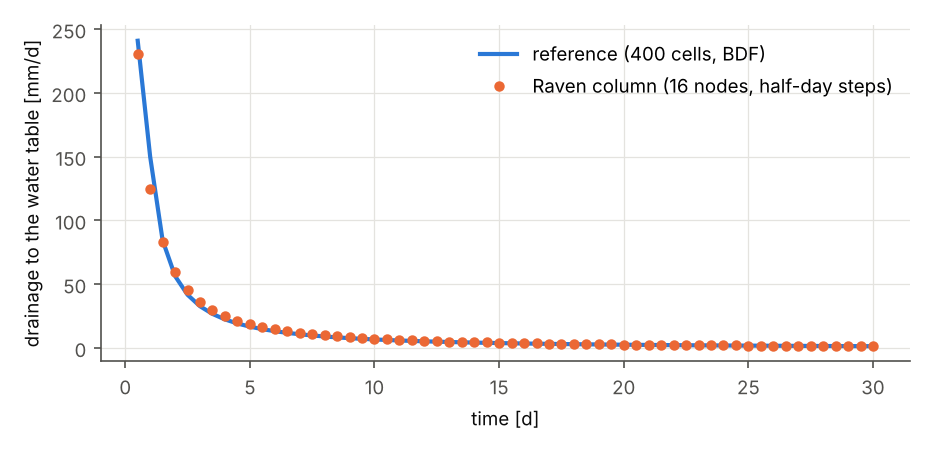
\includegraphics[width=0.49\linewidth]{figures/fig_sz_drainage.png}\hfill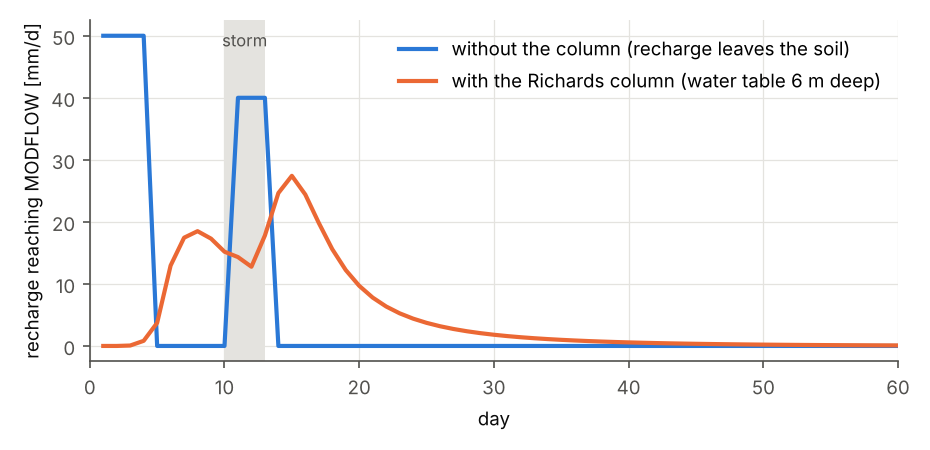
\includegraphics[width=0.49\linewidth]{figures/fig_sz_delay.png}
\caption{Left: drainage of a wet column to the water table, Raven's column against the reference solution
(step means). Right: recharge reaching MODFLOW after a 3-day storm with the water table 6~m deep
(test P1).}\label{fig:szdelay}\label{fig:szdrainage}
\end{figure}
\begin{figure}[!htbp]\centering
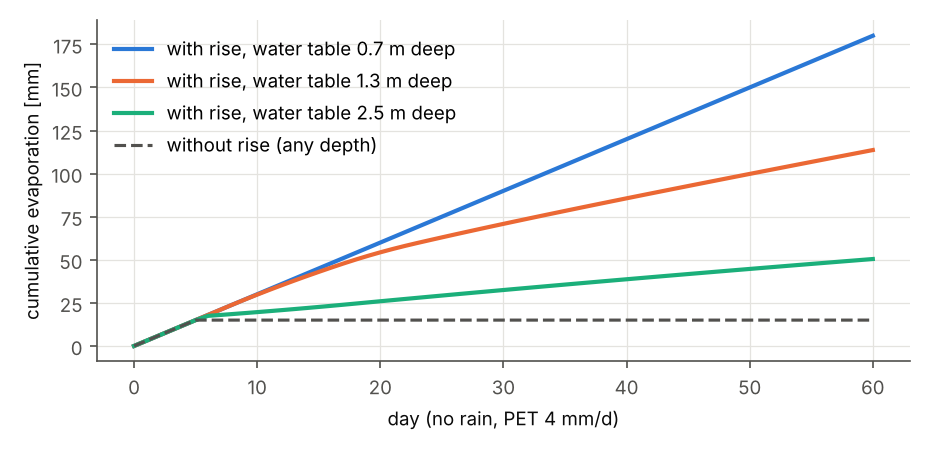
\includegraphics[width=0.49\linewidth]{figures/fig_sz_caprise.png}\hfill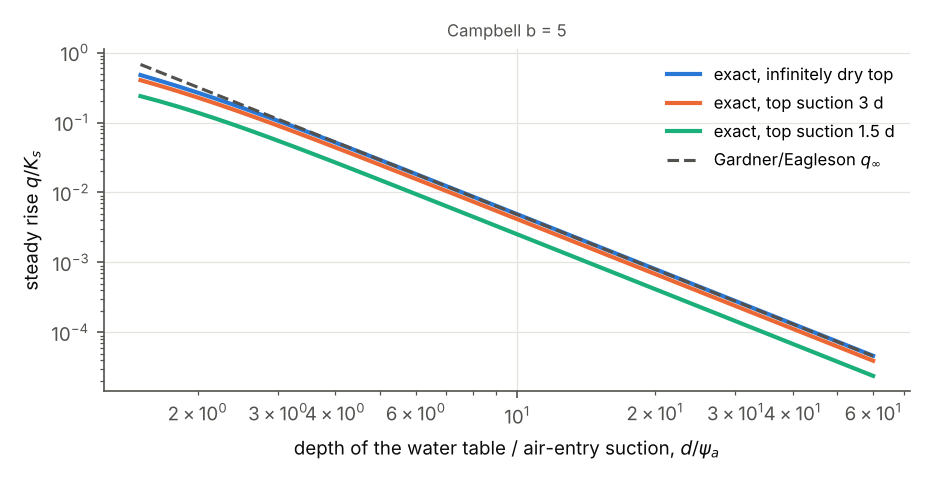
\includegraphics[width=0.49\linewidth]{figures/fig_sz_rise.png}
\caption{Left: evaporation from a drying soil over a shallow water table, with and without capillary rise (test P2).
Right: the steady rise from a water table (\ref{eq:rise}) for three suctions at the top, and Gardner's limit, which
overestimates the rise unless the soil is very dry.}\label{fig:szcaprise}\label{fig:szrise}
\end{figure}
\begin{figure}[!htbp]\centering
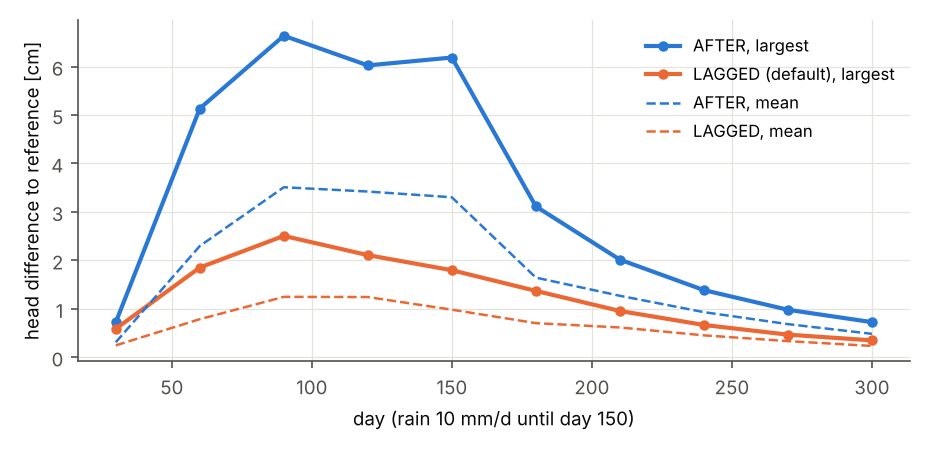
\includegraphics[width=0.56\linewidth]{figures/fig_sz_timing.png}\hfill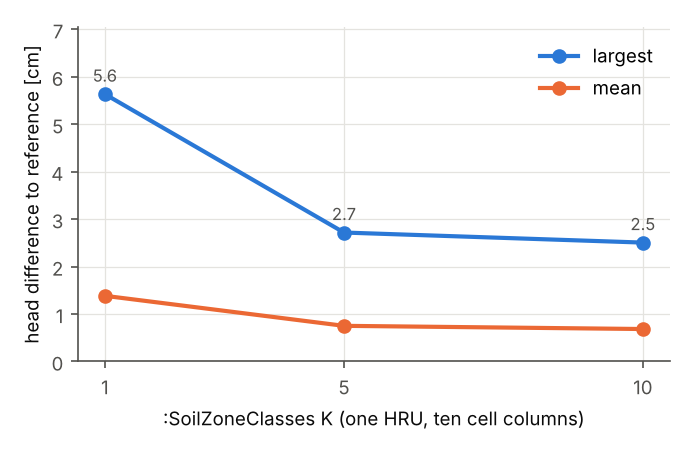
\includegraphics[width=0.42\linewidth]{figures/fig_sz_classes.png}
\caption{Left: head difference to the MODFLOW-only reference on the hillslope with the exchange after Raven's
processes (\cmd{AFTER}) and lagged (\cmd{LAGGED}, the default; test P5). Right: the same hillslope as one HRU, with Raven's
processes on 1, 5 and 10 classes of its columns (test P6).}\label{fig:sztiming}\label{fig:szclasses}
\end{figure}

\subsection{The interface iteration and MODFLOW's side}\label{sec:vszinterface}
Six scripts test the interface iteration, drained columns, heads far outside the model, negative recharge, MODFLOW's
budget as Raven books it and surface stores on soil-zone HRUs (Table~\ref{tab:vszinterface}; numbers of the quick mode, \cmd{RAVEN\_TEST\_QUICK=1}). The negative
recharge cases run in \cmd{test\_robustness.py} as R14--R22.
\begin{longtable}{P{0.13\linewidth}P{0.42\linewidth}P{0.36\linewidth}}
\caption{The interface and MODFLOW's side (\cmd{test\_interface\_stiff}, \cmd{test\_confined\_wet}, \cmd{test\_columns\_mf6},
\cmd{test\_robustness} R14--R22, \cmd{test\_mf6\_budget}, \cmd{test\_surface\_stores}).}\label{tab:vszinterface}\\
\toprule\hdr Test & Case & Result\\\midrule\endfirsthead
\caption[]{The interface and MODFLOW's side (continued).}\\
\toprule\hdr Test & Case & Result\\\midrule\endhead
S1 & low-$K_v$ top layer ($K_v$ 0.5~mm/d), wet spell from 3~m deep; columns from 1.5~m & every step converged; 4.0 (NONE) and 5.9 (RICHARDS) outer iterations per step; $F$ up to 1, column inflow 6\,530~m$^3$\\
S2 & $S_y$ 0.02, one base point per cell, rising water into a drying soil (kink drain) & converged; 4.4 / 6.0 outer iterations per step\\
S3 & explicit coupling over a 0.8~m top layer, egg-crate slope, specified head & no shortfall\\
S4 & \cmd{:SoilZoneIteration} 1 and 2 & 400 / 20 (NONE) and 400 / 60 (RICHARDS) supply-limited updates; largest take beyond the free water $2\cdot10^{-13}$~m$^3$/d\\
S5 & S4 with constant percolation and PET 5~mm/d from 1~m & take $2\cdot10^{-13}$~m$^3$/d\\
S6 & outer-iteration limit 1, iteration 0 and 1 & explicit; outputs identical\\
S7 & limits 2 and 3 & 6 of 10 steps converged (those without exchange); no ``no change \ldots to compare with''\\
S8 & connection test: stored case lowkv\_g57 without rain, $d_s$ 0.5~m, 16~m deep, head tolerance 0.05~m; default limit and limit 20 & 1 drop, its next update plain; with limit 20 the warning names the connection test at HRU 1, cell (1 1 6), fraction 0.0027 against 0\\
W1--W3 & confined layer below its bottom, generated and existing (ICELLTYPE from memory) & every step converged, no column kept wet\\
W5 & case Dc (existing, ICELLTYPE 1/0/1, ICONVERT 1, 20\,\% slope, dry then 30~mm/d) & 43 of 43 steps, 0 unconverged\\
W7 & confined model with a 10$^4$~m$^3$/d well, far heads that converge; W7c limit 3 & warned once; W7c completes, 8 MODFLOW-unconverged steps carried on, pumped head within 0.9\,\% of the default run, every warning's percentage equal to GWBudget's\\
W9, W10 & the same with limits 2 and 1 & stop: residual 2\,\% of the gross flow / the solve moved the head 1\,241~m; messages name head, cell (1 2 2), residual and causes\\
W12 & existing model with an inactive top layer, limit 2 & every interface warning names layer 2\\
W13 & the W7 model generated, \cmd{:SolverMaxOuterIterations 3} (steps 1--8 unconverged): restarts after unconverged steps & \cmd{:GWStartHeads} written after day 3 and carried unchanged through a restarted unconverged day, none after a converged day; a restart on day 4 equals the continuous run (difference 0)\\
M1--M4 & drained columns kept wet; a column delivers its inflow; \cmd{CONCEPTUAL} against a reference build; missing summary line & kept in 5 outer iterations; outflow 1.02 of the inflow; byte-identical except the balance-error \%\\
R14--R20 & negative recharge (\cmd{PERC\_GR4JEXCH}): split, cut by the top cell, hand-back, not held, existing model without \cmd{NEWTON} (confined variant), column upflow, sibling columns & identities at round-off; cut 437\,045~m$^3$; not held 3\,793 (LAGGED) / 2\,870 (AFTER)~m$^3$; not applied $-408\,000$~m$^3$, 0 with confined cells; not held only where the HRU's soil is empty (334~m$^3$)\\
R21 & a step with negative recharge in which wet unsaturated columns vanish under a water table raised by a specified head (\cmd{RICHARDS}; \cmd{KINEMATIC} in the full mode) & the vanished columns' water beyond $S_y\,\Delta h$ goes back to the soil zone as the link's rejected recharge; recharge identity 0\\
R22 & negative recharge with three depth classes, the hollow classes without a column (\cmd{RICHARDS}; \cmd{LAG} in the full mode) & MODFLOW's recharge on step 1 equals the top-cell limit (ratio 1.000000, as with one class); the cut, 2\,620~m$^3$, back to the soil zone\\
SW1--SW3 & \cmd{:SurfaceWaterExchange} on \cmd{DEPRESSION} of \cmd{:SoilZone PHYSICAL} HRUs, generated and existing model; a control with the water table above the ground at the outlet & stores' bed at the ground (model top + 1.0~m of soil zone); no discharge into the stores while every water table is below the ground; leakage 6\,135~m$^3$; existing model within $5\times10^{-6}$; control: discharge 1\,399~m$^3$\\
SW4 & restart of the control after 10 days, with a depression filled by groundwater to 64.6~mm (\cmd{DEP\_MAX} 50~mm) & the store is kept, not clipped to its maximum: Depression and the discharge into the stores equal the continuous run ($2.5\times10^{-9}$; a clip to the maximum would lose 583~m$^3$ and put the discharge 9\,\% off)\\
B1--B7 & steady existing model without STO (converged and OUTER\_MAXIMUM 3), gross flow, hourly dates, specified head under a dry cell, \cmd{:SoilZoneClasses 3}, audit guard counts & balance error $6\cdot10^{-12}$; residual equals the list file's IN$-$OUT within $1.3\cdot10^{-8}$ of the gross flow; gross flow equals TOTAL IN$+$TOTAL OUT within $5\cdot10^{-10}$; dates with times; warning names 2 columns over specified heads; no round-off as not held; guard counts 12 and 2\\
B8 & without \cmd{:SoilZone PHYSICAL}, \cmd{:SolverMaxOuterIterations} 2 (10 unconverged steps) and 1 (every step), and the Liard example (rivers and lakes) at 2: each row's residual over all its columns equals MODFLOW's negative residual on unconverged steps and 0 otherwise; run total ``discharge withheld''; at most ten warnings & step 1: 1\,039.4~m$^3$/d withheld = $-$balance error; run total 1\,062.5~m$^3$ = sum of rows; limit 1: 18\,511~m$^3$; 10 warnings (full mode)\\
B9 & \cmd{GWSoilExchange.csv} against \cmd{GWBudget.csv}: a generated model with an HRU wholly over specified-head cells, an existing model with a specified-head toe & on every date the four exchange columns summed over the HRUs equal \cmd{GWBudget.csv}'s within $2\cdot10^{-10}$ of the gross flow; the HRU over specified heads reports its base and water table\\\bottomrule
\end{longtable}
\noindent W4, W6 and W11 are reported as skipped: W4's rough-terrain cases run in \cmd{test\_rough\_terrain.py}; W6 (the
far-head warning once per ensemble member) and W11 (a head crossing the model) are not implemented as tests.

\subsection{Unsaturated-zone methods, depth classes and steady starts}\label{sec:vszmethods}
The \cmd{KINEMATIC} and \cmd{LAG} methods and the depth classes have their own tests, described with each method:
\cmd{test\_vz\_kinematic.py} K1--K9 (Section~\ref{sec:szvadosekw}), \cmd{test\_vz\_lag.py} LU, L1--L7, LS and the byte-identity
check LB (Section~\ref{sec:szvadoselag}), and \cmd{test\_vz\_classes.py} C1--C11 (Section~\ref{sec:vzclasses}). Among the
latter, C9 runs the rough-terrain case RT20 (stored existing model e43, \cmd{LAG}) with three depth classes through
\cmd{test\_rough\_terrain.py}: the saturated fraction stays within 0.0001 of the closure (limit 0.004) and no run fails; C10
writes a hotstart after a step that dropped a class column ($K=3$; after 4, 10 and 13 days): no mismatch warning, and the
restart within $7.5\times10^{-7}$ of the continuous run. \cmd{test\_vz\_initial.py} checks the steady start of
\cmd{:SoilZoneVadoseInitialFlux} (Section~\ref{sec:szvadose}):
\begin{itemize}
\item VI1, VI2, VI4: columns started at the steady profile carry their flux from the first step, with the storage at the start
in \cmd{GWModelSummary.txt}; hotstarts restore the columns; the columns' balance closes from step 1;
\item VI5: the steady start is for the flux each column receives, $(1-F)\,q$ (hummocks $\pm3$~m, water table 3~m deep,
$F=0.16$, 2~mm/d, \cmd{RICHARDS}, \cmd{KINEMATIC}, \cmd{LAG}, $K=1$ and 3): step-1 outflow = inflow = 100.8~m$^3$, 25.6~m$^3$
rejected;
\item VI6: a column that cannot carry $q$ (\cmd{K\_VERT} 1~mm/d under 2~mm/d) starts backed up: storage unchanged, outflow =
inflow = 40.000~m$^3$, 40.000 rejected, with a warning;
\item VI7: a restart with \cmd{:SoilZoneVadose NONE} from a file holding columns (\cmd{LAG}, $K=3$, negative recharge, 4 days):
a warning names the columns and their water, and \cmd{GWModelSummary.txt} reports it (248~m$^3$, the first run's final
unsaturated storage);
\item VI8: a restart with \cmd{:SoilZoneSubgrid 8} from a file written with 5 (\cmd{RICHARDS}, $K=3$): the columns' tops differ,
so they start at rest with a warning (0 against 5.37~m$^3$ written); with \cmd{:SoilZoneSubgrid 5} the written water is read exactly;
\item VI9: a restart with another method (the column case, $K=1$): written by \cmd{RICHARDS} and read by \cmd{KINEMATIC}, and
the other way round, the columns start at rest, the warning names the writing method and the run total reports the
first run's final storage (3.72 and 491~m$^3$; read as the other method's contents they would start with $+3\,669$ and
$-3\,628$~m$^3$); \cmd{RICHARDS} read by \cmd{LAG} starts with the written water;
\item VI10: a restart with a specified head added over HRU~1 (\cmd{LAG}, $K=1$, initial flux 30~mm/d): the 2 lines on its
cells are not used, and the warning and the run total give their 77.5~m$^3$ (start storage plus that volume equals the
file's water);
\item VI11: a generated model whose \cmd{:BoundaryHead} series holds the outlet cells at the start builds no column on them
(start storage 839.0~m$^3$, as with a fixed head; built there, the columns would ship 120~m$^3$ of initial-flux water to
the specified heads in step 1);
\item VI12: columns over an existing model's own specified heads (\cmd{KINEMATIC}, $K=3$, periods 3--5): a restart on day 4
rebuilds them at rest and ends them again, but only columns that held water are counted, so the two parts' run totals
add up to the continuous run's (18 columns, 225.75~m$^3$);
\item VI13: a generated model's \cmd{:BoundaryHead} series below the aquifer on days 1--3 (columns form on its cells) and
near the ground from day 4, restarted from day 3's \cmd{solution.rvc} (\cmd{LAG}, $K=1$; \cmd{KINEMATIC}, $K=3$,
\cmd{LAGGED}): the restart builds those columns from the file and ends them in its first step, so \cmd{GWBudget.csv} from
day 4 equals the continuous run's (deviation 0; day 4's recharge onto the specified heads 51.79 and 94.32~m$^3$/d).
\end{itemize}

\subsection{Input handling}\label{sec:vszinputs}
\begin{longtable}{P{0.07\linewidth}P{0.55\linewidth}P{0.30\linewidth}}
\caption{Soil zone and hotstarts: input handling (\cmd{test\_inputs.py}; short runs of the CT1 column unless stated).}\label{tab:vszinputs}\\
\toprule\hdr Test & Case & Result\\\midrule\endfirsthead
\caption[]{Soil zone and hotstarts: input handling (continued).}\\
\toprule\hdr Test & Case & Result\\\midrule\endhead
I1 & \cmd{HYDRAUL\_COND} missing for the soil class of the bottom soil-zone layer & stops (``needs HYDRAUL\_COND'')\\
I2 & \cmd{:SoilZoneIteration} with the update count only (0) & accepted; explicit, no interface update\\
I3 & \cmd{:SoilZone PHYSICAL} followed by \cmd{:SoilZone CONCEPTUAL} & the last counts: a conceptual run\\
I4 & soil-zone options under \cmd{CONCEPTUAL} & reported as ignored\\
I5 & a \cmd{:GWSoilZoneColumns} block with a column missing & reported (``do not match its soil-zone columns'')\\
I6 & the same block with its rows in another order & used (matched by cell)\\
I7 & groundwater blocks in the \cmd{.rvc} of a run without \cmd{:GroundwaterModel} & skipped; Raven's initial conditions after them apply\\
I8 & \cmd{:SurfaceWaterExchange} on a soil-zone layer & refused\\
I9 & a damaged \cmd{:GWHeads} header (\cmd{-1 2 2}; \cmd{100000 100000 100000}) & stops with a message\\
I10 & \cmd{:StartTime} in the \cmd{.rvc}, run under valgrind & no uninitialised read in \cmd{ParseInitialConditionsFile} or \cmd{TimeDifference}\\
I11 & \cmd{:BoundaryHead NOPE} beside boundary \cmd{EDGE}; \cmd{:WellFlowRate 7} with only well 1 & stop naming the series and the boundaries or wells there are; the right names run\\
I12 & \cmd{:SeepageToRaven}, \cmd{:KeepPackages}, \cmd{:MF6StartDate}, \cmd{:MF6Model} on a model Raven builds; depth classes and initial flux with \cmd{NONE}; \cmd{:SoilZoneAquiferClass} on a generated model; an unknown profile attribute; \cmd{LAYERS BOTTOM} & the four stop; the next three are reported as ignored; the last two stop\\
I13 & a missing \cmd{.rvg} file; a short \cmd{:Wells} row & named in \cmd{Raven\_errors.txt}; the message names \cmd{:Wells}\\
I14 & age tracer (no groundwater): 20 days against 7 + 7 + 6 days chained through \cmd{solution.rvc} & ages of every store and the outflow within $2\times10^{-4}$~d plus $10^{-5}$ of the age (the six digits of \cmd{Ages.csv}) of the continuous run, largest difference $10^{-4}$~d; \cmd{:StartTime} the start of each part, \cmd{:AgeTracerDatum} 2000-01-01 in the restarted parts\\
I15 & age-tracer chains across year boundaries: 1999-12-25 (7 + 7 + 6 days), 1998-12-20 (400 + 380 days; quick mode 12 + 400 + 8) & every part runs; ages within the limit of I14, largest difference $10^{-4}$~d; \cmd{:AgeTracerDatum} 1999-12-25 and 1998-12-20\\
I16 & age tracer started from the \cmd{solution.rvc} of a 30-day spin-up without it & ages 0 at the start, 1~d after the first day; no \cmd{:AgeTracerDatum}\\
I17 & EnKF, 3 members, one well, \cmd{:ExtraRVTFilename} with $-100$, $-200$, $-300$~m$^3$/d & each member pumps its own rate; a series naming no well stops the run\\
I17b & EnKF, 2 members whose \cmd{:ExtraRVTFilename} gives a \cmd{:BoundaryHead} series (99~m, then 70~m below the aquifer) to a specified head the base \cmd{.rvt} leaves fixed & each member's model is built with its series: the cells are released on days 3--6, nothing is booked onto them, and both members' \cmd{GWBudget.csv} equal the single run with the series in its \cmd{.rvt}\\
I18 & \cmd{:GWSoilZoneColumns} with \cmd{nan} or $-50$~mm, \cmd{:GWHeads} with \cmd{nan} & each stops with a message naming the block; the undamaged file runs\\
I19 & \cmd{:Transport Nitrate} (\cmd{CONCEPTUAL}, \cmd{PHYSICAL}) and \cmd{:Transport AGE} with \cmd{:GroundwaterModel MODFLOW6}; the same model without groundwater & the coupled runs stop naming the constituent; the run without groundwater completes\\
I20 & a specified head with \cmd{HEAD} 0 (below every cell) and a \cmd{:BoundaryHead} series of 99.5~m; the same without the series & placed by the series: 2 cells, flow 1\,390~m$^3$; without it no cell and a warning naming the boundary, its head and the highest cell bottom\\
I21 & head boundary \cmd{EDGE} (\cmd{HEAD} 90) with a series of 99~m on day 1, then 90~m; layer 1 from 100 to 97~m: (a) a GHB (\cmd{LAYERS TOP}) against an aquifer at 95~m; (b) a CHD (\cmd{LAYERS TOP}); (c) a CHD (\cmd{LAYERS ALL}, 99~m for 3 days), restarted on day 4 & (a) the GHB drains on days 2--6 ($-7\,915$ to $-2\,275$~m$^3$/d), as with \cmd{HEAD} 90 alone; a series of 90~m gives the outputs of \cmd{HEAD} 90; (b) the water table falls below 97~m (93.8 to 92.9~m): no cell is held at the bottom of layer 1; (c) the restarted run has the same 4 CHD cells and the same flows and heads as the continuous run\\
I21 (d) & a column with no cell held: 8 HRUs, the last wholly on \cmd{EDGE} (\cmd{LAYERS ALL}), rain 20~mm/d, a series of 99~m on days 1--2 and 70~m (below the aquifer) on days 3--6; \cmd{CONCEPTUAL} and \cmd{PHYSICAL} & days 3--6: CHD flow 0 and nothing booked onto specified-head cells; MODFLOW's recharge equals Raven's (\cmd{CONCEPTUAL}); the column's soil-zone link exchanges 425 to 42~m$^3$/d with the aquifer (\cmd{PHYSICAL}); every identity holds\\
I21 (e) & \cmd{LAYERS TOP}, \cmd{HEAD} 90 and a series of 99~m on every day, CHD and GHB & the cells of layer 1 only (2), none switched off\\
I21 (f) & a steady-state first period at 90~m (series 90, 99, 99, 90, 90, 99~m) & the run total counts the steady period's 2 cells: 8 cell-steps against 6 without it\\
I22 & \cmd{:InitialGWHeads ELEVATION 98,5}, \cmd{H98.5}, \cmd{0x62}, \cmd{98.5}, \cmd{98.5\# note} and \cmd{98.5 \# note}; \cmd{:InitialGWHeads FROM\_PROFILE 0}; a \cmd{:GWHeads} value \cmd{98.1x} & the first three stop naming the command and the token (surplus value '5'; not a number), the next three start at 98.5~m; \cmd{FROM\_PROFILE 0} stops (takes no value); the damaged value stops naming the block\\
I23 & two \cmd{:SpecifiedHeadBoundary} commands on the same file (\cmd{HEAD} 99 and 99.5); two \cmd{:GeneralHeadBoundary} commands on it & the first stops before MODFLOW starts, naming both boundaries and the cell; the second runs\\\bottomrule
\end{longtable}

\subsection{Robustness}\label{sec:vszrobust}
\begin{longtable}{P{0.07\linewidth}P{0.55\linewidth}P{0.30\linewidth}}
\caption{Soil zone: robustness (\cmd{test\_robustness.py}; hard cases of the interface). R14--R22, the negative-recharge
cases, are in Table~\ref{tab:vszinterface}.}\label{tab:vszrobust}\\
\toprule\hdr Test & Case & Result\\\midrule\endfirsthead
\caption[]{Soil zone: robustness (continued).}\\
\toprule\hdr Test & Case & Result\\\midrule\endhead
R1 & stiff flat column: drainable porosity 0.02 against $S_y=0.25$, high conductance & every step converged; at most 12 updates, 27 outer iterations\\
R2, R2c & one HRU over ten cells against ten one-cell HRUs; R2c with constant-rate percolation & outflow $-0.2\,\%$, MODFLOW recharge ratio 1.00; R2c outflow $-0.2\,\%$\\
R3 & \cmd{RECHARGE\_DELAY} with \cmd{:SoilZone PHYSICAL} & refused\\
R4 & a smoothing depth below 0.1~m & warned\\
R5 & hourly steps, smoothing depth 0.001~m & no unconverged step; MODFLOW error $1.1\times10^{-11}$\\
R6 & slope 0.1 with $5\times5$ DEM points per cell & converged; at most 8 updates\\
R7 & explicit mode (\cmd{:SoilZoneIteration 0}) & no shortfall\\
R8 & one column $10^{-6}$~mm wetter than the others & heads stay uniform ($3.7\times10^{-9}$~m)\\
R9 & hotstart columns that cannot hold the \cmd{.rvc} layer split & 4\,000~m$^3$ redistribution reported in step 1, 0 later\\
R10 & water rising into a thin soil on a steep, low-storage slope, update budget 1 and explicit mode & no shortfall\\
R11 & explicit mode on the R2 hillslope against the iterated run & outflow within 0.6\,\%\\
R12 & explicit mode, 15 outer iterations, water rising into cells dry at the head of linearization & converged; outflow within 0.6\,\%; MODFLOW error $10^{-7}$\\
R13 & stiff low-storage slope, budget 1, 12 outer iterations, MODFLOW unconverged & neither residual nor shortfall handed to Raven: outflow 1.01 times the iterated run's\\
R15b & a negative-recharge cut on a draining soil zone: 8.67~mm cut while the wet soil drains & soil zone after step 1 at least its field-capacity water (126.08 against 120~mm)\\\bottomrule
\end{longtable}

% Verification on rough terrain (tests/soilzone/test_rough_terrain.py, rough_models.py, rough_ext.py, rough_cases/).
\section{Rough terrain}\label{sec:vrough}
The tests of Section~\ref{sec:vsoilzone} use planar hillslopes. Real ground is irregular: slopes change within a cell,
the land holds pits, closed depressions, cliffs and ridges, the DEM is finer or coarser than the grid and may end inside
it, and the MODFLOW layers slope, thin out and pinch against bedrock. The rough-terrain suite
(\cmd{tests/soilzone/test\_rough\_terrain.py}) draws such cases at random from a seed, runs each with every
unsaturated-zone method and checks every run against rules that hold whatever the ground looks like. A seed always gives
the same case, so every failure can be replayed (\cmd{--case}).

\subsection{What the cases vary}
Every fourth seed couples an existing MODFLOW~6 model written by the suite (\cmd{rough\_ext.py},
Section~\ref{sec:vexisting}); the others let Raven build the model (\cmd{rough\_models.py},
Section~\ref{ch:layers}). Table~\ref{tab:vroughvary} lists the ranges.
\begin{table}[!htbp]\centering
\caption{What the rough-terrain cases vary (\cmd{rough\_models.gen\_spec}; existing models: \cmd{rough\_ext.ext\_spec}).}\label{tab:vroughvary}\small
\begin{tabular}{P{0.2\linewidth}P{0.74\linewidth}}\toprule\hdr
Item & Range\\\midrule
ground & a plane sloping 0--30\,\% in any direction plus roughness: spectral noise, bumps, pits, closed depressions, cliffs (steps a few metres wide, or sharper than the DEM) and ridges; relief within a cell from 0.05 to 6 times the soil-zone thickness $D$\\
DEM & resolution 0.08--1.6 cells; NODATA holes; a DEM that ends inside the grid (cells partly without land samples)\\
grid and HRUs & cells of 25--150~m, 4--9 by 3--6 cells; a tiling of HRUs cut at random positions (on and off cell edges, one-cell HRUs); domain edges on or inside cells; \cmd{:MinCellCoverage} 0.1--0.5\\
soil & two soil profiles by position, two layers, $D$ 0.3--3~m; Campbell retention for the capillary rise; \cmd{PERC\_CONSTANT} or \cmd{PERC\_GAWSER\_CONSTRAIN}\\
aquifer (generated) & two aquifer profiles by position, 1--3 layers of 2--3 classes ($K_h$ 0.05--30~m/d, $K_v$ down to $10^{-2.5}K_h$, $S_y$ 0.02--0.3, retention for the columns); thin layers (0.2--0.8~m); sloping bedrock raster (or \cmd{DEFAULT\_BEDROCK\_DEPTH}), so layers slope, pinch out, are clipped at bedrock and become pass-through cells; bedrock at least $\max D+1.0123$~m below the land, except in outcrop cases (bedrock above the soil-zone base under a whole HRU)\\
aquifer (existing) & DIS or DISV (irregular quadrilaterals); top = mean land $-D$, moved up or down by up to $D$; 1--3 layers whose thicknesses tilt across the model, pass-through cells (\cmd{IDOMAIN}~$-1$) where a layer thins below 0.5~m, inactive columns and columns with an inactive first layer (\cmd{IDOMAIN}~0); a confined bottom layer in some models; \cmd{NEWTON} in most models, a few without it\\
water & \cmd{:SoilZoneSubgrid} 1, 3, 5, 9; \cmd{SEEPAGE\_SMOOTHING\_DEPTH} 0.02--0.5~m; 40--90 daily steps; mean rain 8--45~mm/d on 10--40 wet days (daily 2.4--77~mm/d) between dry spells; soil evaporation 0--4~mm/d; start deep (3--15~m), shallow (0.2--2~m) or at the land; a specified head along the low edge; \cmd{:SoilZoneCapillaryRise} on, off or default; \cmd{:SoilZoneExchangeTiming} \cmd{LAGGED} or \cmd{AFTER}\\
\bottomrule
\end{tabular}
\end{table}

\subsection{What every run is checked for}
\begin{description}
\item[Run] The run completes, or stops with a justified message (below).
\item[Finite] No NaN or Inf in any output table, no non-finite head, no \cmd{HDRY} head in an active cell under \cmd{NEWTON}.
\item[Balances] The identities of Section~\ref{sec:audit} close within the standard limits (recharge $5\times10^{-9}$,
soil zone and unsaturated zone $10^{-8}$, MODFLOW $10^{-5}$ of the recharge, Raven $10^{-5}$~mm), and no soil-zone
shortfall is booked on a step whose interface converged.
\item[Layers] For generated models, \cmd{TOP}, \cmd{BOTM} and \cmd{IDOMAIN} as MODFLOW read them equal an independent
construction from the DEM, the bedrock raster and the profiles (Section~\ref{ch:layers}) within $10^{-6}$~m.
\item[Bases] The soil-zone base of every HRU equals the overlap-weighted land surface of its cells less $D$ (existing
models: the top of the top active cell).
\item[Saturated fraction] With \cmd{:SoilZoneVadose NONE}, the saturated fraction of every HRU equals an independent
closure --- the cell's DEM samples less $D$, none below 1~mm above the top cell's bottom, smoothed over $d_s$ --- at a head
between the top cells' heads at the start and the end of the step, on every converged step, within 0.02. With a column
method the difference is reported only: the fraction reported for a link whose column carries the step is the
connection's, not the one that rejected the recharge.
\item[Physics] $0\le F\le1$; soil water within $[0,$ capacity$]$; rejected recharge and overflow $\ge0$; with
\cmd{NONE} the rejected recharge is at most the HRU's recharge, positive only where $F>0$, and $F$ times the recharge on
HRUs over one cell; with a column method the rejected recharge of a step is at most its recharge plus the columns'
storage at its start.
\item[Heads] With a column method, no water table more than 5~m above the highest land sample of its cell, unless the
\cmd{NONE} run of the same case lifts it to within 1~m of that height.
\item[Convergence] Steps on which MODFLOW or the interface did not converge are counted; more than 5\,\% fails the case.
\end{description}
A run whose failures are all known ones is reported as a known failure (XFAIL): the suite keeps one known pattern, an
interface left unconverged where the land lies below the top cell's bottom, and no open case. A shortfall is never a known
failure, and a regression case's own checks are added before this is decided: any other failure makes the run fail.

\paragraph{Justified stops.} A run may stop without failing in three situations: an outcrop case (\emph{HRU \dots\ does
not overlap any active groundwater cell}); an existing model without \cmd{NEWTON} (\emph{:SoilZone PHYSICAL needs an
existing model that uses the Newton-Raphson formulation}); and a diverged solve (\emph{heads are not finite}, or a head
far outside the model on an unconverged step) that MODFLOW~6 repeats on its own. For the last, the suite runs the case's
MODFLOW model through the library without Raven's packages, with a drain at the top of every column as the only outlet
and no recharge, for the run's duration; the stop is justified only if those heads become non-finite or move by more
than $10^6$~m within the outer iterations. A column held 1~mm above its bottom (Section~\ref{sec:drained}) is reported,
not a failure.

\paragraph{Regression cases.} Twenty cases run first (RT1--RT20, Table~\ref{tab:vroughprob}): RT1 is a flat hillslope (the
configuration of P3 without columns) on which the rejection must follow the converged head: with the saturated fraction of
an earlier iterate it would reject 15\,\% of the recharge where the closure at the step's heads allows at most 5\,\%;
RT2--RT20 are stored cases (\cmd{rough\_cases/*.json}, each with its spec and the meta data the checks use) of the hardest
situations the suite draws. Each has
its own checks besides the above: RT6, RT11--RT13 and RT19 must complete (no stop at all), and RT20 (stored existing model e43,
\cmd{LAG}) must hold the saturated fraction to the closure within 0.004 with any method: its land lies in
places within the 1~mm band above the top cell's bottom, where no sub-grid base may lie. \cmd{--case} applies these checks
too when it replays a stored case.

\subsection{Results}
Table~\ref{tab:vroughres} summarizes the suite's 400 default seeds run with each of the four methods
(\cmd{--methods NONE,RICHARDS,KINEMATIC,LAG}, 1\,620 runs with the regression cases; the script's default runs
\cmd{NONE} and \cmd{RICHARDS} only). No run failed and none was a known failure. Every run that completed (1\,567 of
1\,620) closed all balances within the limits above (largest values: recharge identity $4.5\times10^{-10}$, soil-zone
identity $9.9\times10^{-10}$, unsaturated-zone identity $4.6\times10^{-10}$, MODFLOW $7.7\times10^{-6}$ of the recharge,
Raven $10^{-11}$~mm; largest shortfall $4\times10^{-14}$). The independent geometry agreed everywhere: layers to
$5\times10^{-8}$~m, bases to $5\times10^{-8}$~m. On converged steps the saturated fraction agreed with the closure to
0.0022 with \cmd{NONE} (limit 0.02); with a column method it is reported (largest difference 0.0027 with \cmd{RICHARDS}
and \cmd{LAG}, 0.0020 with \cmd{KINEMATIC}).
\begin{table}[!htbp]\centering
\caption{Rough-terrain suite, default seeds and regression cases, one depth class.
Run times depend on the machine and its load (two cores shared with another test suite).}\label{tab:vroughres}\small
\begin{tabular}{P{0.36\linewidth}P{0.13\linewidth}P{0.13\linewidth}P{0.13\linewidth}P{0.13\linewidth}}\toprule\hdr
 & \cmd{NONE} & \cmd{RICHARDS} & \cmd{KINEMATIC} & \cmd{LAG}\\\midrule
runs & 407 & 408 & 401 & 404\\
completed / justified stops & 393 / 14 & 395 / 13 & 388 / 13 & 391 / 13\\
known failures / failures & 0 / 0 & 0 / 0 & 0 / 0 & 0 / 0\\
time steps of completed runs & 25\,753 & 25\,809 & 25\,350 & 25\,528\\
steps with the interface unconverged & 0 & 0 & 0 & 0\\
steps with MODFLOW unconverged & 0 & 0 & 0 & 0\\
runs with the water table $>5$~m above the land; largest & 44; 94.2~m & 43; 94.2~m & 40; 94.2~m & 42; 94.2~m\\
MODFLOW outer iterations per step (mean) & 6.34 & 5.83 & 5.70 & 7.20\\
mean run time [s] & 0.16 & 0.22 & 0.18 & 0.19\\\bottomrule
\end{tabular}
\end{table}
The justified stops are the outcrop cases (g14, g33, g58, g61, g162, g223, g266), the existing models without
\cmd{NEWTON} (e36, e96, e200, e256, e316, e356: 6 of the 100 existing models, the others use it; with \cmd{NONE} also
the regression case RT17, which tests this stop), and stops that MODFLOW alone repeats (none). The run counts differ
between the methods because the regression cases run with one method each. Water tables far above the land occur where
the land is steep and the top layer's vertical conductivity low: the largest, 94.2~m, is seed g274 (slope 16\,\%,
150~m cells, $K_v=0.0047$~m/d) with every method, \cmd{NONE} included, so it comes from the aquifer model, not from the
columns (\cmd{--case 274}). No column method lifts such a water table over \cmd{NONE}'s (largest difference 0.0~m at
the 0.1~m resolution of the report); the column methods have fewer such runs than \cmd{NONE}. With
\cmd{:SoilZoneVadoseClasses 3} (\cmd{--vzclasses 3}, the same 1\,620 runs) the suite gives 0 failures and 0 known
failures, with the same completed runs and justified stops, no unconverged step, the same balance limits (largest
MODFLOW identity $8.3\times10^{-6}$), 0.0031 as the largest reported difference of the saturated fraction (\cmd{LAG}),
44, 43, 41 and 43 runs (\cmd{NONE}, \cmd{RICHARDS}, \cmd{KINEMATIC}, \cmd{LAG}) with the water table more than 5~m above the land (largest 94.2~m, g274, as
with one class; the column methods lift it by at most 0.1~m over \cmd{NONE}'s), 5.72, 5.61 and 7.13 outer iterations per
step (\cmd{RICHARDS}, \cmd{KINEMATIC}, \cmd{LAG}) and mean run times of 0.34, 0.22 and 0.23~s. RT20 holds the closure to
0.0001 with three classes (0.0002 with one class; limit 0.004). The water table of RT20's \cmd{LAG} run with three
classes differs from that with one class by at most 0.35~m: it is lower by up to 0.16~m during the first two weeks of the
rain (the upper classes' longer columns hold more of the rain on its way down), and higher by up to 0.35~m late in the
dry spell that follows the rain (day 67, as they release it).

\begin{table}[!htbp]\centering
\caption{The regression cases of the rough-terrain suite: the situation each one stores and the part of the coupling that
handles it. They run first in the suite.}\label{tab:vroughprob}\small
\begin{tabular}{P{0.44\linewidth}P{0.32\linewidth}P{0.15\linewidth}}\toprule\hdr
Situation & Handled by & Case\\\midrule
rejection on a converged step & the rejection follows the converged head & RT1\\
columns over cells filled to the soil-zone base & the columns' hand-back and the heads check & RT14--RT16\\
drained columns, which would leave MODFLOW's solve singular & a drained column is held 1~mm above its bottom once per step (and once more on any later solve in that step) & RT6, RT11--RT13\\
an existing model without \cmd{NEWTON} whose top cells dry & a start-up stop: \cmd{NEWTON} is required & RT17\\
\cmd{LAG} on a slowly permeable slope (g350), which must complete & the \cmd{LAG} cascade (Section~\ref{sec:szvadoselag}) & RT19\\
sub-grid bases in the 1~mm band below the lowest drain level & bases clipped at the top cell's bottom + 1~mm & RT3, RT20\\
the saturated fraction with three depth classes (a connection head away from MODFLOW's head) & the connection test (Section~\ref{sec:szinterface}) & RT20, also with three depth classes (C9)\\
slowly permeable or low-yield top cells, dried top cells, DISV models & head-dependent rejection, upward flow from a lower cell & RT2, RT4, RT5, RT7--RT10, RT18\\
\bottomrule
\end{tabular}
\end{table}

\begin{figure}[!htbp]\centering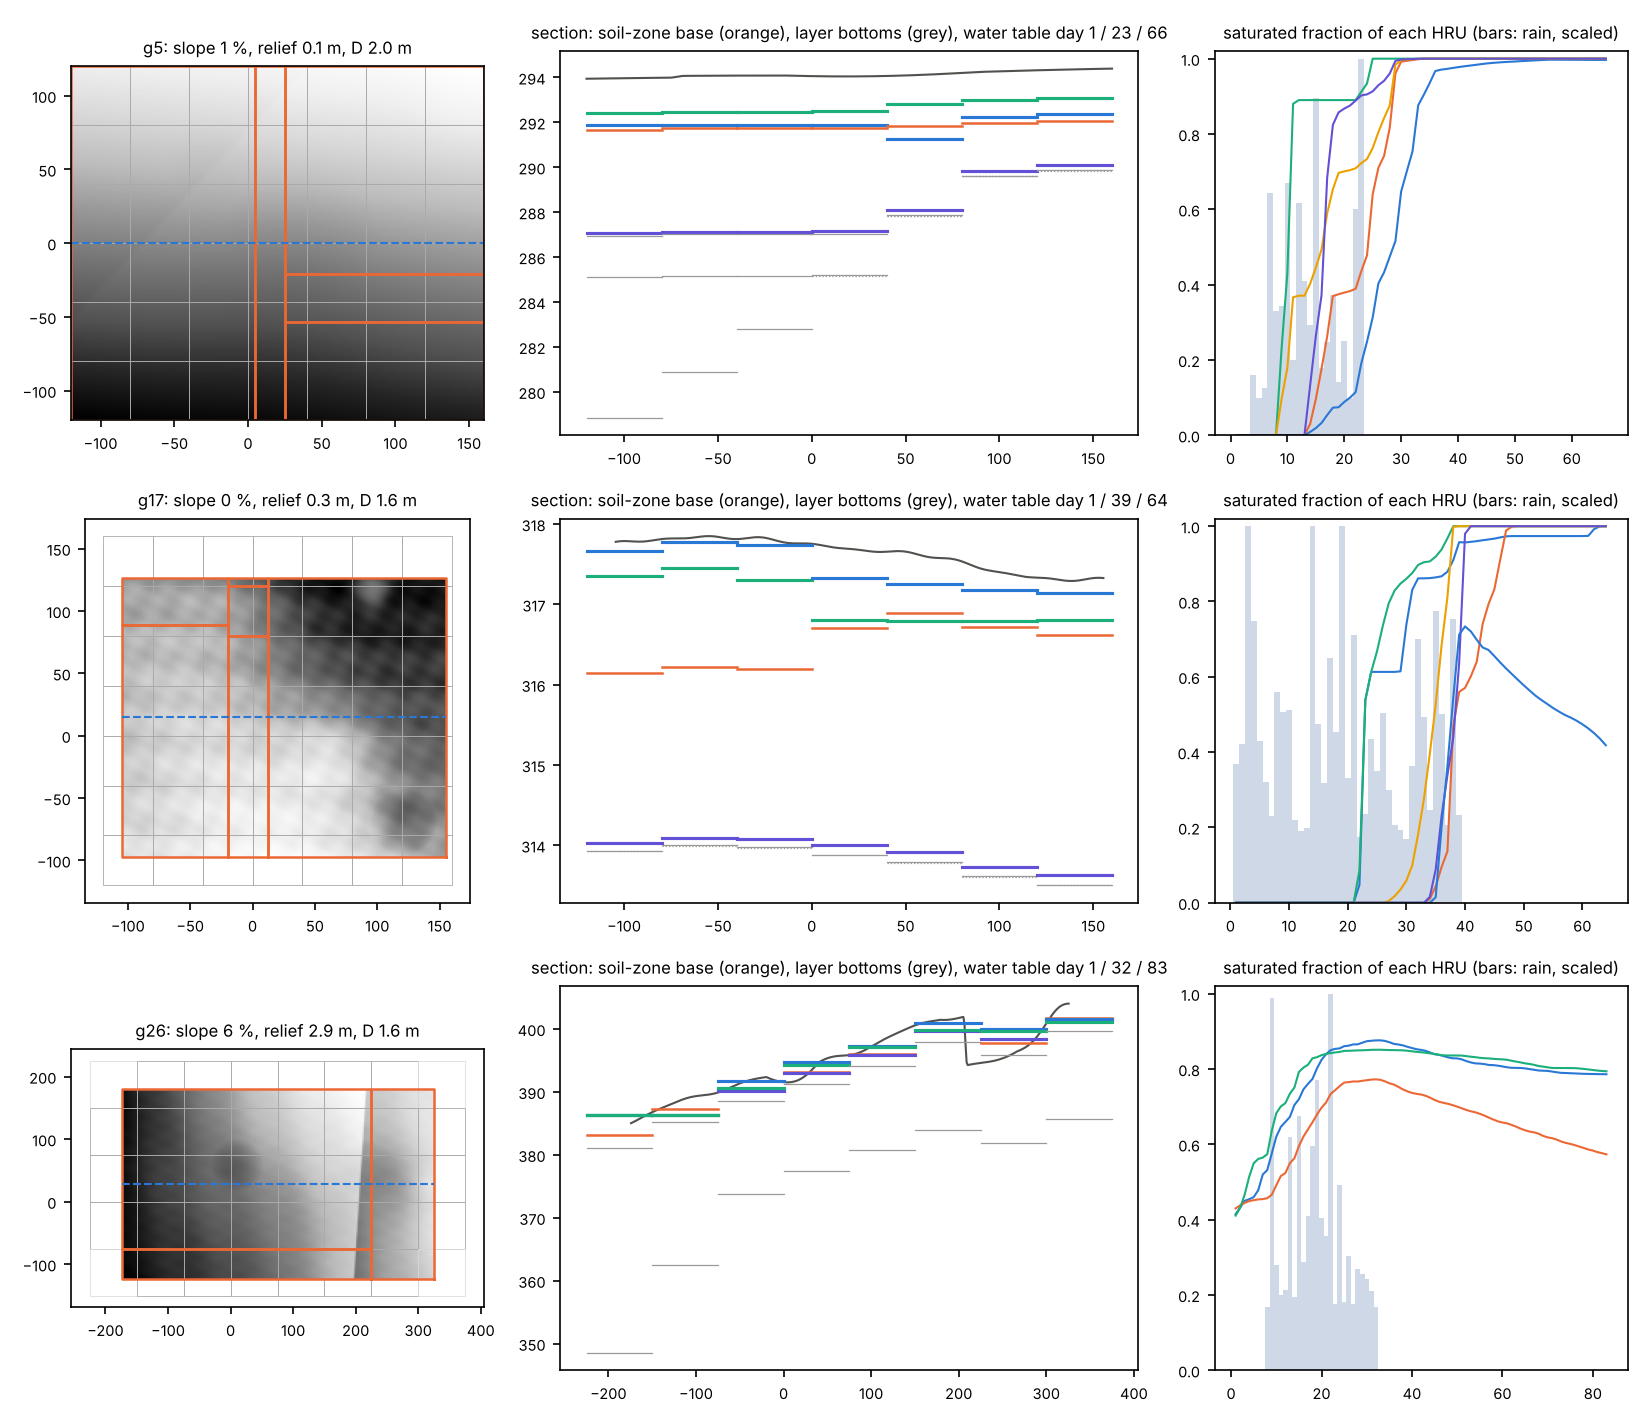
\includegraphics[width=\linewidth]{figures/fig_rough_cases.png}
\caption{Three cases of the suite (\cmd{:SoilZoneVadose NONE}). Left: DEM (shaded), grid cells and HRUs (orange); the
dashed line marks the section. Middle: land along the section, soil-zone base, MODFLOW layer bottoms of the cells it
crosses and the water table at the start, at the end of the rain and at the end of the run. Right: saturated fraction of
each HRU over the run.}\label{fig:vrough}
\end{figure}

\begin{refcard}{rough-terrain suite}
\begin{tabular}{@{}P{0.42\linewidth}P{0.53\linewidth}@{}}
\cmd{python3 test\_rough\_terrain.py} & regression cases RT1--RT20 and 400 seeds, \cmd{NONE} and \cmd{RICHARDS}\\
\cmd{--quick} / \cmd{--full} & 40 / 1\,500 seeds (\cmd{RAVEN\_TEST\_QUICK=1}: quick)\\
\cmd{--methods NONE,RICHARDS,KINEMATIC,LAG} & the methods run for every seed (and the regression cases whose method is listed)\\
\cmd{--vzclasses K} & \cmd{:SoilZoneVadoseClasses K} for every run\\
\cmd{--seeds a-b}, \cmd{--family gen|ext|both} & part of the seeds; generated or existing models only\\
\cmd{--case 57:RICHARDS}, \cmd{--case x43:LAG} & replay seed 57 (\cmd{x}: as an existing model); a column method is preceded by the case's \cmd{NONE} run\\
\cmd{--case rough\_cases/band\_e43.json:LAG} & replay a stored case with its own checks (or a run folder's \cmd{case.json}); the exit status is the run's\\
\cmd{--keep}, \cmd{--noreg} & keep the run folders; skip the regression cases\\
\end{tabular}
\end{refcard}


\section{Build checks}\label{sec:vbuild}
\cmd{tests/cmake\_checks.py} runs 22 offline configure checks of Raven's CMake integration of MODFLOW~6
(Section~\ref{sec:building}) in about a minute, without compiling Raven (Table~\ref{tab:vcmake}). \cmd{-{}-selftest} puts
the defect each check guards against back into a copy of the source and shows that the check then fails.
\cmd{tests/mf6version\_check.py} checks Raven's run-time version guard with a stand-in library, and
\cmd{tests/mf6lib\_check.py} how \cmd{tools/get\_mf6.py} chooses the release for each platform and where Raven finds the
library. The installed folder is checked by \cmd{cmake/RavenMF6InstallCheck.py}: it runs the installed Raven on a tiny coupled
model and checks that it used the library beside it and that every Fortran runtime library it loaded lies in that folder.

\begin{longtable}{P{0.07\linewidth}P{0.86\linewidth}}
\caption{CMake checks (\cmd{tests/cmake\_checks.py}).}\label{tab:vcmake}\\
\toprule\hdr Check & What is checked\\\midrule\endfirsthead
\caption[]{CMake checks (continued).}\\
\toprule\hdr Check & What is checked\\\midrule\endhead
1 & the default on Linux aarch64 without the source tools falls back to \cmd{OFF} with a warning naming \cmd{-DRAVEN\_MF6=OFF}; the configure succeeds\\
2 & that default survives a reconfigure and becomes \cmd{SOURCE} when the tools appear and the repository answers\\
3 & run path: the library from the build tree and from a moved install (\cmd{\$ORIGIN})\\
4 & \cmd{PATH} mode installs a symbolic link or a renamed library as \cmd{libmf6.so}\\
5 & \cmd{libmf6\_version.txt} and the package name (unknown for \cmd{PATH}, the \cmd{meson.build} version for zips and sources)\\
6 & offline options name their mode; options of another mode are reported as ignored; an unpinned zip is warned about\\
7 & meson gets the Fortran compiler of \cmd{FC}\\
8 & a meson whose version cannot be read is named as such\\
9 & a staged install (\cmd{DESTDIR}) gets \cmd{libgfortran.so.5}\\
10 & without git the default falls back, \cmd{SOURCE} stops naming git, and \cmd{RAVEN\_MF6\_SOURCE\_URL} needs none\\
11 & a replaced zip is unpacked again, an unchanged one is not\\
12 & Windows AMD64 and ARM64 (emulated)\\
13 & the package version from a \cmd{v6.7.2.tar.gz} source URL; an unpinned zip is ``not checked''\\
14 & a wrong \cmd{RAVEN\_MF6\_ZIP\_SHA256} stops the configure (local and downloaded zips)\\
15 & offline default: with the source tools but an unreachable git repository the default falls back at configure time to \cmd{PREBUILT} (a local release folder: the library target builds without network) or, with no release either, to \cmd{OFF} with a warning; a reachable repository gives \cmd{SOURCE}\\
16 & a single-configuration generator without \cmd{CMAKE\_BUILD\_TYPE} configures \cmd{Release} (\cmd{-O3 -DNDEBUG}); a given \cmd{Debug} is kept\\
17 & a MODFLOW version below 6.5.0 as \cmd{RAVEN\_MF6\_VERSION} (\cmd{SOURCE} and \cmd{PREBUILT}), in a zip's or a source folder's \cmd{meson.build} or in an archive name stops the configure naming 6.5.0; 6.7.0 configures with a warning naming 6.8.1\\
18 & runtime bundling, emulated on Linux: macOS with Mach-O stand-ins (\cmd{@rpath} chains resolved through \cmd{LC\_RPATH}, every reference rewritten to \cmd{@loader\_path}, every edited file signed); Windows with stand-in \cmd{objdump} and \cmd{dumpbin} (the DLLs \cmd{libgfortran-5.dll} imports installed)\\
19 & messages for a folder given as \cmd{RAVEN\_MF6\_PATH} and for a SHA-256 that is not 64 hex digits\\
20 & \cmd{PATH} mode on Linux: a gfortran-built library without a run path gets \cmd{\$ORIGIN} from \cmd{patchelf} and loads the runtime installed beside it; without \cmd{patchelf} a warning says that it loads the system's runtime; a library that has \cmd{\$ORIGIN} is left as it is\\
21 & \cmd{RAVEN\_MF6=OFF} (given, and as the default's fallback): the configure says that \cmd{cmake --install} installs Raven alone, and the install does so with a message\\
22 & the default's offline fallback to \cmd{OFF} with the source tools installed names the network; without meson the warning asks for the source tools\\\bottomrule
\end{longtable}
\noindent Real macOS and Windows systems are not part of these checks: the bundling there is emulated.

\section{Code checks}\label{sec:codeaudit}\label{sec:sanitizer}
\begin{itemize}
\item \textbf{Review:} line-by-line reading of the coupling's files and of every changed Raven file --- units, signs,
indices, order of operations, and that each volume is applied once on each side.
\item \textbf{Compilers and static analysis:} GCC and Clang, unoptimised and optimised: no warnings with \cmd{-Wall -Wextra
-Wshadow} in the coupling's files (with and without NetCDF); none from cppcheck and clang-tidy. A Windows build (MinGW) run
under Wine gives the Linux results to rounding.
\item \textbf{Sanitizers:} complete builds with AddressSanitizer and UndefinedBehaviorSanitizer, run on random set-ups covering
every option, an ensemble and a restart, on one random set-up of every grid type, on the faulty-input set-ups of
Section~\ref{sec:mf6files}, on seven reservoir and ensemble cases and on three years of the Liard model: no memory error and
no undefined behaviour. The only reported leaks are allocated inside the MODFLOW library.
\item \textbf{valgrind:} a hotstart with \cmd{:StartTime} (test I10, Table~\ref{tab:vszinputs}) reads no uninitialised value
in the hotstart code. valgrind reports uninitialised reads in two routines of Raven itself that the coupling does not touch
(Section~\ref{ch:limits}, known issues).
\end{itemize}

\section{Option combinations}\label{sec:vcombinations}
\cmd{tests/combinations.py} runs small synthetic models (four HRUs on a slope, 100~m cells) across a matrix of options and
checks every water identity on each run. The exchanges (water-table ET, a river, surface stores, a reservoir, a well, a
general-head and a specified-head boundary, each placed at the height of the ground where it lies) are combined all
together and one at a time; each under plain conditions, dry top cells (a 1~m top layer above the water table) and
negative recharge (\cmd{PERC\_GR4JEXCH}); with \cmd{CONCEPTUAL} and \cmd{:SoilZone PHYSICAL} (with
\cmd{:SurfaceWaterExchange} on the surface stores). The lake loses water where it lies on the ground (its stage above the
ground of its cells) and gains it as a pit lake half over the specified-head cells (its stage below the specified head);
water-table ET draws on a PET the soil cannot meet from a water table within the extinction depth. The unsaturated
columns (\cmd{RICHARDS}, \cmd{KINEMATIC}, \cmd{LAG}, one and three depth classes) run under negative recharge, a water table
rising through them (the columns vanish) and dry top cells. A boundary group switches cells off and on with
\cmd{:BoundaryHead} series (also every cell of a column, which is then an ordinary column) and switches an existing
model's own specified heads on under a lake. Every case except the \cmd{:BoundaryHead} series cases of the boundary group (6 in quick mode, 8 in full mode; generated model only) runs with the model Raven builds and as an existing model (with
\cmd{NEWTON}, without it for \cmd{CONCEPTUAL}, and converted to feet and seconds, the model's own river, well and boundaries
included). On every run: MODFLOW's balance, the recharge, soil-zone and unsaturated-column identities, Raven's balance, the
river, surface-store and reservoir books, the seepage returned, the run totals against their columns, and no HDRY or NaN in
the groundwater outputs. Every run must also move water through each exchange and stress its case names, and lists the
volumes moved: a case whose exchange moves none fails (in an existing model without \cmd{NEWTON} with dry top cells, which
MODFLOW takes out of its solve, the surface stores, the lake and the river must move none). The quick mode runs 311 runs
of 8 days (a few minutes), the full mode 393 runs of 15 days, with half-day steps too.
\cmd{tests/reservoir\_checks.py} checks the reservoir exchange where a lake's cells cannot all take seepage (existing and
generated models), its bed under \cmd{:SoilZone PHYSICAL}, and the run total of gains MODFLOW does not supply. One result is reported
apart as known: where a reservoir's stage falls back below its weir crest while groundwater feeds it, Raven's balance error
equals the reservoir routing's own balance error (a few m$^3$, \cmd{ReservoirMassBalance.csv}); the coupling's books hold.
The error comes from Raven's reservoir routine, which stops its stage iteration at a change of 0.1~mm next to the kink of the
weir's outflow curve; base Raven gives the same without groundwater (Section~\ref{ch:limits}). It is excused only on steps
whose stage lies within 5~mm of the crest and only up to $2.5\times10^{-4}$~m times the lake's area per step (10~m$^3$ for
the test lake); any other balance error fails. A self-test checks the rule on a run's outputs: an unbooked 5\,000~m$^3$
added to the lake's routing error fails, as does 2~m$^3$ on a step 0.3~m below the crest; 2~m$^3$ at the crest is known.

\section{Running the tests}\label{sec:runtests}
\cmd{python3 tests/run\_all.py} runs every test of this chapter (the unit tests, the file and input checks, the Thiem,
restart, lake and grid tests, the budget cross-check, both randomized harnesses, the existing-model tests, the soil-zone tests
of Section~\ref{sec:vsoilzone} and the rough-terrain suite: in full mode 400 seeds with all four unsaturated-zone methods,
1\,620 runs, and the same again with three depth classes) and writes one report; \cmd{-{}-nolib} runs only the checks that
need no MODFLOW library. \cmd{-{}-quick} runs fewer randomized set-ups (the grid harnesses 8 and 4 set-ups instead of
72 and 24, the existing-model harness 6 instead of 20, the rough-terrain suite 40 seeds instead of 400, the Liard soil-zone
run LP1 30 days instead of 365) and sets \cmd{RAVEN\_TEST\_QUICK=1} for every script: the scripts that have a quick mode
(every soil-zone script, the behaviour, budget-file, option-combination, projected-input, GeoTIFF, input and version-guard checks,
and the existing-model exchange, input-form and restart tests, and the tutorials check, which rebuilds the tutorials and
compares every number they quote, keeping in quick mode the committed values of the 20-year Liard run and of the
calibration) run shorter cases, each described in its header; the others run their usual cases (\cmd{tests/README.md} lists both groups). On two cores the quick mode takes about 50
minutes and the full mode about 2.5 hours, the tutorials check about 5 minutes and an hour of them (on a busy machine up
to 75 minutes and 3.5 hours, the latter with the USGS example steps). A check a script cannot make (for example a byte-identity check
without a reference build, \cmd{RAVEN\_EXE\_REF}) is reported as skipped: the step reads ``PASS (k skipped)'' and the report
lists the skipped checks. The two USGS example steps run only when \cmd{RAVEN\_USGS\_EXAMPLES} points at the MODFLOW~6 examples.
A step passes when its script exits without error and its own criterion holds; the scripts with several runs (restart,
lake, Thiem, Liard grids, existing-model restarts) end with a count of the runs that finished with no unconverged step and
exact accounts, and their step passes only when every run counts. The step \cmd{run\_all\_selftest} checks that these
criteria fail on outputs with failed runs. \cmd{tests/README.md} lists every script and what it checks.

\chapter{Developer guide and limitations}\label{ch:c9}\label{ch:dev}
This chapter is for those who maintain or extend the code.

\begin{plain}
This chapter is for programmers: which file does what, how one time step passes through the code, how to add a new
exchange or grid type, and how to test changes. Users of the coupling can skip it.
\end{plain}

\section{Source files}
\begin{table}[!htbp]\centering
\caption{Source files.}
\begin{tabular}{P{0.36\linewidth}P{0.588\linewidth}}\toprule\hdr
File & Content\\\midrule
\cmd{GroundwaterModel.h/.cpp} & class \cmd{CGroundwaterModel}: parse-time setters, model builder, per-step exchange, outputs, hotstart\\
\cmd{GWExternal.cpp} & coupling to an existing MODFLOW 6 model: reads the simulation through the MF6 API, copies it, rewrites the time discretization (and renumbers periods on restarts), links HRUs (cell outlines with \cmd{:MF6CRS}, polygon file, or overlap weights), writes \cmd{RCH\_RAVEN}/\cmd{DRN\_RAVEN}, maps the stream package to reaches, collects the other packages' flows\\
\cmd{GWUtil.h} & small helpers shared by the coupling's files (absolute paths, MODFLOW array writer, number formatting, the strict number rule of the \cmd{.rvg} and \cmd{.rvc})\\
\cmd{GWGrid.h/.cpp} & \cmd{CGWGrid}: cells of one layer as polygons with areas, centres, neighbours (face length, centre-to-face distances, face direction); generators for regular (rotation, variable spacing), quadtree (with its size estimated before it is built), Voronoi and imported grids; point location, candidate search, exact clipping of polygons and segments; cache serialization\\
\cmd{GWGeometry.h/.cpp} & \cmd{CGWProjection} (equal-area projection), \cmd{CGWCRS} (projections of existing models: Transverse Mercator, Albers, Lambert conformal conic), \cmd{CGWRaster} (ESRI ASCII and GeoTIFF, bilinear sampling), minimal JSON/GeoJSON reader, the EPSG code classification, polygon clipping and areas\\
\cmd{GWGeoTIFF.h/.cpp} & GeoTIFF reader without external libraries: classic TIFF and BigTIFF, strips and tiles, LZW, DEFLATE (own inflate) and PackBits decoders, predictors, georeferencing and GeoTIFF keys; every offset and count checked against the file\\
\cmd{GWEPSGTable.h} & the geographic (longitude/latitude) EPSG codes, generated from the EPSG registry by \cmd{tools/dev/make\_epsg\_geographic.py} of the extra repository\\
\cmd{MF6Engine.h/.cpp} & \cmd{CMF6Engine}: loads \cmd{libmf6} at run time (\cmd{dlopen}/\cmd{LoadLibrary}); initialize, time step, Newton loop, memory access; switches to the MODFLOW folder around every call\\
\cmd{ParseGWFile.cpp} & \cmd{.rvg} parser\\\bottomrule
\end{tabular}
\end{table}

\section{Order of calls}
\begin{enumerate}
\item \cmd{CModel} constructor creates an empty \cmd{CGroundwaterModel}. The \cmd{.rvp} parser fills aquifer classes and
profiles; the \cmd{.rvh} parser stores \cmd{AQUIFER\_PROFILE} on each HRU; the \cmd{.rvt} parser stores well-rate and
boundary-head series; the \cmd{.rvc} parser stores initial or hotstart heads; \cmd{ParseGWFile} reads the \cmd{.rvg}.
\item \cmd{CModel::CalculateInitialWaterStorage} (called once, and again for each ensemble member) calls
\cmd{CGroundwaterModel::\allowbreak Initialize}: \cmd{CheckProcesses}, \cmd{BuildGeometry} (grid generation by \cmd{CGWGrid} and HRU--cell overlaps, with cache), \cmd{BuildVertical},
\cmd{BuildLinks}, \cmd{BuildRivers}, \cmd{BuildStresses} (wells, monitoring wells, GHB/CHD, surface stores, reservoirs),
\cmd{WriteMF6Files}, \cmd{ConnectEngine}, \cmd{OpenOutputs}, \cmd{WriteSummary}, \cmd{RunSteadyState}.
\item Every step, \cmd{MassEnergyBalance} (\cmd{Solvers.cpp}) calls \cmd{Exchange} after the lateral processes, then
\cmd{ApplyRiverExchange} before routing, and \cmd{TakeRiverLossFromInflow} inside the routing loop.
\cmd{IncrementCumulInput} adds \cmd{GetStepReturnVolume}; \cmd{UpdateDiagnostics} asks \cmd{GetObservationWellHead}.
\item \cmd{WriteMajorOutput} calls \cmd{WriteHotstart}; the destructor closes outputs and finalizes MODFLOW.
\end{enumerate}

\section{MODFLOW 6 memory used}
All are read or written through \cmd{get\_value\_ptr} after \cmd{prepare\_time\_step} (pointers are refreshed every step).
\begin{table}[!htbp]\centering
\caption{MODFLOW 6 memory used.}
\begin{tabular}{P{0.2\linewidth}P{0.388\linewidth}P{0.34\linewidth}}\toprule\hdr
Package (name) & Arrays & Use\\\midrule
GWF & \cmd{X} & heads\\
STO & \cmd{STRGSS}, \cmd{STRGSY} & storage flows\\
SLN\_1 & \cmd{MXITER} & iteration limit\\
RCH (\cmd{RCH\_RAVEN}) & \cmd{RECHARGE}, \cmd{HCOF}, \cmd{RHS} & recharge\\
DRN (\cmd{DRN\_RAVEN}) & \cmd{HCOF}, \cmd{RHS} (aux \cmd{DDRN} in file) & seepage\\
RIV (\cmd{RIV\_RAVEN}) & \cmd{STAGE}, \cmd{COND}, \cmd{RBOT}, \cmd{HCOF}, \cmd{RHS} & rivers\\
EVT (\cmd{EVT\_RAVEN}) & \cmd{RATE}, \cmd{HCOF}, \cmd{RHS} & water-table ET\\
WEL (\cmd{WEL\_RAVEN}) & \cmd{Q}, \cmd{HCOF}, \cmd{RHS} & wells\\
GHB (\cmd{GHB\_RAVEN}) & \cmd{BHEAD}, \cmd{COND}, \cmd{HCOF}, \cmd{RHS} & head boundaries\\
CHD (\cmd{CHD\_RAVEN}) & \cmd{HEAD}, \cmd{SIMVALS} & fixed heads\\
RIV (\cmd{SWX\_RAVEN}) & \cmd{STAGE}, \cmd{COND}, \cmd{RBOT}, \cmd{HCOF}, \cmd{RHS} & wetlands and lakes\\
WEL (\cmd{RES\_RAVEN}) & \cmd{Q}, \cmd{HCOF}, \cmd{RHS} & reservoir seepage\\\bottomrule
\end{tabular}
\end{table}
For MODFLOW versions before 6.5 the values are written to the columns of \cmd{BOUND} instead.

\section{Changes to existing Raven files}\label{sec:coreflix}
The changes are against Raven~4.15 (v593), and the branch \cmd{mf6-coupling} holds all of them. They fall into five
groups by what they change; the first is the coupling itself, the other four change Raven's behaviour also in runs
without groundwater:
\begin{enumerate}
\item \textbf{Groundwater coupling}: the new source files and the changes below that concern groundwater.
\item \textbf{Ensemble reset}: every ensemble member starts from the routing memory and
      reservoir states of the first run (\cmd{RestoreInitialDynamicState}) instead of inheriting the previous member's.
\item \textbf{Reservoir balance}: a drying reservoir books only the water available;
      reservoir stages and flows written to \cmd{solution.rvc} with 12 digits; reservoirs with absolute stages start at
      their crest when no initial condition is given; the reservoir constraint is initialised; a reservoir whose
      \cmd{:HRUID} lies in another subbasin stops with a message instead of crashing.
\item \textbf{Observation constituent}: \cmd{:ObservationData} and
      \cmd{:ObservationWeights} for \cmd{STREAM\_CONCENTRATION} read the constituent name before the line is re-read.
\item \textbf{Age-tracer hotstart}: the \cmd{:StartTime} offset of a hotstart reaches
      the age tracers. The masses keep the datum of the run that wrote the file, and the age clock and the entry time of
      precipitation are shifted by the offset. (Shifting the masses instead would make them negative, which the advection
      limiter cannot carry.) \cmd{solution.rvc} keeps \cmd{:StartTime} as the start of the run, as Raven~4.15 writes it,
      and adds a line \cmd{:AgeTracerDatum} with the datum when it is before that start (the start of the first run of a
      chain of hotstarts), so a chain keeps one datum. Reading a file, the offset is taken from \cmd{:AgeTracerDatum}, else
      from \cmd{:StartTime} when the file holds age-tracer masses, else it is 0 (a spin-up run without the tracer: the
      initial water has age 0). Runs without an age tracer, and cold starts, are unchanged.
\end{enumerate}
\begin{longtable}{P{0.32\linewidth}P{0.628\linewidth}}
\caption{Changes to existing Raven files (group in brackets).}\label{tab:corechanges}\\
\toprule\hdr
File & Change\\\midrule\endfirsthead
\caption[]{Changes to existing Raven files (continued).}\\
\toprule\hdr
File & Change\\\midrule\endhead
\cmd{Solvers.cpp} & groundwater hook after lateral processes; river exchange before routing; losses from reach inflow and outflow; with \cmd{:SoilZoneClasses} the HRU's process sequence once per column class (1)\\
\cmd{Model.cpp/.h} & always creates the groundwater object, deleted first so it can finish its outputs; returned water counted as input; \cmd{GW\_HEAD} diagnostics; flows of the column classes (\cmd{ClassBalance}, \cmd{SetFlowBalance}) (1); stored first routing state (2)\\
\cmd{ModelInitialize.cpp} & groundwater initialized after all inputs (1); routing memory and reservoir states of the first run snapshotted and restored before each member's .rvc is read (2); reservoir \cmd{:HRUID} check (3)\\
\cmd{StandardOutput.cpp} & groundwater hotstart blocks in \cmd{solution.rvc}; in a coupled run the HRU and basin states of \cmd{solution.rvc} with 17 significant digits (Raven's 5 decimals without groundwater); groundwater outputs closed at the end of the run (1); \cmd{:AgeTracerDatum} line in \cmd{solution.rvc} when the age tracers' datum is before the run's start; \cmd{:StartTime} unchanged (5)\\
\cmd{AgeTracers.cpp/.h}, \cmd{Advection.cpp} & the hotstart offset shifts the age clock, not the masses; precipitation enters at the shifted time; the datum kept for \cmd{solution.rvc} (\cmd{SetDatum}, \cmd{GetDatum}, \cmd{GetTimeOffset}) (5)\\
\cmd{ParseInput.cpp} & \cmd{:GroundwaterModel}; \cmd{:rvg\_Filename} relative to the \cmd{.rvi}; obsolete USG commands (\cmd{:Drain}, \cmd{:Recharge RECHARGE\_FLUX/RECHARGE\_DATA}) stop with clear errors; \cmd{:Transport} stops in a coupled run (the coupling exchanges water only, no constituent mass) (1)\\
\cmd{ParsePropertyFile.cpp} & \cmd{:AquiferClasses}, \cmd{:AquiferProfiles}, \cmd{:AquiferProfile\allowbreak Parameters} (1)\\
\cmd{ParseHRUFile.cpp}, \cmd{HydroUnits.h} & \cmd{AQUIFER\_PROFILE} stored on each HRU (1)\\
\cmd{ProcessGroup.h}, \cmd{SoilWaterMovers.h} & accessors the coupling reads (\cmd{GetSubProcess}, \cmd{GetPercolationType}) (1)\\
\cmd{ParseTimeSeriesFile.cpp} & \cmd{:WellFlowRate} (m$^3$/d, m$^3$/s or L/s), \cmd{:BoundaryHead} (m); other units stop (1); constituent name captured before parsing (4)\\
\cmd{ParseInitial\allowbreak ConditionFile.cpp} & \cmd{:InitialGWHeads} and the groundwater hotstart blocks (\cmd{:GWHeads}, \cmd{:GWStartHeads}, \cmd{:GWRechargeStore}, \cmd{:GWReservoirSeepage}, \cmd{:GWRiverLossCarry}, \cmd{:GWRiverTake}, \cmd{:GWSoilZoneColumns}, \cmd{:GWVadoseColumns}, \cmd{:GWVadoseClassColumns}, \cmd{:GWVadoseColumnTops}, \cmd{:GWSoilZoneLag}), each value checked (not a number as a whole token, not finite, or a negative water amount, stops: a damaged file; \cmd{:InitialGWHeads} read strictly, as the \cmd{.rvg}'s numbers), ignored with a warning in a run without \cmd{:GroundwaterModel}; the capacity check of the initial soil water skipped for the seepage target and the \cmd{:SurfaceWaterExchange} stores of a coupled model (they can hold more than their capacity, as in a continuous run) (1); ensemble members restored (2); default reservoir stage (3); \cmd{:AgeTracerDatum} read, age-tracer masses detected in the state table, and the offset passed to the age tracers before their initial conditions are set (5)\\
\cmd{SubBasin.cpp/.h} & channel depth at a given flow (1); last lateral inflow accessor (2)\\
\cmd{Reservoir.h/.cpp} & accessors for the seepage constant and local head (1); dynamic-state get/set (2); default initial stage, drying, \cmd{solution.rvc} precision (12 decimals, or the stream's 17 significant digits in a coupled run), constraint initialised (3)\\
\cmd{RavenInclude.h}, \cmd{CommonFunctions.cpp} & references to the MODFLOW-USG coupling removed (1); \cmd{RC\_UNSET} (3)\\
\cmd{CMakeLists.txt}, \cmd{src/Makefile}, \cmd{src/Raven.vcxproj(.filters)} & new files; link \cmd{-ldl} (CMake: \cmd{CMAKE\_DL\_LIBS}); CMake: Release by default for single-configuration generators, option \cmd{RAVEN\_MF6} with \cmd{cmake/RavenMF6*.cmake} (the MODFLOW~6 library: build, download or given path; install with its runtime) (1)\\
\cmd{README.md}, \cmd{.gitignore}, \cmd{.github/\allowbreak workflows/\allowbreak testing.yml} & the \cmd{RAVEN\_MF6} option described; \cmd{cmake/RavenMF6*} tracked; the existing test workflow configures with \cmd{-DRAVEN\_MF6=OFF} (and \cmd{.github/workflows/raven-mf6.yml} builds and tests with the library) (1)\\
\cmd{Drain.cpp}, \cmd{GWRecharge.cpp}, \cmd{GWRiverConnection.*}, \cmd{GWSWProcessABC.cpp}, \cmd{GWSWProcesses.h}, \cmd{MFUSGpp.h}, \cmd{RiverReach.*} & removed (1): the MODFLOW-USG coupling defined the same \cmd{CGroundwaterModel} class and only built with \cmd{\_MODFLOW\_USG\_} and the MF-USG library; it remains in the history of the Raven repository (v593)\\\bottomrule
\end{longtable}

\section{Where things live}
The coupling is split as the Raven team asked: Raven's own repository holds only the source code, and everything else
lives in a separate repository.
\begin{itemize}
\item \textbf{RavenHydroFramework} (\cmd{src/}): the coupling's source files and the small changes to existing Raven files
      (Section~\ref{sec:coreflix}). The branch \cmd{mf6-coupling} of
      \url{https://github.com/rarabzad/RavenHydroFramework} holds them all.
\item \textbf{RavenHydroFramework-extra}: this manual, the user guide, the Liard examples, the tests
      (\cmd{tests/run\_all.py}) and \cmd{tools/get\_mf6.py}, at\\ \url{https://github.com/rarabzad/RavenHydroFramework-extra}
      (branch \cmd{main}).
\end{itemize}
Clone the two side by side in one folder; the tests and \cmd{get\_mf6.py} then find Raven without any setting:
\begin{lstlisting}
git clone -b mf6-coupling https://github.com/rarabzad/RavenHydroFramework.git
git clone https://github.com/rarabzad/RavenHydroFramework-extra.git
\end{lstlisting}
Without network access, the release package's \cmd{source/} folder holds both repositories with their whole history as
git bundles (\cmd{tools/package\_sources.py}); the two \cmd{git clone} commands of its README (section ``Restore the git
history'') make the same two checkouts. \cmd{tools/make\_handover.py} writes the kit from which the two repositories are
published, with the steps to push and check them (\cmd{HANDOVER.md}). \cmd{tools/check\_manual\_pdf.py} builds this manual
from \cmd{docs/manual} in a scratch folder and checks that \cmd{docs/manual/main.pdf} is that build (the same text and
pages; \cmd{--write} replaces a PDF that is not); \cmd{package\_sources.py} runs it on the revision it packages.

\section{Building}\label{sec:building}
Raven is built with CMake (\cmd{cmake -S . -B build}, \cmd{cmake --build build --config Release}; with a
single-configuration generator such as Unix Makefiles or Ninja, which ignores \cmd{--config}, the build type defaults to
\cmd{Release}, \cmd{-DCMAKE\_BUILD\_TYPE=...} overrides it), with \cmd{make} in
\cmd{src/} (links \cmd{-ldl}; for NetCDF head output add \cmd{-Dnetcdf} to \cmd{CXXFLAGS} and \cmd{-lnetcdf} to
\cmd{LDLIBS}, as the Makefile's commented lines show), or on Windows with \cmd{src/Raven.sln}. Raven loads the MODFLOW~6
library at run time; with CMake the build can also provide that library and put it next to the executable, chosen by
the option \cmd{RAVEN\_MF6} (file \cmd{cmake/RavenMF6.cmake}):
\begin{table}[!htbp]\centering
\caption{The CMake option \cmd{RAVEN\_MF6}.}\label{tab:ravenmf6}
\begin{tabular}{P{0.13\linewidth}P{0.815\linewidth}}\toprule\hdr
Value & What the build does\\\midrule
\cmd{SOURCE} & builds \cmd{libmf6} from the MODFLOW~6 source with MODFLOW's own meson build, during \cmd{cmake --build}
(about one to three minutes on two cores). Needs a Fortran compiler (gfortran or ifx), meson~1.7 or newer, ninja and git.
The source is a shallow git clone of the release tag \cmd{RAVEN\_MF6\_VERSION} (6.8.1), checked against its pinned
commit (\cmd{5b2ebd1a95720d5c3732dc482e05fbf559e6ef41}); or a source folder (\cmd{RAVEN\_MF6\_SOURCE\_DIR}); or an
archive (\cmd{RAVEN\_MF6\_SOURCE\_URL}, also \cmd{file://}; a release zip works, its \cmd{src/} is the tag's, and a pinned
one is checked). The last two need no git.\\
\cmd{PREBUILT} & downloads the official release zip for the platform at configure time (\cmd{mf6.8.1\_linux.zip},
\cmd{mf6.8.1\_macarm.zip}, \cmd{mf6.8.1\_win64.zip}), checks it against the SHA-256 pinned in Raven and keeps only the
library. Offline: \cmd{-DRAVEN\_MF6\_ZIP=/path/to/mf6.8.1\_linux.zip}.\\
\cmd{PATH} & uses a library you have: \cmd{-DRAVEN\_MF6\_PATH=/path/to/libmf6.so} (a symbolic link or a renamed file such
as \cmd{libmf6\_663.so} or \cmd{libmf6.so.6.8.1} is fine).\\
\cmd{OFF} & Raven alone, with the same compile and link commands as without this option; \cmd{cmake --install}
installs Raven alone (\cmd{bin/Raven}), and the configure and the install say so. A coupled model then needs a library
at run time (Section~\ref{sec:getmf6}).\\\bottomrule
\end{tabular}
\end{table}

\paragraph{The default.} Without \cmd{RAVEN\_MF6} the choice is made again at every configure (the cache keeps only a value
you give): an offline option names its mode (\cmd{RAVEN\_MF6\_PATH} $\to$ \cmd{PATH}, \cmd{RAVEN\_MF6\_ZIP} $\to$
\cmd{PREBUILT}, \cmd{RAVEN\_MF6\_SOURCE\_DIR} or \cmd{RAVEN\_MF6\_SOURCE\_URL} $\to$ \cmd{SOURCE}); otherwise \cmd{SOURCE}
when a Fortran compiler, meson~$\geq$~1.7, ninja and git are all found \emph{and} the MODFLOW~6 git repository answers
at configure time (\cmd{git ls-remote} of the release tag, at most 60~s; not needed when the clone of an earlier configure is
already at the pinned commit); otherwise \cmd{PREBUILT} when MODFLOW releases a library for the platform; otherwise
\cmd{OFF} with a warning that names what is missing (the source tools, or, when they are installed, the network;
\cmd{-DRAVEN\_MF6=OFF} silences it). Every download the default needs
is thus made or tested at configure time: a default that cannot be completed (offline: the repository does not answer, or
the release zip cannot be downloaded) falls back with a warning (\cmd{SOURCE} $\to$ \cmd{PREBUILT} $\to$ \cmd{OFF}), so
neither a plain \cmd{cmake -S . -B build} nor the build after it stops because of MODFLOW; a mode you give (or one named
by an offline option) that cannot be completed stops with a message naming the alternatives (an explicit \cmd{SOURCE}
clones during the build and stops there if the clone fails).
\paragraph{The MODFLOW version.} A library older than 6.5.0 (\cmd{MF6\_MIN\_VERSION} in \cmd{src/MF6Engine.h}, the floor
of Raven's run-time guard) stops the configure when its version is known: \cmd{RAVEN\_MF6\_VERSION} for a clone or
download, the \cmd{meson.build} of a zip or source folder, the name of a source archive; another version than the tested
6.8.1 gives a warning. A \cmd{PATH} library's version is known only when Raven loads it (the run-time guard).
\paragraph{Installing.} \cmd{cmake --install} (and \cmd{cpack}) put Raven, \cmd{libmf6} and the Fortran runtime the library
needs into one \cmd{bin} folder (\cmd{cmake/RavenMF6Bundle.cmake}): on Linux the runtime libraries \cmd{ldd} lists, and
since Raven loads \cmd{libmf6} by its path, the installed \cmd{libmf6} must have the run path \cmd{\$ORIGIN} to load
them: a library built by this CMake from source has it, and one without it (for example a \cmd{PATH} library built
elsewhere) gets it from \cmd{patchelf} when that program is found; otherwise the install warns that the library loads
the system's runtime instead of the copies beside it; on macOS
every \cmd{libgfortran}, \cmd{libquadmath} and \cmd{libgcc\_s} the library needs directly or through another of them, with
\cmd{@rpath} references resolved through the \cmd{LC\_RPATH} entries, every reference rewritten to \cmd{@loader\_path} and the
edited files signed again (\cmd{codesign -f -s -}); on Windows the runtime DLLs the library imports and those they import
(\cmd{objdump}, else \cmd{dumpbin}). A \cmd{libmf6.dll} given with a folder (\cmd{:MF6Library}, \cmd{RAVEN\_MF6\_LIB}) is
loaded with its own folder searched first for the DLLs it needs. \cmd{cmake/RavenMF6InstallCheck.py <bin>} runs the
installed Raven on a tiny coupled model and checks that it used the library beside it and that every Fortran runtime
library it loaded lies in that folder (the CI job runs it after moving the install). An option that belongs to another mode is reported as
ignored.

\paragraph{Platforms without a release library.} MODFLOW~6.8.1 releases no library for Linux other than x86\_64 (e.g.\
aarch64), for Windows on ARM64 (the target architecture is taken from \cmd{-A ARM64}, else the compiler, else the
processor, and named in the message), or for Intel Macs (no Intel Mac zip from MODFLOW~6.8 on). There the default is
\cmd{SOURCE} when the tools are present, otherwise \cmd{OFF}; use \cmd{SOURCE} or \cmd{PATH}.

\paragraph{Checksums and offline use.} The release zips of 6.8.1 are pinned by SHA-256; only these are called ``official
release'' in the configure output. Another zip given by \cmd{RAVEN\_MF6\_ZIP}, or the download of another version, is used
with a warning (``not checked'') unless you give \cmd{-DRAVEN\_MF6\_ZIP\_SHA256=...}, which is then checked and named as
your checksum. A local zip is identified by its own SHA-256: a replaced zip (or another one with the same name) is
unpacked again, and the expected SHA-256 is compared with the file's at every configure, so a wrong checksum given later
stops the configure. A damaged or truncated zip is refused with the expected and the actual SHA-256.
Other settings: \cmd{RAVEN\_MF6\_VERSION} (release for \cmd{SOURCE} and \cmd{PREBUILT}; only 6.8.1 is pinned),
\cmd{RAVEN\_MESON}, \cmd{RAVEN\_MF6\_FORTRAN}, \cmd{RAVEN\_MF6\_JOBS}, \cmd{RAVEN\_MF6\_RELEASE\_URL},
\cmd{RAVEN\_MF6\_GIT\_URL}.

\paragraph{The Fortran compiler.} meson builds with \cmd{RAVEN\_MF6\_FORTRAN} if given, else with \cmd{FC} (the
environment variable meson itself reads), else with the compiler CMake's own check finds, else with gfortran or ifx on
the \cmd{PATH}. \cmd{FC} is read directly because CMake's check ignores it with the Visual Studio generators; the
compiler is named in the configure output and in \cmd{libmf6\_version.txt}. On Windows, gfortran from MSYS2 or
\cmd{fortran-lang/setup-fortran} works with the Visual Studio and the Ninja generators (the continuous-integration
workflow \cmd{.github/workflows/raven-mf6.yml} does this; it has not been run on real Windows and macOS runners).

\paragraph{What ends up where.} In every mode except \cmd{OFF} the library is copied next to the Raven executable under
its standard name (\cmd{libmf6.so}, \cmd{libmf6.dylib}, \cmd{libmf6.dll}), with \cmd{libmf6\_version.txt} beside it
(first line \cmd{MODFLOW 6.8.1} as written by \cmd{get\_mf6.py}, then its source and SHA-256). The version is the
release's, or that in the source's \cmd{meson.build} for source folders, archives and renamed zips (a tag archive named
\cmd{v6.7.2.tar.gz} gives 6.7.2 before it is built), and ``unknown (given library)'' for \cmd{PATH}. Raven's run path is
\cmd{\$ORIGIN} (macOS \cmd{@loader\_path}) plus the folders of linked libraries outside the system folders (netCDF from
conda or spack), in the build tree as in the install. \cmd{cmake --install build} puts Raven, the library,
\cmd{libmf6\_version.txt} and the Fortran runtime the library needs (a gfortran-built library: \cmd{libgfortran.so.5} on
Linux; official libraries need none) in one \cmd{bin} folder, also for staged installs with \cmd{DESTDIR}; the folder
runs wherever it is moved. \cmd{cpack} packs it as \cmd{Raven-4.15-mf6-6.8.1-linux-x86\_64.tar.gz} (about 5~MB with a
source-built library; ZIP on Windows; no MODFLOW version in the name when it is unknown).

\paragraph{Version guard.} After loading the library, Raven asks its version (\cmd{get\_version}). A library older
than 6.5.0 stops the run (``the MODFLOW 6 library \ldots\ is version \ldots; the coupling needs MODFLOW 6 6.5.0 or newer
(tested with 6.8.1)''); 6.5.0 is a chosen floor (6.4.4 passed test P1; the fallbacks for older memory layouts are
kept). Any other version than 6.8.1, a library that does not report its version, or a version that cannot be read
(quoted in the message) gives one warning; outputs are otherwise unchanged. Suffixes such as \cmd{6.8.1-dev} or
\cmd{6.8.1+abc.dirty} (a source build inside a git checkout) count as 6.8.1.

\paragraph{Checks.} \cmd{tests/cmake\_checks.py} runs 22 offline configure checks of the above in about a minute, each
also shown to fail on the defect it guards against (\cmd{-{}-selftest}; Table~\ref{tab:vcmake}, Section~\ref{sec:vbuild});
\cmd{tests/mf6version\_check.py} checks the version guard with a stand-in library. A library built from source and the official one give the same results to
round-off (Section~\ref{sec:getmf6}).

\section{Getting MODFLOW 6}\label{sec:getmf6}
A Raven built with \cmd{RAVEN\_MF6} other than \cmd{OFF} has the library next to it and needs nothing more. Otherwise
the MODFLOW~6 shared library (\cmd{libmf6.so}, \cmd{libmf6.dll} or \cmd{libmf6.dylib}, about 15--55~MB) is not part of
either repository. One command in RavenHydroFramework-extra downloads it:
\begin{lstlisting}
python tools/get_mf6.py                   # MODFLOW 6.8.1, the tested version, for this computer
python tools/get_mf6.py --latest          # the newest release instead (or --version 6.x.y)
python tools/get_mf6.py --zip mf6.8.1_win64.zip   # from a release zip downloaded by hand (offline)
python tools/get_mf6.py --raven PATH      # PATH: the Raven checkout, or the folder of Raven.exe
\end{lstlisting}
The script (standard Python only) picks the release zip for the computer from
\url{https://github.com/MODFLOW-ORG/modflow6/releases} (\cmd{mf6.8.1\_linux.zip}, \cmd{mf6.8.1\_win64.zip},
\cmd{mf6.8.1\_macarm.zip}), keeps only the library, and records its version, source and SHA-256 in
\cmd{libmf6\_version.txt} beside it. It puts the library in \cmd{lib/mf6/} of the Raven checkout beside
RavenHydroFramework-extra (or the one named by \cmd{--raven} or \cmd{RAVEN\_SRC}), where Raven finds it. It does nothing
when the library is already there (\cmd{--force} replaces it). It serves no library where MODFLOW releases none: Linux
other than x86\_64 and Windows on ARM64 (it stops and points to \cmd{cmake -DRAVEN\_MF6=SOURCE} or \cmd{PATH}; on Windows
on ARM64 a win64 zip given with \cmd{--zip} is used, with a note, for an x64 Raven running under emulation), and Intel
Macs from MODFLOW~6.8 on (\cmd{--version 6.6.3}, the last tested release with an Intel Mac zip, or \cmd{SOURCE}). The
default is the tested version rather than the newest release, so that a new MODFLOW release cannot change a model's
results unnoticed; with MODFLOW~6.6, for example, the Newton option behaved differently (Section~\ref{sec:mf6versions}).

Raven looks for the library in this order: \cmd{:MF6Library} in the \cmd{.rvg} file; the environment variable
\cmd{RAVEN\_MF6\_LIB}; next to the Raven executable; \cmd{lib/mf6/} beside it or one to three folders up (so
\cmd{src/Raven.exe}, \cmd{build/Raven}, \cmd{build/Release/Raven.exe} and Visual Studio's \cmd{src/x64/Release/Raven.exe}
of a Raven checkout all find the checkout's \cmd{lib/mf6/}); finally the platform's name on the system library path.
\cmd{GWModelSummary.txt} names the library used and its version; when none loads, the message lists the places searched.

\paragraph{Built from source or downloaded.} A library built here from the 6.8.1 source (gfortran~13, meson's release
build) and the official one give the same results to round-off: in a one-year run of the Liard example the heads differ by at most $9\times10^{-11}$~m, and \cmd{Hydrographs.csv}, \cmd{WatershedStorage.csv} and \cmd{GWHRUState.csv} are identical. Building the library takes about one minute on two cores here; the installed folder with a source-built library (about 5~MB packed) ran this example after being moved, with no setting.

\section{Adding a new exchange}
\begin{enumerate}
\item Choose the MODFLOW package (a new package name, e.g.\ \cmd{XYZ\_RAVEN}) and decide which Raven quantity drives it.
\item Parse its inputs in \cmd{ParseGWFile.cpp} (or the \cmd{.rvp}/\cmd{.rvt} parsers) and store them in \cmd{CGroundwaterModel}.
\item Select its cells in \cmd{BuildStresses}; write the package file and its line in \cmd{gwf.nam} in \cmd{WriteMF6Files}.
\item Fetch its arrays in \cmd{RefreshPointers} (named arrays first, \cmd{BOUND} as fallback).
\item Set its values in \cmd{Exchange} (or \cmd{SetBoundaryArrays}) after \cmd{prepare\_time\_step}.
\item After the solve, compute its flow as $\mathrm{HCOF}\cdot h-\mathrm{RHS}$; apply the matching volume on the Raven side
and add it to \cmd{GetStepReturnVolume} if it changes Raven's storage.
\item Add the flow to the balance error $\varepsilon$, the gross-flow scale, the \cmd{GWBudget.csv} header and line, and the
non-convergence cap if it is an inflow.
\item Add a test, extend \cmd{tools\_audit.py} and the list-file cross-check.
\end{enumerate}
\section{Adding a grid type}
A grid type only has to produce cells: add a generator to \cmd{CGWGrid} that fills the cell polygons (counterclockwise, in the
grid's local frame) and, if it knows them exactly, the neighbours; \cmd{Finish} computes areas, centres, bounding boxes,
spatial bins and welded vertices, and finds neighbours from shared edges otherwise. Choose the MODFLOW format in
\cmd{Initialize} (DISU works for any cells) and the XT3D default in \cmd{UseXT3D}. Everything else --- overlaps, rivers,
boundaries, wells, outputs, restarts --- works through the cell polygons and needs no change. Add the new type to the grid unit
test (\cmd{tests/gridtest.cpp}), the Thiem test (\cmd{tests/thiem/}) and the randomized tests.

\section{Testing procedure}
\begin{enumerate}
\item Uncoupled regression: run a model without groundwater with the new build and compare \cmd{Hydrographs.csv} and
\cmd{Watershed\allowbreak Storage.csv} byte for byte with a build without your change (\cmd{RAVEN\_EXE\_REF}).
\item Build with \cmd{-Wall -Wextra -Wshadow} and run cppcheck on the new files.
\item Run the feature tests and \cmd{tools\_audit.py} on each output folder.
\item Compare with MODFLOW's list-file budget.
\item Build with \cmd{-fsanitize=address,undefined} and run the feature tests.
\end{enumerate}

\section{Limitations and known issues}\label{ch:limits}
\paragraph{Current limitations.}
\begin{itemize}
\item Refinement of a regular grid spans whole rows and columns; use a quadtree or HRU mesh for local refinement.
\item XT3D (optional) makes each iteration more expensive and can slow the Newton method badly where cells dry and rewet; it is off by default.
\item Imported grid files must hold one single-ring polygon per cell (MODFLOW cells have no holes).
\item Input files are GeoJSON, ESRI ASCII grids and GeoTIFF files (Section~\ref{sec:geotiff}: single band, uncompressed,
LZW, DEFLATE or PackBits, north-up), in longitude/latitude or in one projection given by \cmd{:InputCRS}
(Section~\ref{sec:inputcrs}: Transverse Mercator, Albers and Lambert conformal conic on WGS84 or GRS80; other projections
and other raster encodings must be converted first).
\item DEM, bedrock, reservoir stages, boundary heads and well screens must use one vertical datum; the only automatic check
is the stop for a coupled reservoir whose stages lie below the aquifer under its lake.
\item By default layer $\ell$ connects sideways only to layer $\ell$ of neighbouring columns; \cmd{:LayerConnection ELEVATION}
connects the cells whose elevations overlap (Section~\ref{sec:layerconn}); an existing model keeps its own connections.
\item River stage uses Raven's channel depth at the start of the step; reservoir seepage reaches the aquifer one step
later (both exactly accounted).
\item A layer that starts completely dry can cause isolated non-converged steps; Raven warns at start-up when a whole layer
starts dry (Section~\ref{ch:layers}). Start from a steady state or realistic heads.
\item MODFLOW stops the program on invalid input (Fortran \cmd{stop}); Raven copies the error report of
\cmd{mf6/mfsim.lst} into its message and \cmd{Raven\_errors.txt}.
\item Between cells, soil water moves only through the aquifer (\cmd{:SoilZone PHYSICAL}); seepage faces smaller than a cell
need smaller cells.
\item Existing models (Chapter~\ref{ch:existing}, Section~\ref{sec:extlimits}): no DISU grids; no ATS6, several solutions or
a non-Gregorian calendar; restarts and later starts refuse time-array series (TAS6), TVK6/TVS6, simulations with several
models, array or advanced packages with several period entries before the start, and \cmd{TS6} files whose rows come
from another file (\cmd{TS6} time series are shifted to Raven's start); TDIS and water-mover period data given as \cmd{INTERNAL} are refused (\cmd{OPEN/CLOSE} files are read); the stream
package keeps the model's stage and has no conductance (supply) limit; undefined \cmd{LENGTH\_UNITS}/\cmd{TIME\_UNITS} are
taken as metres and days (set them in DIS and TDIS); monitoring wells and \cmd{GWHeads.nc} need the cell outlines
(\cmd{:MF6CRS} or \cmd{:MF6GridFile}, not \cmd{:OverlapWeights}). Water-table ET, \cmd{:SurfaceWaterExchange} and
\cmd{:ReservoirExchange} work as with a generated model. In a model without \cmd{NEWTON} a top cell that dries becomes
inactive: MODFLOW moves recharge and evapotranspiration to the active cell below, but not Raven's seepage drain or a
reservoir's seepage, which stop on that column until the cell rewets (the reservoir's seepage is returned to Raven and
booked); the water table in the layer below can then rise above the ground without seeping out. Use \cmd{NEWTON} where top
cells dry.
\end{itemize}
\paragraph{Known issues in Raven itself.} The following belong to Raven's own code, behave the same without groundwater, and
are left to the Raven developers:
\begin{itemize}
\item Raven's channel-storage bookkeeping (\cmd{:ChannelStorage} in \cmd{solution.rvc}) can be negative in some subbasins
(17 subbasins of the Liard model without groundwater).
\item Reservoir routine: on the day after a reservoir has been drawn empty by a minimum flow, the outflow still averages in
the release rate at the end of the previous day, although the lake is empty; this makes up most of such a reservoir's balance
error (Section~\ref{sec:behaviour}, Reservoirs that run dry).
\item Reservoir routine: the stage iteration stops once its change falls below 0.1~mm. On a step whose stage ends within a
millimetre of the weir crest, where the weir's outflow curve has its kink, the remaining imbalance is up to about the lake
area times 0.1~mm (a few m$^3$ on a 0.04~km$^2$ lake), shown as the reservoir's \emph{MB error} in
\cmd{ReservoirMassBalance.csv} and in Raven's balance. Base Raven gives the same without groundwater (3 to 7~m$^3$ on such a
lake whose stage falls slowly through the crest, with a fixed \cmd{:SeepageParameters} level); with \cmd{:ReservoirExchange}
it appears where the aquifer holds a lake near its crest (Section~\ref{sec:vcombinations}).
\item Hotstart of a model whose reservoir spills: Raven's balance error (\emph{MB Error} of \cmd{WatershedStorage.csv}) of a
run started from \cmd{solution.rvc} is offset, from its first step on and by a constant, by half the water that crossed the
reservoir in the step before the restart: half its outflow and, where reservoir seepage returned to the subbasin or a gain
MODFLOW did not supply flows on into the reservoir (Section~\ref{ch:reservoirs}), half that inflow. Raven's initial storage
at a hotstart leaves this half step out; base Raven 4.15 does the same without groundwater. On a 0.16~km$^2$ test watershed
whose lake spills 2\,364~m$^3$ in the step before the restart, the offset is $+7.39$~mm (1\,182~m$^3$) without groundwater,
in base Raven and with the coupling alike, and $+14.92$~mm coupled (half of 4\,776~m$^3$); a lake spilling 16\,100~m$^3$/d gives about
50~mm; returned or unsupplied reservoir seepage in transit gives 0.1 to 0.6~mm. The restarted run's states, flows and stages
are the continuous run's (exactly in a coupled run, to the digits of Raven's \cmd{solution.rvc} without groundwater); only
this column is offset, and with it the Raven balance that \cmd{tools\_audit.py} reports (\emph{Raven MB error max}).
\item Raven's balance error (\emph{MB Error} of \cmd{WatershedStorage.csv}) of the first step is not zero in some models and
stays at that value afterwards: 0.431~mm in the Liard example with daily steps and 0.216~mm with half-day steps, in base
Raven~4.15 without groundwater and in a coupled run alike (Section~\ref{sec:accraven}).
\item Without \cmd{:GroundwaterModel}, Raven empties the \cmd{GROUNDWATER} store at the start of every step without booking
its water as an output (base Raven books it only for model types other than a surface-water model), so a model that sends
water to \cmd{GROUNDWATER} shows a balance error that falls by the store's content every step: $-7.48$~mm after the first
year of the Liard example without groundwater. The flows are not affected.
\item In ensemble mode, \cmd{WatershedStorage.csv} shows channel and rivulet storages that differ from a single run, also
without groundwater; the hydrographs, reservoir stages and groundwater outputs of each member equal the single run's
(Section~\ref{sec:behaviour}).
\item valgrind reports uninitialised reads in base Raven when it reads the \cmd{.rvp} file: in \cmd{RVPParameterWarning}
(called from \cmd{ParseClassPropertiesFile}; three contexts) and in \cmd{CVegetationClass::RecalculateRootParams} (two
contexts; 23 errors in the short run of test I10). The coupling's own code and the hotstart code show none
(Section~\ref{sec:codeaudit}).
\end{itemize}
\paragraph{Not available.}
Groundwater transport (MODFLOW~6 GWT) linked to Raven constituents; particle tracking (PRT) during the run (offline tracking
on the coupled flows is possible: \cmd{:WriteGWBudgetFile} and \cmd{tools/make\_prt.py}, Section~\ref{sec:budgetfile}; PRT
needs DIS or DISV grids); wells driven by Raven water demands (irrigation). Frozen ground acts on recharge only through Raven's own
processes (the coupling receives whatever they send to \cmd{GROUNDWATER}).

\appendix
\chapter{Reference tables}\label{app:tables}
This appendix collects, in the style of the Raven manual, every parameter, command, option, algorithm and output of the
groundwater coupling in one place. \emph{Default} is the value used when the item is not given; \emph{checked} is the range
Raven enforces at start-up (values outside it stop the run with a message); \emph{typical} ranges are guidance from the
literature \cite{freeze1979groundwater,domenico1998physical,johnson1967specific,calver2001riverbed}, not limits.

\begin{plain}
The tables here repeat, in one place, every parameter, command, option and output with its unit, default and allowed range
--- the same information as the chapters, arranged for looking up rather than reading.
\end{plain}

\section{Parameter classes}\label{app:classes}
As in Raven, every parameter belongs to a class, and the class decides where it is set and which part of the model it applies to.
\begin{longtable}{P{0.19\linewidth}P{0.13\linewidth}P{0.33\linewidth}P{0.25\linewidth}}
\caption{Parameter classes.}\\
\toprule\hdr Class & File & Applies to & Examples\\\midrule\endfirsthead
\caption[]{Parameter classes (continued)}\\
\toprule\hdr Class & File & Applies to & Examples\\\midrule\endhead
Aquifer class & \cmd{.rvp} & every layer made of that material & \cmd{K\_HORIZ}, \cmd{SPEC\_YIELD}\\
Aquifer profile & \cmd{.rvp} & every column whose dominant HRU has the profile; its layering & \cmd{SEEPAGE\_LEAKANCE}, \cmd{RIVERBED\_K}, layers\\
HRU & \cmd{.rvh} & one HRU & \cmd{AQUIFER\_PROFILE}, \cmd{AREA}, \cmd{ELEVATION}\\
Subbasin, channel & \cmd{.rvh}, \cmd{.rvp} & a subbasin's reach & channel profile, \cmd{Q\_REFERENCE}\\
Reservoir & \cmd{.rvh} & one reservoir & \cmd{:SeepageParameters}, \cmd{:AbsoluteCrest\allowbreak Height}\\
Groundwater option & \cmd{.rvg} & the whole groundwater model & \cmd{:GridCellSize}, \cmd{:SolverHead\allowbreak Tolerance}\\
Stress or observation & \cmd{.rvg}, \cmd{.rvt} & a well, boundary or monitoring well & \cmd{:Wells}, \cmd{:WellFlowRate}, \cmd{:BoundaryHead}\\
Initial condition & \cmd{.rvc} & the start of a run & \cmd{:InitialGWHeads}, hotstart blocks\\
Raven state variable & (computed) & an HRU store or flux & \cmd{GROUNDWATER}, \cmd{AET}, \cmd{DEPRESSION}\\\bottomrule
\end{longtable}

\section{Aquifer class parameters (\texttt{:AquiferClasses}, \texttt{.rvp})}\label{app:class}
\begin{longtable}{P{0.17\linewidth}P{0.23\linewidth}P{0.07\linewidth}P{0.09\linewidth}P{0.11\linewidth}P{0.19\linewidth}}
\caption{Aquifer class parameters (\cmd{:AquiferClasses}, \cmd{.rvp}).}\\
\toprule\hdr Parameter & Meaning & Units & Default & Checked & Typical range\\\midrule\endfirsthead
\caption[]{Aquifer class parameters (\cmd{:AquiferClasses}, \cmd{.rvp}) (continued)}\\
\toprule\hdr Parameter & Meaning & Units & Default & Checked & Typical range\\\midrule\endhead
\cmd{K\_HORIZ} & horizontal hydraulic conductivity & m/d & required & $>0$ & $10^{-7}$ (clay) -- $10^{3}$ (gravel)\\
\cmd{K\_VERT} & vertical hydraulic conductivity & m/d & $K_h/10$ & $>0$ & $K_h/100$ -- $K_h$\\
\cmd{SPEC\_STORAGE} & specific storage $S_s$ & 1/m & $10^{-5}$ & $\ge0$ & $10^{-6}$ (rock) -- $10^{-3}$ (soft clay)\\
\cmd{SPEC\_YIELD} & specific yield $S_y$ & -- & 0.1 & $[0,1]$ & 0.01 (clay) -- 0.35 (gravel)\\
\cmd{POROSITY} & saturated water content $\theta_s$ of the unsaturated columns (\cmd{:SoilZoneVadose}); not used by MODFLOW's flow & -- & 0.3 & $[S_y,1]$ & 0.01 (rock) -- 0.6 (clay)\\
\cmd{CLAPP\_B} & Clapp--Hornberger exponent $b$ of the retention curve \cite{clapp1978} (unsaturated columns) & -- & 4 & $>0$ & 4 (sand) -- 11 (clay)\\
\cmd{AIR\_ENTRY\_}\allowbreak\cmd{PRESSURE} & air-entry suction $\psi_a$ (unsaturated columns) & m & 0.3 & $>0$ & 0.05 (sand) -- 0.5 (clay)\\\bottomrule
\end{longtable}

\section{Typical values by material}\label{app:materials}
\begin{longtable}{P{0.207\linewidth}P{0.17\linewidth}P{0.15\linewidth}P{0.2\linewidth}P{0.16\linewidth}}
\caption{Typical values by material.}\\
\toprule\hdr Material & $K$ [m/d] & $S_y$ [--] & $S_s$ [1/m] & Porosity [--]\\\midrule\endfirsthead
\caption[]{Typical values by material (continued)}\\
\toprule\hdr Material & $K$ [m/d] & $S_y$ [--] & $S_s$ [1/m] & Porosity [--]\\\midrule\endhead
Gravel & $10^{1}$--$10^{3}$ & 0.13--0.35 & $10^{-6}$--$10^{-5}$ & 0.25--0.40\\
Sand, clean & $10^{0}$--$10^{2}$ & 0.10--0.35 & $10^{-5}$--$10^{-4}$ & 0.25--0.50\\
Sand, silty & $10^{-2}$--$10^{0}$ & 0.08--0.25 & $10^{-5}$--$10^{-4}$ & 0.30--0.45\\
Silt, loess & $10^{-3}$--$10^{0}$ & 0.03--0.20 & $10^{-4}$ & 0.35--0.50\\
Glacial till & $10^{-6}$--$10^{-1}$ & 0.02--0.15 & $10^{-4}$--$10^{-3}$ & 0.10--0.30\\
Clay & $10^{-7}$--$10^{-3}$ & 0.00--0.05 & $10^{-4}$--$10^{-2}$ & 0.40--0.70\\
Sandstone & $10^{-4}$--$10^{0}$ & 0.02--0.30 & $10^{-6}$--$10^{-5}$ & 0.05--0.30\\
Limestone, karst & $10^{-1}$--$10^{3}$ & 0.01--0.15 & $10^{-6}$ & 0.05--0.50\\
Fractured crystalline rock & $10^{-3}$--$10^{1}$ & 0.001--0.05 & $10^{-6}$ & 0.00--0.10\\\bottomrule
\end{longtable}

\section{Aquifer profile parameters (\texttt{:AquiferProfileParameters}, \texttt{.rvp})}\label{app:profile}
\begin{longtable}{P{0.28\linewidth}P{0.23\linewidth}P{0.06\linewidth}P{0.08\linewidth}P{0.09\linewidth}P{0.12\linewidth}}
\caption{Aquifer profile parameters (\cmd{:AquiferProfile\allowbreak Parameters}, \cmd{.rvp}).}\\
\toprule\hdr Parameter & Meaning & Units & Default & Checked & Typical range\\\midrule\endfirsthead
\caption[]{Aquifer profile parameters (\cmd{:AquiferProfile\allowbreak Parameters}, \cmd{.rvp}) (continued)}\\
\toprule\hdr Parameter & Meaning & Units & Default & Checked & Typical range\\\midrule\endhead
\cmd{INITIAL\_HEAD\_DEPTH} & initial depth to water below land & m & 5 & any & site data\\
\cmd{DEFAULT\_BEDROCK\_DEPTH} & bedrock depth where no bedrock map is given & m & 50 & $>0$ & 5--300\\
\cmd{SOIL\_ZONE\_DEPTH} & model top below land surface (ignored under \cmd{:SoilZone PHYSICAL}) & m & 0 & $\ge0$ & 0--3\\
\cmd{SEEPAGE\_LEAKANCE} & seepage conductance per m$^2$ of cell (not used for soil-zone HRUs) & 1/d & 1 & $\ge0$ & 0.1--10\\
\cmd{SEEPAGE\_SMOOTHING\_DEPTH} & depth below the top where seepage starts & m & 0.5 & $\ge0$ & 0.1--1\\
\cmd{RIVERBED\_K} & riverbed hydraulic conductivity & m/d & 0.5 & $\ge0$ & $10^{-3}$--10\\
\cmd{RIVERBED\_THICKNESS} & riverbed thickness & m & 1 & $>0$ & 0.3--3\\
\cmd{EXTINCTION\_DEPTH} & water-table ET extinction depth (0 = off) & m & 0 & $\ge0$ & 0.5--5 (root depth)\\
\cmd{RECHARGE\_DELAY} & recharge delay time constant (0 = off) & d & 0 & $\ge0$ & 0--365\\\bottomrule
\end{longtable}

\section{Layer types (\texttt{:AquiferProfiles}, \texttt{.rvp})}\label{app:layers}
\begin{longtable}{P{0.27\linewidth}P{0.3\linewidth}P{0.358\linewidth}}
\caption{Layer types (\cmd{:AquiferProfiles}, \cmd{.rvp}).}\\
\toprule\hdr Keyword & MODFLOW 6 setting & Behaviour\\\midrule\endfirsthead
\caption[]{Layer types (\cmd{:AquiferProfiles}, \cmd{.rvp}) (continued)}\\
\toprule\hdr Keyword & MODFLOW 6 setting & Behaviour\\\midrule\endhead
\cmd{AQUIFER}, \cmd{UNCONFINED\_AQUIFER} & \cmd{ICELLTYPE} 1, \cmd{ICONVERT} 1 & convertible: $S_y$ when unconfined, $S_s$ when full; transmissivity from saturated thickness\\
\cmd{CONFINED\_AQUIFER} & \cmd{ICELLTYPE} 0, \cmd{ICONVERT} 0 & always full: constant transmissivity, storage by $S_s$\\
\cmd{AQUITARD} & as \cmd{AQUIFER} & leaky layer with the (low) $K$ of its class\\
\cmd{AQUICLUDE} & \cmd{IDOMAIN} 0 & no flow; not allowed as top layer\\
thickness \cmd{TO\_BEDROCK} & layer bottom = bedrock & layers below it become pass-through cells\\
(automatic) pass-through & \cmd{IDOMAIN} $-1$ & layer thinner than 0.5 m or missing in the profile: connects the cells above and below\\\bottomrule
\end{longtable}

\section{Commands}\label{app:commands}
\begin{longtable}{P{0.08\linewidth}P{0.4\linewidth}P{0.448\linewidth}}
\caption{Commands of the groundwater coupling, by input file.}\\
\toprule\hdr
File & Command & Meaning (default)\\\midrule\endfirsthead
\caption[]{Commands of the groundwater coupling, by input file (continued).}\\
\toprule\hdr
File & Command & Meaning (default)\\\midrule\endhead
\cmd{.rvi} & \cmd{:GroundwaterModel NONE|MODFLOW6} & switch the coupling on (\cmd{NONE})\\
\cmd{.rvi} & \cmd{:rvg\_Filename file} & groundwater file, relative to the \cmd{.rvi} (\cmd{<model>.rvg})\\
\cmd{.rvh} & \cmd{AQUIFER\_PROFILE} column of \cmd{:HRUs} & profile name or \cmd{[NONE]}\\
\cmd{.rvh} & \cmd{:SeepageParameters} $k_{\mathrm{seep}}$ $h_{\mathrm{gw}}$ in \cmd{:Reservoir} & reservoir seepage constant; $h_{\mathrm{gw}}$ is replaced by the aquifer head under \cmd{:ReservoirExchange}\\
\cmd{.rvp} & \cmd{:AquiferClasses} \dots\ \cmd{:EndAquiferClasses} & material table (Section~\ref{app:class})\\
\cmd{.rvp} & \cmd{:AquiferProfiles} \dots\ \cmd{:EndAquiferProfiles} & name, number of layers, \{class, thickness or \cmd{TO\_BEDROCK}, type\}\\
\cmd{.rvp} & \cmd{:AquiferProfile\allowbreak Parameters} \dots & per-profile parameters (Section~\ref{app:profile})\\
\cmd{.rvg} & \cmd{:HRUGeometry file \{field\}} & HRU polygons, GeoJSON FeatureCollection, lon/lat or \cmd{:InputCRS} (\cmd{HRU\_ID}); required\\
\cmd{.rvg} & \cmd{:RiverGeometry file \{field\}} & river lines; subbasin field optional\\
\cmd{.rvg} & \cmd{:LandSurface file} & DEM, ESRI ASCII grid in lon/lat or \cmd{:InputCRS} (HRU elevations)\\
\cmd{.rvg} & \cmd{:InputCRS EPSG:code | TMERC | ALBERS | LCC \dots} & projection of every geometry and raster input file and of wells given by \cmd{X}, \cmd{Y} (lon/lat); Section~\ref{sec:inputcrs}\\
\cmd{.rvg} & \cmd{:BedrockSurface file} & bedrock elevation grid (\cmd{DEFAULT\_BEDROCK\_DEPTH})\\
\cmd{.rvg} & \cmd{:GridCellSize m} & cell size, $>0$ (1000)\\
\cmd{.rvg} & \cmd{:MinCellCoverage f} & coverage for an active column, $(0,1]$ (0.25)\\
\cmd{.rvg} & \cmd{:GridType REGULAR|QUADTREE|HRU\_MESH|FILE} & kind of grid (\cmd{REGULAR})\\
\cmd{.rvg} & \cmd{:MF6Simulation file}, \cmd{:MF6Model name} & existing model; which GWF model\\
\cmd{.rvg} & \cmd{:MF6StartDate yyyy-mm-dd} & date of the model's time zero (required)\\
\cmd{.rvg} & \cmd{:MF6CRS EPSG:code | TMERC | ALBERS | LCC \dots} & projection of the model's coordinates\\
\cmd{.rvg} & \cmd{:MF6GridFile file \{ID\}}, \cmd{:OverlapWeights} & cell polygons; or HRU--cell weights\\
\cmd{.rvg} & \cmd{:RavenTakesOver p \dots}, \cmd{:KeepPackages p \dots} & declared recharge/ET/UZF packages\\
\cmd{.rvg} & \cmd{:StreamPackage p \{AUX a | DOMINANT\_HRU\}} & RIV/DRN/GHB package to Raven's reaches\\
\cmd{.rvg} & \cmd{:SeepageToRaven ON|OFF} & \cmd{DRN\_RAVEN} at the model top (\cmd{ON})\\
\cmd{.rvg} & \cmd{:GridRotation} $\theta$ & degrees counterclockwise, $|\theta|\le360$; regular and quadtree grids (0)\\
\cmd{.rvg} & \cmd{:GridRefinement RIVERS|WELLS|LAKES s} or \cmd{LINES|POLYGONS file s} & target cell size $0<s<$ \cmd{:GridCellSize}; not for \cmd{FILE}; \cmd{LAKES}: every reservoir's lake HRU\\
\cmd{.rvg} & \cmd{:GridFile file \{ID\}} & cell polygons for \cmd{:GridType FILE} (\cmd{CELL\_ID})\\
\cmd{.rvg} & \cmd{:QuadtreeMaxLevel n} & $0\le n\le12$; \cmd{QUADTREE} only (from refinement sizes)\\
\cmd{.rvg} & \cmd{:FlowCorrection AUTO|XT3D|XT3D\_RHS|NONE} & XT3D (\cmd{AUTO}: off)\\
\cmd{.rvg} & \cmd{:LayerConnection INDEX|ELEVATION} & layers connected by number or by elevation (\cmd{INDEX})\\
\cmd{.rvg} & \cmd{:MF6Library path} & MODFLOW 6 library (else \cmd{RAVEN\_MF6\_LIB}, next to the Raven executable, then \cmd{lib/mf6/} of the Raven checkout, then the system path)\\
\cmd{.rvg} & \cmd{:SeepageReturnTo SV} & store receiving seepage (lowest soil layer; \cmd{SURFACE\_WATER} for soil-less HRUs)\\
\cmd{.rvg} & \cmd{:RiverBedDepth m|REFERENCE\_FLOW} & riverbed depth below the DEM (\cmd{REFERENCE\_FLOW})\\
\cmd{.rvg} & \cmd{:GWInitialization STEADY\_STATE r} & steady-state start, recharge $r\ge0$ mm/d (off); if it does not converge, the initial heads are used\\
\cmd{.rvg} & \cmd{:SurfaceWater\allowbreak Exchange SV group LEAKANCE L} & store--aquifer exchange, leakance $\Lambda>0$ 1/d (generated and existing models)\\
\cmd{.rvg} & \cmd{:SoilZone CONCEPTUAL | PHYSICAL SOIL[0] \dots\ SOIL[$M-1$]} & soil zone owned by Raven, water table may rise into it (Section~\ref{ch:soilzone}); the last \cmd{:SoilZone} counts (\cmd{CONCEPTUAL})\\
\cmd{.rvg} & \cmd{:SoilZoneIteration n \{$\delta_h$\} \{$\delta_q$\}} & interface updates after MODFLOW converged, $n\ge0$ (0: explicit), head [m] and flow [--] tolerances (100, 0.0001, 0.000001)\\
\cmd{.rvg} & \cmd{:SoilZoneSubgrid n} & DEM points per cell side for the saturated area, $1\le n\le20$ (5, i.e.\ 25 points per cell)\\
\cmd{.rvg} & \cmd{:SoilZoneOutput group} & \cmd{GWSoilExchange.csv} only for this HRU group (all soil-zone HRUs)\\
\cmd{.rvg} & \cmd{:SoilZoneVadose NONE | RICHARDS \{$\epsilon$\} \{N\} | KINEMATIC \{$\epsilon$\} \{N\} | LAG \{$t_m$\} \{N\}} & unsaturated columns below the soil zone: Richards' equation (Section~\ref{sec:szvadose}), kinematic wave (Section~\ref{sec:szvadosekw}) or linear storage cascade (Section~\ref{sec:szvadoselag}); largest content change in a substep $0<\epsilon\le0.2$, travel time per metre $t_m\ge0$ [d/m] (0: derived per material), nodes $3\le N\le200$ (NONE; $\epsilon$ 0.02, $t_m$ 0, $N$ 16)\\
\cmd{.rvg} & \cmd{:SoilZoneVadoseClasses K} & unsaturated columns per exchange column, one per depth class of its DEM samples (Section~\ref{sec:vzclasses}); $1\le K\le10$ (1); with \cmd{:SoilZoneVadose NONE} reported as ignored\\
\cmd{.rvg} & \cmd{:SoilZoneVadoseInitialFlux q} & steady start of the unsaturated columns for the recharge $q\ge0$ [mm/d] on a cold start: each column at its steady profile for the flux it receives, $(1-F)\,q$ ($F$ of its class at the initial head); a column that cannot carry it at its backed-up steady state (warning); ignored with a warning on a groundwater hotstart and with \cmd{:SoilZoneVadose NONE} (0: at rest)\\
\cmd{.rvg} & \cmd{:SoilZoneCapillaryRise ON | OFF} & capillary rise into the soil zone (Section~\ref{sec:szcaprise}) (ON with an unsaturated column: \cmd{RICHARDS}, \cmd{KINEMATIC} or \cmd{LAG}; OFF with \cmd{NONE})\\
\cmd{.rvg} & \cmd{:SoilZoneExchangeTiming LAGGED | AFTER} & order of Raven's processes and the exchange (Section~\ref{sec:sztiming}) (\cmd{LAGGED})\\
\cmd{.rvg} & \cmd{:SoilZoneClasses K} & Raven's processes per class of columns, $1\le K\le50$ (Section~\ref{sec:szclasses}) (1)\\
\cmd{.rvg} & \cmd{:SoilZoneAquiferClass class} & existing models: \cmd{CLAPP\_B}, \cmd{AIR\_ENTRY\_PRESSURE}, \cmd{POROSITY} of the cells for the unsaturated columns (4, 0.3 m, $S_y+0.1$), and \cmd{SPEC\_YIELD} for a steady model without one (0.2); reported as ignored on a model Raven builds\\
\cmd{.rvg} & \cmd{:ReservoirExchange} & reservoir--aquifer exchange, generated and existing models (off)\\
\cmd{.rvg} & \cmd{:Wells} \dots\ \cmd{:EndWells} & ID, \cmd{NAME, LATITUDE, LONGITUDE, SCREEN\_TOP, SCREEN\_BOT} (\cmd{X, Y} instead of \cmd{LATITUDE, LONGITUDE} with \cmd{:InputCRS})\\
\cmd{.rvg} & \cmd{:ObservationWells} \dots & ID, \cmd{NAME, LATITUDE, LONGITUDE, SCREEN\_ELEV} (or \cmd{X, Y}, as for \cmd{:Wells})\\
\cmd{.rvg} & \cmd{:GeneralHeadBoundary n file HEAD h CONDUCTANCE c \{LAYERS ALL|TOP\}} & head-dependent boundary; $c>0$ m$^2$/d per cell (\cmd{ALL})\\
\cmd{.rvg} & \cmd{:SpecifiedHeadBoundary n file HEAD h \{LAYERS ALL|TOP\}} & fixed-head boundary (\cmd{ALL})\\
\cmd{.rvg} & \cmd{:SolverHead\allowbreak Tolerance m} & Newton target tolerance, $>0$ (0.00001)\\
\cmd{.rvg} & \cmd{:SolverMax\allowbreak OuterIterations n} & Newton iteration limit, $\ge1$ (500)\\
\cmd{.rvg} & \cmd{:HeadSaveFrequency n} & steps between saved head fields, $\ge1$ (30)\\
\cmd{.rvg} & \cmd{:WriteNetCDFHeads} & write \cmd{GWHeads.nc} (off; needs a NetCDF build)\\
\cmd{.rvg} & \cmd{:WriteGWBudgetFile} & MODFLOW budget file \cmd{mf6/gwf.cbc} every \cmd{:HeadSaveFrequency} steps, with specific discharge and saturation, and \cmd{mf6/gwf.porosity}, for particle tracking (Section~\ref{sec:budgetfile}); generated models only (off)\\
\cmd{.rvg} & \cmd{:LinkageCache file} & linkage cache (\cmd{<output>/mf6/linkage.cache})\\
\cmd{.rvt} & \cmd{:WellFlowRate id \{units\}} \dots\ \cmd{:EndWellFlowRate} & well rate series, negative = pumping; units \cmd{m3/d} (default), \cmd{m3/s} or \cmd{L/s} (converted to m$^3$/d); others stop the run\\
\cmd{.rvt} & \cmd{:BoundaryHead name \{units\}} \dots & time-varying boundary head; units \cmd{m} (default); others stop the run\\
\cmd{.rvt} & \cmd{:ObservationData GW\_HEAD id units} \dots & observed heads for diagnostics\\
\cmd{.rvc} & \cmd{:InitialGWHeads FROM\_PROFILE|DEPTH\_BELOW\_SURFACE d|ELEVATION z} & initial heads (\cmd{FROM\_PROFILE})\\
\cmd{.rvc} & \cmd{:GWHeads}, \cmd{:GWRechargeStore}, \cmd{:GWReservoirSeepage}, \cmd{:GWRiverLossCarry}, \cmd{:GWSoilZoneColumns}, \cmd{:GWVadoseColumns}, \cmd{:GWVadoseClassColumns}, \cmd{:GWSoilZoneLag} & hotstart blocks written by Raven (Section~\ref{app:hotstart})\\\bottomrule
\end{longtable}

\section{Options}\label{app:options}
\begin{longtable}{P{0.28\linewidth}P{0.28\linewidth}P{0.368\linewidth}}
\caption{Options of the groundwater commands.}\\
\toprule\hdr Command & Option & Effect\\\midrule\endfirsthead
\caption[]{Options of the groundwater commands (continued)}\\
\toprule\hdr Command & Option & Effect\\\midrule\endhead
\cmd{:GroundwaterModel} & \cmd{NONE} & Raven without groundwater: results identical to Raven 4.15 except for models with reservoirs, ensembles and age-tracer hotstarts (Table~\ref{tab:ravendiff})\\
 & \cmd{MODFLOW6} & coupled HRUs exchange water with MODFLOW 6\\
\cmd{:InitialGWHeads} & \cmd{FROM\_PROFILE} & $z_{\mathrm{land}}-$\cmd{INITIAL\_HEAD\_DEPTH} of the column's profile\\
 & \cmd{DEPTH\_BELOW\_SURFACE d} & $z_{\mathrm{land}}-d$ everywhere\\
 & \cmd{ELEVATION z} & $z$ everywhere (at least 0.1 m above the lowest active bottom)\\
\cmd{:GWInitialization} & \cmd{STEADY\_STATE r} & steady state with recharge $r$ over covered areas before day 1; skipped on hotstart\\
\cmd{:RiverBedDepth} & value & bed = lowest DEM along the river $-$ value\\
 & \cmd{REFERENCE\_FLOW} & bed = lowest DEM $-$ Raven channel depth at the reference flow (max 20 m)\\
\cmd{LAYERS} (boundaries) & \cmd{ALL} & every active layer whose bottom is below the head\\
 & \cmd{TOP} & the first such layer only\\
\cmd{:SeepageReturnTo} & any storage state variable & e.g.\ \cmd{SOIL[2]}, \cmd{SURFACE\_WATER}, \cmd{DEPRESSION}\\\bottomrule
\end{longtable}

\section{Exchange algorithms}\label{app:algorithms}
\begin{longtable}{P{0.13\linewidth}P{0.17\linewidth}P{0.35\linewidth}P{0.26\linewidth}}
\caption{Exchange algorithms and their safeguards.}\\
\toprule\hdr Exchange & MODFLOW package (name) & Formulation & Safeguard\\\midrule\endfirsthead
\caption[]{Exchange algorithms and their safeguards (continued)}\\
\toprule\hdr Exchange & MODFLOW package (name) & Formulation & Safeguard\\\midrule\endhead
Recharge & RCH (\cmd{RCH\_RAVEN}) & $V_k=10^{6}A_k\,r_k/1000$; optional linear delay; spread by overlap & fixed-head cells skipped; exact per HRU\\
Seepage & DRN (\cmd{DRN\_RAVEN}) & $C f(h)(h-z_{\mathrm{top}}+d_s)$, $C=\Lambda_s|\Omega_i|$ & returned by overlap; soil-less HRUs to \cmd{SURFACE\_WATER}\\
Rivers & RIV (\cmd{RIV\_RAVEN}) & $C(s-h)$, or $C(s-z_{\mathrm{bed}})$ below the bed; $C=K_bW_pL_{p,i}/M_b$ & $C$ limited by channel flow; unsupplied loss carried\\
Water-table ET & EVT (\cmd{EVT\_RAVEN}) & unmet PET over the cell, linear to $d_x$ & only ET-enabled HRUs; never above unmet demand\\
Wetlands, lakes & RIV (\cmd{SWX\_RAVEN}) & bed = top, stage = top + store depth & $C$ limited by stored water; one exchange per store\\
Reservoirs & WEL (\cmd{RES\_RAVEN}) & Raven seepage law, $h_{\mathrm{gw}}=\sum w_i\max(z^{\mathrm{wt}}_i,z_{\mathrm{top},i})$; one-step lag & in-transit volume reported and saved\\
Wells & WEL (\cmd{WEL\_RAVEN}) & rate split by transmissivity of screened layers & \cmd{AUTO\_FLOW\_REDUCE}\\
Head boundary & GHB (\cmd{GHB\_RAVEN}) & $C_g(h_g-h)$ & heads kept above cell bottoms\\
Fixed head & CHD (\cmd{CHD\_RAVEN}) & head held at $h_c$ & heads kept above cell bottoms\\\bottomrule
\end{longtable}

\section{Solver settings (\texttt{sim.ims})}\label{app:solver}
\begin{longtable}{P{0.34\linewidth}P{0.2\linewidth}P{0.388\linewidth}}
\caption{Solver settings written to \cmd{sim.ims}.}\\
\toprule\hdr Setting & Value & Note\\\midrule\endfirsthead
\caption[]{Solver settings written to \cmd{sim.ims} (continued)}\\
\toprule\hdr Setting & Value & Note\\\midrule\endhead
Formulation & Newton & in \cmd{gwf.nam}, without its \cmd{UNDER\_RELAXATION} keyword (Section~\ref{ch:mf6})\\
\cmd{OUTER\_DVCLOSE} & 0.00001 m & target; raised to 10$\times$ for the rest of a step after 100 iterations (or half the limit)\\
\cmd{OUTER\_MAXIMUM} & 500 & \cmd{:SolverMax\allowbreak OuterIterations}\\
\cmd{UNDER\_RELAXATION} & \cmd{DBD} & theta 0.7, kappa 0.07, gamma 0.1\\
\cmd{BACKTRACKING\_NUMBER} & 20 & tolerance 1.05, reduction 0.1, residual limit 0.002\\
\cmd{INNER\_MAXIMUM} & 500 & linear iterations\\
\cmd{INNER\_DVCLOSE}, \cmd{INNER\_RCLOSE} & $0.1\times$ outer, 1 m$^3$/d & \\
\cmd{LINEAR\_ACCELERATION} & \cmd{BICGSTAB} & ILU, 5 levels, drop tolerance $10^{-4}$\\\bottomrule
\end{longtable}

\section{Output: \texttt{GWBudget.csv} columns}\label{app:outputs}
\begin{longtable}{P{0.44\linewidth}P{0.5\linewidth}}
\caption{Columns of \cmd{GWBudget.csv}.}\\
\toprule\hdr
Column & Meaning\\\midrule\endfirsthead
\caption[]{Columns of \cmd{GWBudget.csv} (continued).}\\
\toprule\hdr
Column & Meaning\\\midrule\endhead
\cmd{time [d]}, \cmd{date} & end of the step (with time of day for sub-daily steps)\\
\cmd{Raven recharge [m3/d]} & recharge leaving Raven, before any delay\\
\cmd{MF6 recharge [m3/d]} & recharge entering MODFLOW\\
\cmd{seepage to Raven [m3/d]} & drain discharge at the model top\\
\cmd{storage release [m3/d]} & water released from aquifer storage (negative: stored)\\
\cmd{MF6 balance error [m3/d]}, \cmd{[\%]} & MODFLOW imbalance; \% of gross flow\\
\cmd{returned to Raven [m3]} & seepage added to Raven stores\\
\cmd{outer iterations}, \cmd{converged} & Newton iterations; 1 target, 2 relaxed, 0 not converged\\
\cmd{recharge delay storage [m3]} & water in delay reservoirs\\
\cmd{recharge onto CHD cells [m3/d]} & recharge of HRUs lying wholly on fixed-head cells\\
\cmd{river leakage to aquifer [m3/d]}, \cmd{aquifer discharge to rivers [m3/d]} & river exchange by direction\\
\cmd{river exchange applied to Raven [m3]} & net volume applied to Raven reaches\\
\cmd{river loss carried to next step [m3]} & unsupplied loss taken next step (normally 0)\\
\cmd{water-table ET [m3/d]} & evaporation from the water table\\
\cmd{wells specified [m3/d]}, \cmd{wells actual [m3/d]} & requested and delivered well rates\\
\cmd{GHB [m3/d]}, \cmd{CHD [m3/d]} & boundary flows (positive into the aquifer)\\
\cmd{surface-store leakage to aquifer [m3/d]}, \cmd{aquifer discharge to surface stores [m3/d]} & wetland/lake exchange\\
\cmd{surface-store exchange applied to Raven [m3]} & net volume applied to Raven stores\\
\cmd{reservoir seepage sent [m3/d]}, \cmd{delivered [m3/d]}, \cmd{awaiting delivery [m3]} & reservoir exchange\\
\cmd{reservoir gain not supplied by MODFLOW [m3]} & lake gain a drying cell could not supply; taken back from the reach (normally 0)\\
\cmd{other model packages [m3/d]} & existing models only: net flow of the model's own packages (wells, boundaries, \dots), positive into the aquifer\\
\cmd{soil zone to aquifer [m3/d]}, \cmd{aquifer to soil zone [m3/d]} & \cmd{:SoilZone PHYSICAL}: soil-zone exchange by direction\\
\cmd{rejected recharge [m3]}, \cmd{soil-zone overflow [m3]} & recharge kept in the soil on saturated ground; water a full soil zone sent to \cmd{SURFACE\_WATER}\\
\cmd{soil-zone exchange applied to Raven [m3]}, \cmd{soil-zone shortfall [m3]} & rejected recharge plus net exchange applied to the soil; water MODFLOW took that the soil did not hold (0)\\
\cmd{interface updates}, \cmd{interface converged}, \cmd{interface change [m]} & soil-zone updates in the step, 1 if the interface converged, last change of the soil level\\
\cmd{soil-zone layer redistribution [m3]} & percolation Raven computed on the HRU mean that no soil-zone column could take (it stays in the layer above)\\
\cmd{seepage and soil inflow withheld [m3]}, \cmd{river gains withheld [m3]}, \cmd{surface-store gains withheld [m3]} & discharge not handed to Raven for the soil-zone shortfall and, on unconverged steps, MODFLOW's negative residual (0)\\
\cmd{negative recharge the soil zone did not hold [m3]} & the cut of a negative recharge (Section~\ref{sec:negrecharge}) that the soil zone could not hold (0)\\
\cmd{unsaturated zone inflow [m3]}, \cmd{unsaturated zone to aquifer [m3]} & \cmd{:SoilZoneVadose} other than \cmd{NONE}: water entering the unsaturated columns; water they pass to the water table (including the excess a rising water table absorbs)\\
\cmd{capillary rise to soil zone [m3]}, \cmd{unsaturated zone storage [m3]} & (same) rise from the columns' top nodes into the soil zone (\cmd{RICHARDS}); water in the columns relative to their reference profile at the end of the step\\
\cmd{capillary rise from the water table [m3]} & capillary rise on: rise from the water table into the soil-zone layers (Section~\ref{sec:szcaprise})\\
\cmd{lagged-exchange debt [m3]}, \cmd{lagged-exchange repayment [m3]} & \cmd{LAGGED} timing: lent water Raven's processes used that the step's exchange did not supply; the aquifer's repayment in the step (Section~\ref{sec:sztiming})\\
\cmd{soil zone to specified heads [m3/d]}, \cmd{specified heads to soil zone [m3/d]} & soil-zone columns over specified heads, or an existing model (Section~\ref{sec:szchd})\\
\cmd{recharge not applied by MODFLOW [m3/d]} & an existing model without \cmd{NEWTON}: recharge MODFLOW did not apply (dry cells, specified heads), signed\\
\cmd{reservoir seepage not delivered by MODFLOW [m3]} & an existing model with \cmd{:ReservoirExchange}: reservoir seepage MODFLOW did not take (cells under the lake that are specified heads or inactive), returned to the reservoir's subbasin in the same step (normally 0)\\\bottomrule
\end{longtable}
Other output files: \cmd{GWSoilExchange.csv} (\cmd{:SoilZone PHYSICAL}, per soil-zone HRU and step: soil-zone base, soil
water level, water table, saturated fraction, exchange with the aquifer both ways, rejected recharge and overflow [mm], soil
water and capacity [mm], interface updates and change, and with specified heads the exchange with them both ways; the
exchange columns summed over the HRUs equal those of \cmd{GWBudget.csv}; Table~\ref{tab:outputs}), \cmd{GWHRUState.csv} (water table and depth per coupled HRU), \cmd{GWHeads.csv} (monitoring wells;
$-1.2345$ when dry), \cmd{GWConnectivity.csv} (wet areas, wet fraction per profile), \cmd{GWModelSummary.txt}, \cmd{GWHeads.nc}
(optional), \cmd{mf6/} (MODFLOW model, list files, binary heads).

\paragraph{Which columns are written.} The columns appear in the order of the table, and only where they apply:
\cmd{other model packages} with an existing model; the soil-zone columns, from \cmd{soil zone to aquifer} to \cmd{negative
recharge the soil zone did not hold}, with \cmd{:SoilZone PHYSICAL}; the unsaturated-zone columns with a
\cmd{:SoilZoneVadose} method; \cmd{capillary rise from the water table} with capillary rise on; the lagged-exchange columns
with \cmd{LAGGED} timing; the specified-head columns where soil-zone columns lie over specified heads; and, last,
\cmd{recharge not applied by MODFLOW} for an existing model without \cmd{NEWTON} (signed: negative where a negative recharge
was taken out of \cmd{GROUNDWATER} without MODFLOW supplying it), then \cmd{reservoir seepage not delivered by MODFLOW} for an
existing model with \cmd{:ReservoirExchange}. \cmd{MF6 balance error [\%]} divides by the gross flow
(Section~\ref{ch:balance}). Every row is stamped with the end of its step.

\paragraph{Run totals.} At the end of a run Raven appends to \cmd{GWModelSummary.txt}: time steps and MODFLOW-unconverged steps; with
soil-zone links the interface-unconverged steps, the columns' substeps (and Newton iterations except with \cmd{LAG}), the outer
iterations and steps in which drained columns were kept 1~mm above their bottoms; with an interface iteration the
supply-limited link updates and the largest take beyond the free water, and the connection-test drops (link updates, steps,
and those followed by a plain update); without \cmd{:SoilZone PHYSICAL} the discharge withheld on unconverged steps for
MODFLOW's negative residual (only when such steps occurred); the negative recharge cut and the part not held (only when not zero); for an existing
model with \cmd{:ReservoirExchange} the reservoir seepage not delivered, and for an existing model without \cmd{NEWTON} the recharge
not applied (both always written, also 0).


\section{Hotstart blocks (\texttt{solution.rvc})}\label{app:hotstart}
\begin{longtable}{P{0.3\linewidth}P{0.64\linewidth}}
\caption{Hotstart blocks written to \cmd{solution.rvc}.}\\
\toprule\hdr Block & Content\\\midrule\endfirsthead
\caption[]{Hotstart blocks written to \cmd{solution.rvc} (continued)}\\
\toprule\hdr Block & Content\\\midrule\endhead
\cmd{:GWHeads nlay nrow ncol} & MODFLOW head of every cell (raw values, 12 significant digits; 17 with \cmd{:SoilZone PHYSICAL}); checked against the grid (counts that are not positive, or whose product exceeds $10^9$, stop the run with a message)\\
\cmd{:GWRechargeStore} & HRU ID, water in the recharge-delay reservoir [m$^3$]\\
\cmd{:GWReservoirSeepage} & subbasin ID, reservoir seepage in transit [m$^3$]\\
\cmd{:GWRiverLossCarry} & subbasin ID, unsupplied river loss to take next step [m$^3$] (only when non-zero)\\
\cmd{:GWSoilZoneColumns} & \cmd{:SoilZone PHYSICAL}: HRU ID, cell (grid column number; 0 for the rest of the HRU), water of each soil-zone layer from the bottom up [mm]; a block that does not match the HRU's columns is reported and the columns start from the water table\\
\cmd{:GWVadoseColumns} & \cmd{:SoilZoneVadose RICHARDS}, \cmd{KINEMATIC} or \cmd{LAG} (interchangeable between the methods): HRU ID, cell (grid column number), water table [m], water contents of the column's nodes from the top [--]\\
\cmd{:GWVadoseClassColumns} & \cmd{:SoilZoneVadoseClasses} $K>1$: HRU ID, cell (grid column number), depth class, classes of the cell, water table [m], water contents of the class column's nodes from the top [--]\\
\cmd{:GWSoilZoneLag} & \cmd{LAGGED} timing: HRU ID, cell, exchange of the last step into the aquifer [m$^3$/d], debt the aquifer still repays [m$^3$]\\
\cmd{:AgeTracerDatum date time} & with an age tracer (Raven core, also without groundwater), when the datum of the tracer's entry times is before the run's start: that datum (the start of the first run of a chain of restarts); \cmd{:StartTime} is the start of the run that wrote the file\\\bottomrule
\multicolumn{2}{p{\dimexpr\linewidth-2\tabcolsep}}{\footnotesize Each block ends with the matching \cmd{:End} line (\cmd{:EndGWHeads}, \cmd{:EndGWRechargeStore}, \cmd{:EndGWReservoirSeepage}, \cmd{:EndGWRiverLossCarry}, \cmd{:EndGWSoilZoneColumns}, \cmd{:EndGWVadoseColumns}, \cmd{:EndGWVadoseClassColumns}, \cmd{:EndGWSoilZoneLag}). In a run without \cmd{:GroundwaterModel MODFLOW6} these blocks are ignored with a warning. A value that is not a finite number in any block, or negative water in \cmd{:GWSoilZoneColumns}, \cmd{:GWVadoseColumns} or \cmd{:GWVadoseClassColumns}, stops the run with a message naming the block.}\\
\end{longtable}

\section{Error messages}\label{app:errors}
All stop the run with the message shown (abbreviated) in \cmd{Raven\_errors.txt}.
\begin{longtable}{P{0.5\linewidth}P{0.44\linewidth}}
\caption{Error messages and remedies.}\\
\toprule\hdr
Message & Remedy\\\midrule\endfirsthead
\caption[]{Error messages and remedies (continued).}\\
\toprule\hdr
Message & Remedy\\\midrule\endhead
\cmd{:HRUGeometry is required in the .rvg file} & add the HRU polygon file\\
cannot open GeoJSON / raster file; missing ID field & check paths and the ID field name\\
HRU \dots\ has an AQUIFER\_PROFILE but no polygon & polygon IDs must match \cmd{.rvh} IDs\\
HRU \dots\ references unknown AQUIFER\_PROFILE & define the profile in the \cmd{.rvp}\\
HRU \dots\ does not overlap any active groundwater cell & smaller \cmd{:GridCellSize} or \cmd{:MinCellCoverage}; check bedrock\\
no HRU has an AQUIFER\_PROFILE; coupled model requires \cmd{:AquiferProfiles} & fill the \cmd{.rvh} column; define profiles\\
no process moves water into GROUNDWATER & route recharge to \cmd{GROUNDWATER}\\
process \# removes water from GROUNDWATER in HRU \dots & restrict the process with \cmd{:-->Conditional}\\
aquifer class/profile \dots\ must be positive / may not be negative / between 0 and 1 & correct the value (Sections~\ref{app:class}, \ref{app:profile})\\
top layer cannot be an AQUICLUDE; layer thickness must be positive & correct the profile\\
\cmd{:MinCellCoverage}, \cmd{:GridCellSize}, \cmd{:SolverHead\allowbreak Tolerance}, \cmd{:SolverMax\allowbreak OuterIterations}, \cmd{:HeadSaveFrequency} out of range & correct the value (Section~\ref{app:commands})\\
improper format of command \dots & correct the command syntax\\
command \dots\ in \dots: '\emph{token}' is not a number / is not a whole number / is not a whole-number ID & give a plain number, in the units of the manual, without units or thousands separators\\
command \dots\ has the surplus value '\emph{token}' & remove it; a comma separates values (2000.0, not 2,000.0)\\
boundary \dots: the values after the file must come in keyword-value pairs / unknown keyword & \cmd{HEAD}, \cmd{CONDUCTANCE} and \cmd{LAYERS}, each with its value\\
\cmd{:GridCellSize} \dots\ m gives about \dots\ cells per layer over the HRUs' extent \dots, more than 1e+07 / the \cmd{:GridRefinement} sizes give a regular grid of about \dots\ cells per layer & give the sizes in metres as plain numbers; for refinement around features only use \cmd{QUADTREE} or \cmd{HRU\_MESH}\\
\cmd{:WellFlowRate} \emph{id}: units \dots\ are not supported / \cmd{:BoundaryHead} \emph{name}: units \dots & rates in \cmd{m3/d}, \cmd{m3/s} or \cmd{L/s}; heads in \cmd{m}\\
boundary \dots\ needs a HEAD value / positive CONDUCTANCE & complete the boundary command\\
two wells / observation wells / boundaries have the same ID or name & make IDs unique\\
\cmd{:WellFlowRate} \emph{id} / \cmd{:BoundaryHead} \emph{name} in the .rvt file names no well / boundary & correct the ID or name (the message lists the wells or boundaries of the .rvg file)\\
\cmd{:MF6Model}, \cmd{:MF6StartDate}, \cmd{:KeepPackages}, \cmd{:SeepageToRaven} apply only to an existing model & remove them from a model Raven builds\\
unknown aquifer profile parameter \dots & correct the \cmd{:Attributes} name (Section~\ref{app:commands})\\
boundary \dots: LAYERS must be ALL or TOP & correct the keyword\\
HRU \dots\ is in two \cmd{:SurfaceWater\allowbreak Exchange} groups for the same store & one exchange per store and HRU\\
well \dots\ is outside the active groundwater model & move the well or enlarge the coupled area\\
\cmd{:GWHeads} does not match the groundwater grid & hotstart file from a different grid\\
the model's \emph{type} package \emph{name} would add recharge or ET beside Raven's & list it in \cmd{:RavenTakesOver} or \cmd{:KeepPackages}\\
the model name file \dots\ has a \emph{type} package named \emph{name}, a name Raven reserves for the packages it adds (\cmd{RCH\_RAVEN}, \cmd{DRN\_RAVEN}, \cmd{EVT\_RAVEN}, \cmd{SWX\_RAVEN}, \cmd{RES\_RAVEN}, \cmd{SZX/SZQ/SZD/SZW\_RAVEN}) & rename the package, or remove its line if Raven added it to a model it wrote; a recharge or ET package may instead be listed in \cmd{:RavenTakesOver}\\
\cmd{:MF6StartDate} \dots / the model ends before Raven's run & correct the dates or \cmd{:Duration}\\
stress period \dots\ is not a whole number of Raven time steps & choose a Raven time step that divides the periods\\
cells of the grid file differ from the model's cell area & wrong projection, length unit or cell numbering in the file\\
give one of \cmd{:MF6CRS}, \cmd{:MF6GridFile} or \cmd{:OverlapWeights} & link HRUs in exactly one way\\
the period data of \emph{package} cannot be renumbered safely & start Raven at \cmd{:MF6StartDate}\\
\emph{package} uses time-array series (TAS6) / time series, \dots\ and the simulation holds several models & start Raven at \cmd{:MF6StartDate}\\
TDIS period data given as INTERNAL / the water mover \dots\ gives its period data as INTERNAL & list the rows in the file itself or in an \cmd{OPEN/CLOSE} file\\
an aquifer profile has EXTINCTION\_DEPTH $>0$ \dots\ and the model keeps its EVT/UZF package & list that package in \cmd{:RavenTakesOver}, or set \cmd{EXTINCTION\_DEPTH} 0\\
with \cmd{:MF6Simulation} \dots\ remove \dots\ (these apply to models Raven builds) & remove the generated-model commands (grid options, \cmd{:LandSurface}, solver settings, \cmd{:WriteGWBudgetFile}, \dots); for an existing model's budget file edit its OC file\\
\cmd{:GridType FILE} needs \cmd{:GridFile} (and the reverse) & give both, or neither\\
\cmd{:GridRotation} applies only to REGULAR and QUADTREE grids & remove it, or change the grid type\\
\cmd{:GridRefinement} size must be positive and smaller than \cmd{:GridCellSize}; RIVERS needs \cmd{:RiverGeometry}; WELLS needs wells & correct the refinement\\
:GridRefinement LAKES found no reservoir whose lake HRU has a polygon & give the reservoir an \cmd{:HRUID} whose polygon is in \cmd{:HRUGeometry}\\
grid cell \dots\ must be a single polygon without holes & fix the cell file\\
GeoJSON file \dots\ is in EPSG:\emph{n} (its "crs" member, a built-in projection) & give \cmd{:InputCRS EPSG:}\emph{n}, or reproject the file to lon/lat\\
GeoJSON file \dots\ has coordinates outside the longitude/latitude range and is in EPSG:\emph{n} \dots, a projection that is not built in & give \cmd{:InputCRS} with the projection's parameters (\cmd{TMERC}, \cmd{ALBERS} or \cmd{LCC}), or reproject the file to lon/lat\\
GeoJSON file / raster \dots\ looks like longitude/latitude: its coordinates \dots\ lie over the HRUs' LATITUDE/LONGITUDE \dots & with \cmd{:InputCRS} give every GeoJSON and raster input in that projection (or remove \cmd{:InputCRS} if every input is in lon/lat)\\
GeoJSON file \dots\ is in EPSG:\emph{n} \dots, but :InputCRS is \dots / is in longitude/latitude, but :InputCRS says the input files are projected & give every input file in the projection of \cmd{:InputCRS}\\
GeoJSON file \dots\ has coordinates outside the longitude/latitude range / raster \dots\ lies outside the longitude/latitude range & projected input: give \cmd{:InputCRS}\\
well \dots\ is given by X and Y & give \cmd{:InputCRS}, or \cmd{LATITUDE} and \cmd{LONGITUDE}\\
layer \dots\ starts dry (warning) & start from \cmd{:GWInitialization STEADY\_STATE}, a smaller \cmd{INITIAL\_HEAD\_DEPTH} or \cmd{:InitialGWHeads} (Section~\ref{ch:layers})\\
HRU mesh exceeds 5 million cells per layer & increase \cmd{:GridCellSize} or the refinement sizes\\
grid exceeds 5 million cells per layer & increase \cmd{:GridCellSize}\\
cannot load MODFLOW 6 library & run \cmd{python tools/get\_mf6.py}, or set \cmd{:MF6Library} or \cmd{RAVEN\_MF6\_LIB}\\
cannot enter MODFLOW 6 folder & output folder removed or not writable during the run\\
\cmd{:SoilZone PHYSICAL}: SOIL[$m$] has zero thickness / no drainable porosity & every coupled HRU with soil needs all soil-zone layers, with \cmd{FIELD\_CAPACITY} $<1$ and \cmd{POROSITY} $>0$\\
soil class \dots\ of SOIL[$M-1$] needs HYDRAUL\_COND & give \cmd{HYDRAUL\_COND} for the class of the bottom soil-zone layer\\
recharge must leave the soil zone from its bottom layer & take percolation to \cmd{GROUNDWATER} from \cmd{SOIL[$M-1$]}\\
RECHARGE\_DELAY \dots\ cannot be used with :SoilZone PHYSICAL & set \cmd{RECHARGE\_DELAY} to 0 in the profiles of soil-zone HRUs; for a delay through a deep unsaturated zone use \cmd{:SoilZoneVadose LAG} (Section~\ref{sec:szvadoselag})\\
the soil zone \dots\ is \dots\ m thick & list physical soil layers only (at most 20 m)\\
Raven is running more time steps than the MODFLOW 6 simulation holds & check \cmd{:Duration} and \cmd{:TimeStep}\\\bottomrule
\end{longtable}

\section{Warnings and stops during a run}\label{app:warnings}
Per-step warnings name the step by its end (``in the step ending \emph{date}'', with the time for
sub-daily steps), the first ten of each kind.
\begin{itemize}
\item ``soil-zone interface did not converge in the step ending \emph{D} (\ldots; continuing with MODFLOW's flows)'', with the
soil-level change and its link, or the failing supply or connection test.
\item ``MODFLOW 6 heads are not finite in the step ending \emph{D} (the solve diverged): \ldots'' (stop).
\item ``MODFLOW 6 head \emph{h} m in cell (\emph{l r c}) in the step ending \emph{D} lies far outside the model's elevations
(\ldots) and the step did not converge: the solve diverged \ldots'' or ``\ldots with MODFLOW's residual \emph{r} m$^3$/d,
\emph{p} \% of the gross flow \emph{G} m$^3$/d (more than 1 \%): its heads are wrong \ldots'' (stops); ``\ldots in a step
MODFLOW did not converge, but its last outer iteration moved the head only \ldots'' and ``\ldots in a converged step'' (warnings).
\item ``\ldots m$^3$ of the negative recharge the top cells could not supply was not held by the soil zone \ldots''.
\item ``\ldots m$^3$ of Raven's recharge was not applied by MODFLOW (a model without NEWTON) on \emph{n} column(s) whose cells are
all inactive (dry) and \emph{m} column(s) whose highest active cell is a specified head \ldots''.
\item ``\ldots m$^3$ of reservoir seepage was not delivered by MODFLOW (cells under the lake that are specified heads or
inactive); returned to the reservoir's subbasin \ldots'' (an existing model).
\item ``boundary \emph{name} has no cells: its head (\emph{h} m, \ldots) lies below the bottom of every cell it selects (highest
\emph{z} m) \ldots'' (at set-up: give a head above those cells, or a \cmd{:BoundaryHead} series that reaches above them).
\item ``:SoilZone PHYSICAL needs an existing model that uses the Newton-Raphson formulation \ldots'' (stop).
\item ``MODFLOW 6 stopped the run during \emph{call}: \emph{the error report of mfsim.lst}'' (stop: an input error MODFLOW finds
inside its library, e.g. \cmd{LINEAR\_ACCELERATION CG} with \cmd{NEWTON}).
\item ``the existing model has no specific yield (no STO package or SY); 0.2 is assumed for the soil-zone checks, the release
limits and the unsaturated columns'' (or ``SPEC\_YIELD \emph{s} of :SoilZoneAquiferClass \emph{class} is used \ldots'' when that
class gives \cmd{SPEC\_YIELD}); ``the existing model's specific yield (STO SY) is below 0.01 in \emph{n} of its \emph{m}
active cells \ldots''.
\item ``:SoilZone PHYSICAL with :SolverMaxOuterIterations \emph{n}'' / ``with OUTER\_MAXIMUM \emph{n} in the model's IMS file
(MODFLOW's MXITER): \ldots a limit below 20 leaves many steps unconverged''.
\end{itemize}

\section{Parameter index}\label{app:paramindex}
Every parameter, its class, and where it is used.
\begin{longtable}{P{0.348\linewidth}P{0.22\linewidth}P{0.36\linewidth}}
\caption{Parameter index: every parameter, its class and where it is used.}\\
\toprule\hdr
Parameter & Class & Used in\\\midrule\endfirsthead
\caption[]{Parameter index: every parameter, its class and where it is used (continued).}\\
\toprule\hdr
Parameter & Class & Used in\\\midrule\endhead
\cmd{K\_HORIZ} & aquifer class & flow between cells (Sec.~\ref{ch:concepts}); well split (Sec.~\ref{ch:wells})\\
\cmd{K\_VERT} & aquifer class & vertical flow between layers (Sec.~\ref{ch:layers})\\
\cmd{SPEC\_STORAGE}, \cmd{SPEC\_YIELD} & aquifer class & storage (Sec.~\ref{ch:concepts}, \ref{ch:layers})\\
\cmd{POROSITY}, \cmd{CLAPP\_B}, \cmd{AIR\_ENTRY\_PRESSURE} & aquifer class & unsaturated columns (Sec.~\ref{sec:szvadose}); \cmd{CLAPP\_B} and \cmd{AIR\_ENTRY\_PRESSURE} also the gap below the soil base (Sec.~\ref{sec:szcaprise})\\
layers, thickness, type & aquifer profile & layer construction (Sec.~\ref{ch:layers})\\
\cmd{INITIAL\_HEAD\_DEPTH} & aquifer profile & initial heads (Sec.~\ref{ch:layers})\\
\cmd{DEFAULT\_BEDROCK\_DEPTH} & aquifer profile & bedrock without a map (Sec.~\ref{ch:layers})\\
\cmd{SOIL\_ZONE\_DEPTH} & aquifer profile & model top (Sec.~\ref{ch:layers}); seepage (Sec.~\ref{ch:seepage})\\
\cmd{SEEPAGE\_LEAKANCE}, \cmd{SEEPAGE\_SMOOTHING\_DEPTH} & aquifer profile & seepage (Sec.~\ref{ch:seepage})\\
\cmd{RIVERBED\_K}, \cmd{RIVERBED\_THICKNESS} & aquifer profile & river conductance (Sec.~\ref{ch:rivers})\\
\cmd{EXTINCTION\_DEPTH} & aquifer profile & water-table ET (Sec.~\ref{ch:et})\\
\cmd{RECHARGE\_DELAY} & aquifer profile & recharge delay (Sec.~\ref{ch:recharge})\\
\cmd{AQUIFER\_PROFILE} & HRU & coupling of HRUs (Sec.~\ref{ch:grid})\\
\cmd{:SeepageParameters} & reservoir & reservoir seepage (Sec.~\ref{ch:reservoirs})\\
\cmd{LEAKANCE} & \cmd{:SurfaceWater\allowbreak Exchange} & wetland and lake exchange (Sec.~\ref{ch:stores})\\
\cmd{CONDUCTANCE}, \cmd{HEAD} & boundary & GHB and CHD (Sec.~\ref{ch:wells})\\
\cmd{SCREEN\_TOP}, \cmd{SCREEN\_BOT}, \cmd{:WellFlowRate} & well & pumping (Sec.~\ref{ch:wells})\\
\cmd{SCREEN\_ELEV}, \cmd{GW\_HEAD} & monitoring well & heads and diagnostics (Sec.~\ref{ch:wells})\\
\cmd{:GridCellSize}, \cmd{:MinCellCoverage} & groundwater option & grid and active cells (Sec.~\ref{ch:grid})\\
\cmd{:GridType}, \cmd{:GridRotation}, \cmd{:GridRefinement}, \cmd{:GridFile}, \cmd{:QuadtreeMaxLevel} & groundwater option & grid types (Sec.~\ref{sec:gridtypes})\\
\cmd{:FlowCorrection}, \cmd{:LayerConnection} & groundwater option & XT3D; layer connections (Sec.~\ref{sec:gridtypes})\\
\cmd{:MF6Simulation}, \cmd{:MF6CRS}, \cmd{:MF6GridFile}, \cmd{:OverlapWeights}, \cmd{:RavenTakesOver}, \cmd{:KeepPackages}, \cmd{:StreamPackage}, \cmd{:SeepageToRaven}, \cmd{:MF6StartDate}, \cmd{:MF6Model} & existing-model option & Chapter~\ref{ch:existing}\\
\cmd{:RiverBedDepth}, \cmd{:SeepageReturnTo} & groundwater option & rivers, seepage (Sec.~\ref{ch:rivers}, \ref{ch:seepage})\\
\cmd{:SolverHead\allowbreak Tolerance}, \cmd{:SolverMax\allowbreak OuterIterations} & groundwater option & Newton solution (Sec.~\ref{ch:mf6})\\
\cmd{:SoilZone}, \cmd{:SoilZoneIteration}, \cmd{:SoilZoneSubgrid}, \cmd{:SoilZoneOutput}, \cmd{:SoilZoneExchangeTiming}, \cmd{:SoilZoneClasses} & soil-zone option & the soil zone and the water table (Sec.~\ref{ch:soilzone})\\
\cmd{:SoilZoneVadose}, \cmd{:SoilZoneVadoseClasses}, \cmd{:SoilZoneVadoseInitialFlux}, \cmd{:SoilZoneCapillaryRise}, \cmd{:SoilZoneAquiferClass} & soil-zone option & unsaturated columns and capillary rise (Sec.~\ref{sec:szvadose}, \ref{sec:szcaprise})\\
\cmd{HYDRAUL\_COND}, \cmd{POROSITY}, \cmd{FIELD\_CAPACITY}, \cmd{STONE\_FRAC}, \cmd{CLAPP\_B}, \cmd{AIR\_ENTRY\_PRESSURE} & soil class (Raven) & soil-zone capacity, conductance and capillary rise (Sec.~\ref{ch:soilzone}, \ref{sec:szcaprise})\\\bottomrule
\end{longtable}

\section{Notation}\label{app:notation}
\begin{longtable}{P{0.2\linewidth}P{0.6\linewidth}P{0.12\linewidth}}
\caption{Notation.}\\
\toprule\hdr Symbol & Meaning & Unit\\\midrule\endfirsthead
\caption[]{Notation (continued)}\\
\toprule\hdr Symbol & Meaning & Unit\\\midrule\endhead
\multicolumn{3}{p{\dimexpr\linewidth-2\tabcolsep}}{\textit{Indices:} HRU $k$ (also $k'$); cell or column $i$ (neighbour $j$); subbasin $p$; MODFLOW layer $\ell$ (also $\ell'$); aquifer profile $a$; boundary $\beta$; polygon corner $v$; soil-zone DEM point $g$; time step $n$ (superscript); Raven soil layer $m$ (\cmd{SOIL[$m$]}).}\\\midrule
$A_k$ & HRU area (\cmd{AREA}, \cmd{.rvh}); $10^6A_k$ in m$^2$ & km$^2$\\
$A_{k,i}$, $A^{\mathrm{cov}}_i$ & overlap of HRU $k$ and column $i$; area of column $i$ covered by coupled HRUs & m$^2$\\
$b$, $\psi_a$ & Campbell exponent and air-entry pressure (\cmd{CLAPP\_B}, \cmd{AIR\_ENTRY\_PRESSURE}; soil classes in mm, aquifer classes in m) & --, m\\
$|\Omega_i|$ & area of cell $i$ (the polygon $\Omega_i$) & m$^2$\\
$b_\ell$, $b_i$, $b^{\mathrm{sz}}$ & layer thickness; thickness of the top active cell of column $i$; saturated thickness of a soil-zone column & m\\
$C$, $C^{\mathrm{sz}}_{k,i}$ & conductance; soil--aquifer conductance of the soil-zone column of HRU $k$ in cell $i$ & m$^2$/d\\
$d_s$, $d_x$, $d_0$ & seepage smoothing depth; ET extinction depth; initial depth to water & m\\
$d_{\mathrm{sz},a}$, $D_a$ & \cmd{SOIL\_ZONE\_DEPTH}, \cmd{DEFAULT\_BEDROCK\_DEPTH} of profile $a$ & m\\
$d_{\mathrm{sz},k}$, $H_m$ & soil-zone thickness of HRU $k$ (\cmd{:SoilZone PHYSICAL}); thickness of \cmd{SOIL[$m$]} & m\\
$\bar d^{\,\mathrm{st}}_i$ & mean depth of water in a surface store over column $i$ & m\\
$\Delta$, $\dt$, $t_{\mathrm{end}}$ & cell size (\cmd{:GridCellSize}); time step; run duration & m, d, d\\
$\delta_b$ & seed spacing along HRU boundaries (HRU mesh) & m\\
$F$, $\bar F_i$, $w_g$ & saturated fraction of a soil-zone column; mean over cell $i$; contact weight of DEM point $g$ & --\\
$h$, $z^{\mathrm{wt}}$ & head; water table of a column (highest wet cell) & m\\
$h^{\mathrm{sz}}$, $z_{b,g}$ & soil water level of a soil-zone column; soil-zone base at DEM point $g$ & m\\
$h_{\mathrm{gw}}$, $h_{\mathrm{res}}$ & local groundwater level of a reservoir; reservoir stage & m\\
$h^{\mathrm{chd}}_i$ & specified head of cell $i$ & m\\
$K$, $K_h$, $K_v$, $K_b$ & hydraulic conductivity; horizontal; vertical; riverbed & m/d\\
$K_{\mathrm{sat},m}$ & saturated conductivity of \cmd{SOIL[$m$]} (\cmd{HYDRAUL\_COND}) & mm/d\\
$k_{\mathrm{seep}}$ & reservoir seepage constant & m$^3$/s/m\\
$L_p$, $L_{p,i}$ & river length of subbasin $p$ on active cells; in cell $i$ & m\\
$L_{\min}$ & shortest unsaturated column (5~cm) & m\\
$\Lambda$, $\Lambda_s$ & leakance (stores); seepage leakance & 1/d\\
$\mathrm{lat}$, $\mathrm{lon}$ & latitude, longitude & degrees\\
$M$, $N_g$ & number of soil-zone layers; DEM points per cell (\cmd{:SoilZoneSubgrid}, squared) & --\\
$N_v$ & number of corners of a polygon & --\\
$N$, $N_c$ & finite volumes (nodes) of an unsaturated column (\cmd{:SoilZoneVadose}, any method); classes of columns (\cmd{:SoilZoneClasses}) & --\\
$\eta_m$, $S_{\mathrm{fc},m}$, $\mathit{SF}_m$, $S_d$, $\chi_m$ & porosity, field capacity, stone fraction, drainable porosity and saturated share of \cmd{SOIL[$m$]} & --\\
$\phi^{\mathrm{st}}_k$ & water in a Raven surface store of HRU $k$ & mm\\
$\phi_{k,i,m}$, $\phi_{\max,m}$, $\phi_{\mathrm{fc},m}$ & water of \cmd{SOIL[$m$]} in the soil-zone column of HRU $k$ in cell $i$; capacity; field capacity & mm\\
$Q$, $q$, $q^{\mathrm{sz}}_{k,i}$ & flow (positive into the aquifer for boundaries); soil-zone exchange of a column & m$^3$/d\\
$Q^{\mathrm{out}}_p$ & channel flow of subbasin $p$ & m$^3$/s\\
$q_{\mathrm{top}}$, $q_{\mathrm{bot}}$ & flux into the top and out of the bottom of an unsaturated column & m/d\\
$R_\oplus$ & radius of the Earth (sphere) & m\\
$r_k$, $r_i$ & recharge depth of HRU $k$ in a step; recharge rate of cell $i$ & mm, m/d\\
$s$ & river stage & m\\
$S_s$, $S_y$ & specific storage; specific yield & 1/m, --\\
$\mathcal{S}_i$ & storage capacity of cell $i$ & m$^2$\\
$T$ & transmissivity & m$^2$/d\\
$\theta$, $\theta_s$, $\psi$ & water content and saturated content (\cmd{POROSITY}) of an unsaturated column; pressure head (negative: suction) & --, --, m\\
$\tau$ & recharge delay time constant & d\\
$V$ & volume & m$^3$\\
$V^{\mathrm{dl}}_k$, $V^{\mathrm{carry},n}_p$, $V^{\mathrm{st}}_{k,i}$ & recharge delay store; river loss carried out of step $n$; store water of HRU $k$ in cell $i$ & m$^3$\\
$V^{\mathrm{rej}}$, $V^{\mathrm{sz}}_{\mathrm{applied}}$, $V^{\mathrm{short}}$ & rejected recharge; soil-zone exchange applied to Raven; soil-zone shortfall & m$^3$\\
$V^{\mathrm{uz}}_{\mathrm{in}}$, $V^{\mathrm{uz}}_{\mathrm{to\,aq}}$, $V^{\mathrm{uz}}_{\mathrm{cap}}$, $V^{\mathrm{wt}}_{\mathrm{cap}}$, $V^{\mathrm{debt}}$ & unsaturated columns: inflow, outflow to the aquifer, capillary rise into the soil zone; capillary rise from the water table; lagged-exchange debt & m$^3$\\
$z_{\mathrm{land}}$, $z_{\mathrm{top}}$, $z_{\mathrm{br}}$, $z_{\mathrm{bed}}$ & land surface, model top, bedrock, riverbed elevations & m\\\bottomrule
\end{longtable}


\cleardoublepage\phantomsection\addcontentsline{toc}{chapter}{Bibliography}
\bibliographystyle{plain}
\bibliography{refs}
\end{document}
